% created on 2022-08-02
\documentclass[a4paper, twoside]{report}
\usepackage[utf8]{inputenc}
\usepackage{csquotes}
\usepackage{mathpazo}
\usepackage[T1]{fontenc}
%\renewcommand{\familydefault}{\sfdefault}
%\usepackage[default, scale=.95]{opensans}
\usepackage{geometry}
\geometry{
left=30mm,
top=20mm,
right=20mm,
bottom=22mm,
bindingoffset = 10mm
}

\usepackage{appendix}

%Packages from Totoaba
\usepackage{mathtools}
\usepackage{caption}
\captionsetup[figure]{font=small} % Set figure caption font size to small
\usepackage{pdflscape}  % For landscape pages
\usepackage{graphicx}   % For rotating content

\usepackage{accents}
\usepackage{pdflscape} %
\usepackage{subcaption}
\usepackage{amsmath}
\usepackage{tikz}
\usepackage{hyperref}
\usepackage{amsfonts}



\usepackage[table,RGB]{xcolor}
\definecolor{bordeau}{rgb}{0.3515625,0,0.234375}
\definecolor{Prune}{RGB}{99,0,60}
\definecolor{B1}{RGB}{49,62,72} 
\definecolor{C1}{RGB}{124,135,143}
\definecolor{D1}{RGB}{213,218,223}
\definecolor{A2}{RGB}{198,11,70}
\definecolor{B2}{RGB}{237,20,91}
\definecolor{C2}{RGB}{238,52,35}
\definecolor{D2}{RGB}{243,115,32}
\definecolor{A3}{RGB}{124,42,144}
\definecolor{B3}{RGB}{125,106,175}
\definecolor{C3}{RGB}{198,103,29}
\definecolor{D3}{RGB}{254,188,24}
\definecolor{A4}{RGB}{0,78,125}
\definecolor{B4}{RGB}{14,135,201}
\definecolor{C4}{RGB}{0,148,181}
\definecolor{D4}{RGB}{70,195,210}
\definecolor{A5}{RGB}{0,128,122}
\definecolor{B5}{RGB}{64,183,105}
\definecolor{C5}{RGB}{140,198,62}
\definecolor{D5}{RGB}{213,223,61}
\usepackage[absolute,overlay]{textpos}

\usepackage{graphicx}
\usepackage{lipsum}
\usepackage{array}
\usepackage{caption}
\usepackage{multicol}
\usepackage{afterpage}
\usepackage{setspace}
\usepackage{pgffor}
\usepackage{pdfpages}
\usepackage{float}
\usepackage{upgreek}
\usepackage{tabularx}
\usepackage{multirow}
\usepackage{threeparttable}
\usepackage{amsthm}
%\usepackage{subfig}
\usepackage{rotating}
\usepackage{amsmath}

\hypersetup{
    colorlinks,
    linkcolor={black},
    citecolor={blue!95!black},
    urlcolor={blue!95!black}
}

\setlength{\columnseprule}{0pt}
\setlength\columnsep{10pt}

\newcommand\blankpage{%
    \null
    \thispagestyle{empty}%
    \addtocounter{page}{-1}%
    \newpage}

%Bibliography style
\usepackage[round]{natbib}
\bibliographystyle{abbrvnat}

% Thesis title
\newcommand{\PhDTitle}{Modeling the biodiversity crisis: market structure and space roles in bioeconomic modeling. } 

\newcommand{\PhDTitleTrad}{Modéliser la crise de la biodiversité : les rôle de la structure de marché et de l'espace dans la modélisation bioéconomique}

% Name
\newcommand{\PhDname}{Simon Jean} 

% Change this variable if you add or remove chapters
%\newcommand*{\NumOfChapters}{5}

% Change this variable if you add or remove appendices
%\newcommand*{\NumOfAppendices}{1}

% Commands for each chapter
% Totoaba 
\newcommand{\dbtilde}[1]{\accentset{\approx}{#1}}



% PDF metadata
\hypersetup{
	pdfauthor={\PhDname},
	pdfsubject={Manuscrit de thèse de doctorat},
	pdftitle={\PhDTitle}
}



\begin{document}
	\pagenumbering{roman}
	\onehalfspacing
	
    %%%%%%%%%%%%%%%%%%%%%%%%%%%%%%%%%%%%%%%%%%%%%%%%%%%%%%%%%%%%%%%%%%%%%%%%%%%%%%%%%%%%%%%%%%%%%%%%%%%%%%%%%%%%%%%%%%%%%%%%%%%%%%%%%%%%%%%%%%%%%%%%%%%%%%%%%%%%%%%%%%%%%%%
%%%%%%%%%%%%%%%%%%%%%%%%%%%%%%%%%%%%%%%%%%%%%%%%%%%%%%%%%%%%%%%%%%%%%%%%%%%%%%%%%%%%%%%%%%%%%%%%%%%%%%%%%%%%%%%%%%%%%%%%%%%%%%%%%%%%%%%%%%%%%%%%%%%%%%%%%%%%%%%%%%%%%%%
%%% Modèle pour la 1ère de couverture des thèses préparées à l'Université Paris-Saclay, basé sur le modèle produit par Guillaume BRIGOT / Template for back cover of thesis made at Université Paris-Saclay, based on the template made by Guillaume BRIGOT
%%% Mis à jour par Aurélien ARNOUX (École polytechnique)/ Updated by Aurélien ARNOUX (École polytechnique)
%%% Les instructions concernant chaque donnée à remplir sont données en bloc de commentaire / Rules to fill this file are given in comment blocks
%%% ATTENTION Ces informations doivent tenir sur une seule page une fois compilées / WARNING These informations must contain in no more than one page once compiled
%%%%%%%%%%%%%%%%%%%%%%%%%%%%%%%%%%%%%%%%%%%%%%%%%%%%%%%%%%%%%%%%%%%%%%%%%%%%%%%%%%%%%%%%%%%%%%%%%%%%%%%%%%%%%%%%%%%%%%%%%%%%%%%%%%%%%%%%%%%%%%%%%%%%%%%%%%%%%%%%%%%%%%%
%%% Version: 2022-08-02 @author : riverarodrigoa (based on the template of bmazoyer)
%%%%%%%%%%%%%%%%%%%%%%%%%%%%%%%%%%%%%%%%%%%%%%%%%%%%%%%%%%%%%%%%%%%%%%%%%%%%%%%%%%%%%%%%%%%%%%%%%%%%%%%%%%%%%%%%%%%%%%%%%%%%%%%%%%%%%%%%%%%%%%%%%%%%%%%%%%%%%%%%%%%%%%%


\label{form_first}

%%% Formulaire / Form
%%% Remplacer les paramètres des \newcommand par les informations demandées / Replace \newcommand parameters by asked informations
%%%


\newcommand{\NNT}{XXXXXXXXXXXX} 															%% Numéro National de Thèse (donnée par la bibliothèque à la suite du 1er dépôt)/ National Thesis Number (given by the Library after the first deposit)

\newcommand{\ecodoctitle}{Agriculture, Alimentation, Biologie, Environnement et Santé} 													%% Nom de l'ED. Voir site de l'Université Paris-Saclay / Full name of Doctoral School. See Université Paris-Saclay website
\newcommand{\ecodocacro}{ABIES}																%% Sigle de l'ED. Voir site de l'Université Paris-Saclay / Acronym of the Doctoral School. See Université Paris-Saclay website
\newcommand{\ecodocnum}{512} 																%% Numéro de l'école doctorale / Doctoral School number
\newcommand{\PhDspeciality}{Sciences Economiques} 										%% Spécialité de doctorat / Speciality 
\newcommand{\GradSchool}{Biosphera}
\newcommand{\PhDworkingplace}{AgroParisTech} 										%% Établissement de préparation / PhD working place : l'Université Paris-Sud, l'Université de Versailles-Saint-Quentin-en-Yvelines, l'Université d'Evry-Val-d'Essonne, l'Institut des sciences et industries du vivant et de l'environnement (AgroParisTech), CentraleSupélec,l'Ecole normale supérieure de Cachan, l'Ecole Polytechnique, l'Ecole nationale supérieure de techniques avancées, l'Ecole nationale de la statistique et de l’administration économique, HEC Paris, l'Institut d'optique théorique et appliquée, Télécom ParisTech, Télécom SudParis   
\newcommand{\defenseplace}{Nogent sur Marne} 											%% Ville de soutenance / Place of defense
\newcommand{\defensedate}{26 novembre 2024} 															%% Date de soutenance / Date of defense

%%% Établissement / Institution
%%% Si la thèse a été produite dans le cadre d'une co-tutelle, commenter la partie "Pas de co-tutelle" et décommenter la partie "Co-tutelle" / If the thesis has been prepared in guardianship, comment the part "Pas de co-tutelle" and uncomment the part "Co-tutelle"

	%%%%%%%%%%%%%%%%%%%%%%%%%
	%%% Pas de co-tutelle %%%
	%%%%%%%%%%%%%%%%%%%%%%%%%

\newcommand{\logoEtt}{blank}																%% NE PAS MODIFIER / DO NOT MODIFY
\newcommand{\vpostt}{0.1} 																	%% NE PAS MODIFIER / DO NOT MODIFY
\newcommand{\hpostt}{6}																		%% NE PAS MODIFIER / DO NOT MODIFY
\newcommand{\logoEt}{AGRO} 																	%% Logo de l'établissement de soutenance. Indiquer le sigle / Institution logo. Indicate the acronym : AGRO, CENTSUP, ENS, ENSAE, ENSTA, HEC, IOGS, TPT, TSP, UEVE, UPSUD, UVSQ, X 
\newcommand{\vpos}{0.1}																		%% À modifier au besoin pour aligner le logo verticalement / If needed, modify to align logo vertilcally
\newcommand{\hpos}{11}																		%% À modifier au besoin pour aligner le logo horizontalement / If needed, modify to align logo horizontaly

		%%%%%%%%%%%%%%%%%%
		%%% Co-tutelle %%%
		%%%%%%%%%%%%%%%%%%

%\newcommand{\logoEt}{etab} 																%% Logo de l'université partenaire. Placer le fichier .png dans le répertoire '/media/etab' et indiquer le nom du fichier sans l'extension / Logo of partner university. Place the .png file in the directory '/media/etab' and point the file name without the extension
%\newcommand{\vpos}{0.1}																	%% À modifier au besoin pour aligner les logos verticalement / If needed, modify to align logos vertilcally
%\newcommand{\hpos}{11}																		%% À modifier au besoin pour aligner les logos horizontalement / If needed, modify to align logos horizontaly
%\newcommand{\logoEtt}{etab2}  																%% Logo de l'établissement de soutenance. Le nom du fichier correspond au sigle de l'établissement /  Institution logo. Filename correspond to institution acronym : AGRO, CENTSUP, ENS, ENSAE, ENSTA, HEC, IOGS, TPT, TSP, UEVE, UPSUD, UVSQ, X 
%\newcommand{\vpostt}{0.1} 																	%% À modifier au besoin pour aligner les logos verticalement / If needed, modify to align logos vertilcally
%\newcommand{\hpostt}{6}																	%% À modifier au besoin pour aligner les logos horizontalement / If needed, modify to align logos horizontaly


%%% JURY

% Lors du premier dépôt de la thèse le nom du président n'est pas connu, le choix du président se fait par les membres du Jury juste avant la soutenance. La précision est apportée sur la couverture lors du second dépôt / Choice of the jury's president is made during the defense. Thus, it must be specified only for the second file deposition in ADUM.
% Tous les membres du juty listés doivent avoir été présents lors de la soutenance / All the jury members listed here must have been present during the defense.

%%% Membre n°1 (Président) / Member n°1 (President)
\newcommand{\jurynameA}{Nicolas QUEROU}
\newcommand{\juryadressA}{Directeur de Recherche CNRS, Center for Environmental Economics-Montpellier}
\newcommand{\juryroleA}{Rapporteur}

%%% Membre n°2 (Rapporteur) / Member n°2 (Reviewer)
\newcommand{\jurynameBa}{Agnès TOMINI}
\newcommand{\juryadressBa}{Directrice de Recherche CNRS, Aix Marseille School of Economics}
\newcommand{\juryroleBa}{Rapporteure}

%%% Membre n°3 (Rapporteur) / Member n°3 (Reviewer)
\newcommand{\jurynameBb}{Martin QUAAS}
\newcommand{\juryadressBb}{Professor of Biodiveristy Economics, Leipzig University and German Center for Integrative Biodiversity Research}
\newcommand{\juryroleBb}{Examinateur}

%%% Membre n°4 (Examinateur) / Member n°4 (Examiner)
\newcommand{\jurynameCa}{Mireille CHIROLEU-ASSOULINE}
\newcommand{\juryadressCa}{Professor of Economics, Université Paris I Panthéon Sorbonne and Paris School of Economics}
\newcommand{\juryroleCa}{Examinatrice}

%%% Membre n°5 (Examinateur) / Member n°4 (Examiner)
\newcommand{\jurynameCb}{James SANCHIRICO}
\newcommand{\juryadressCb}{Professor, University of California at Davis}
\newcommand{\juryroleCb}{Examinateur}

%%% Membre n°5 (Examinateur) / Member n°4 (Examiner)
\newcommand{\jurynameDa}{Charles FIGUIERES}
\newcommand{\juryadressDa}{Professor, Aix-Marseille School of Economics}
\newcommand{\juryroleDa}{Examinateur}

%%% DIRECTION DE THESE
%%% Membre n°6 (Directeur de thèse) / Member n°5 (Thesis supervisor)
\newcommand{\jurynameE}{Lauriane MOUYSSET}
\newcommand{\juryadressE}{Chargée de Recherche CNRS (CIRED)}
\newcommand{\juryroleE}{Directrice de thèse}

%%% Membre n°7 (Co-directeur de thèse) / Member n°6 (Thesis co-supervisor)
\newcommand{\jurynameF}{Christopher COSTELLO}
\newcommand{\juryadressF}{Professor of Resource Economics, University of California, Santa Barbara (emLab)}
\newcommand{\juryroleF}{Co-directeur de thèse}



%% Il est possible d'ajouter des membres supplémentaires selon le même modèle / More jury members can be added according to the same model

\label{layout_first}
%%% Mise en page / Page layout      
%%% NE RIEN MODIFIER EXCEPTÉ LA PARTIE CONCERNANT LE JURY (voir \label{jury}) SI BESOIN / DO NOT MODIFY EXCEPT SECTION CONCERNING JURY (see \label{jury}) IF NEEDED
%%%%%%%%%%%%%%%%%%%%%%%%%%%%%%%%%%%%%%%%%%%%%%%%%%%%%%%%%%%%%%%%%%%%%%%%%%%%%%%%%%%%%%%%%%%%%%%%%%%%%%%%%%%%%%%%%%%%%%%%%%%%%%%%%%%%%%%%%%%%%%%%%%%%%%%%%%%%%%%%%%%%%%%
%%%%%%%%%%%%%%%%%%%%%%%%%%%%%%%%%%%%%%%%%%%%%%%%%%%%%%%%%%%%%%%%%%%%%%%%%%%%%%%%%%%%%%%%%%%%%%%%%%%%%%%%%%%%%%%%%%%%%%%%%%%%%%%%%%%%%%%%%%%%%%%%%%%%%%%%%%%%%%%%%%%%%%%




\thispagestyle{empty}

%    \newgeometry{left=6cm,bottom=2cm, top=1cm, right=1cm}
%	\tikz[remember picture,overlay] \node[opacity=1,inner sep=0pt] at (-13mm,-135mm){
\includegraphics{media/bande2.pdf}};

\begin{textblock}{1}(-0.4,0)
	\textblockcolour{bordeau}
	
\includegraphics [scale=1]{media/bande2}
	%\vspace{300mm}
\end{textblock}

%\begin{textblock}{1}(0.6,9.5)
	%\Huge{\rotatebox{90}{\color{white}{\fontsize{38}{54}\selectfont Thèse de doctorat}}}
%\end{textblock}

\begin{textblock}{1}(1.8,12)
	\Large{\rotatebox{90}{\color{white}{NNT : \NNT}}}
\end{textblock}

%\begin{textblock}{1}(\hpostt,\vpostt)
%	\textblockcolour{white}
%	\includegraphics[scale=1]{media/etab/\logoEtt.png}
%\end{textblock}

%\begin{textblock}{1}(\hpos,\vpos)
%	\textblockcolour{white}
	%\includegraphics[scale=1]{media/etab/\logoEt.png}	
%\end{textblock}


%% Texte
\begin{singlespace}
\begin{textblock}{12}(3.7,1.8)
	\textblockcolour{white}
	
	\color{Prune}
	\begin{flushright}
        \color{Prune}
		\fontfamily{fvs}\fontseries{m}\fontsize{14}{18}\selectfont
		\Large{\PhDTitle} \bigskip \\%% Titre de la thèse
		\normalsize
		\color{black}
		\large{\textit{\PhDTitleTrad} } \bigskip %% Titre de la thèse traduit
		\vfill
		\vspace{0.3cm}
		\color{black} %% Couleur noire du reste du texte
		
		\fontfamily{fvs}\fontseries{m}\fontsize{8}{12}\selectfont
		\normalsize \textbf{Thèse de doctorat de l'Université Paris-Saclay} \\
		\vspace*{3mm}
		%\vfill
		\small{École doctorale n$^{\circ}$\ecodocnum ~\ecodoctitle ~(\ecodocacro)}  \\
		\small{Spécialité de doctorat: \PhDspeciality} \bigskip \\%% Spécialité 
		\small{Graduate school: \GradSchool}\\
		\vspace*{3mm}
		\footnotesize Thèse préparée à l'\PhDworkingplace, et au Centre International de Recherche sur l'Environnement et le Développement (CIRED) sous la direction de \jurynameE ~ (\juryadressE), le co-encadrement de \jurynameF ~ (\juryadressF)\\
		\vspace{3mm}
		\textbf{Thèse présentée et soutenue à \defenseplace, le \defensedate, par} \\
		\vfill
		\Large{\color{Prune}\textbf{\textsc{\PhDname}}} %% Nom du docteur
	\end{flushright}
	%
	\color{black}
	%% Jury
	\begin{flushleft}
		\fontfamily{fvs}\fontsize{12}{12}\selectfont
		\large{\textbf{Composition du Jury}}
		\vspace*{.4 cm}
	%\end{flushleft}
	%% Members of the jury
	%
	%\small
	%\begin{center}
	\newcolumntype{L}[1]{>{\raggedright\let\newline\\\arraybackslash\hspace{0pt}}m{#1}}
	\newcolumntype{R}[1]{>{\raggedleft\let\newline\\\arraybackslash\hspace{0pt}}lm{#1}}
	
	\label{jury} 																				%% Mettre à jour si des membres ont été ajoutés ou retirés / Update if members have been added or removed
	%\begin{flushleft}
	{\fontfamily{fvs}\fontseries{m}\fontsize{10}{10}\selectfont
	 {\footnotesize
	\begin{tabular}{|p{10cm}l}%{@{} L{9.5cm} R{4.5cm}}
	    \arrayrulecolor{Prune}
		\jurynameA  \\ \juryadressA & \juryroleA \\ \vspace*{.01cm}
		\jurynameBa  \\ \juryadressBa & \juryroleBa \\ \vspace*{.01cm}
		\jurynameBb  \\ \juryadressBb & \juryroleBb \\ \vspace*{.01cm}
		\jurynameCa  \\ \juryadressCa & \juryroleCa \\ \vspace*{.01cm}
		\jurynameCb  \\ \juryadressCb & \juryroleCb \\ \vspace*{.01cm}
		\jurynameDa  \\ \juryadressDa & \juryroleDa \\
	\end{tabular} 
	}
	}
	\vspace*{.4 cm}
	%\end{flushleft}
	
		%% Jury
	%\begin{flushleft}
		\fontfamily{fvs}\fontseries{m}\fontsize{12}{14}\selectfont
		\large{\textbf{Direction de la thèse}}
		\vspace*{.4 cm}
	%\end{flushleft}
	%% Members of the jury
	%
	%\small
	%\begin{center}
	\newcolumntype{L}[1]{>{\raggedright\let\newline\\\arraybackslash\hspace{0pt}}m{#1}}
	\newcolumntype{R}[1]{>{\raggedleft\let\newline\\\arraybackslash\hspace{0pt}}lm{#1}}
	
	\label{directionthese} 																				%% Mettre à jour si des membres ont été ajoutés ou retirés / Update if members have been added or removed
	%\begin{flushleft}
	{\fontfamily{fvs}\fontseries{m}\fontsize{10}{12}\selectfont
	{\footnotesize
	\begin{tabular}{|p{10cm}l}%{@{} L{9.5cm} R{4.5cm}}
	    \arrayrulecolor{Prune}
		\jurynameE  \\ \juryadressE & \juryroleE \\ \vspace*{.05cm}
		\jurynameF  \\ \juryadressF & \juryroleF \\ 
	\end{tabular} 
	}
	}
	\end{flushleft}
	
	%\end{center}
\end{textblock}
\end{singlespace}
\afterpage{\blankpage}
    
    % created on 2022-08-02
% @author : riverarodrigoa (based on the template of bmazoyer)
\newenvironment{dedication}
  {\clearpage           % we want a new page
   \thispagestyle{empty}% no header and footer
   \vspace*{\stretch{1}}% some space at the top 
   \itshape             % the text is in italics
   \raggedleft          % flush to the right margin
  }
  {\par % end the paragraph
   \vspace{\stretch{3}} % space at bottom is three times that at the top
   \clearpage           % finish off the page
  }
  
\begin{dedication}
Dedication
\end{dedication}
\afterpage{\blankpage}
   	\clearpage
    
    % created on 2022-08-02
% @author : riverarodrigoa (based on the template of bmazoyer)
\chapter*{Acknowledgements}
\onehalfspacing

Before presenting my work, I would like to wholeheartedly thank everyone that contributed to me becoming a doctor. Whether it involved discussing ideas, polishing arguments, having coffee, playing ping pong, drinking a couple of beers, working out, solving some code or maths problem, gaining confidence, finalizing a paper or delivering the most compelling argument, I want to thank everyone who helped me along the way. As I get to become a doctor, you sure are responsible for it. These words are a token of my everlasting gratitude, and I hope the future is filled with opportunities to work, think, grow, help and laugh with all the people I'm mentioning, and those I may forget. 

First, I would like to thank my two PhD advisors, Lauriane Mouysset and Christopher Costello. Lauriane and I started working together after I finished my masters degree in 2020, before she (immensely) helped me get my PhD funding. Ever since, Lauriane has turned into an amazing mentor, and I hope to soon call her a friend. I want to thank you, Lauriane, for the trust you put in me, your help to grow as a scientist and find interesting questions, your intellectual and emotional support through the difficult process of research. 

I met Chris in 2018, as an intern at the Environmental Markets Lab (emLab), where Chris and his team made my dream to come live in California and work with amazing scientists real. As time went by, Chris went on to become one of my mentors and friends, and welcomed me again and again in Santa Barbara, where I have spent almost three years. Chris, I want to thank you for your vision, that keen eye you have to find interesting ideas and make people feel smart and valuable. I also want to thank you - and your family - for making me feel home in California, for making me a part of your community.

I would like to particularly thank Nicolas Quérou and Agnès Tomini for being the \textit{rapporteurs} of this manuscript, and Martin Quaas, Mireille Chiroleu Assouline, Charles Figuières and Jim Sanchirico, for agreeing to be part of my PhD jury. I am deeply honored that you took part in this jury, as our interactions have been instrumental in the PhD process. Whether I took some of your classes, met you in seminars and conferences, read your insightful articles, your contributions to the field of environmental and resource economics have shaped my understanding, spurred my curiosity, and fueled my work. Thank you!

I am also grateful to the members of my comité de suivi, Maia David, Rodolphe Sabatier and Jean-Luc Dupuy, who have helped me develop my research, channel my enthusiasm and shape my dissertation. Thank you!


My PhD is split between two fabulous research institutions, that make the perfect combination.
First, I want to thank all my colleagues and friends at CIRED. CIRED cultivates an atmosphere of intellectual rigor, cutting-edge research, and convivial, almost family-like environment. The list may not be exhaustive, but here goes. 

I want to thank Romain, for being one of the smartest and funniest people I've shared a desk and conferences with, for your immense help with my projects, and for being real bad at paper toss; Thibault for "créer le commun", for being a dedicated friend, power horse and tremendous DJ; Baptiste, for being the only PSG supporter in that open space, and a brilliant critical mind;  Auriane, for the joy and energy you infused at CIRED, the ping pong trash talk and much more; Lucas, for your sour humour, the endearing support and constructive talks; Mai-Thi, for sharing the good vibes and cultivating a joyful atmosphere; Adrien D., for always questioning what we do; Valentin, for being a source of inspiration in terms of research standards; Yann, for our team and your legendary ping-pong undertables; Charles Claron for teaching me jazz, and opening up my thinking horizons; Pierre Yves (le petit ange), for the intellectual support, and the ping pong beat ups; Charles Collet, for the fun, the econometrics and the chess; Luc, for the ping pong as well, and the opening up of my intellectual perspectives to different horizons; Dimitri, for the cigarette breaks and the progress with \textit{Fences}; Louis, for being the research gold standard and a terrific Bologna tour guide; Soline, for being a good ear, a power through colleague; Morgane, for your soothing perspective on life, your research apetite and your humor; Clément, for your intellectual depth and your fine mustache; Mehdi, for your frienship, energy and motivation; Mathilde for fun times in Rimini and fruitful biodiversity ideas; Bertille, for the beers and help in game theory;  Lucas C, for your talents in horticulture; Bruno, for your support. The faculty at CIRED have also been terrific : thank you Philippe for your ping-pong lessons and care towards the PhD cohort; Adrien F. for your support with the job market; Aurélie, for the support and the dancing; Tarik, for the help with articulating papers; Antoine, for your rigor and interest; Laurent, for the chess and the mathematical help. 
\\
Even though they have already been named, I want to extend a warm thank you to my  PhD seminar co-organizers: Baptiste, Thibault, Clément and Bertille. \\
Finally, I want to thank Carine, Jessy and Valérie for your great administrative help, Estelle for your friendship and making "Y'a pas de forêt sans feux" possible. To everyone I have not mentionned at CIRED, I apologize, and extend the warmest thank you. 


As I have previously stated, I have been lucky enough to be part of two amazing institutions. I first joined emLab when it was in its infancy, and I've been amazed by its culture, way of actually implementing science with a lot of different partners, and convivial work environment. I have met amazing people along the way. I want to thank Julia, my co-author, for bringing me on one of the chapters of this dissertation and becoming a good friend; Kyle, Andrew, Kelsey and Olivier, for their comments, help and letting me learn by doing; members of the Costello Lab, for providing neverending food for thought and productive feedback; Vincent, for Quebec music and the shaping of my final chapter; Jacob, for the wildfire talks and teaching me basketball; Roberto, for our biodiversity talks, and Flavio, for our long discussions, and both for sunday movie night and making me part of the Sueno community, along with Dario and Camilo; Tracey, for being an awesome co-author on seafood and friend in life; Michaela, Heather and Jen for your help and support; and Erin, Lauren, Danielle and Sarah (and Tracey, of course), the brilliant Breaktime Crew. To anyone I may have forgotten at emLab, I apologize, and thank you from the bottom of my heart. I also want to thank my other SB friends, who also made my stay very difficult to end : the Isla Vista Chess Club, Eliott, Marie, Ian, Dan, Phoebe, my housemates Seth and Ferdi, my neighbors Danny, Andrew and Max, my friends in San Francisco, Luis and Joey. 

I have been lucky enough to be surrounded with my long time friends, who listened to me blabing about wildfires, totoaba and linear algebra. Thank you Clara, for being my best friend and housemate along this journey; Leo for our never ending econ talks and travels across the globe; Minha for always opening your home, providing clarity and careful attention;  Jeanne, for being so relentlessly positive, joyful and solutions oriented; Kinan, for the board games and the emotion talks; Joachim and Camille, for traveling the world together and listening all along; Thomas, for the inspiration from your own academic and personal research; Gaspard, for inspiring me to work on nature; Juliette, for your help with competition law and your trust in the future; Louis-Victor, for your positivity and your gear in every situation; Jeremy, for the inspiration from your ambitious projects; Franka, for a:ways being so joyful and true; Alexis, for navigating through life and seemlessly switching directions; Lazare, for being the Nick to our home for 2 years; Ambre, for being so energetic;  Morgane, for your kindness and energy to see the world; Malena, for being slightly crazy, the kindest and supportive ; Robinson, for always being there, stylish, guiding and listening; Maria, for your energy and optimism ; Paul, for exploring the world and still choosing to undertake a PhD;  Augustin A. for your relentless effort to becoming a better version of yourself; Augustin L. for being the next climate grey eminence and the long nights across Paris; Elo\"ise, for your creativity and la GymSu; Clara B., for the fun times in New York; Rico, for dreaming of other horizons together while undertaking a PhD; Julie for the Rimini fun and the EAERE related (more \textit{and} less) fun; Alexandre, for the Platt anecodtes and the endless chess; Tom, for the long nights talking shop at the Bailly; Le\"ila, for your postcards, pep talks and views on everything.

Finally, I need to thank my family and even more than safe, happy places across the globe. Thank you David, Kate, Milla and Alice, for being family for ever, supportive, fun, open-minded and chatty, for welcoming me all this time in New York. Thank you Mambo, Julie and Mateo, for opening your family to me and making California home. Thank you Papi and Mamie for believing in me and wishing success, thank you Mamé, I know you are proud, and thank you Grand Papa, I can say I wish you'd seen that one. Thank you Paul for the torture, and getting me back in shape. Thank you Papa and Maman, or Maman and Papa, for bringing me up, for providing me with everything in life, and for pushing me to pursue great things, for supporting me financially, emotionnally, always and everywhere, thank you. Thank you to my sisters, Julia-Kim and Suzanne, for always believing their brother was smart even though I was pretentious, I have now read enough studies that it is no joke, and to my youngest sibbling, Bob, for being the joyful furrball you are. 

I know this acknowledgements section is already too long, so it's time to conclude. Thank you to everyone involved in this adventure, I can't say it enough, and although I did this for me, I did it because of you, with you as fuel, and I'm immensely grateful for this experience. On to the next one!

%\begin{itemize}
%\item Encadrement : Lauriane, Chris
%\item Jury members : Mireille, Martin, Nicolas, Agnes, Charles, Jim
%\item CIRED : 
%\begin{itemize}
%\item Jeunes : Romain, Thibault, Lucas, Baptiste, Valentin, Auriane, Mai Thi, Charles x2, PY le petit Ange, Luc, Louis, %Soline, Morgane, Clément, Bertille, \textit{Yann, Dimitri}
%\item Titus : Romain, Aurélie, Tarik, Philippe, Antoine, Laurent
%\item Support: Estelle, Carine, Valérie
%\end{itemize}
%\item Emlab : 
%\begin{itemize}
%\item Jeunes : Costello Lab, Jacob, Vincent, Julia, Roberto, Flavio, Dario, Camilo
%\item Life : Seth and Ferdi, Ian
%\item Work: Tracey, Heather, Lauren, Sarah, Danielle, BreakTime Crew
%\end{itemize}
%\item Mes amis, mon équipe : Léo, Jeanne, Minha, Clara, Juliette, LV, Joco, Cam, Charlotte, Thomas; Alex, Morg, Rob, Malé, Maria, Laz, Ambre
%\item Mes autres sangs: Augustin, Louis, Aymeric, Clara à New York, Eloise
%\item Mon père et ma mère, mes frères et soeurs, David, Kate, Alice et Mila pour leur accueil à NY aussi, Mambo et Julie pour m'avoir fait une maison en Californie, mes grands parents, mon cousin Paul pour m'avoir martyrisé, la GymSu en entier, Julie à Louvain; 
%\item Merci du fond du coeur, en entier, pour tout et plus, pour une thèse qui pris 3 ans, deux continents, tant d'amis, de bières, de bêtises et de fêtes. 
%
%\end{itemize}

    \cleardoublepage
    
    \pagenumbering{arabic}
    
    \setcounter{tocdepth}{3}
    \setcounter{secnumdepth}{3}
    \tableofcontents
    \listoffigures
    \listoftables
    
	\chapter*{Introduction}
\label{Introduction}

What should I say in the general introduction of my thesis? 

\begin{itemize}
\item Une page qui résume : le déclin de la biodiversité, l'économie bioéconomique, la contribution méthodologique de la thèse, et les résultats nouveaux. 

\item Introduction générérale thématique : le déclin de la biodiversité / 3-5 pages avec des graphiques. 
\begin{itemize}
\item Le déclin de la biodiversité de façon générale
\item Par ecosystème et taxon : on parlera alors de poissons, d'espèces invasives, de forêts
\item En rajoutant un petit quelquechose sur le changement climatique
\item Les causes sont à chercher du coté des hommes
\end{itemize}

\item D'où la necessité d'une approche par les sciences sociales, et l'économie peut y apporter beaucoup, elle l'a déja fait : social ecological systems, JEEM. 
\item Pourquoi l'économie et la modélisation bioéconomique?
\begin{itemize}
\item Un problème d'externalité global, de biens publics, de valeurs d'options, d'informations e.g. tous les problèmes spécifiques à l'économie de l'environnement
\item Un outil permettant la modélisation et la prospective: c'est à dire la description, sur base axiomatique, des comportements, à la fois individuels, non coopératifs, et de politique publique. 
\item Qui permet d'articuler grâce à un langage partagé différent champs de connaissance, notamment de dialoguer avec les sciences du vivant
\item Nonobstant les contributions
\item Il existe des champs d'application inexplorés, ou des questions importantes non résolues : bien lister ici les dimensions : marché, espace, politique publique/gestion privée. \\
From the review:
\begin{itemize}
\item Stochasticity : how stochasticity governs ecological and economic processes is a recent strand, but studied (costello, augereau véron, quaas and Baumgartner). Remain an open question as to how do people respond to uncertain and risky contexts, with the limited possibility of insurance; mentionner des choses à la Romain, genre risques reliés : stochasticité de la ressource écologique et incertitude autour de la détection des invasive species etc. 
\item Community perspective for ecosystem based conservation planning, e.g. interaction between several species at the landscape level
\item The role of spatial processes, for movement, different habitat quality, understanding how space changes results in combination with other determinants of bioeconomic models (Sanchirico, Costello as well)
\item Intricate property rights, ranging from the most localy complex in terms of types of interactions (externality locally), local competition for resource, different levels of political management, but also different types of market structure

\item Incorporating different value types, including indigenous knowledge, in bioeconomic modeling for policy making

\item incorporating more evidence from quasi experimental methods in the results
\end{itemize}
\end{itemize}

\item \textbf{ On a donc deux éléments bien identifiés dans la recherche et les questions qu'ils posent }: l'espace et la structure de marché. 
\item La structure de marché : 
\begin{itemize}
\item Question bien vieille dans la litérature sur les ressources naturelles: Solow, Hotelling etc
\item Moins bien tranchée sur la question des ressources renouvelables : rhinos (AER), foresterie etc ... 
\item On l'étudie donc dans un cas précis, c'est le chapitre 2
\end{itemize}
\item La question de l'espace : 
\begin{itemize}
\item L'espace est une dimension importante à prendre en compte, car il conditionne l'exploitation des ressources, autant que comment les décisions doivent être prises : ce qui change (Sanchirico et Costello)
\item C'est un challenge qui pose des questions de politique publique : la gestion de l'espace, dans un contexte de fragmentation, de prévention des risques etc est cruciale 
\item Il faut aussi comprendre comment l'espace, et les processus écologiques qu'il construit, sont formés par les individus [à raffiner] c'est le chapitre 3
\end{itemize}
\item Bien mentionner que l'intégralité des données, codes etc sont disponibles gratuitement et librement. 
\end{itemize}

\textbf{What's left to do}
\begin{itemize}
\item List contributions from the literature review, and find a way to put more into it. 
\item Find references and graphs from the institutions to document biodiversity loss
-> IPBES?
\end{itemize}
\clearpage

\section{New intro}
\subsection{Plan global}
Idée d'organisation : 
\begin{enumerate}
\item Documenter la crise de la biodiversité : état et causes\\
Un point de plus sur l'habitat, les poissons, et les usages des forêts
\item La nécessité d'une trajectoire soutenable : définition de la soutenabilité, actions à engager, afin d'avoir un usage soutenable de la nature
\item Un cadre d'analyse pour les penser
\item Les limites existantes
\item Comment les surmonter, et appliquer cela aux cas qui m'intéressent?
\end{enumerate}
\subsection{Plan détaillé}

Biological diversity has experienced a mass extinction in the recent years [ref]. 


\begin{enumerate}
\item Lay the facts : global biological diversity decline (1-2 pages)
\begin{itemize}

\item An overall decline over time : 
\begin{itemize}
\item Across taxa : for types of animals, document extinctions across taxa and decline in populations
\item Across ecosystems : terrestrial and marine, forests etc
\end{itemize}

\item What is biological diversity? How can we define it? What values does it call for? \textit{Est ce que ça a vraiment sa place ici?} - peut être plutôt note de bas de page, sur les difficultés du concept etc, mais on se dit richness and abundance across the world

\item The causes are man made, on land and at sea : land use change, overexploitation, habitat destruction and fragmentation, as well as climate change (for wildfire)
\\
Rajouter une bonne couche sur la nécessité de (i) pas trop exploiter et pourquoi; et (ii) sur la fragmentation de l'habitat (avec pas mal de concepts écologiques, genre surface, fragmentation, stepping stones etc)
\item Weak substitutability of biological diversity.\\
\item International and global policy goals in IPBES, Biodiversity Strategy for 2050 etc, pour ancrer les objectifs de la thèse.
\end{itemize}

\item Lik with substitutability, and need for sustainable approaches : can use the table SPM1

\item Need a unifying method, conceptual body, to remedy this crisis : find pathways towards a sustainable future etc\\
$\Rightarrow$ Bioeconomic modeling : what it is

\begin{itemize}
\item What it does : mix together ecological dynamics and economic drivers
\item Strengths : process based, out of sample, policy design
\item Applied to various ecosystems : forestland a lot, oceans and fisheries, and agricultural land to have several \\
Maybe list some results?
\end{itemize}

\item The current state of biodiversity calls for an ``ecosystem centered'' management\\
\textit{Unconfortable with that, but it allows to introduce bioecon modeling, and highlight the shortcomings based on empirical facts}
\begin{itemize}
\item Ecosystems feature different uses, different species, offer different risk and benefits etc : cases of forests (risks of wildfire, habitat to biodiversity, forestry industry, leasure); and oceans (fisheries, conservation of habitat, leasure).
\item The literature has gradually evolved towards encompassing the many dimensions of ecosystem based management, but shortcomings remain : 
\begin{itemize}
\item Stochasticity : how stochasticity governs ecological and economic processes is a recent strand, but studied (costello, augereau véron, quaas and Baumgartner). Remain an open question as to how do people respond to uncertain and risky contexts, with the limited possibility of insurance; mentionner des choses à la Romain, genre risques reliés : stochasticité de la ressource écologique et incertitude autour de la détection des invasive species etc. 
\item Community perspective for ecosystem based conservation planning, e.g. interaction between several species at the landscape level
\item The role of spatial processes, for movement, different habitat quality, understanding how space changes results in combination with other determinants of bioeconomic models (Sanchirico, Costello as well)
\item Intricate property rights, ranging from the most localy complex in terms of types of interactions (externality locally), local competition for resource, different levels of political management, but also different types of market structure

\item Incorporating different value types, including indigenous knowledge, in bioeconomic modeling for policy making

\item incorporating more evidence from quasi experimental methods in the results
\end{itemize}
\end{itemize}
\item In this dissertation, I chose to focus on space and market structure across 2 different types of ecosystems
\begin{itemize}
\item Space \& Market structure : make up policy, conceptual and methodological challenges, as they adress the principal causes of global biodiversity decline and foster technical and methodological challenges, as highlighted by our review and other. 
\item Space on terrestrial landscapes is important to tackle main causes of species decline: 
\begin{itemize}
\item Classical arguments : featuring space in traditional models allows to understand better aggregate behavior (Sanchirico); externalities arise from spatial dependence, and optimal behavior can be characterized in some cases (Costello)

\item Forests support a variety of functions and risks, benefits and costs; these risks and benefits have distinct spatial patterns, and occur at a large scale, calling for an aggregate scale approach; different phenomena are characterized by different scales, different time frames and different ??? but connectivity is an important feature that structures ecological processes; raises specific challenges with spatial optimization; spatial management of connectivity with multiple use/functions ecosystems is complicated, but useful in terms of policy and methods\\
Additionally, in a context of resource scarcity, space can be a driver of policy success for both resource preservation and wildfire prevention. 
\item Spatial heterogeneity drives movement; spatial ressources are difficult to manage as they create spatial externalities, that are dynamic through time; it has long been considered that movement is an exogenous process, or driven exclusively by ecological features; besides fragmentation, as well as corridors etc, human actions at a more local scale can change the pattern of spatial movement, especially in the case of invasive species. Petite envolée sur le fait que la géographie est le résultat d'un processus social? When possible, people may fence, to resolve the externality; in doing so, they may have a better use of the resource (e.g. halt overexploitation) but undermine landscape connectivity (e.g. increase fragmentation); it is shown that not all fences are bad, and connectivity is good if heterogeneity exists; 

\item Leverages specific challenges when dealing with dynamics : dimensionality curse, which gives rise to several types of methods to solve the problem, when complexity dimensions can be trimmed (chapter on connectivity uses a simplified dynamic with a lot of space and state dependence, while fences uses a lot of space, non simplified dynamics, but with no state dependence)
\end{itemize}
\item Market structure matters for resource exploitation
\begin{itemize}
\item In the harvesting literature, it is often considered that marginal revenue is constant as prices are determined by an international market. Additionally, open access is a key feature of the commons, and a small group of people seldom controls a complete market.
\item However, some specific cases of endemic resources, such as wildlife trade, in informal contexts, can be characterized by restricted access
\item A monopolist may be a conservationist's best friend : intuitively, restrict quantities to maximize profits. This is dependent on market specifics, discounting etc (Hanesson)
\item Additionally, competition in intricate settings can trigger weird dynamic, according to existing papers 
\end{itemize} 
\end{itemize}
\item That's how I choose to adress them 
\begin{itemize}
\item Summary of research work
\end{itemize}
\textit{Or should that be integrated with the previous point? }
\end{enumerate}


\clearpage
\section*{Summary of publications and conferences}
\singlespacing
\textbf{Chapter 1 :  Bioeconomic Models for Terrestrial Social Ecological System Management : a Review}, S.Jean and L. Mouysset\\
\href{https://github.com/sim-jean/review-irere}{Replication code} and \href{https://zenodo.org/records/6656433}{data} are freely accesible
\begin{itemize}
\item Published in \textit{International Review of Environmental and Resource Economics}\\
 DOI : 10.1561/101.00000131
\item Presentations : 
\begin{itemize}
\item European Association of Environmental and Resource Economists (EAERE) Annual Conference, Rimini, 2022
\item ABIES Doctoral Days - Best Poster Award, 2022
\end{itemize}
\end{itemize}
%
\textbf{Chapter 2 : The Wildfire-Habitat Connectivity Dilemma: a Graph Theoretical Approach to Landscape Management}, S.Jean and L. Mouysset\\
\href{https://github.com/sim-jean/Landscape_connectivity_dilemma}{Replication code and data} are freely accessible
%
\begin{itemize}
\item Working paper
\item Presentations : 
\begin{itemize}
\item BINGO Seminar, CIRED, 2023
\item Interdisciplinary PhD in Sustainable Development, Columbia University, 2023
\end{itemize}
\end{itemize}
%
\textbf{Chapter 3 : Fences - the Economics of Movement in Mobile Public Bads}\\
\href{https://github.com/sim-jean/fences}{Replication code and data} are freely accessible
%
\begin{itemize}
\item Working paper
\item Presentations : 
\begin{itemize}
\item French Association of Environmental and Resource Economists, Université Savoie Mont-Blanc, 2024
\item Parisian PhD Seminar in Environmental Economics, Nogent sur Marne, 2024
\item CIRED Internal Seminar, 2024
\end{itemize}
\end{itemize}
%
\textbf{Chapter 4: Little downside and susbtantial gains result from farming of \textit{Totoaba Macdonaldi}}, J. Lawson, S.Jean (co-first authors), A. Steinkruger, M. Castellanos-Rico, G.M. Goto, M.A. Cisneros-Mata, E. Aceves Bueno, M.M. Warham, A.M. Sachs and S.D. Gaines\\
\href{https://github.com/julawson/conservation_farming_totoaba}{Replication code and data} are freely accessible.
%
\begin{itemize}
\item Under review at \textit{NPJ Ocean Sustainability}
\item Presentations:
\begin{itemize}
\item BIOECON Network Annual Conference, University of Santiago de Compostela, 2023
\item Trade and the Environment, Paris Saclay Applied Economics, 2023
\item European Association of Environmental and Resource Economists Annual Conference, University of Leuven, 2024
\end{itemize}
\end{itemize}
%

	\cleardoublepage
	\chapter{Bioeconomic models for terrestrial social ecological system management : a review}
\label{chapter1}

\textit{This article \href{https://sim-jean.github.io/files/research/jean_mouysset2022.pdf}{was published} in the International Review of Environmental and Resource Economics with Lauriane Mouysset. Data and code are publicly available - DOI 10.1561/101.00000131}
	\cleardoublepage
	\section{Appendix}

\onehalfspacing


\subsection{Article selection equation on SCOPUS}
\label{appendix:SCOPUS}
In order to select articles, we performed a research on SCOPUS using the following query : \\\\

TITLE-ABS-KEY ( biodiversity  AND  ( ecological-economic  OR  bio-economic  OR  economic )  AND  modeling )  AND  ( LIMIT-TO ( SUBJAREA ,  "ENVI" )  OR  LIMIT-TO ( SUBJAREA ,  "AGRI" )  OR  LIMIT-TO ( SUBJAREA ,  "SOCI" )  OR  LIMIT-TO ( SUBJAREA ,  "EART" )  OR  LIMIT-TO ( SUBJAREA ,  "ECON" )  OR  LIMIT-TO ( SUBJAREA ,  "ENER" )  OR  LIMIT-TO ( SUBJAREA ,  "ENGI" )  OR  LIMIT-TO ( SUBJAREA ,  "COMP" )  OR  LIMIT-TO ( SUBJAREA ,  "MATH" )  OR  LIMIT-TO ( SUBJAREA ,  "DECI" )  OR  LIMIT-TO ( SUBJAREA ,  "BIOC" )  OR  LIMIT-TO ( SUBJAREA ,  "MULT" )  OR  LIMIT-TO ( SUBJAREA ,  "BUSI" )  OR  LIMIT-TO ( SUBJAREA ,  "ARTS" ) ) 
\\\\
TITLE-ABS-KEY (bioeconomic AND modeling) LIMIT-TO ( SUBJAREA ,  "ENVI" )  OR  LIMIT-TO ( SUBJAREA ,  "AGRI" )  OR  LIMIT-TO ( SUBJAREA ,  "SOCI" )  OR  LIMIT-TO ( SUBJAREA ,  "EART" )  OR  LIMIT-TO ( SUBJAREA ,  "ECON" )  OR  LIMIT-TO ( SUBJAREA ,  "ENER" )  OR  LIMIT-TO ( SUBJAREA ,  "ENGI" )  OR  LIMIT-TO ( SUBJAREA ,  "COMP" )  OR  LIMIT-TO ( SUBJAREA ,  "MATH" )  OR  LIMIT-TO ( SUBJAREA ,  "DECI" )  OR  LIMIT-TO ( SUBJAREA ,  "BIOC" )  OR  LIMIT-TO ( SUBJAREA ,  "MULT" )  OR  LIMIT-TO ( SUBJAREA ,  "BUSI" )  OR  LIMIT-TO ( SUBJAREA ,  "ARTS" ) ) 
\\\\
TITLE-ABS-KEY (bioeconomic AND model) LIMIT-TO ( SUBJAREA ,  "ENVI" )  OR  LIMIT-TO ( SUBJAREA ,  "AGRI" )  OR  LIMIT-TO ( SUBJAREA ,  "SOCI" )  OR  LIMIT-TO ( SUBJAREA ,  "EART" )  OR  LIMIT-TO ( SUBJAREA ,  "ECON" )  OR  LIMIT-TO ( SUBJAREA ,  "ENER" )  OR  LIMIT-TO ( SUBJAREA ,  "ENGI" )  OR  LIMIT-TO ( SUBJAREA ,  "COMP" )  OR  LIMIT-TO ( SUBJAREA ,  "MATH" )  OR  LIMIT-TO ( SUBJAREA ,  "DECI" )  OR  LIMIT-TO ( SUBJAREA ,  "BIOC" )  OR  LIMIT-TO ( SUBJAREA ,  "MULT" )  OR  LIMIT-TO ( SUBJAREA ,  "BUSI" )  OR  LIMIT-TO ( SUBJAREA ,  "ARTS" ) ) 
\subsection{Lexical groups}
\label{appendix:lexical_groups}

\textbf{Agriculture : }  agriculture, agricultural, crop, rangeland, livestock, forage, fallow, farmland, grassland, oats, agri, farmers, grazing, crop, livestock, farming, wheat, crops, farm, cropping, rangeland, grazing, stocking, alfalfa, wheat, agro, crofting, pastures, ranchers, range,  grasslands 
\\\\
\textbf{Forest :} Trees, stand, tree, forest, forestry,  basal, spruce, 
even-aged, uneven-aged,  forests, timber, diameter, wood, pine, faustmann,
volume, reforestation, rotation, rotational, acacia,forested, lichen
\\\\
\textbf{Invasive species :} 
 Invasive species,  invasive,  rabies,  invasion,  invasivespecies,  invader,  coevolution, non-endemic,  nis,  eradication,  pest,  mountainpinebeetle,  weevil, disease, gypsymoth, weevil, oats,  weed, herbicide,  invader,  rabies, pathogens,  invasivespecies, indigenous,  barrier,  infestation,  alien,  beaver, calvescens,  eradicate, host, resistance, infestations,  pesticide, pests,  invasions, weed, weeds ,  pest, nonindigenous, pathogen,  invaders,  spartinaalterniflora,  spartina, beetle, endemic, emeraldashborer, beetles, avena, rodent, serratedtussock, tuberculosis, miconiacalvescens, vaccine, insects, spread, vector-borne, epidemiology, quarantine, trap 
 \\\\
 \textbf{Endangered/remarkable species : }Endangered species, remarkable, trophy, tiger, endangeredspecies, warbler, moose, illegal, threatened, threats, endangered, elephants, butterfly, wildlife, game, poachers, wolf, reindeer, poaching, wolves, elephant, bushmeat, ivory, black, hunt, canislupus, hunters, bear, serengeti, tigers, deer, rhino, extinction, endangered 
 \\\\
 \textbf{Policy : }
 Policy, subsidy, tax, tradable, subsidies, instruments, policy, policies, payments, taxes, market, markets, incentives, payment, permits, taxes, incentive, funding, budget, budgets, conflict, conflicts, bonus, planner, taxation, property, market-based, contracts, interventions, intervention, strategy, propertyrights, taxsubsidy
 \\\\
 \textbf{Risk : }risk, uncertainty, insurance, markov, option, resilience, stochastic, probabilities, uncertain
 \\\\
 \textbf{Conservation : }
 conservation, park, reserve, sites, restoration, planning, conservationplanning
 \\\\
 \textbf{Harvesting : }harvesting, harvests, harvest, hunting

\clearpage
\subsection{Supplementary tables}
\label{appendix:graph}

\begin{table}[H]
\resizebox{.8\textwidth}{!}{%
    \centering
    \begin{tabular}{|c|c|c|c|}
    \hline \hline 
    & & & \\
       & \textbf{\textit{Biodiversity measure}}  & \textcolor{gray}{\textbf{\textit{Proxy measure}}} & \textbf{\textit{Biodiversity state variable}}  \\
    & & & \\
    \cline{2-4} \noalign{\vskip\doublerulesep
         \vskip-\arrayrulewidth} \cline{2-4}
    & & & \\
         & Per se & \textcolor{gray}{No - per se} & Population  \\
		 & Proxy  & \textcolor{gray}{Habitat}       & Species  \\
 \multirow{6}{7em}{\textbf{Biodiversity characterization}}  & & \textcolor{gray}{Economic activity }& Community (species \& population) \\
& & \textcolor{gray}{Conservation budget } & Not specified  \\
& & \textcolor{gray}{Not specified} & \\


& & & \\
    \cline{2-4} \noalign{\vskip\doublerulesep
         \vskip-\arrayrulewidth} \cline{2-4}
    & & & \\
    
    
   & \textcolor{gray}{\textbf{\textit{Biological diversity}}} &\textbf{\textit{Biodiversity contribution level}} & \\
    & & & \\
     \cline{2-3} \noalign{\vskip\doublerulesep
         \vskip-\arrayrulewidth} \cline{2-3}
    & & & \\
    &  \textcolor{gray}{Functional}  & Single species& \\
    &  \textcolor{gray}{Genetic} & Multiple species & \\
    &  \textcolor{gray}{Functional \& genetic} & Unknown & \\

   & & & \\
\hline \hline \hline
& & & \\
\multirow{5}{7em}{\textbf{Ecological specifications}} &   \textbf{\textit{Dynamics}} & \textbf{\textit{Spatiality}} & \textbf{\textit{Uncertainty}} \\
& & & \\
\cline{2-4} \noalign{\vskip\doublerulesep
         \vskip-\arrayrulewidth} \cline{2-4}
& & &\\
& Pop. dyn. & Explicit  & Stochastic \\
 &  Other  &   Implicit & Deterministic  \\
& & Absent &\\
& & & \\
\hline \hline \hline
& & & \\
\multirow{5}{7em}{\textbf{Bioeconomic linkage specifications}} & \textbf{\textit{Biodiversity monetarization}} &  \textbf{\textit{Bioeconomic problem}} &\textcolor{gray}{\textbf{\textit{Biodiversity stake}}} \\
& & & \\
\cline{2-4} \noalign{\vskip\doublerulesep
         \vskip-\arrayrulewidth} \cline{2-4}
& & &\\
&  Yes & Cost-benefit analysis & \textcolor{gray}{Constraint } \\
& No  &  \multirow{2}{8em}{Cost-effectiveness analysis} &\textcolor{gray}{Objective}   \\
& & &\textcolor{gray}{Other}  \\
& & & \\
 
\hline \hline \hline
& & & \\
\multirow{5}{7em}{\textbf{Economic specifications}}& \textbf{\textit{Dynamics}} &  \textbf{\textit{Spatiality}} & \textbf{\textit{Uncertainty}}\\
& & & \\
\cline{2-4} \noalign{\vskip\doublerulesep
         \vskip-\arrayrulewidth} \cline{2-4}
& & & \\
& Static &  Explicit  &  Stochastic \\
& Dynamic &  Implicit  & Deterministic \\
& &  Absent  & \\
& & & \\

\hline \hline \hline
& & & \\
\multirow{5}{7em}{\textbf{General \\characteristics}}& \textbf{\textit{Solving method}} &\textbf{\textit{Data anchorage}} & \textcolor{gray}{\textbf{ \textit{Model use}}} \\
& & & \\
\cline{2-4} \noalign{\vskip\doublerulesep
         \vskip-\arrayrulewidth} \cline{2-4}
& & & \\
&  Closed form & Theoretical  & \textcolor{gray}{Normative }\\
&  Numerical solution & Empirical  & \textcolor{gray}{Descriptive} \\
& Both  & Both  &   \\
& & &\\
   \cline{2-4} \noalign{\vskip\doublerulesep
         \vskip-\arrayrulewidth} \cline{2-4}
& & & \\
&\textbf{\textit{Equilibrium}} & & \\
& & & \\
   \cline{2-2} \noalign{\vskip\doublerulesep
         \vskip-\arrayrulewidth} \cline{2-2}
& & & \\         
&  General & & \\
&  Partial & & \\
& & & \\
\hline \hline
    \end{tabular}
}
\caption{List of the methodological criteria and their related items used to perform the methodology-based cartography. In grey stand the criteria which have been excluded after the sensitivity analysis of the MCA.} 
\label{tab:database_methodo}
\end{table}

\clearpage
%\newgeometry{left=0.2cm, right=0.5cm, top=0.2cm,bottom=1cm}
\begin{table}[H]
\centering
\resizebox{\textwidth}{!}{%
\begin{tabular}{@{\extracolsep{1pt}} cccc} 
\\[-1.8ex]\hline 
\hline \\[-1.8ex] 
\textbf{\textit{Economic journals}} & \textbf{\textit{Count}}(60\%) & \textbf{\textit{Ecology journals}} &\textbf{ \textit{Count}}(26\%) \\ 
\hline \hline \\[-1.8ex] 
Ecological Economics & 44 & Ecological Modelling & 15 \\ 
American Journal of Agricultural Economics & 19 & Biological Conservation & 11 \\ 
Journal of Environmental Economics and Management & 19 & Ecological Applications & 11 \\ 
Environmental and Resource Economics & 15 & Canadian Journal of Forest Research & 6 \\ 
Resource and Energy Economics & 15 & Journal of Applied Ecology & 6 \\ 
Land Economics & 11 & Conservation Biology & 4 \\ 
Environment and Development Economics & 6 & Forest Science & 4 \\ 
Journal of Bioeconomics & 6 & Diversity and Distributions & 3 \\ 
Journal of Environmental Management & 6 & Forest Ecology and Management & 3 \\ 
Agricultural Economics & 4 & Biological Invasions & 2 \\ 
Review of Agricultural Economics & 4 & Conservation Letters & 2 \\ 
Australian Journal of Agricultural Economics & 3 & Ecology Letters & 2 \\ 
Journal of Economics & 3 & Biodiversity and Conservation & 1 \\ 
Journal of Forest Economics & 3 & Commonwealth Forestry Research & 1 \\ 
Agricultural and Resource Economics Review & 2 & Ecological Indicators & 1 \\ 
American Economic Review & 2 & Ecology and Society & 1 \\ 
European Review of Agricultural Economics & 2 & Environmental Entomology & 1 \\ 
Journal of Economic Theory & 2 & European Journal of Forest Research & 1 \\ 
Canadian Journal of Economics & 1 & Journal for Nature Conservation & 1 \\ 
Computational Economics & 1 & Journal of Economic Entomology & 1 \\ 
Econometrica & 1 & Journal of Forestry Research & 1 \\ 
Economic Inquiry & 1 & Journal of Theoretical Biology & 1 \\ 
Economic Theory & 1 & New Forests & 1 \\ 
Journal of African Economies & 1 & Silva Fennica & 1 \\ 
Journal of Agricultural and Applied Economics & 1 & Theoretical Population Biology & 1 \\ 
Journal of Agricultural and Resource Economics & 1 & Wildlife Biology & 1 \\ 
Journal of Agricultural Economics & 1 &  &  \\ 
Journal of Economic Dynamics \& Control & 1 &  &  \\ 
\cline{3-4} \noalign{\vskip\doublerulesep
         \vskip-\arrayrulewidth} \cline{3-4}\\[-1.8ex] 
Kiel Working Papers & 1 & \textbf{\textit{Sustainability science journals}} & \textbf{\textit{Count}} (10\%) \\ 
\\[-1.8ex]  \cline{3-4} \noalign{\vskip\doublerulesep
         \vskip-\arrayrulewidth} \cline{3-4}\\[-1.8ex]
Management Science & 1 &  &  \\ 
MPRA Papers & 1 & Natural Resource Modeling & 10 \\ 
MPRA Working Papers & 1 & Agricultural Systems & 3 \\ 
Oxford Economic Papers & 1 & Environmental Modeling and Software & 2 \\ 
& &  Environmental Modeling and Assessment & 2\\
Review of marketing and Agricultural Economics & 1 & PNAS & 2 \\ 
RFF Discussion papers & 1 & \multirow{2}{20em}{Australian Journal of Experimental Agriculture} & 1 \\ 
& & & \\
Social Choice and Welfare & 1 & \multirow{2}{20em}{Central European Journal of Operations Research} & 1 \\ 
& & & \\
Socio-Economic Planning Sciences & 1 & Climatic Change & 1 \\ 
Spatial Economic Analysis & 1 & EcoHealth & 1 \\ 
\multirow{2}{20em}{The Australian Journal of Agricultural and Resource Economics} & 1 & Ecosystem Services & 1 \\ 
\\
The B.E. Journal of Economic Analysis and Policy & 1 & Journal of Biological Dynamics & 1 \\ 
The Journal of Political Economy & 1 & Journal of Environment Management & 1 \\ 
Western Journal of Agricultural Economics & 1 & Land Use Policy & 1 \\ 
 &  & Nature & 1 \\ 
 \cline{1-2} \noalign{\vskip\doublerulesep
         \vskip-\arrayrulewidth} \cline{1-2}\\[-1.8ex] 
\textbf{\textit{Applied Mathematics journals}} & \textbf{\textit{Count}} (4\%) & Non Linear Analysis & 1 \\[+1.2ex] 
\cline{1-2} \noalign{\vskip\doublerulesep
         \vskip-\arrayrulewidth} \cline{1-2}\\ 
Journal of Mathematical Analysis and Applications & 2 & Operations Research & 1 \\ 
Journal of Mathematical Biology & 2  & PLoS One & 1 \\ 
Applied Mathematics Letters & 1& Proceedings of the Royal Society & 1 \\ 
Biometrics & 1 & Regional Environmental Change & 1 \\ 
Bulletin of Mathematical Biology & 1 & Science & 1 \\ 
Computers and Mathematics with Applications & 1 &  &  \\ 
Journal of Optimisation Theory and Applications & 1 &  &  \\ 
Mathematical Biosciences & 1 &  &  \\ 
Mathematical Biosciences and Engineering & 1 &  &  \\ 
Mathematical Models and Methods in Applied Science & 1 &  &  \\ 
\hline \hline\\[-1.8ex] 
\end{tabular} 
}
\label{tab:journal_disci} 
\caption{Journal distributions among disciplines}
\end{table}


\subsection{Supplementary figures}

\begin{figure}[h]
\centering
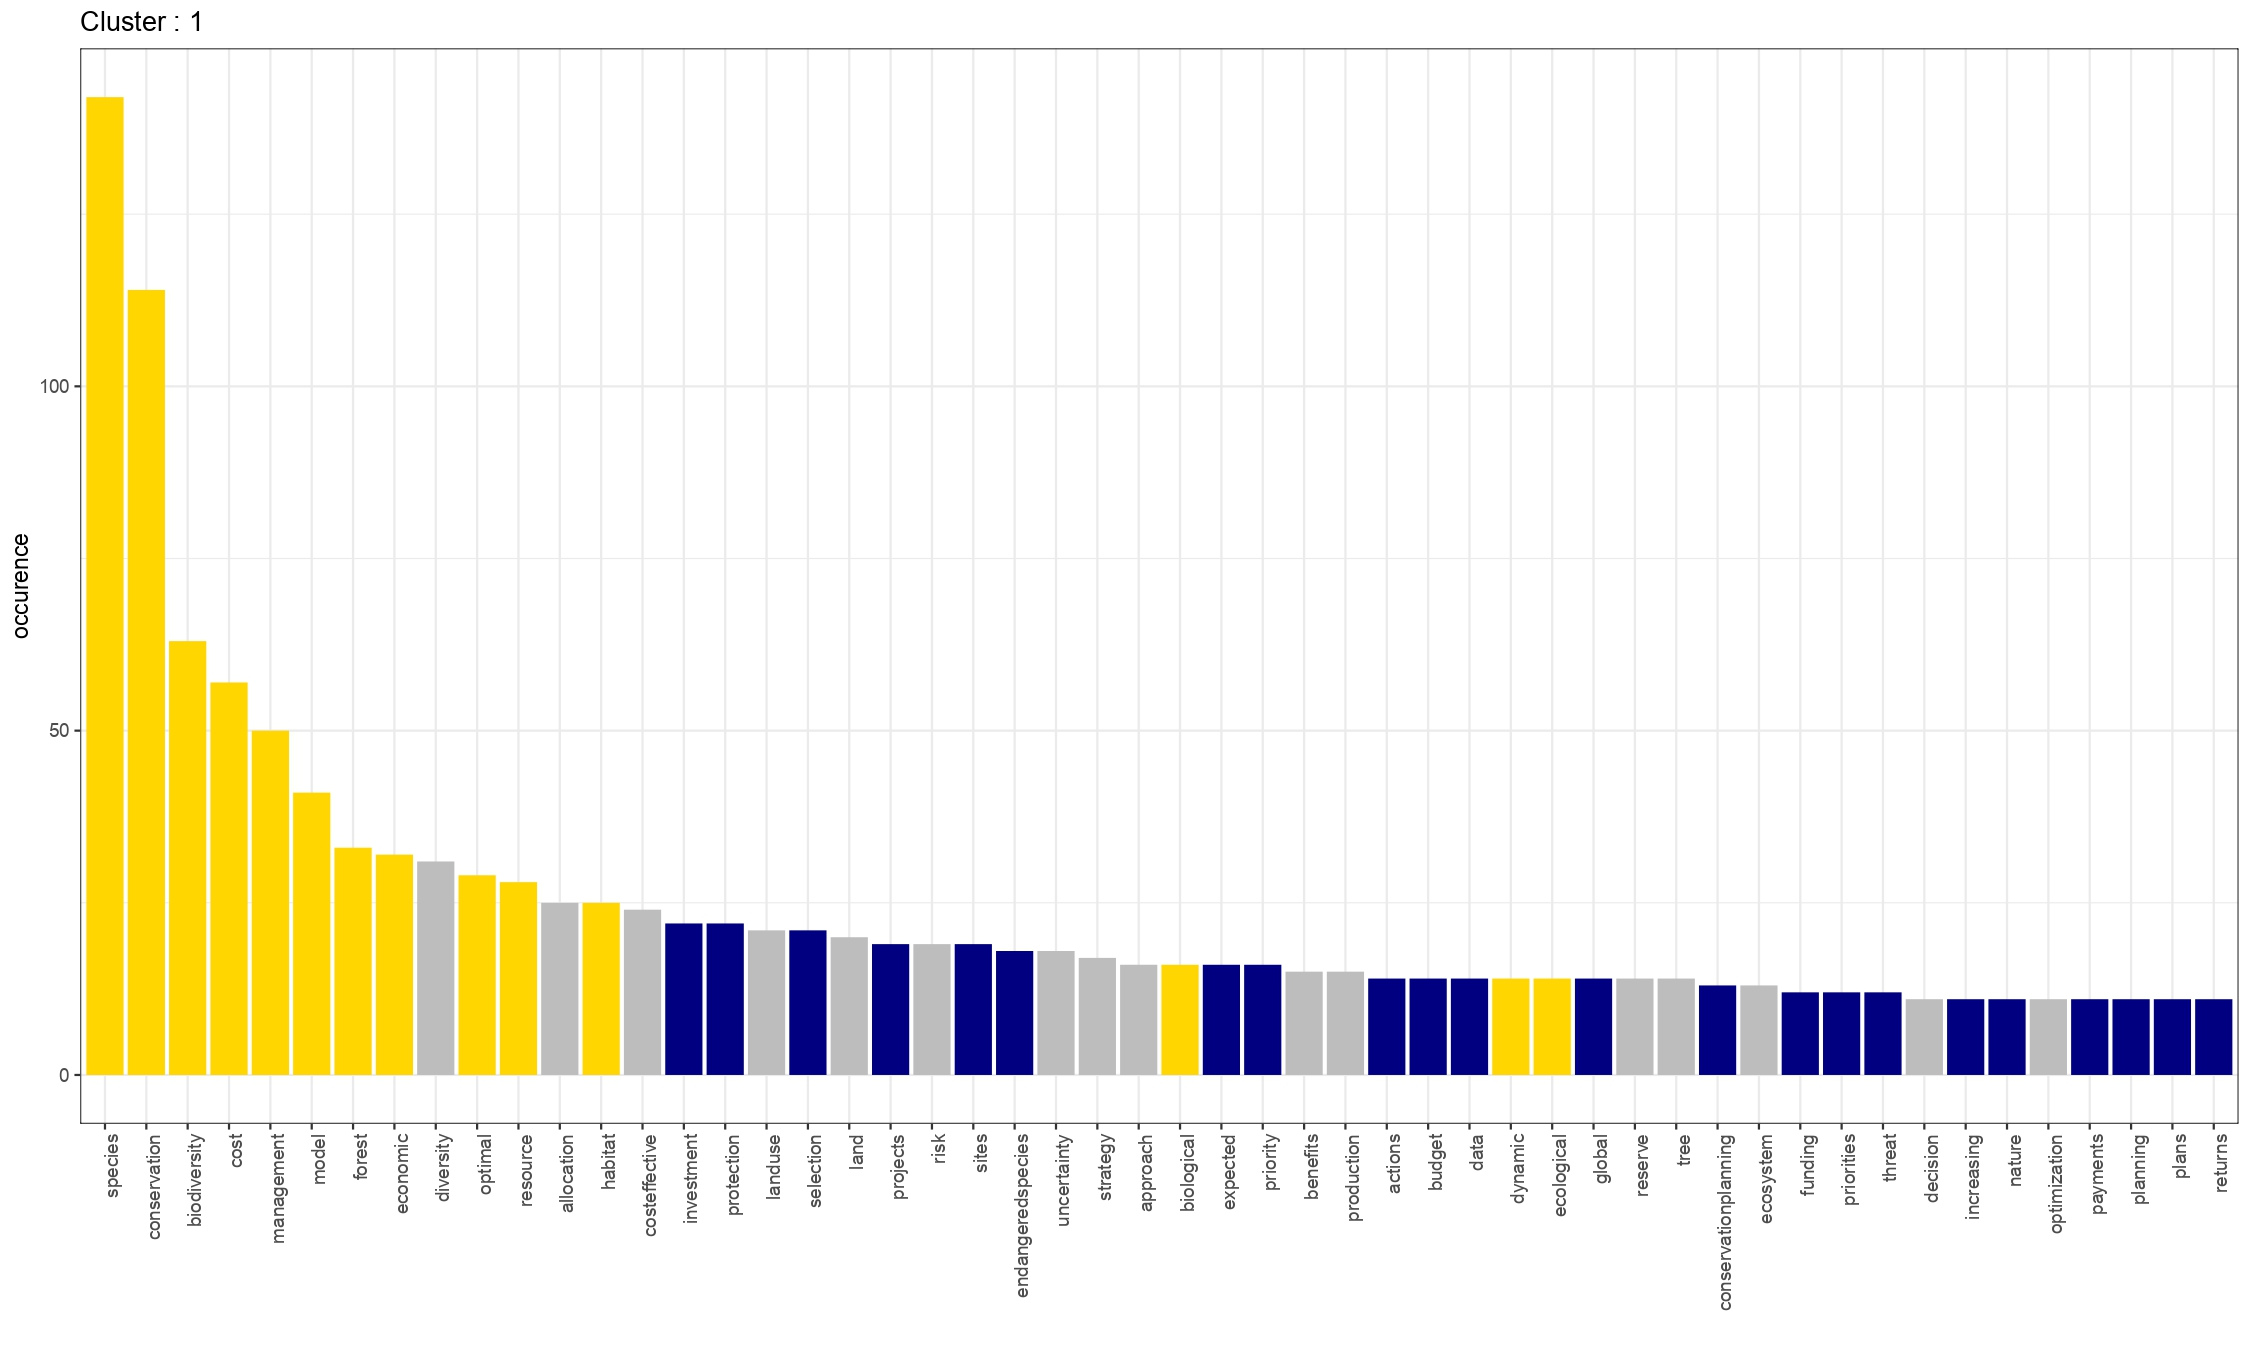
\includegraphics[width = .8\textwidth]{figures/review/occurence_kmodes_new_1_n50_common.png}\\
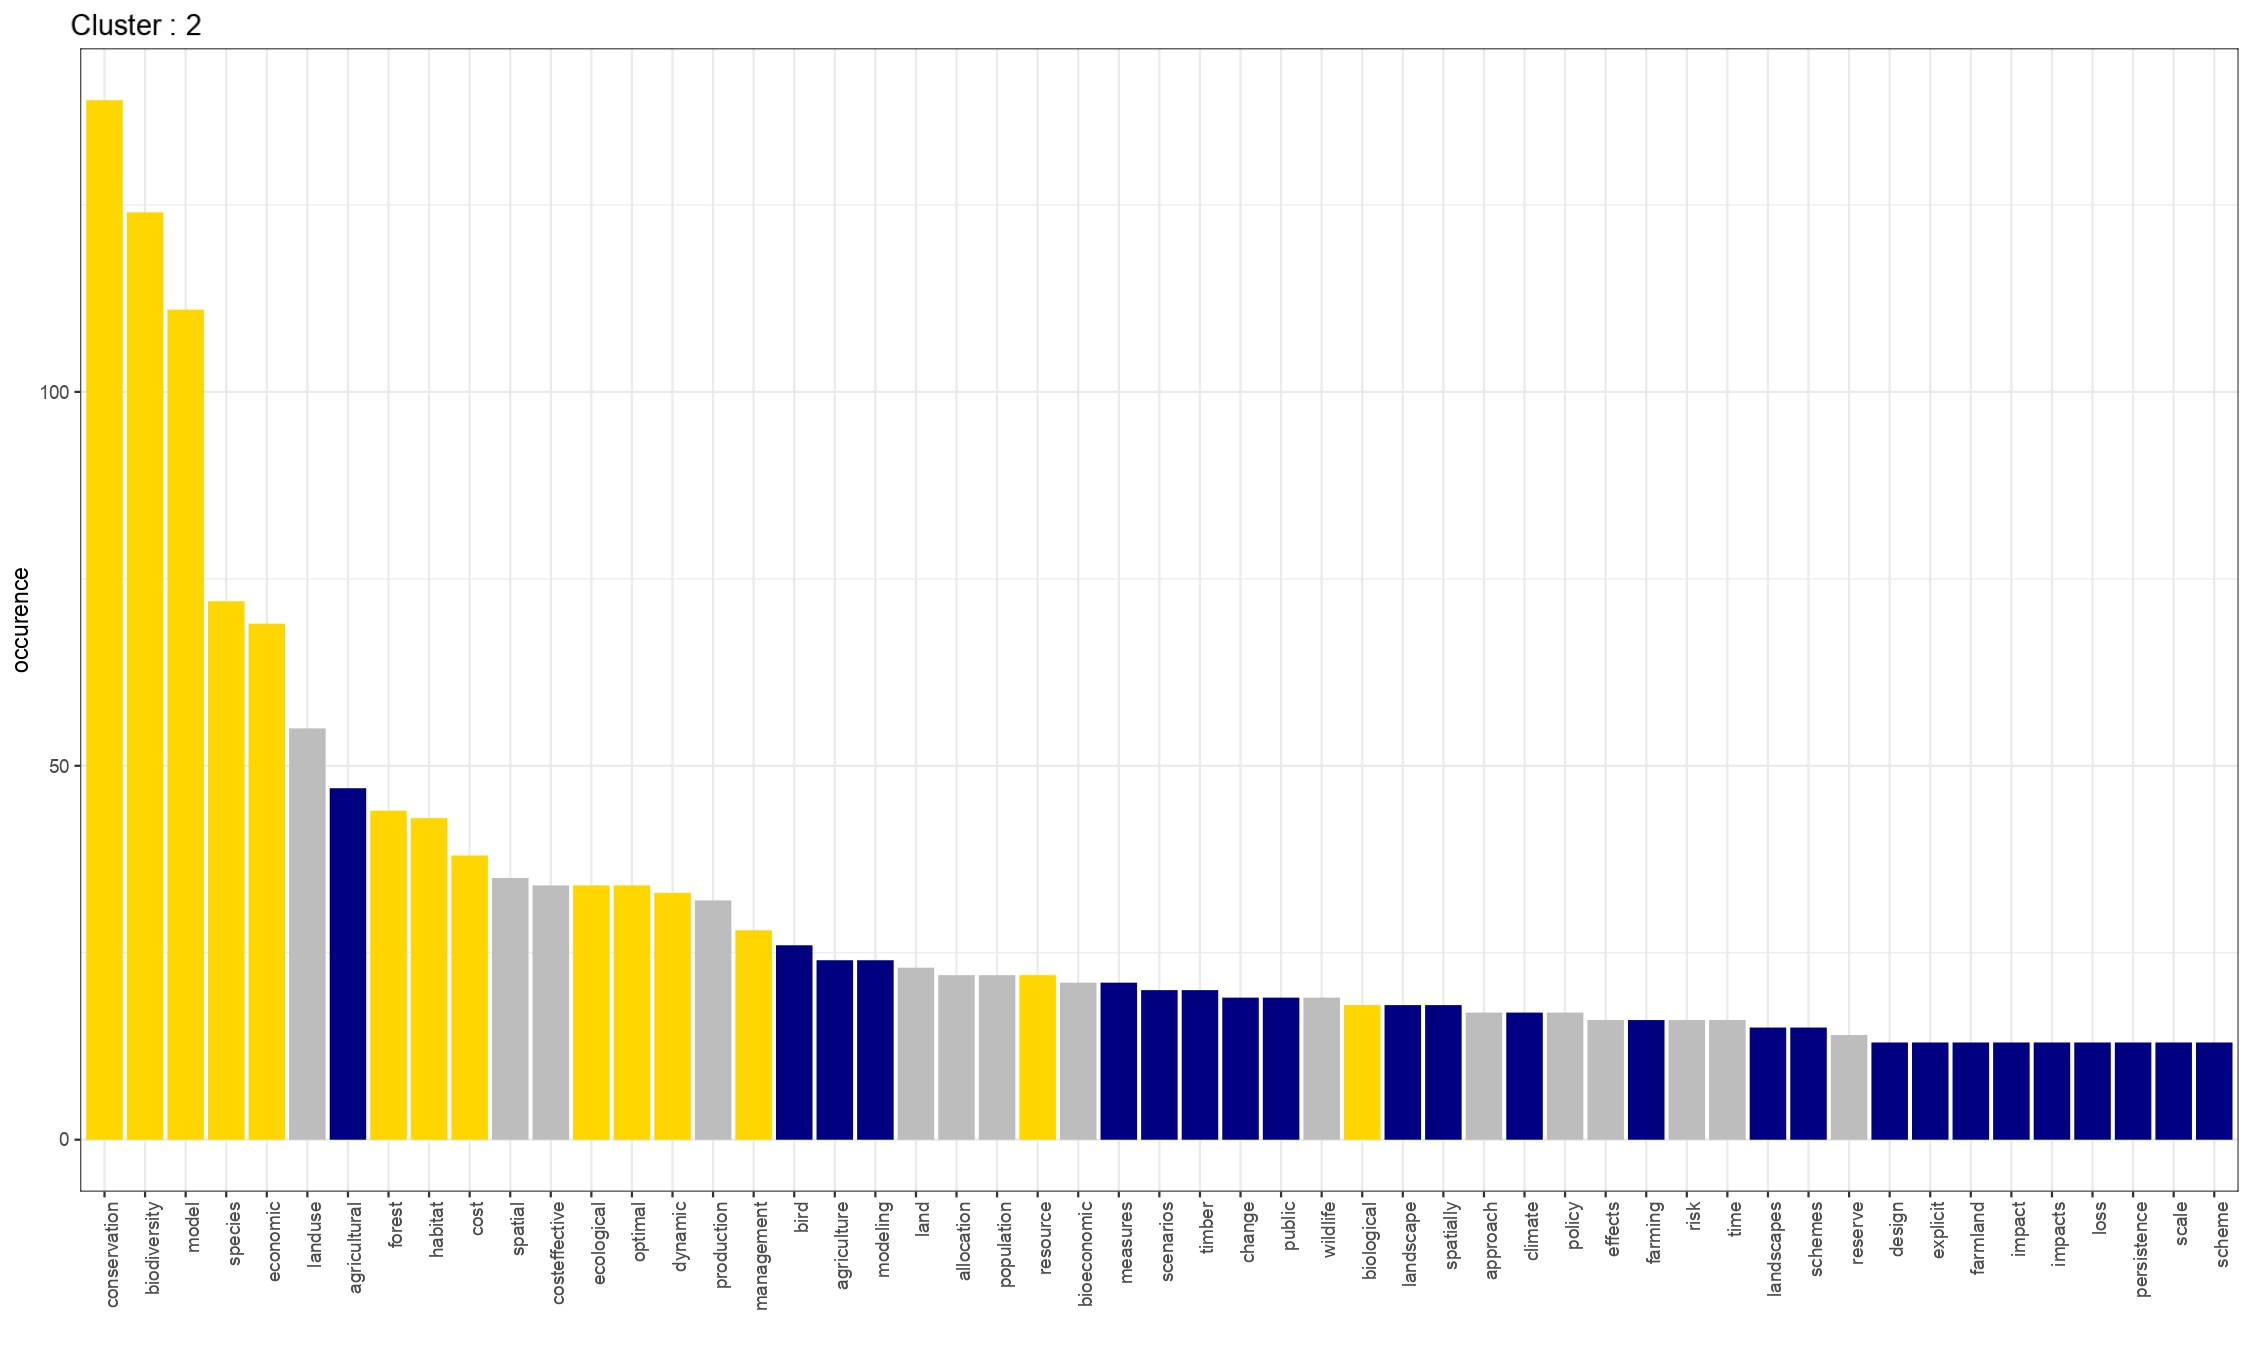
\includegraphics[width = .8\textwidth]{figures/review/occurence_kmodes_new_2_n50_common.png}
\caption{ Distribution profiles of the 50 words the more frequent for methodology-based groups 1 and 2}
\subcaption*{In yellow stand the words in common among the 4 profiles. On the opposite in blue stand the words specific to a profile}
\label{fig:words-profile-1}
\end{figure}

\begin{figure}[h]
\centering
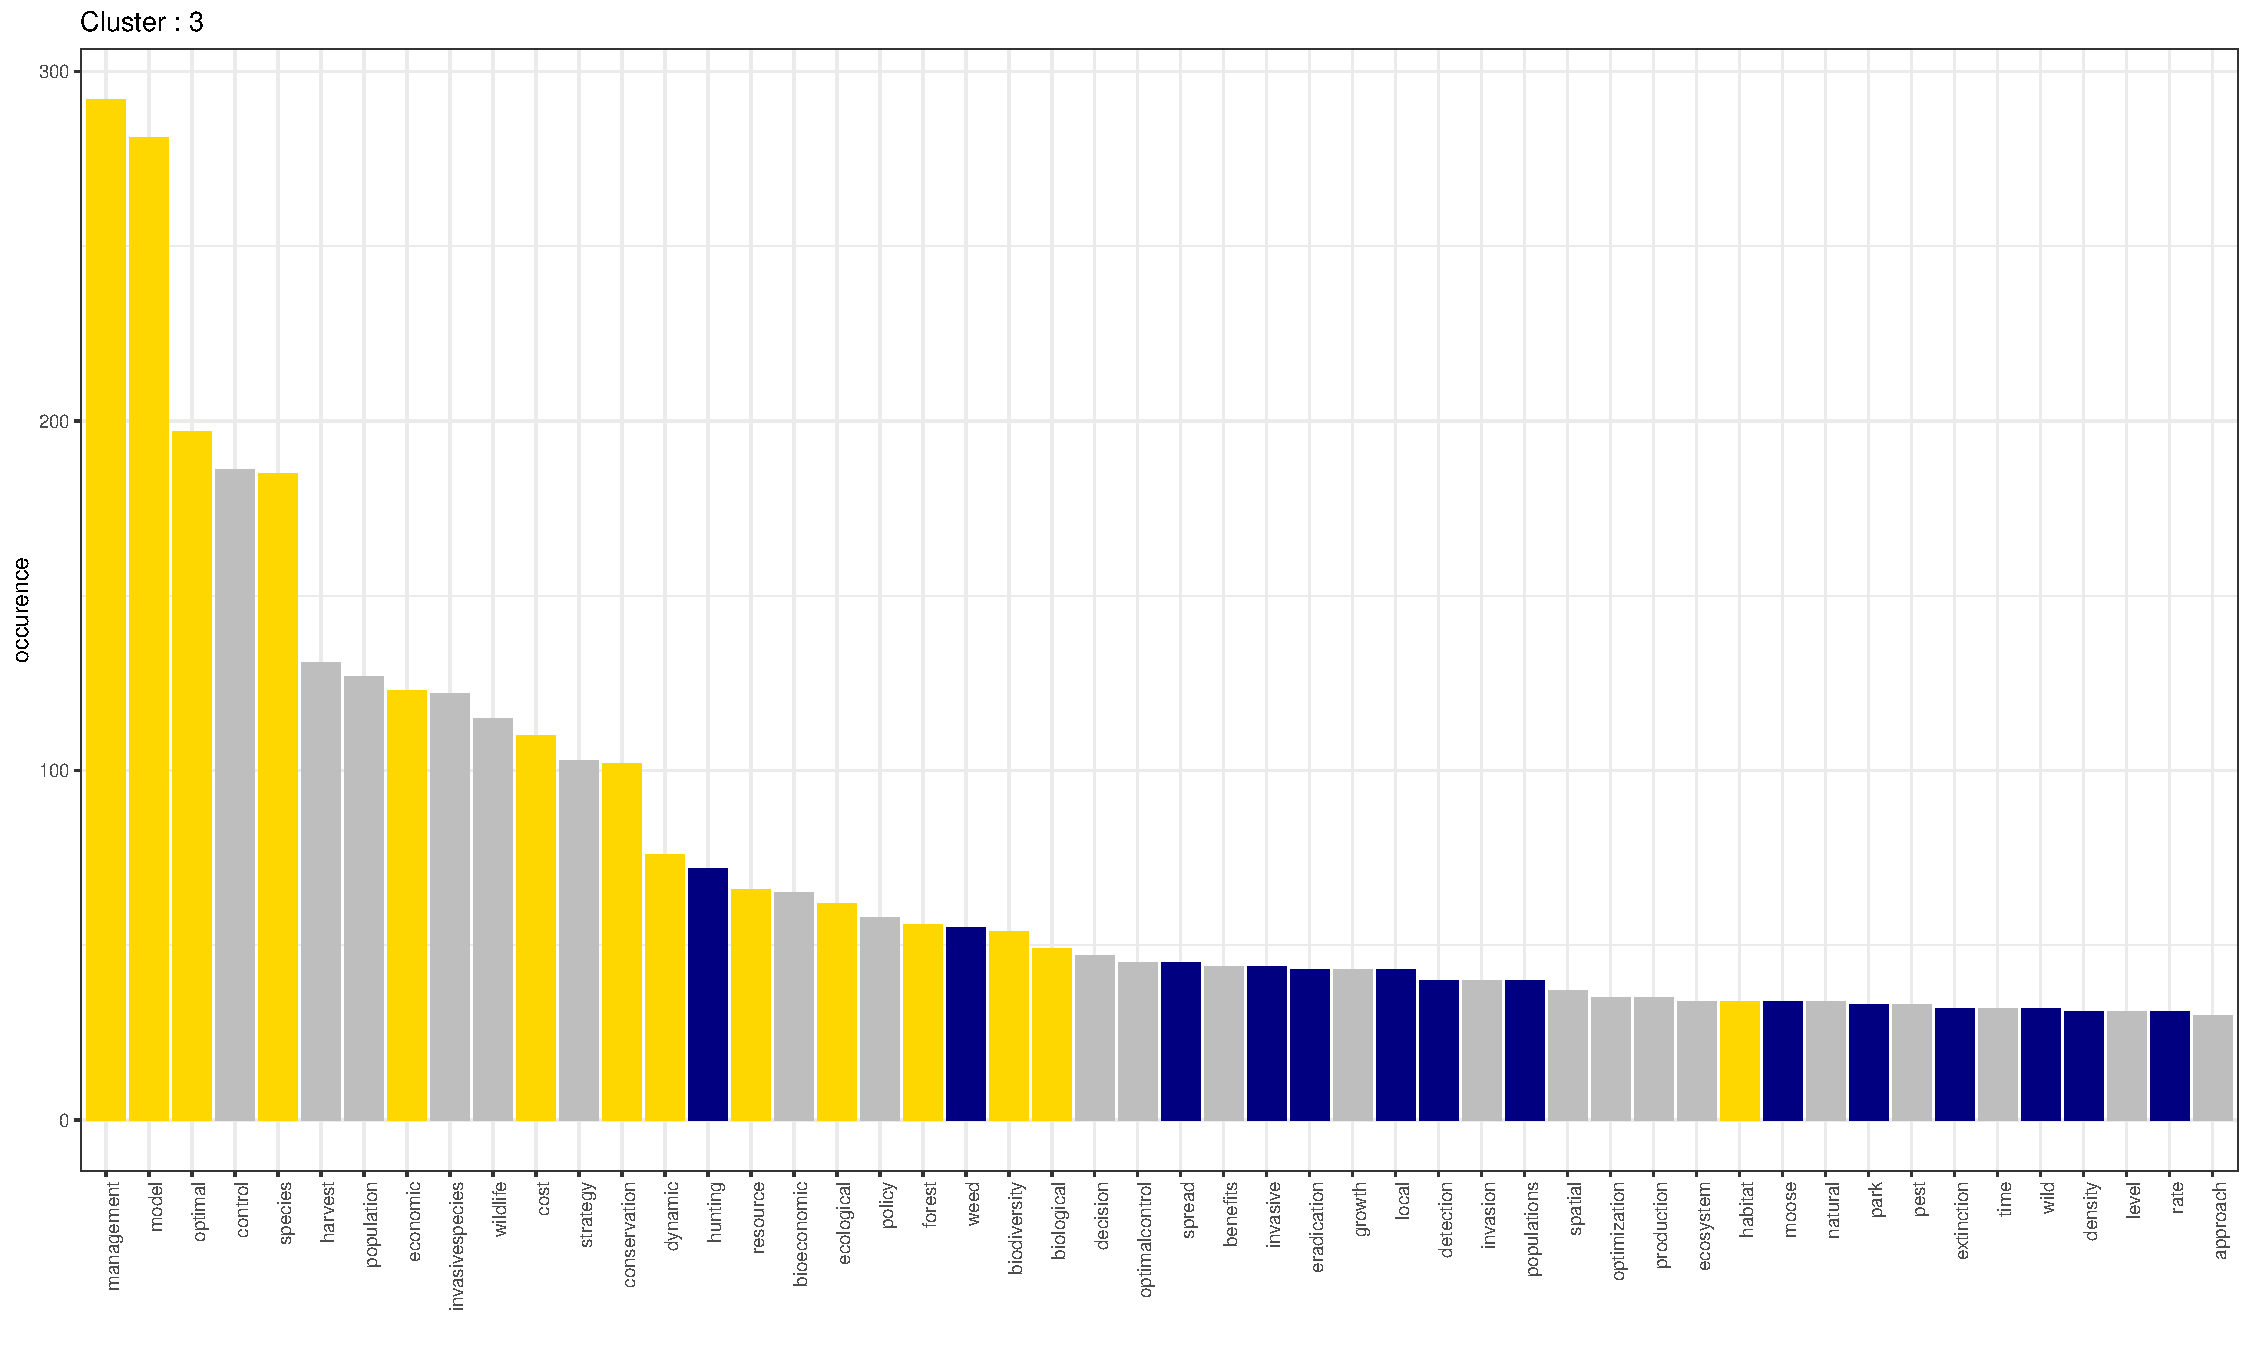
\includegraphics[width = .8\textwidth]{figures/review/occurence_kmodes_3_n50_common.pdf}\\
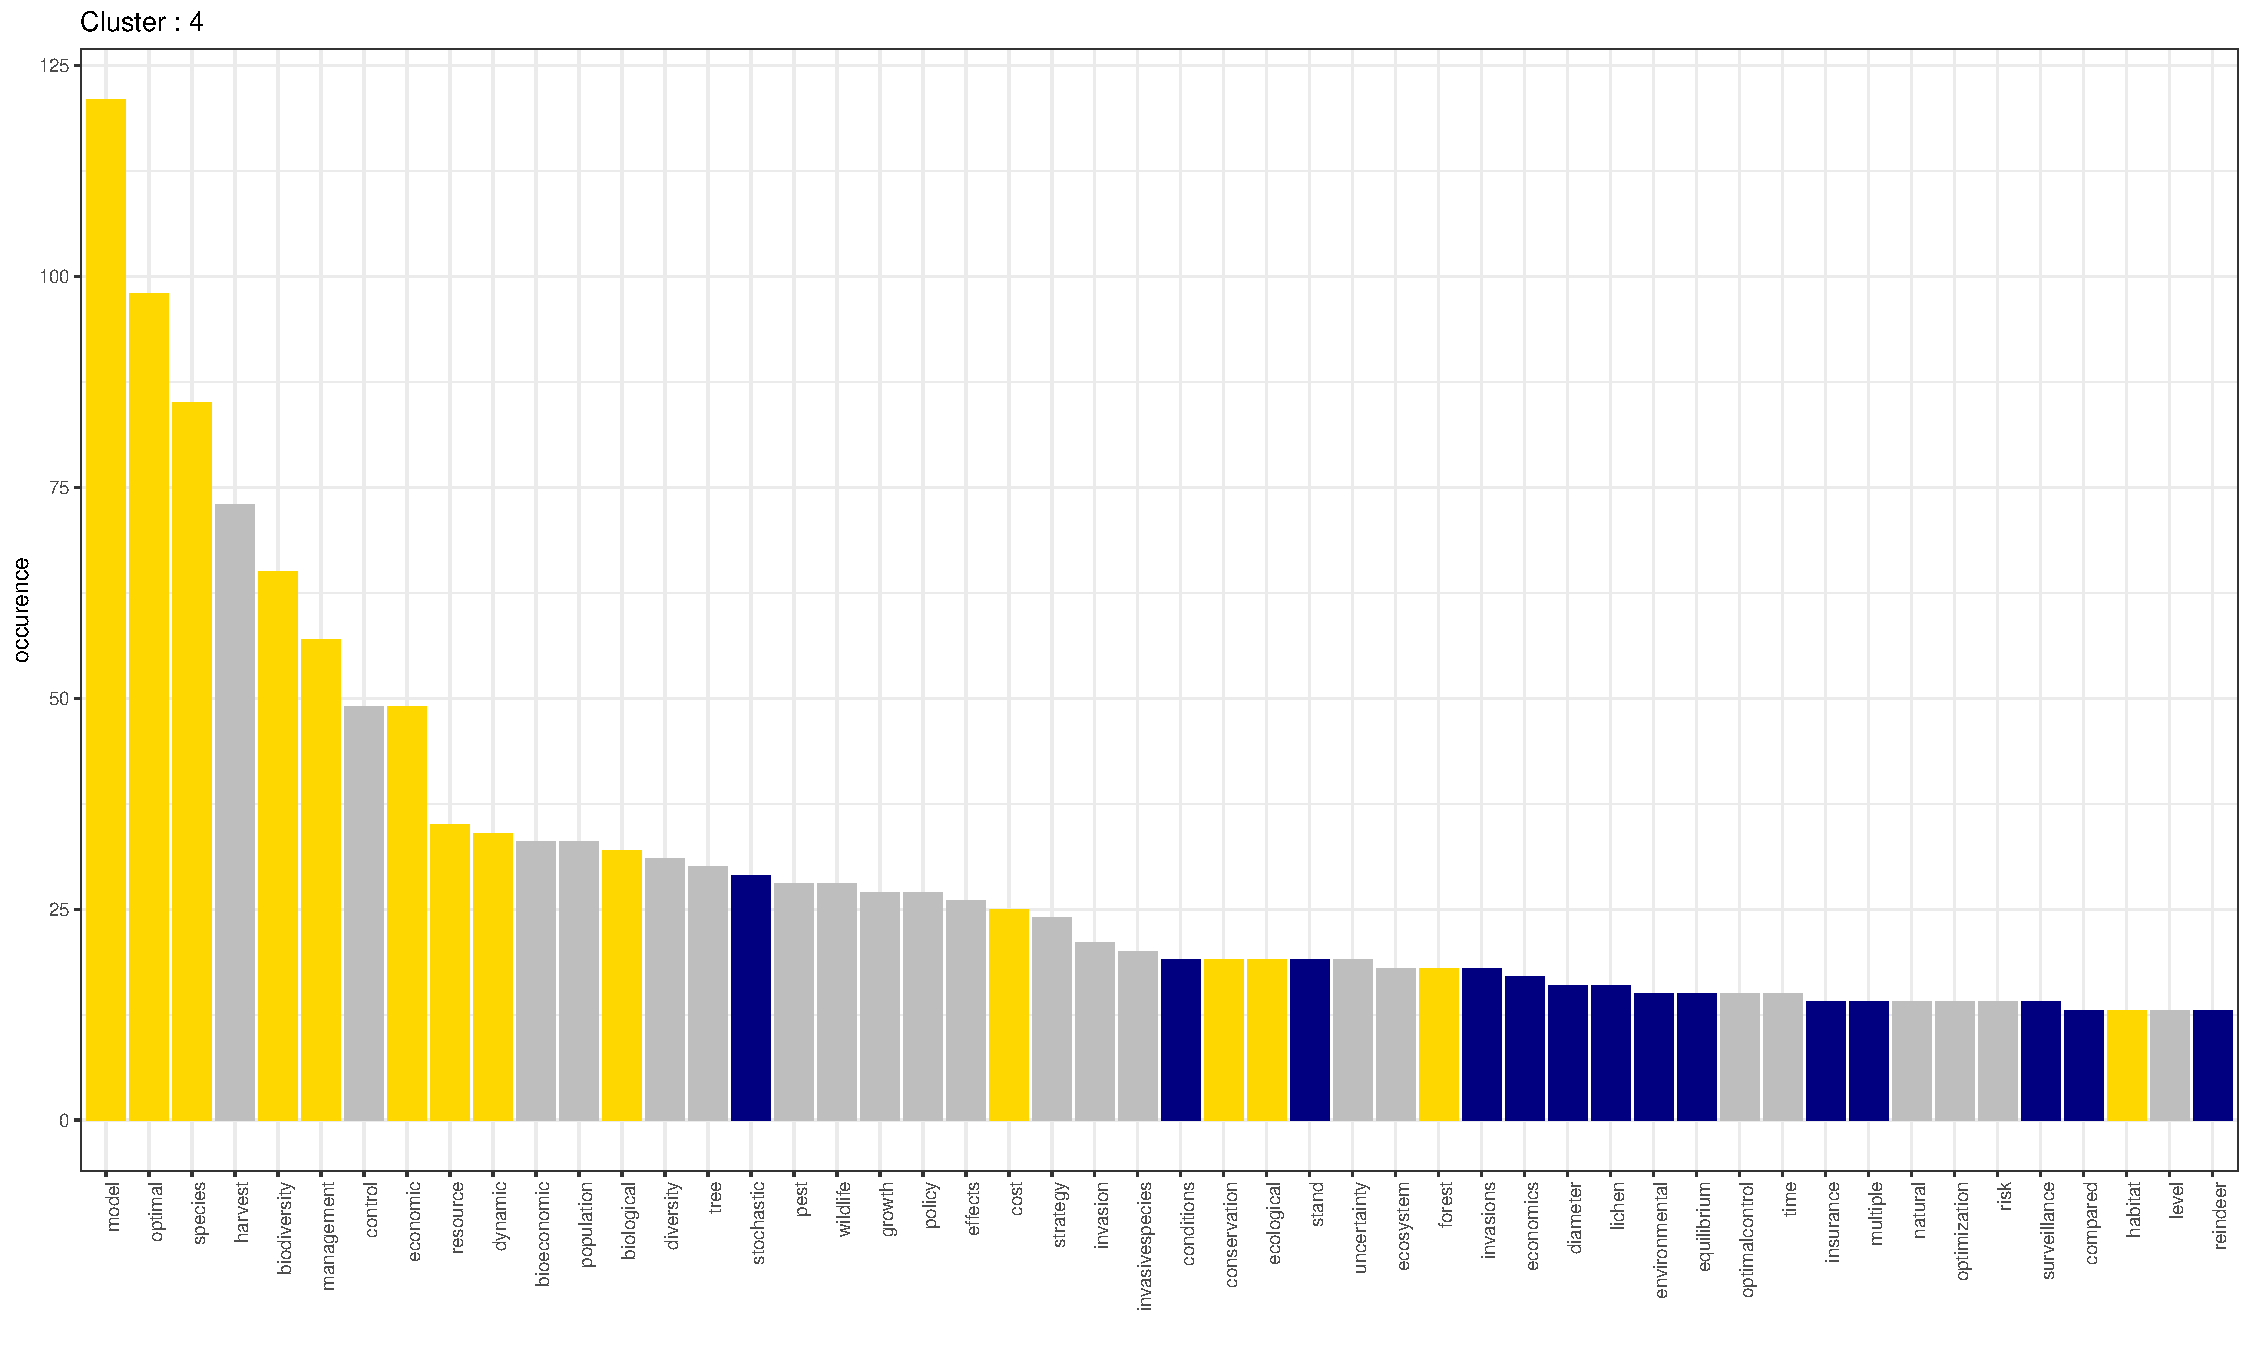
\includegraphics[width = .8\textwidth]{figures/review/occurence_kmodes_4_n50_common.pdf}\\
\caption{Distribution profiles of the 50 words the more frequent for methodology-based groups 3 and 4}
\subcaption*{In yellow stand the words in common among the 4 profiles. On the opposite in blue stand the words specific to a profile}
\label{fig:words-profile-2} 
\end{figure}

\begin{figure}[h]
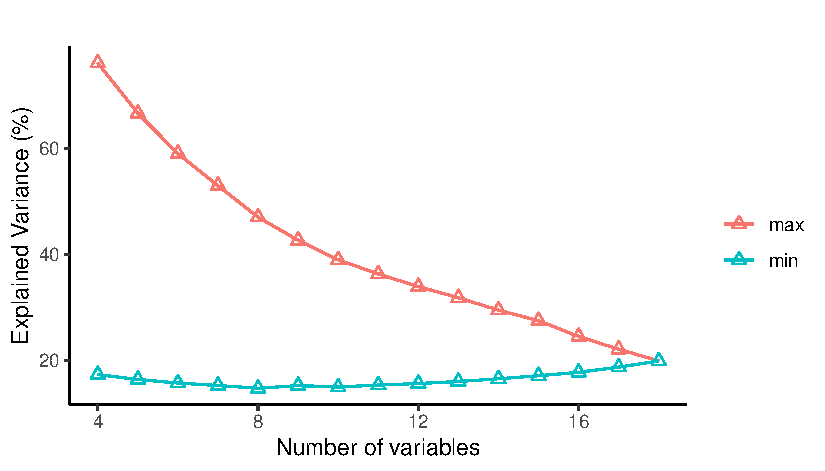
\includegraphics[width=.8\textwidth]{figures/review/variables_variance_enveloppe.pdf}
\caption{\label{fig:nb-crit-methodo} Explained variance function of the number of methodological criteria used in the MCA.}
\end{figure}

\begin{figure}[h]
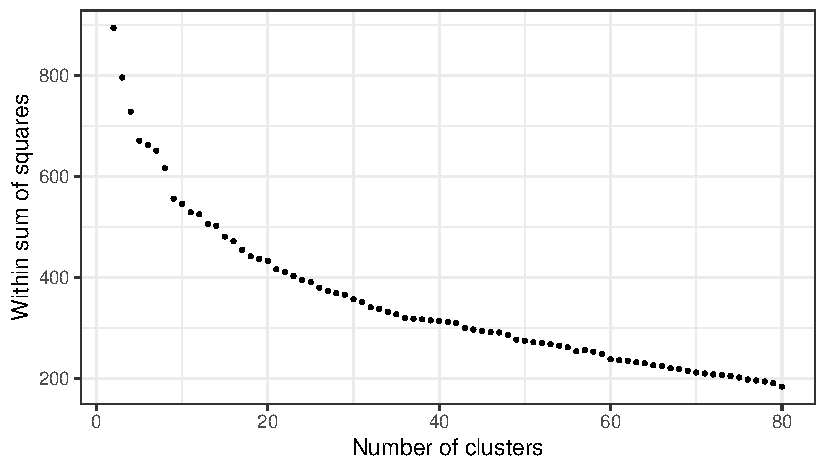
\includegraphics[width=.8\textwidth]{figures/review/kmodes_elbow.pdf}
\caption{\label{fig:cost-function} Cost function of the K-modes.}
\end{figure}

\begin{figure}[h]
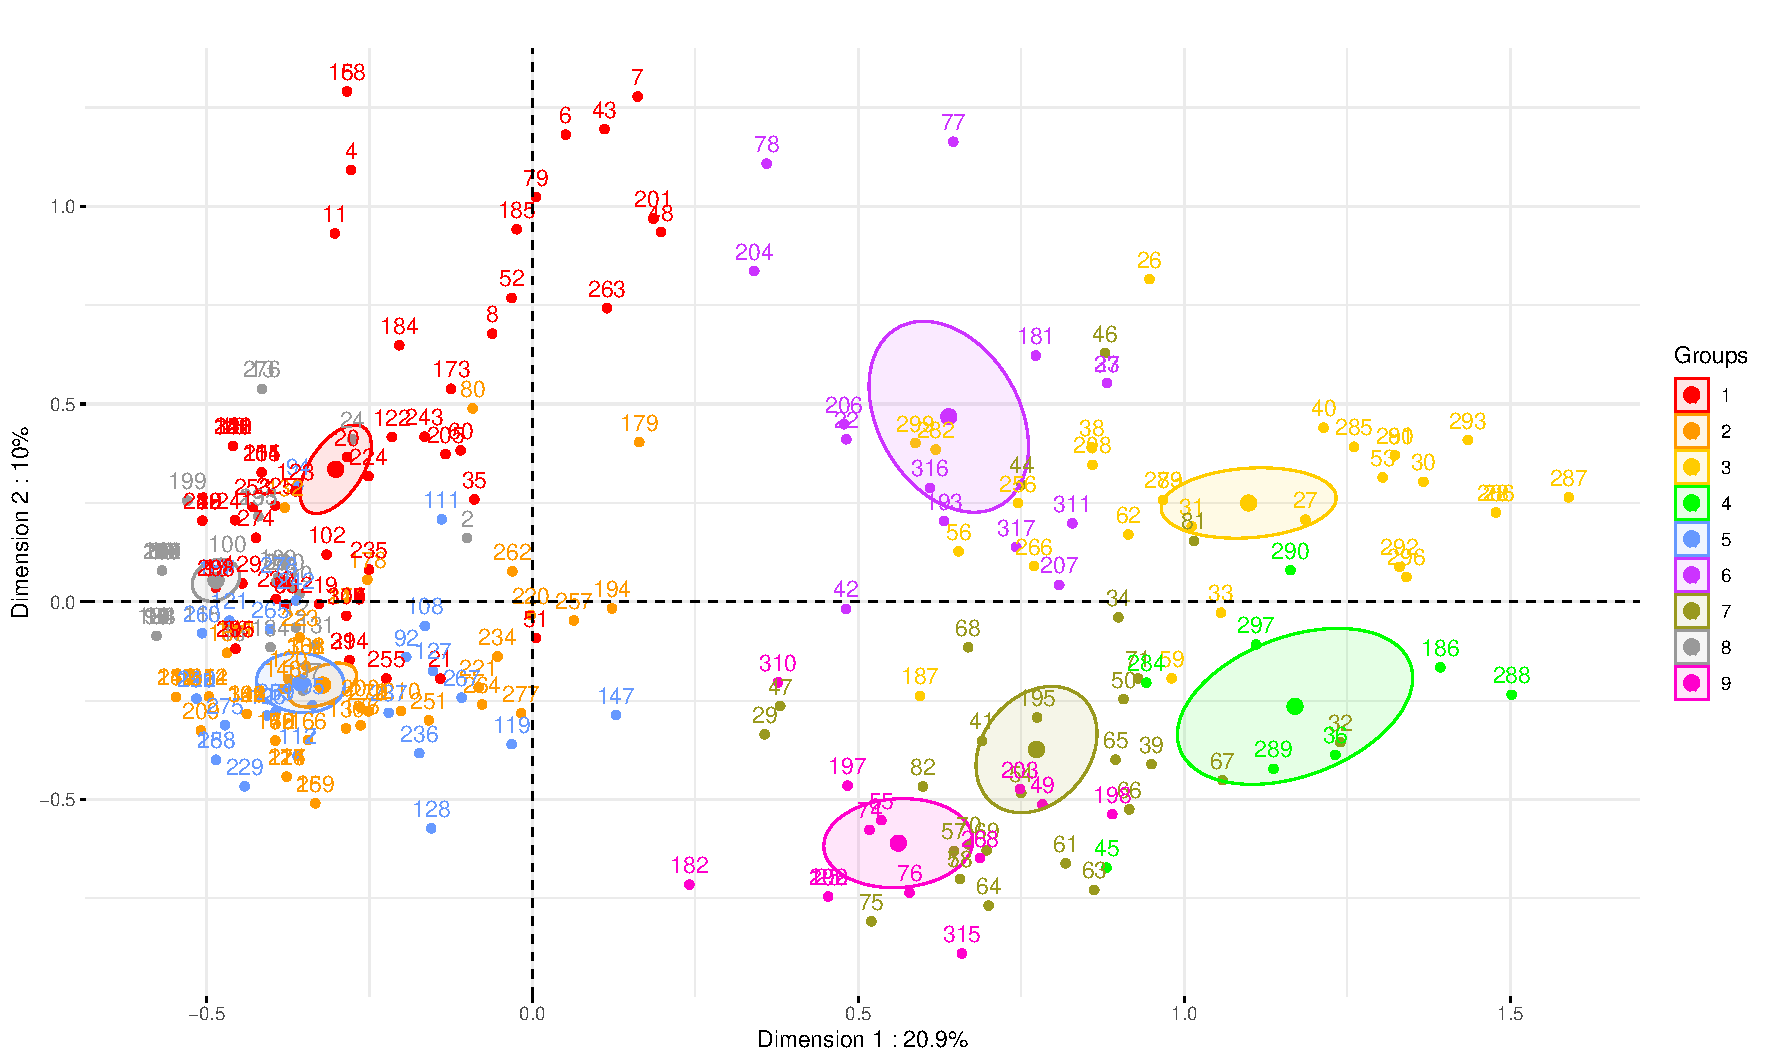
\includegraphics[width=.8\textwidth]{figures/review/mca_ind_automated_kmodes9.pdf}
\caption{\label{fig:MCA-9groups} Multiple Correspondence Analysis (MCA) running on 12 methodological criteria and 9 groups.}
\end{figure}
	\cleardoublepage
	\chapter{Little downside and substantial gains result from farming of \textit{Totoaba Macdonaldi}}

\begin{center}
\begin{minipage}{0.9\textwidth}
\singlespacing
This is article is under review at \textit{NPJ Ocean Sustainability} and is joint work with Julia M. Lawson (co-first author), Andrew Steinkruger, Miguel Castellanos-Rico, Garett M. Goto, Miguel A. Cisneros-Mata, Erendira Aceves Bueno, Matthew M. Warham, Adam M. Sachs and Steven D. Gaines\\\\
\end{minipage}

\textbf{Abstract}\par
    \vspace*{.2cm}
    \noindent
    \begin{minipage}{0.9\textwidth}
    \singlespacing
Illegal wildlife trade poses a growing threat to species globally. Where bans or policy instruments have failed, conservation farming has been considered, which aims to reduce illegal poaching by “flooding the market” with farmed product. However, predicting if farming will succeed necessitates a holistic understanding of how supply and demand interact and how markets will respond. Poaching and illegal trade for totoaba (Totoaba macdonaldi), currently dominated by a Mexican monopolist cartel, has continued unabated despite half a century of prohibitions on international trade and domestic fishing. We investigate if farming can reduce poaching and support a healthy wild population by extending a flexible bioeconomic model of a three-stage illegal supply chain: poachers sell to traders (i.e., middlemen or cartels) who sell to end-markets. While we show under the monopolist a large stable wild population is maintained, this outcome is sensitive to cost parameters. Introducing farming decreases poaching by 29\% or increases poaching by 6\%, and results are robust to changes in cost parameters. Our results upend previous assertions that certain strategic responses will undermine conservation efforts and always result in population collapse. Furthermore, our quantitative framework can be adapted to evaluate conservation farming for other species and market structures.\\\\
Keywords : 
\end{minipage}
\end{center}
    \vfill


\newpage

\section{Introduction}
\onehalfspacing
Illegal wildlife trade is a multi-billion dollar industry that drives biodiversity loss through unsustainable harvest \citep{t_sas-rolfes_illegal_2019}, spreads zoonotic disease \citep{bell_animal_2004}, and threatens animal welfare\citep{baker_rough_2013}. The Convention on International Trade in Endangered Species of Wild Fauna and Flora (CITES) provides a regulatory framework that aims to ensure that international trade of wild animals and plants does not threaten their survival. Yet, for many species, regulatory interventions such as trade bans and controls have failed, and illegal trade in black markets continues to flourish \citep{challender_poaching_2014, challender_towards_2015}. In such instances, supply-side interventions such as conservation farming can theoretically bolster conservation by “flooding the market” with farmed products, leading to reduced market prices and lower poaching incentives \citep{gentry_looking_2019, phelps_framework_2014, tensen_under_2016}. Supply-side interventions have occasionally succeeded at reducing poaching and recovering wild populations – e.g., vicuña and spotted cat \citep{iucn_world_2000, sahley_biological_2007} – but they have also failed – e.g., green python, African elephant \citep{lyons_wildlife_2011, hsiang_does_2016}. Uncertainty around conservation outcomes from market-based approaches has led to continued reliance on trade bans and controls that are often ineffective at reducing poaching.
\\
Determining whether farming will succeed or fail requires a holistic understanding of a specific illegal wildlife market1, including the interplay between market conditions and ecological criteria \citep{challender_understanding_2015}. Studies have pointed to a common set of farming pitfalls. Species with slow individual growth rates and low fecundity are often unable to grow supply quickly enough to displace illegal products. Further, if poaching is very inexpensive, it is impossible for farming to undercut prices 6,8 – e.g., dried seahorses are ‘free’ to poach when retained as bycatch \citep{lawson_low_2017}. Demand-side concerns are focused on substitutability between farmed and wild products. Consumers of wildlife for medicinal or conspicuous purposes often prefer wild products for greater perceived potency or associated social status \citep{dutton_stated_2011, gratwicke_attitudes_2008, fabinyi_historical_2012}. Here, we develop a quantitative framework that comprehensively considers all these pitfalls while accounting for detailed species-specific and market information. 
\\
Another critical factor in driving the success or failure of farming is market structure: illegal markets are often characterized by imperfect competition – where an individual trader or a small number of traders (i.e., middlemen, cartels, gangs, or other criminal organizations) dominate illegal trade and exert significant control over market prices. A bioeconomic model that predicts how imperfectly competitive markets will respond to competition from farming was developed almost two decades ago \citep{bulte_economic_2005, damania_economics_2007}. Predicted strategic responses depend on how a trader chooses to compete with farming. If a trader responds by price setting (an aggressive response where the trader tries to undercut farmed prices and take market shares), then poaching pressure will increase and can lead to the collapse of the wild population. On the other hand, if traders respond by quantity adjustment (a mutually beneficial response where the trader competes on the amount of output produced, letting market prices adjust), poaching pressure is reduced and wild populations have the possibility to increase. This model has been widely used to both justify \citep{biggs_legal_2013,abbott_can_2011} and discourage \citep{tensen_under_2016} prospective farming initiatives. The authors of the original bioeconomic model concluded that farming is a perilous coin toss \citep{bulte_economic_2005, damania_economics_2007}. Here, we expand upon this model and reach a different conclusion: that farming can maintain large, stable wild population sizes that are robust to changes in cost structure under both types of competition. Furthermore, quantity adjustment yields substantial decreases in poaching and is the more likely response because prices and profits are higher than under price setting \citep{singh_price_1984}.
\\
We explore the biological and economic performance of conservation farming for totoaba swim bladder in the context of illegal poaching and trade under different market conditions \citep{froehlich_conservation_2017}. Specifically, we examine the evolution of poaching and wild totoaba biomass, as well as prices and profits for different economic actors. The lifecycle for totoaba has been successfully closed in aquaculture, and the species is currently farmed in Mexico for domestic meat production. Totoaba is endemic to Mexico’s Gulf of California and is threatened by a lucrative illegal international trade for its large swim bladder \citep{c4ads_hooked_2017, environmental_investigation_agency_citess_2019, environmental_investigation_agency_collateral_2016} . A single totoaba swim bladder can sell for up to \$80,000 USD per kilogram in Chinese end markets, where it is purchased for special occasions, gifting, and speculative investment \citep{elephant_action_league_operation_2018, sadovy_de_mitcheson_emerging_2019, martinez_mexican_2021}. For nearly half a century international trade for totoaba has been prohibited, and the legal totoaba commercial fishery has been closed. However, illegal fishing and trade continue and are controlled primarily by a single criminal organization (a cartel) that will likely respond strategically to farming \citep{damania_economics_2007,felbab_brown_organized_2022}  

\begin{figure}[H]
    \centering
    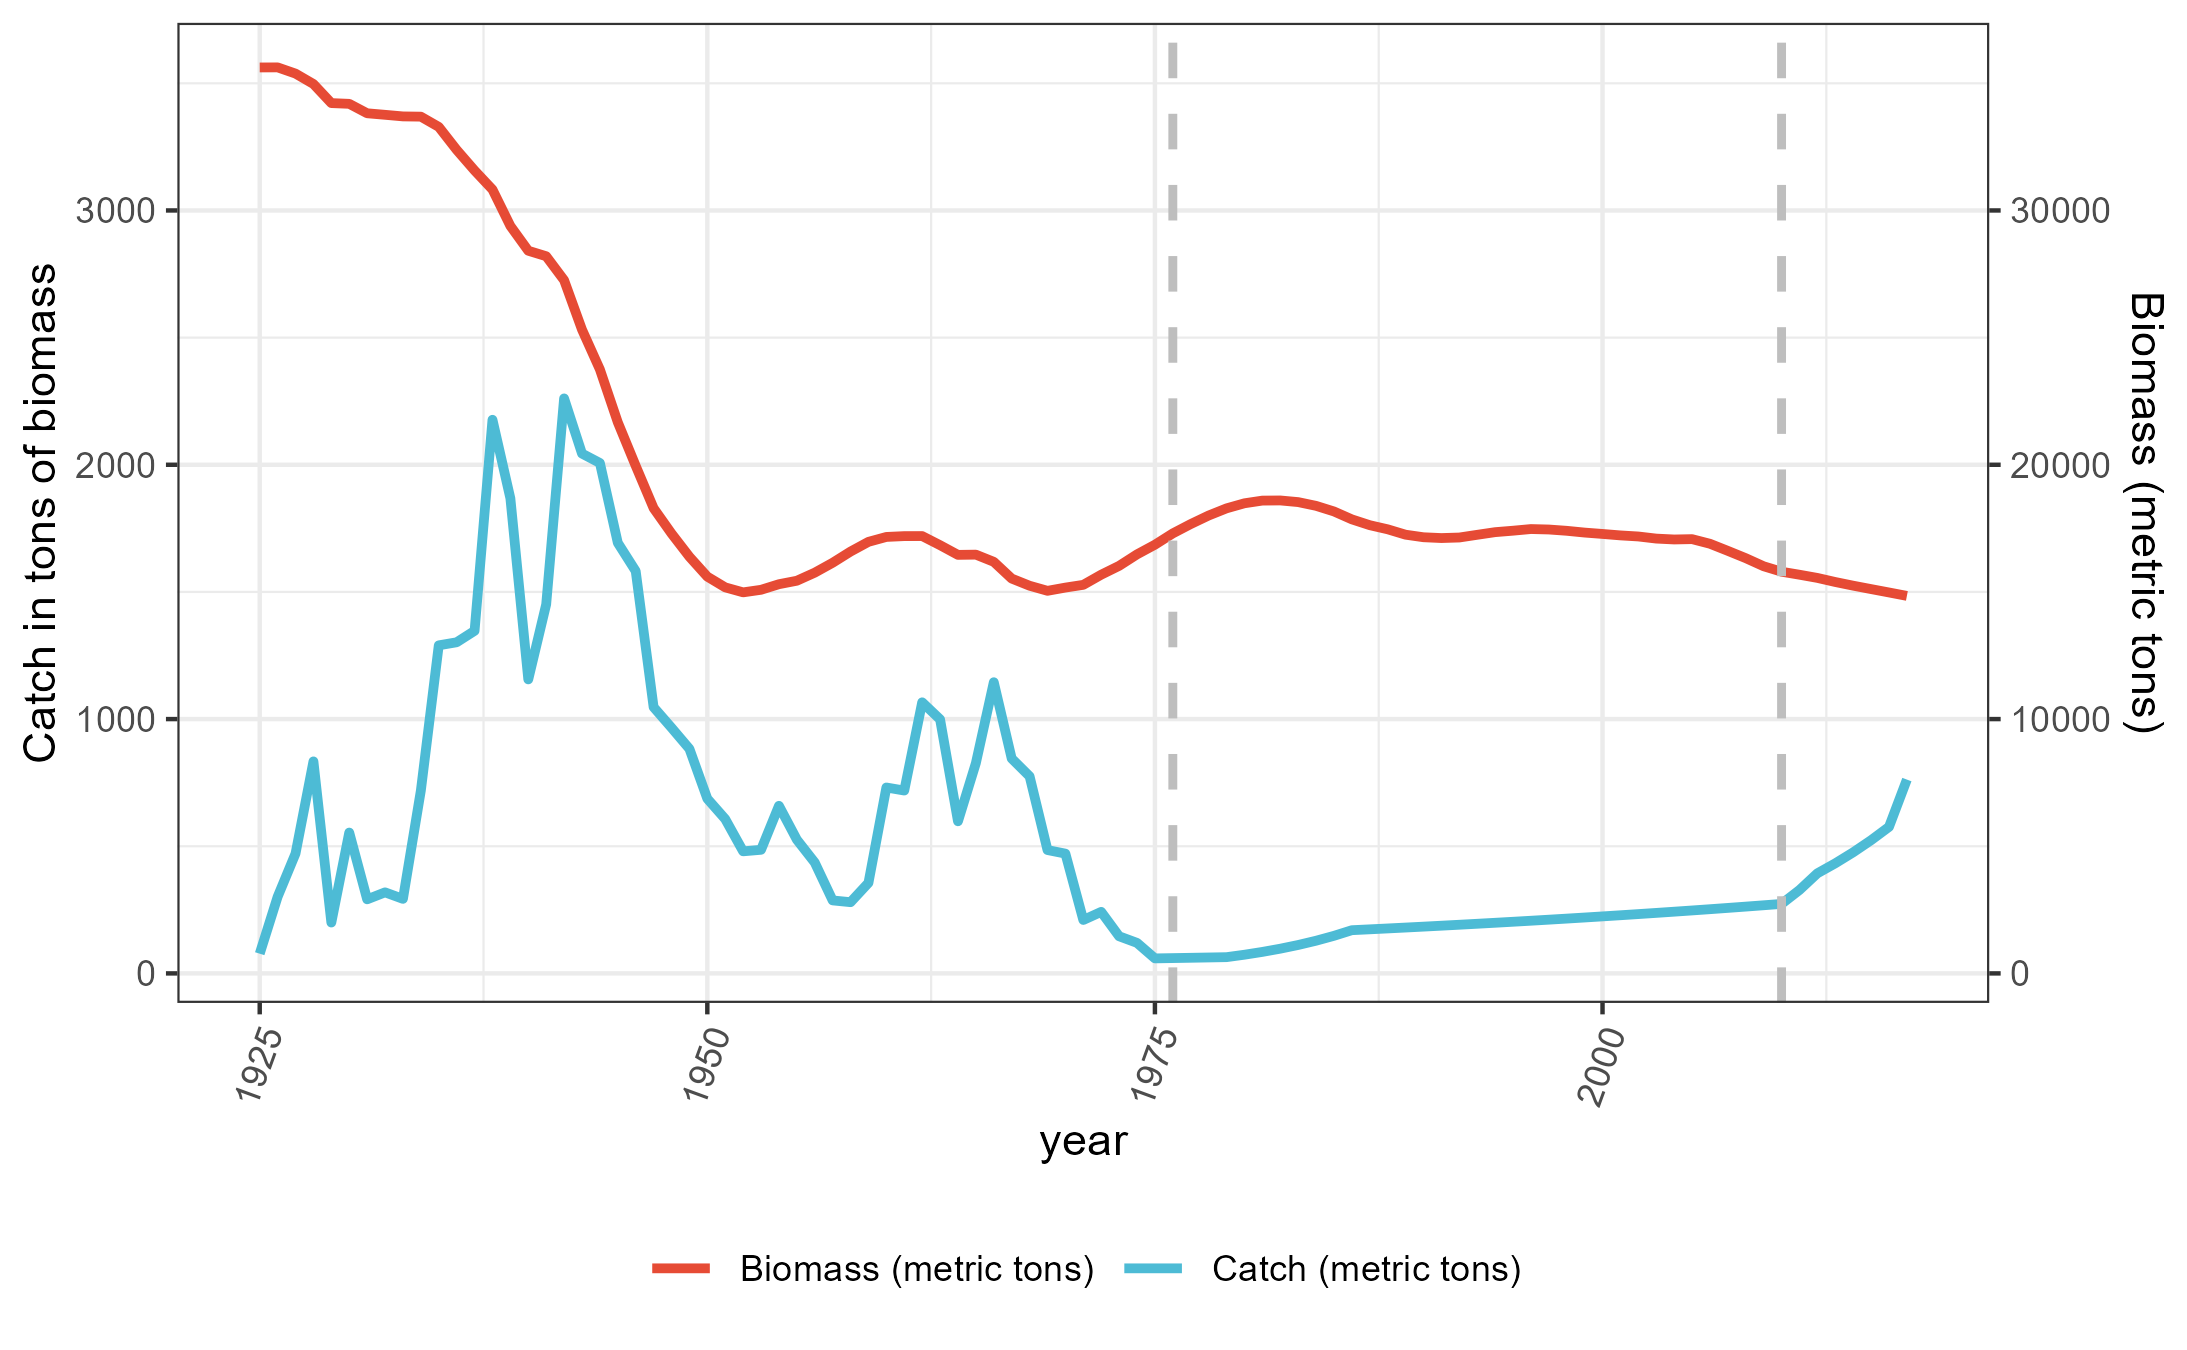
\includegraphics[width=0.8\linewidth]{figures/totoaba/Trends_stock_catch.png}
    \caption{Evolution of totoaba population and catch over time}
    \subcaption*{Dashed lines represent listing as CITES Appendix II species, and cartel takeover, respectively}
    \label{fig:trends_catch}
\end{figure}

There is an urgent need to reduce poaching for totoaba, as the vaquita (Phocoena sinus), a porpoise also endemic to the upper Gulf of California, is caught as bycatch in gillnets used to catch totoaba. The vaquita is on the brink of extinction as there are now fewer than fifteen individuals remaining \citep{rojas-bracho_more_2022}. Furthermore, illegal trade has had negative social welfare consequences, as cartels are increasingly extorting Mexican fishing communities \citep{felbab_brown_organized_2022}. Despite Mexico’s attempts to stop totoaba poaching through various enforcement mechanisms, the country recently received wildlife trade sanctions for taking inadequate action \citep{rojas-bracho_vaquitas_2013,cites_notification_2023}. Conservation farming presents a legal alternative to reduce illegal fishing by manipulating market structure. 
\\
We assemble and leverage a unique wealth of information on the totoaba stock, poaching sector, and farming sector to estimate the effects of market structure on poaching harvest and stock biomass. We focus on the market structure that best characterizes the totoaba trade – a vertical monopoly where a single monopolist trader controls the entire supply chain – and evaluate how this trader will respond strategically to competition from farming. We also show how to identify an effective policy space, where all supply, demand, and market structure parameters align to ensure that conservation farming will reduce poaching. Our results challenge long-standing model conclusions \citep{bulte_economic_2005, damania_economics_2007}, thereby disrupting widely-held beliefs about the impacts of conservation farming. In particular, previous studies cautioned that when a trader responds to farming through price setting, the wild population always declines dramatically. In contrast, we find that for totoaba, price setting can maintain a stable and large population given that as the population size decreases, fishing costs increase. To ensure low retail prices, traders must limit the price they pay to poachers and maintain a viable wild population.

\section{Methods}

We examine the effect of market structure and competition on poaching a population of wild animals using the logistic growth function (Figure \ref{fig:figure2}). The poaching harvest function intersects with population growth producing stable and unstable equilibria. If poaching pressure is high relative to population growth (i.e, when demand is large, or poaching costs are low), a single stable equilibrium point is observed with a low wild abundance (an overharvested population). In the opposite scenario, where poaching pressure is low relative to population growth (i.e, when demand is small, or poaching costs are prohibitive), a single stable equilibrium point is observed with a high wild abundance (a healthy population). Between these extremes, two or three potential equilibria can emerge, with uncertain results that depend on the initial size of the population: a large initial population will result in a high abundance equilibrium point, and a small initial population will result in a low abundance equilibrium point.

\begin{figure}[h]
    \centering
    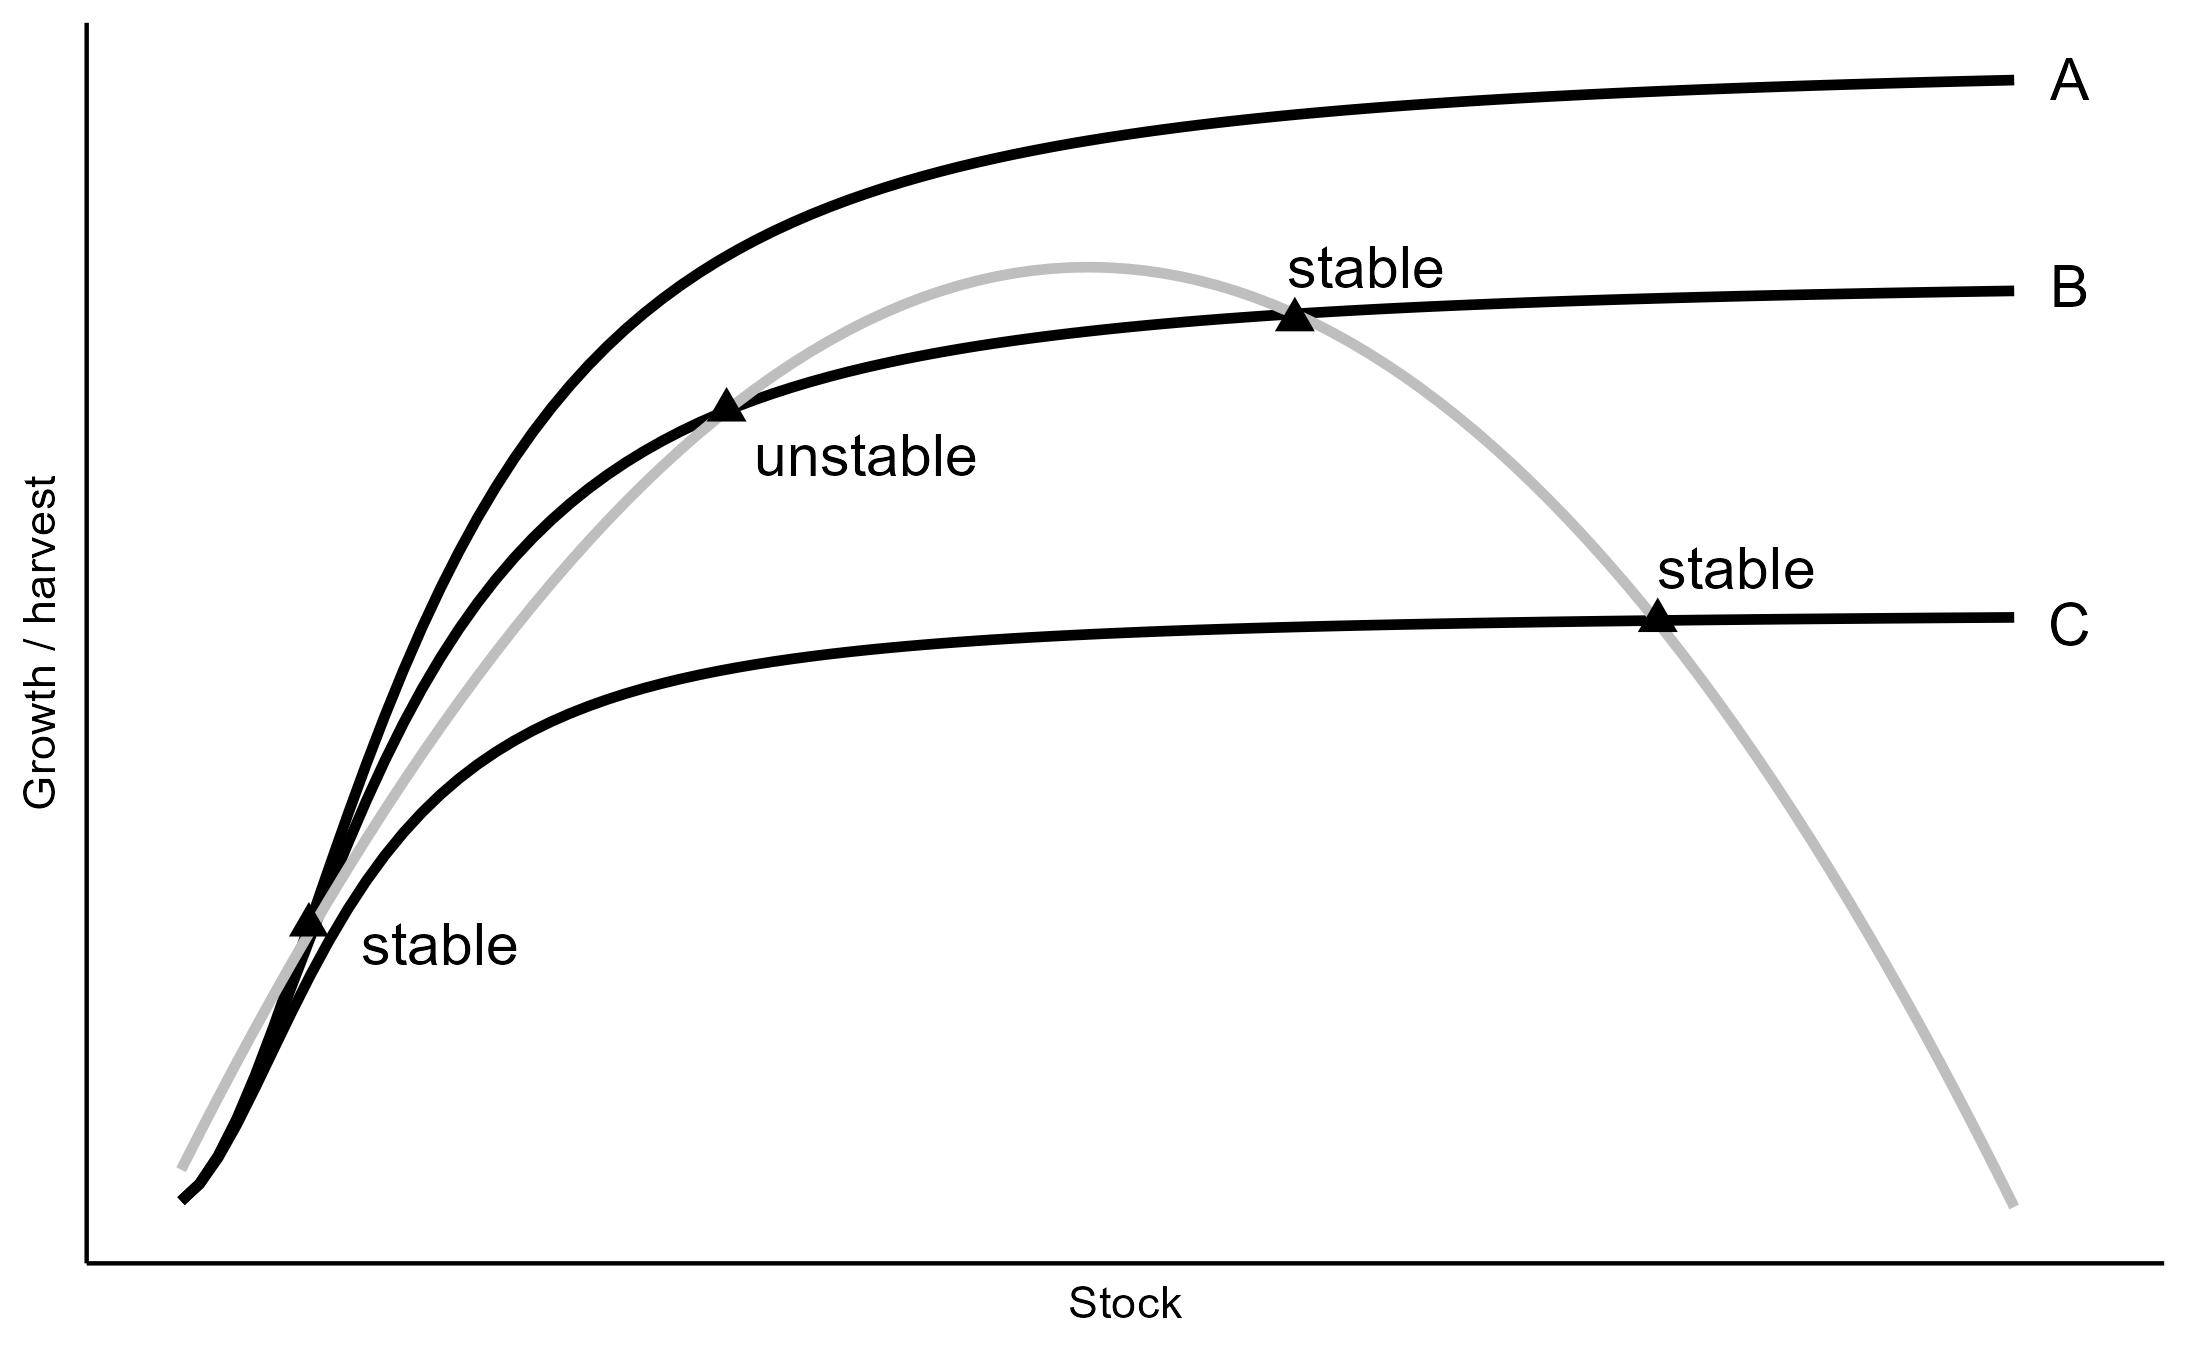
\includegraphics[width=0.85\linewidth]{figures/totoaba/Figure1_potential_equilibria.jpg}
    \caption{Schematic of equilibrium points under different poaching harvest functions}
    \subcaption*{Logistic growth function (light gray) showing equilibria points resulting from three hypothetical poaching harvest functions (black). (A) a single low stable equilibrium point; (B) uncertain outcome, three interior equilibria two of which are stable and one unstable and separating. The long run equilibrium point will depend on the initial size of the population. A large initial population will result in a high abundance equilibrium point, and a small initial population will result in a low abundance equilibrium point; (C) a single high stable equilibrium point.}
    \label{fig:figure2}
\end{figure}

To assess expectations for totoaba, we first calculate equilibrium points for the stock in the absence of conservation farming under vertical monopolistic conditions (hereafter referred to as monopolistic conditions for ease) (Figure \ref{fig:figure3}). A single trader exists in a single location where he is the sole buyer, typical of endemic species such as totoaba \citep{wyatt_differentiating_2020, martinez-alvarado_trafficking_2018}. The trader sells poached harvest on an end market where prices and quantities can be manipulated. 
\\
Next, we add conservation farming to the monopolistic market structure, creating a duopolistic market (Figure \ref{fig:figure3}). We calculate equilibrium points for the totoaba stock if a monopolistic trader responds to conservation farming either in a way that is (a) mutually beneficial by quantity adjustment or (b) aggressive by price setting. From a policy assessment perspective, any scenario where poached harvest produces a single high stable equilibrium point, and the monopolist cartel loses income, presents clear conservation and social welfare benefits.

\begin{figure}[h]
    \centering
    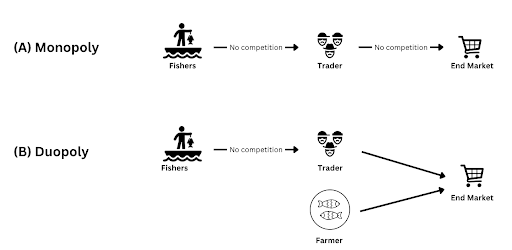
\includegraphics[width=0.85\linewidth]{figures/totoaba/schematic_market.png}
    \caption{Schematic of monopoly and duopoly market structures}
    \subcaption*{(A) monopolistic conditions, where fishers sell to a single trader where they are the sole buyer. This single trader sells poached harvest on an end market where they can manipulate prices and quantities. (B) Next, we add duopoly with farming: A monopolistic trader responds to conservation farming either in a way that is mutually beneficial by quantity adjustment or aggressive by price setting.}
    \label{fig:figure3}
\end{figure}

Here we briefly discuss our methods with an emphasis on the empirical application. Information on our theoretical conclusions from the bioeconomic model we revisited, lemmas and proofs can be found in the Appendix, section \ref{subsection:appendix_toto}. Table \ref{tab:totoaba_functions} summarizes all the functions of the model.  

\subsection{The Poaching Model}

The growth of the fish stock follows a logistic curve and the stock is poached following a Gordon-Schaefer production model. Totoaba population growth parameters were obtained from the 2017 stock assessment, where the carrying capacity ($K$) was $20,226$ mt, and the stock biomass in 2017 was $14,844$ mt \citep{cisneros-mata_evaluacion_2020}. The intrinsic rate of population increase ($r$) was predicted using the \textit{FishLife} package in \textsf{R}, which estimates growth parameters using totoaba-specific life history data from \textit{FishBase} \citep{thorson_predicting_2017}. The growth equation is :
\begin{equation}
g(x) = rx\left(1-\frac{x}{K}\right)
\end{equation}
using a predicted $r$ of $0.20$. We do not consider potential effects of hyperstability of the stock resulting from poaching on seasonal spawning aggregations \citep{erisman_illusion_2011} or age structure.

Poachers optimally determine their effort to maximize their profit, with constant catchability ,$\sigma$, and stock biomass, $x$, obtained from the 2017 stock assessment46, and a linear quadratic cost of effort function, E. The poaching equation is $q =\sigma xE$ where $\sigma =  0.00002. $

Poachers are faced with a linear quadratic cost function $C(E) = W_1 E + W_2E^2$. We calculated two poaching cost parameters $W_1$ (the linear coefficient of the cost function) and $W_2$ (the quadratic coefficient of the cost function) by (a) estimating total and average annual operating costs of the fishing fleet using semi-structured interviews conducted by the authors of this study; and (b) calibrating a linear quadratic cost function that matches historical data and predicts future cost evolution. 

We conducted semi-structured interviews in the upper Gulf of California with two fishing cooperative leaders and four fishers in July and August 2018. These interviews informed annual poaching costs: food and fuel, labor, gear replacement, and bribes paid to fisheries officials. The fishery operates over six months with a variable number of active vessels, monthly fishing days, and sets per day \citep{cisneros-mata_evaluacion_2020}. Poaching costs also include annual fleet-wide costs related to gear confiscations, vessel replacement, and fines, adapted and extrapolated from a summary of law enforcement actions provided by Mexico \citep{noauthor_species_2018}. The cost per fishing trip was estimated to be $\$5,051.26$ during the low season (January and June), $\$8,385.34$ during the mid-season (February and May), and $\$14,386.7$ during the high season (March and April) (supplementary table \ref{tab:costW}). In our analysis we reconstructed a linear quadratic cost function with cumulative effort. We considered effort in each season cumulative with effort in less intense seasons. We used a low-season average cost for effort levels between 0 and low-season effort; for effort levels between low-season effort and cumulated low and mid-season efforts, we used a mid-season average cost.

We estimated the corresponding poaching cost parameters to match the observed average cost and modeled marginal costs at historical levels (resulting in cost parameters $W_1 = 12,200$ \& $W_2 = 0.57$). Our low sample size precludes a robust statistical estimation of these cost parameters, e.g., of the historical cost function and of the evolution of costs if the fishery were to increase. To account for this uncertainty, we run a sensitivity analysis on two dimensions of costs. First, we use different estimates for the average cost and reconstructed total costs, ranging from $-10\%$ to $+30\%$ of our high season average cost estimates. Second, we test weights for the linear and quadratic costs, ranging from a purely linear cost ($W_1 = 14,386,7$, $W_2 = 0$) to a purely quadratic cost ($W_1 = 0$; $W_2 = 3,74$).
 
The resulting poaching profit function is calculated as follows:
\begin{equation}
\Pi = p\sigma x E - W_1E - W_2E^2
\end{equation}

Traders operate on the end market, taking prices as given (competitive scenario) or determining prices (monopolistic scenario) to maximize profits. Traders face a linear demand function. We estimate a linear demand function by regressing price data on estimated catch from 2014 to 201746, yielding the equation $p(q) = \alpha - \beta q$ where the intercept, $\alpha$, is \$1,625,837 USD and the slope coefficient, $\beta$, is \$1,563.75 USD (see supplementary table \ref{tab:demand}). Price data were obtained from available literature that provided estimated weight and value of totoaba maw seizures 24,26,50,51. In addition to the literature review, valuable insights were obtained through personal communication with Wild Aid Investigators (pers. comm. Anonymous Wild Aid Investigators, 2018) as well as with local fishers and cooperative leaders in the upper Gulf of California, as previously described. The information shared by investigators and stakeholders was aggregated with the existing data from the literature. To ensure consistency and comparability, we standardized the weight measurements to grams and the currency values to US dollars. We assume that annual catch reaches the market during the same year, i.e, there is no stockpiling. As data are notoriously difficult to acquire for illegal trade, we pool observations and estimate a stationary demand function (supplementary table \ref{tab:demand}).

Traders buy totoaba from poachers at \textbf{price $s$} (USD/metric ton). The price paid to poachers balances demand from traders and supply to poachers. It decreases as the population increases, as fishing becomes less demanding. Traders also pay a unit transaction cost c (USD/metric ton), which we conservatively estimated to be zero. At a minimum this unit transaction cost includes transport (land and air travel), and payment to two or three ‘runners’ who carry up to ten swim bladders each (pers. comm. Anonymous Wild Aid Investigators, 2018). We know through anecdotal evidence that unit transaction costs $c$ are likely large \citep{elephant_action_league_operation_2018}. However, due to scarce evidence, we used a value of $c=0$ thus adopting a conservative strategy.
\subsection{The Farming Model}
We use a linear profit model for aquaculture and estimate a unit farming production cost parameter $v$ (USD/metric ton) using annual operational costs (labor, feed, vessel fuel, facility and administrative fees), as well as annual maintenance of pens (including cleaning) and vessels, using information provided by existing aquaculture facilities (supplementary table \ref{tab:costv}). Population growth rates differ in the wild and in captivity. Using captive growth rates obtained from personal communication with totoaba aquaculture producers, we consider harvestable size to be between 4.5 and 5 years old (an adult weight of $21.43$ – $27.2$ kg), associated with a swim bladder size between $417$ – $529$ g (supplementary figure \ref{fig:vbgf}). A minimum farmed harvestable size of 4.5 years closely corresponds to the mean swim bladder size (500 g) and estimated adult totoaba size (25.7 kg), as reported in surveys of individuals harvested in the wild \citep{cisneros-mata_evaluacion_2020}. We considered this to be the size at which farmed totoaba would be competitive with the average wild-caught totoaba. We assume that aquaculture operates on a homogenous rotation \citep{faustmann1849, mitra_faustmann_1986}. The implications of this assumption are discussed in the appendix \ref{subsec:aquaculture}. We compute the farming cost per metric ton as the capitalized sum of annual costs over 4.5 years at a $10\%$ interest rate.
\subsection{Demand}
We use a linear demand function in the case of the vertical monopoly, estimated using price and catch data from 2014 to 2017 (see table \ref{tab:demand}), such that $p^w = \alpha^w - \beta^w q^w$. Upon the introduction of aquaculture, following \cite{singh_price_1984} and \cite{damania_economics_2007}, we include a substitutability parameter $\gamma$, which measures the imperfect substitutability between farmed and wild products in the linear demand functions. When farmed products are introduced, the linear demand function is modified such that $p^i(q^i,q^k)=\alpha_i – \beta_i q^i – \gamma q^k$ where $q^i$ and $q^f$ indicate the supply from the wild ($w$) and the farmed supply ($f$). This demand system emerges from a linear quadratic utility function in Supplementary Text (section 1.3.2). When demand intercept $\alpha_i$s are equal, and and own price effect $\beta_i=\beta_j = \gamma$ are equal, products are perfect substitutes. When demand intercepts are equal, but own price effects differ ($\beta_i \neq \beta_j$), then $\frac{\gamma^2}{\beta_i \beta_j}$ denotes the degree of product substitutability. 
At present, there has been no stated preference investigation for wild and farmed totoaba swim bladders in Chinese end-markets, although we know that the end-market economic value for fish maw is determined by taxon, size, and thickness of swim bladder. Investigative work in Mexico reports that it is challenging to distinguish between wild and farmed specimens \citep{elephant_action_league_operation_2018}. Therefore, we assume high substitutability (75\% product substitutability) and check for smaller substitutability values in our sensitivity analysis (Figure \ref{fig:figure6}) (see supplementary table \ref{tab:params}) for a list of parameters).


\section{Results}
\subsection{Totoaba stock under monopoly is sensitive to cost structure}

We revisit and expand upon a bioeconomic model developed nearly two decades ago which differentiates between poachers and traders and develops a three-stage game \citep{bulte_economic_2005, damania_economics_2007}. The totoaba is an endemic species that is illegally traded by a single trader, a monopolist, who dominates the market. This is the market structure that best characterizes the present consolidated totoaba trade \citep{felbab_brown_organized_2022}. In this setting, a single monopolist trader restricts the supply of wildlife products to consumers, leading to increased prices and profits for the monopolist.

\begin{figure}[h]
    \centering
    \includegraphics[width=0.85\linewidth]{figures/totoaba/Figure3.png}
    \caption{Equilibrium points for wild totoaba stock under different market structures with (left) a linear quadratic cost structure, and (right) a quadratic cost structure.}
    \subcaption*{Logistic growth function (black) for Totoaba macdonaldi wild stock biomass with intersecting colored lines representing different market structures and competitive responses. Harvest under the status quo vertical monopoly is represented by the green curve. When conservation farming is added to the monopoly scenario the trader can respond either in a mutually beneficial way by adjusting the quantity supplied given a market price (quantity adjustment, in blue). Alternatively, the trader can respond aggressively and try to set a price that undercuts the price of farmed products, resulting in increased poaching (price setting, in red)}
    \label{fig:figure4}
\end{figure}

We initially calculate equilibrium points for totoaba assuming a quadratic cost structure, consistent with the original model, before calculating equilibrium points under a linear quadratic cost structure (Figure \ref{fig:figure4}). Under the quadratic cost structure used in the original bioeconomic model, the totoaba wild stock biomass remains at a high steady-state equilibrium of $17,259$ mt. However, we expand upon the quadratic cost structure, introducing a linear quadratic cost structure to account for energy costs associated with fishing. A linear quadratic cost structure more accurately represents new poachers being recruited to the fishery as fishing opportunities increase \citep{pereau_triple_2012, clark_worldwide_2007}.

We find that under monopoly the linear quadratic cost structure is sensitive to cost parameter specifications, where relatively small changes in cost parameters can cause multiple steady states to emerge (Figure \ref{fig:figure5}). If an increase in poaching comes at a small cost increase compared to historical average costs, the aggregate cost is close to linear (e.g. $W_2 = 0.47$) and below, compared to baseline $W_2 = 0.57$). In this case, a low steady-state equilibrium of $1,106$ mt, an unstable intermediate equilibrium arises at $1,842$ mt and a high stable steady-state equilibrium of $17,277$ mt in the vertical monopoly. Our model uses the best available information on the totoaba fishery, but uncertainty surrounding the projected evolution of fishery-wide poaching costs warrants a cautious assessment of monopoly performances: while it could maintain a healthy population, it can also lead to stock collapse.

\begin{figure}[h]
    \centering
    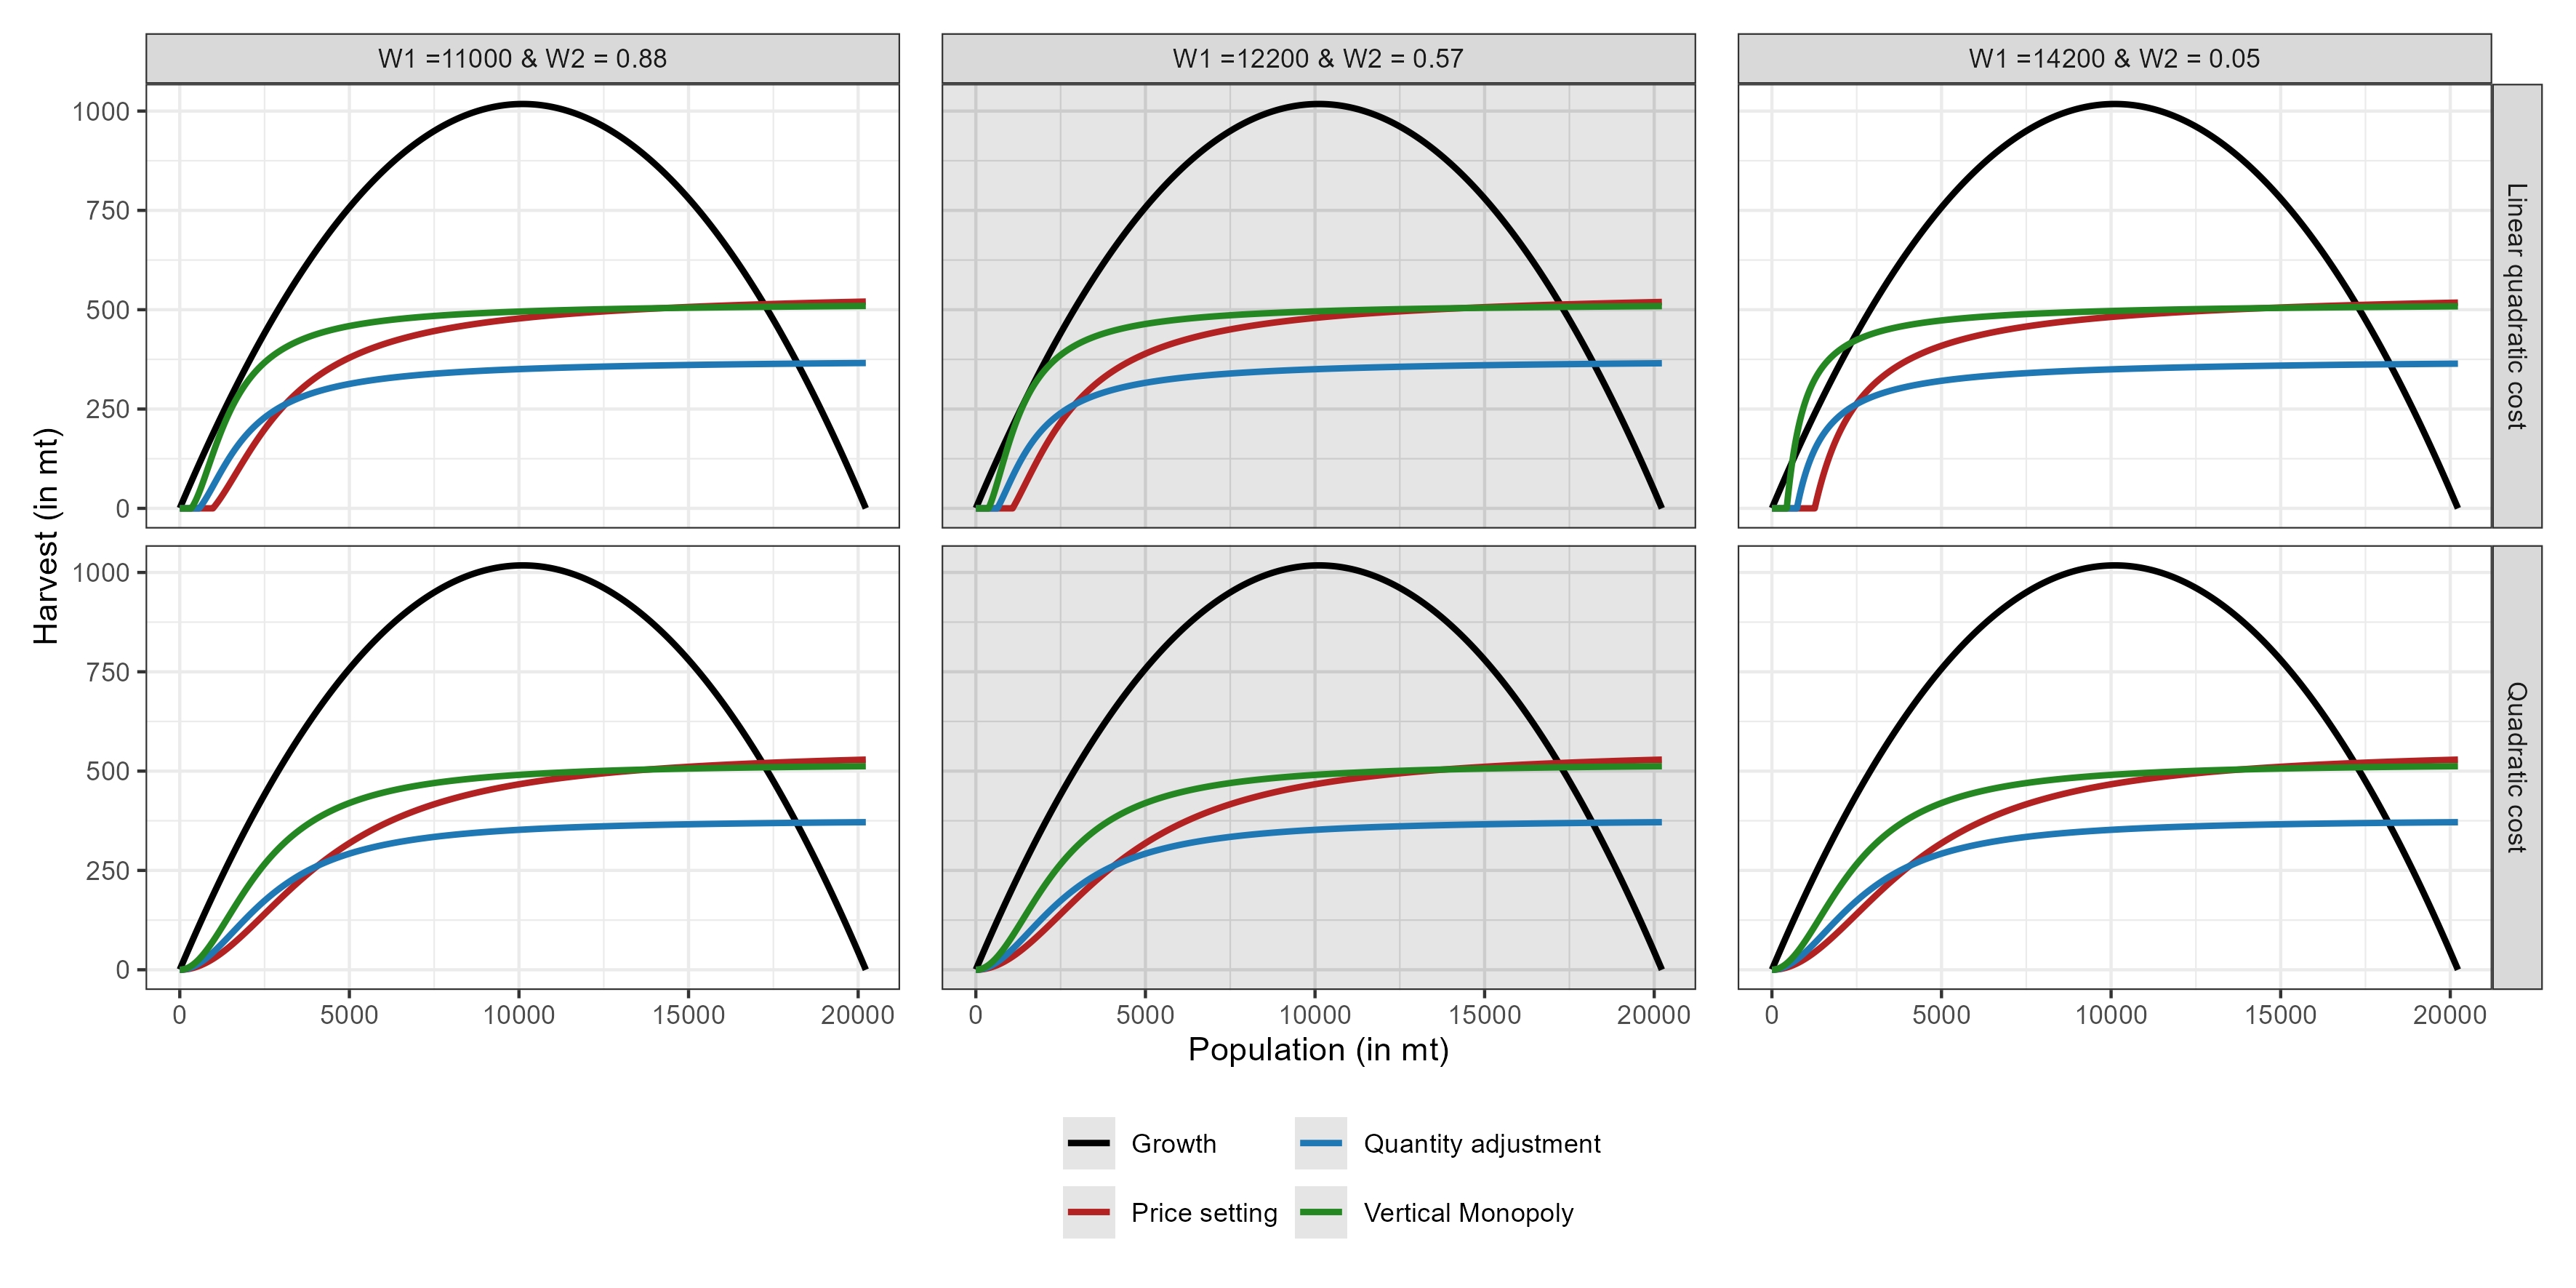
\includegraphics[width=0.85\linewidth]{figures/totoaba/figure4.png}
    \caption{ Sensitivity of equilibrium points to cost structure for wild totoaba stock}
    \subcaption*{Logistic growth function (black) for Totoaba macdonaldi wild stock biomass with intersecting colored lines representing different market structures and competitive responses. Harvest under the status quo vertical monopoly is represented by the green curve. When conservation farming is added to the monopoly scenario the trader can respond either in a mutually beneficial way by adjusting the quantity supplied given a market price (quantity adjustment, in blue). Alternatively, the trader can respond aggressively and try to set a price that undercuts the price of farmed products, resulting in increased poaching (price setting, in red). Cost parameters $W_1$ and $W_2$ correspond to the linear quadratic cost structure. In the top panel, equilibria are displayed for the linear quadratic cost, on the bottom, for a quadratic cost. On the left panel, the quadratic component is large, and vertical monopoly maintains a healthy stock. Center panel highlights the baseline scenario. In the right panel, the cost structure is close to linear. In this case, the vertical monopoly may lead to drastic stock decline.}
    \label{fig:figure5}
\end{figure}

\subsection{Farming produces conservation benefits}

While our results show that totoaba stock may remain healthy under the current monopolistic market conditions, these results are sensitive to changes in poaching costs (Figure \ref{fig:figure5}). Therefore, we ask if conservation farming can improve upon the status quo by producing a robust single high stable equilibrium point and reduced cartel profits.

We add conservation farming to the monopolist model and now have two ‘firms’ – a trader and a farmer – competing on a duopolistic market. When farming supplies legal product to end-market consumers, the demand for illegal product will fall, assuming that wild and farmed products are substitutable (an assumption we explore later). The monopolist trader can respond to competition in two ways: a mutually beneficial way by adjusting the quantity supplied given a market price (quantity adjustment), or alternatively, an aggressive way that tries to select a price that undercuts the price of farmed products (price setting). In both scenarios, the trader and farmer choose a quantity supplied simultaneously, without knowing how the other will respond. 
\\
Illegal markets are almost always characterized as competing through quantity adjustment \citep{poret_optimal_2009, flores_violence_2016}. Under the assumption that products are substitutable, it is more profitable – and therefore more likely – for both firms to compete through quantity adjustment \citep{singh_price_1984}. When goods are substitutes, if both firms restrict the quantities supplied, they both enjoy higher prices. If they flood the market, prices and profits collapse. In the case of totoaba, we find that if traders respond through quantity adjustment under the linear quadratic cost structure, then the wild stock biomass increases by $5.45\%$ (compared to a monopoly) to a steady state equilibrium of $18,220$ mt, or to $90\%$ of carrying capacity (Table \ref{fig:table}). This represents a reduction in poaching harvest of $28.27\%$ and $\$195.16$ million USD of annual lost profit to the trader.

Even if traders respond aggressively through price setting, considered a less likely response \citep{singh_price_1984} a single high equilibrium emerges (Figure \ref{fig:figure4}). Price setting is considered a much less likely response to competition because the trader would face steep profit losses. Under the high steady-state equilibrium with the linear quadratic cost structure, wild stock biomass decreases by $0.24\%$ relative to monopoly, to a steady-state equilibrium of $17,235$ mt, or to $85\%$ of carrying capacity (Table \ref{fig:table}). Although the high steady-state reflects a relatively small increase in poaching harvest by $5.85\%$, it would result in $\$313.84$ million USD of annual lost profit to the cartel, making this strategy unlikely. 

\begin{figure}[h]
    \centering
    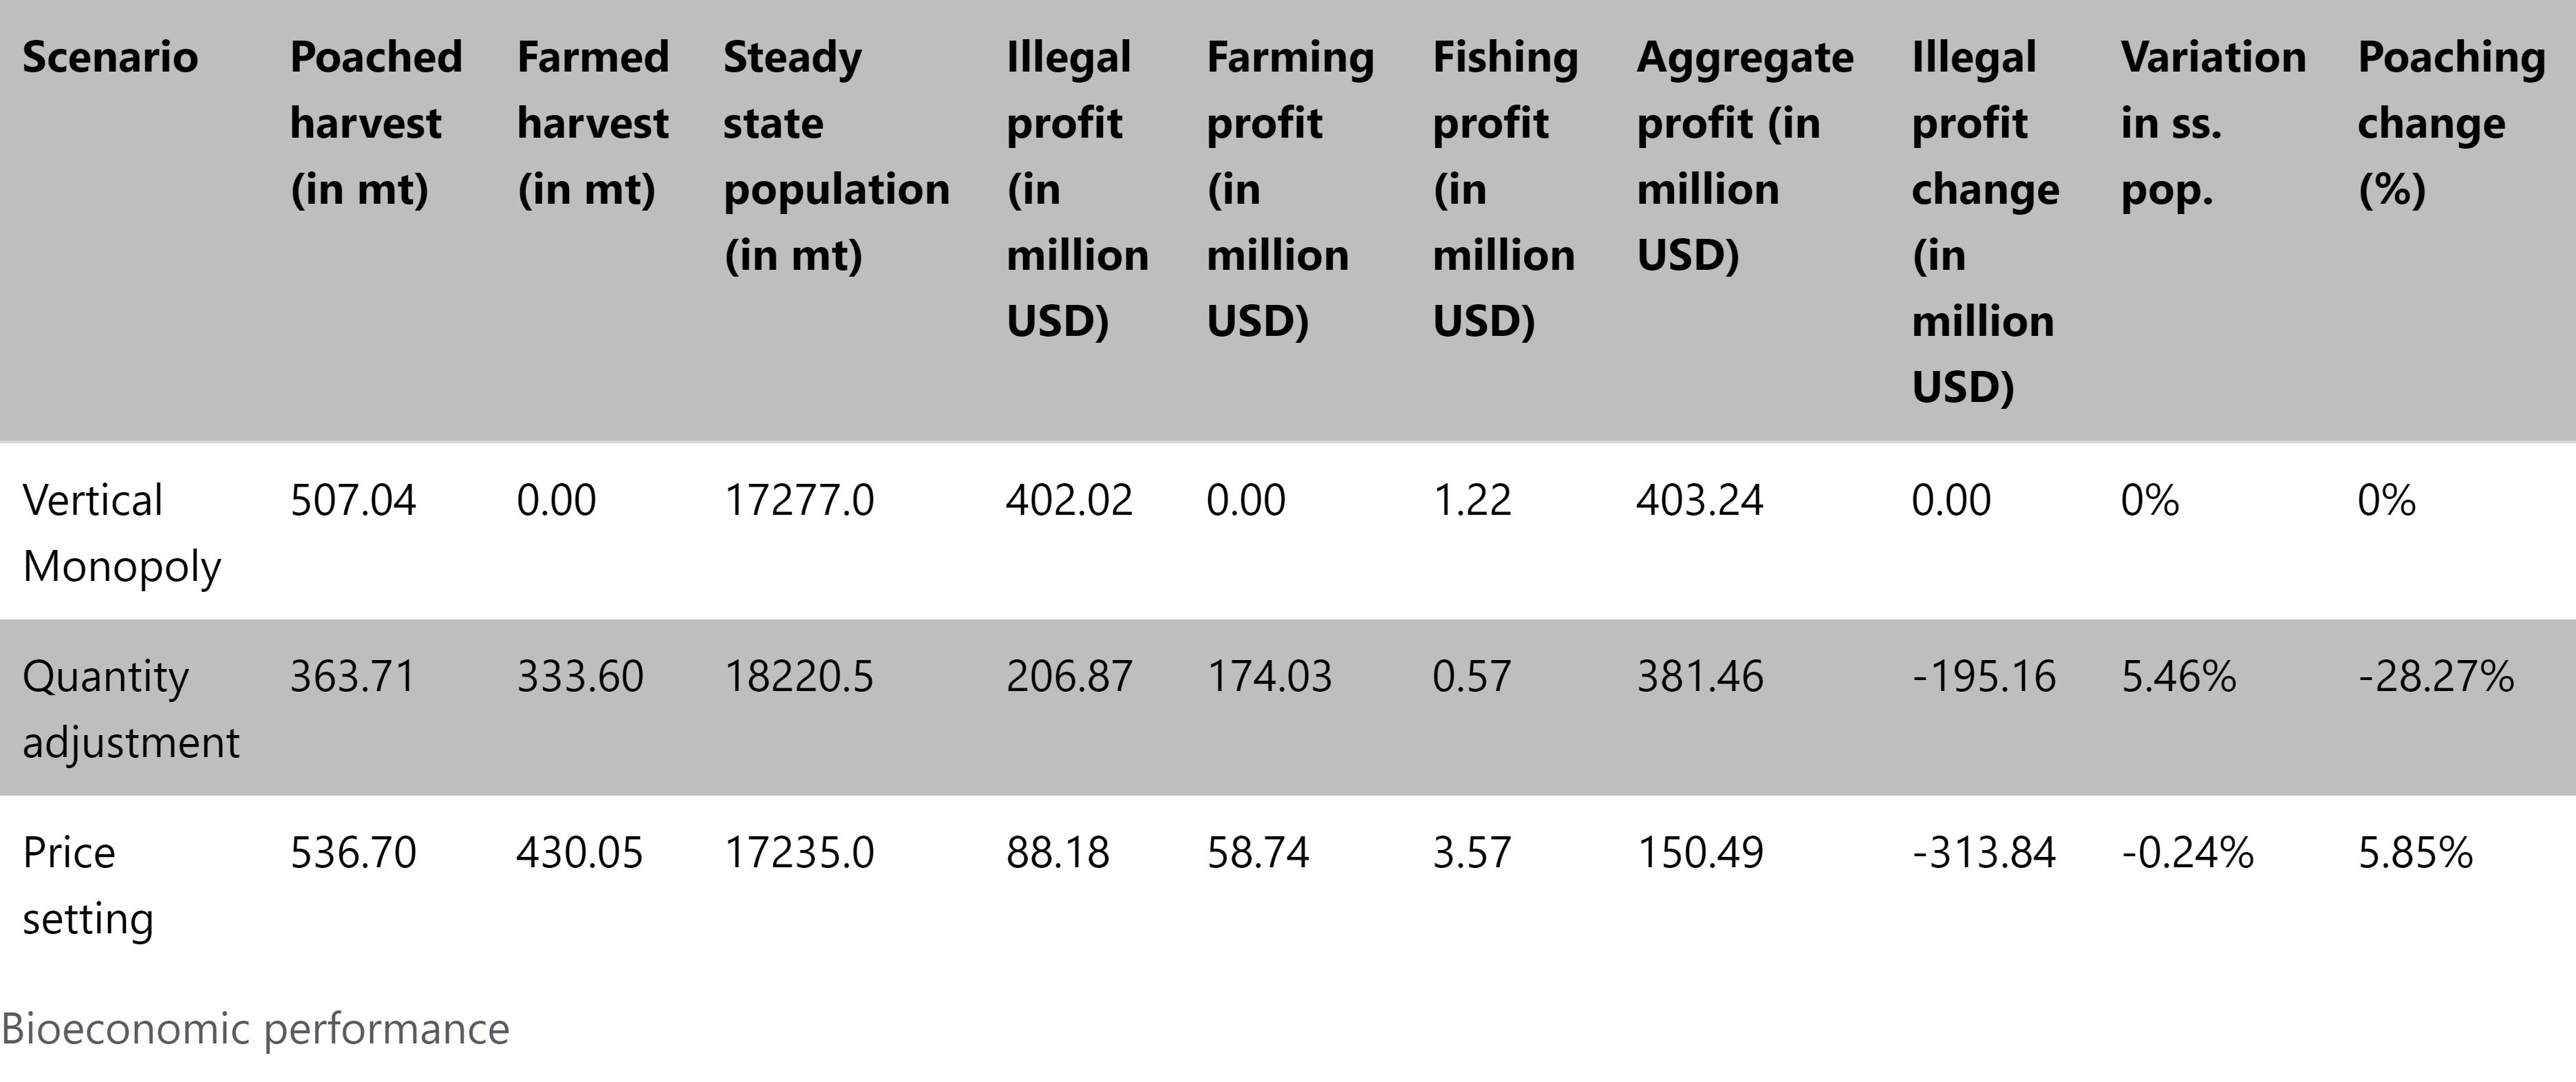
\includegraphics[width=0.85\linewidth]{figures/totoaba/bioecon_perf.png}
    \caption{Economic and ecological performance of different market regimes}
    \label{fig:table}
\end{figure}

Our current specifications for totoaba show that price setting leads to a slight increase in poaching pressure, however, we argue that price setting does not universally lead to increased poaching pressure, challenging a key conclusion from the original bioeconomic model \citep{bulte_economic_2005, damania_economics_2007}. Farming puts an upper bound on the price traders can pay to poachers in order to remain competitive. When the cost of farming becomes lower than the combined cost of poaching and trading, price-setting competition does not inevitably result in the overexploitation of the wild stock. This is because when farming costs are low, traders have an incentive to maintain large stocks by poaching less to remain competitive with farmers. This limits the price paid to poachers. On the other hand, when farming costs are large, traders have an incentive to poach more, paying a larger price to poachers while remaining competitive with the farming sector.  In the case of totoaba, species specific traits and market characteristics result in a slight increase in poaching in the price setting scenario. However, if the carrying capacity were smaller, or demand lower, the price-setting equilibrium would result in conservation benefits. 

While we focus on the effect of conservation farming on a monopolistic market structure, given that this scenario best represents the totoaba fishery today, the effect of conservation farming on market structures can be explored in different contexts. We model alternative market structures, including scenarios with multiple competing traders or multiple competing farmers, and find that if the number of farmers exceeds the number of traders, poaching levels will decline (supplementary figure \ref{fig:cournot_oligo}). Additionally, if farming is taken over by monopolists, we find that poaching is reduced and the wild population increases (supplementary figure \ref{fig:extended_cartel}).

\subsection{An effective policy space for farming.}

Our analysis provides a quantitative framework that can identify an effective policy space where all supply, demand, and market structure parameters align to ensure that conservation farming will reduce poaching, improving greatly on the original bioeconomic model and the limitations of binary qualitative approaches \citep{phelps_framework_2014,tensen_under_2016, bulte_economic_2005, damania_economics_2007, challender_evaluating_2019}. This bioeconomic model allows researchers to quantify: (a) how much cheaper farming must be relative to poaching to be competitive; (b) how much of a demand increase can be absorbed by farming; and (c) how substitutable must wildlife products be for farmed products to displace wild products. Critically, we also explore how the interaction between these factors may affect outcomes. We explore how sensitive the results are for totoaba, offering general and totoaba-specific policy solutions to help ensure that conservation farming remains in the effective policy space.

We find that the cost of conservation farming for totoaba can be high and still competitive with poaching, but this is contingent on the cost for traders also being high (supplementary figure \ref{fig:c_and_v}). Traders inherently rely on poachers to obtain totoaba, and if farming is expensive this forces traders to pay poachers higher prices. If traders compete with poachers under the more likely quantity adjustment response, the population remains healthy, even increasing by nearly $6\%$ from the monopoly steady state. However, if traders compete with farmers by price setting, the low prices paid to poachers can incentivize poachers to increase fishing pressure in order to maintain payouts. This can lead to a decrease in the wild population biomass modestly by $0.24\%$ from the monopoly steady state. Policymakers can support farming success by subsidizing farming to keep the cost low while maintaining enforcement to keep the cost of poaching high (for totoaba this includes marine patrols, fisheries closures, and gillnet bans). To mitigate the possibility of stock decline under the less-likely price-setting response, we identify that maintaining conservation farming below $\$77,339$ USD per mt of totoaba (amounting to a $14\%$ subsidy on unit production cost) will prevent any increase in poaching pressure under either competitive response, assuming no effect of law enforcement in our baseline model.


\begin{figure}[h]
    \centering
    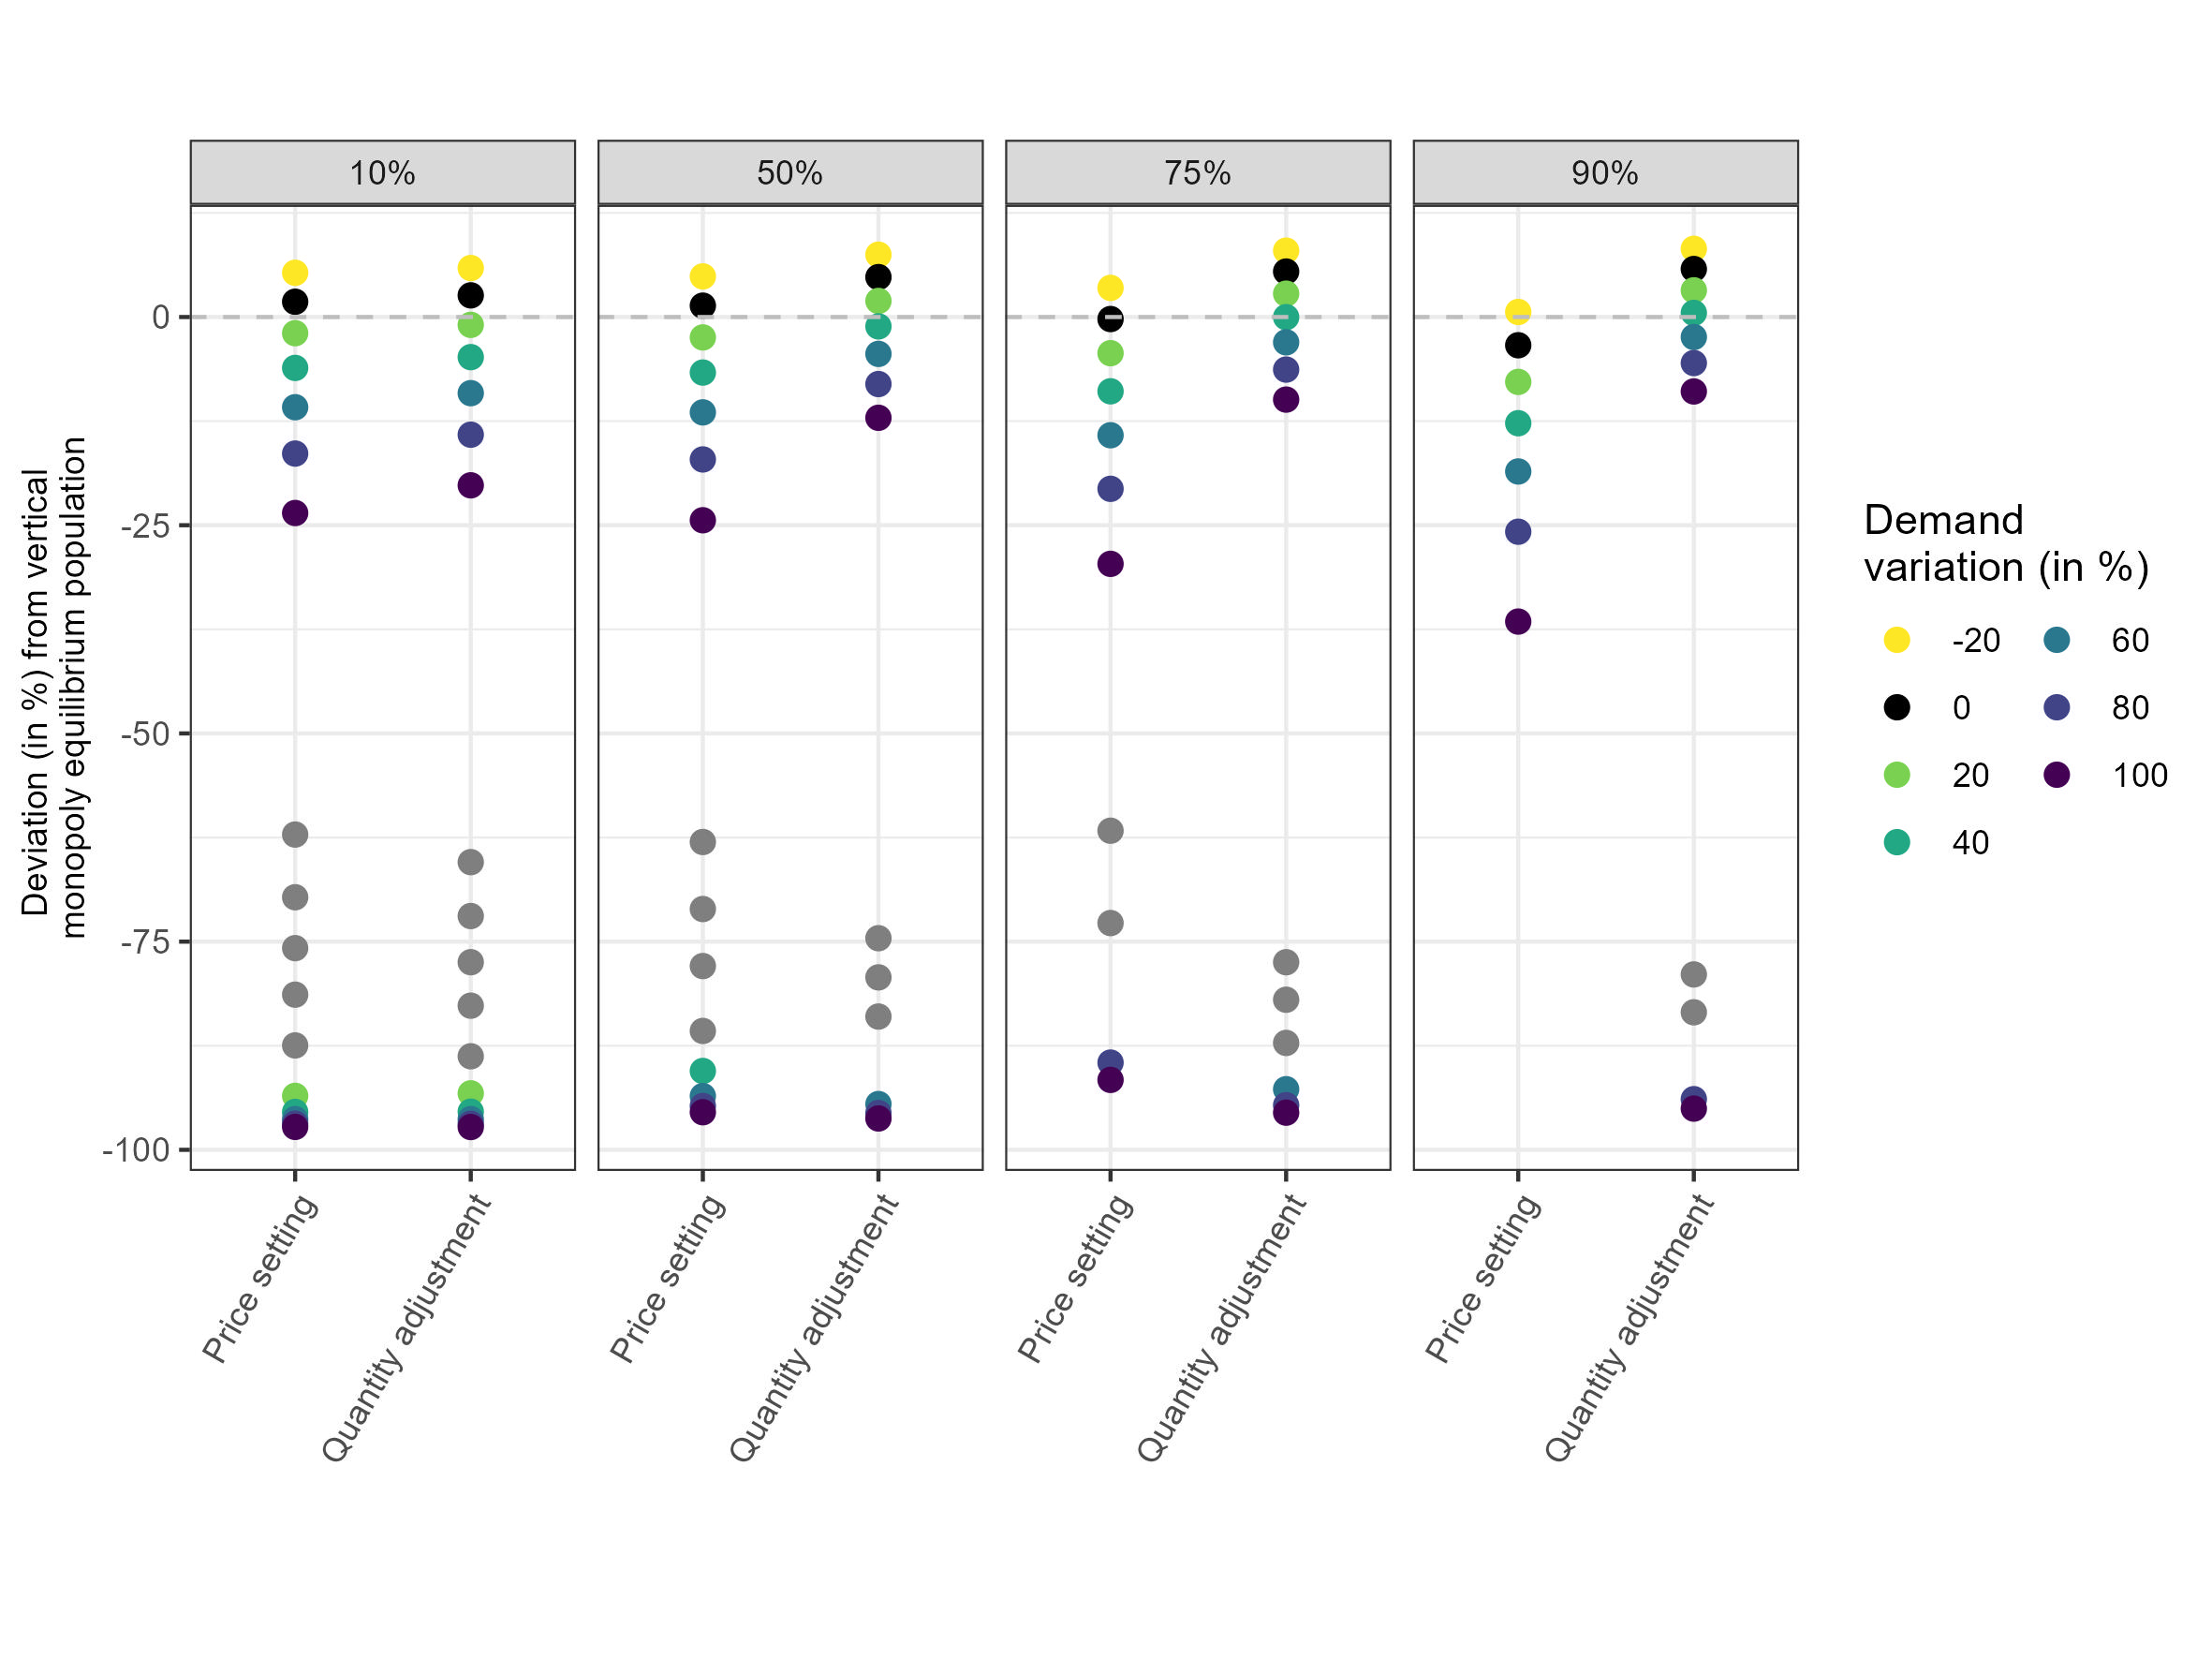
\includegraphics[width=0.85\linewidth]{figures/totoaba/Figure5.jpg}
    \caption{Interaction between substitutability and demand under duopolistic competition}
    \subcaption*{Each panel represents a different substitutability between farmed and wild product: large ($90\%$ substitutability), baseline ($75\%$), medium ($50\%$ substitutability), and low (10\% substitutability). Our baseline results are in the $75\%$ substitutability case, with zero demand variation (black dots) When conservation farming is added to the monopoly scenario the trader can respond aggressively and try to set a price that undercuts the price of farmed products (price setting), alternatively the trader can respond in a mutually beneficial way by adjusting the quantity supplied given a market price (quantity adjustment). We simulate a change in end-market demand ranging from a reduction in demand by $20\%$ to an increase in demand up to $100\%$, in increments of $20\%$. One, two, or three potential equilibria can emerge. Where three equilibrium points emerge, we color only the high and low stable equilibria (unstable equilibria are indicated in gray). The dotted horizontal lines indicate the status quo monopoly equilibrium population (in the absence of conservation farming). Points closer to 0 represent a high stable equilibrium point, whereas points closer to $-100$ represent a population collapse stable equilibrium point.}
    \label{fig:figure6}
\end{figure}

Our results confirm that high substitutability is critical to conservation farming success and leads to larger conservation benefits in the quantity-setting equilibrium, under the assumption that demand remains stable (Figure \ref{fig:figure6}). Fish swim bladders have a wide variety of uses and values, and it is possible that farmed totoaba swim bladders may enter into these different product streams \citep{sadovy_de_mitcheson_emerging_2019}. In the case of no substitutability, two separate, non-competitive markets emerge. In this scenario the status quo is maintained, both firms set high prices, and traders continue to operate as a monopoly because farmed product does not compete with wild product. At the other extreme, in the case of perfect substitutability, consumers prefer the cheaper option without any preference of source. This increases the intensity of potential price-setting competition between firms and further depletes the stock in this case. To comply with CITES captive breeding guidelines totoaba must be identified as farmed \citep{cites_additional_2019}, and distinguishing between products to meet regulatory obligations can artificially lower substitutability. Outcomes vary under intermediate states of substitutability. For low to medium substitutability (i.e., $10-50\%$) traders and farmers are still likely to limit quantity: undercutting a competitor would yield significant profit losses. For high substitutability (i.e., $90\%$) there is an incentive to compete for market control either by price setting or quantity adjustment, which reflects our main results. 

The value of totoaba swim bladder is tied to rarity, and while demand evolution is an open empirical question, we test the sensitivity of our results to simultaneous changes in demand and substitutability (Figure \ref{fig:figure6}). Totoaba swim bladder purchases are ‘conspicuous consumption,’ luxury products commonly purchased for social status and speculative investing by wealthy consumers \citep{sadovy_de_mitcheson_emerging_2019, veblen_theory_2023}. A decrease in swim bladder price resulting from conservation farming may actually undermine the desirability of totoaba swim bladders in Chinese end markets, given that the high monetary value is linked to high social status \citep{jinkins_conspicuous_2016}. However, some increase in demand may be expected if a legal product becomes available, as law-abiding consumers will be more likely to purchase wildlife products when those products are traded and purchased legally \citep{phelps_framework_2014}. Under our high substitutability assumption ($75\%$), competition through quantity adjustment can withstand a $40\%$ increase in demand, whereas competition through price setting is not robust to demand increases. For price setting, a demand increase of $40\%$ would cause the equilibrium population to decrease by $10\%$ from the monopoly status quo, increasing poaching by $216$ mt. 

There is a much higher threat to the wild population if demand increases under low to medium substitutability (i.e. $10-50\%$), given that this additional demand cannot be fully met by farmed product (Figure \ref{fig:figure6}). In the best-case and most likely scenario, medium substitutability ($50\%$) can meet a $20\%$ increase in demand if competition occurs through quantity adjustment, although uncertain outcomes (e.g. high and low steady states) start to emerge if demand increases by $60\%$ or more. In the worst-case scenario, if competition occurs through price setting and products have medium substitutability ($50\%$), any increase in demand reduces the wild population from the status quo. While increases in demand of $20-40\%$ still produce a single high equilibrium point, the population size is lower than under monopoly. Furthermore, if demand increases beyond $80\%$, uncertain outcomes emerge, with the wild population either stabilizing at a high equilibrium point ($14,322$ mt in the price setting scenario; $15,886$ mt in the quantity adjustment scenario) or being pushed to a low equilibrium point (ranging from $763$ mt in the quantity adjustment scenario; $909$ mt in the price setting scenario). We recommend that stated preference investigations on wild versus farmed product should be undertaken in Chinese end-markets and that these investigations include questions focused on perceived social status benefit and legality \citep{hinsley_wild_2020}. 

\section{Conclusion}
Our results show that conservation farming presents a potentially high reward intervention. If traders respond to competition from farming by quantity adjustment, the wild totoaba stock is predicted to increase by $5.45\%$ relative to the status quo monopoly, to a high stable biomass of $18,220$ mt ($90\%$ of carrying capacity). In addition to improving the totoaba wild stock, this quantity adjustment response will decrease poaching by $28.27\%$ relative to the status quo. If traders respond by price setting, the wild stock biomass decreases by less than $1\%$ to a high stable biomass of $17,235$ mt ($85\%$ of carrying capacity). Economic theory concludes that quantity adjustment is the more likely outcome because restricting quantities allows both farmers and traders to collect higher profits \citep{singh_price_1984}. Conservation farming presents a more robust outcome to the status quo monopoly market structure (where a single trader dominates the market), as the wild totoaba reaches either a low or high stable equilibrium biomass depending on the poaching cost structure. We find that if products have high substitutability they are more likely to maintain a high stable equilibrium. Further, under a quantity adjustment response, highly substitutable products can better maintain this high stable equilibrium for demand increases up to $40\%$. Our results are sensitive to changes in substitutability and increases in demand, therefore we encourage a thorough understanding of end-market demand before implementing conservation farming for totoaba.

We revive an existing bioeconomic model and reach different and optimistic conclusions about the potential for conservation farming to reduce poaching and maintain a healthy wild population. We provide a novel framework to objectively assess the potential effects of farming by grounding our analysis in detailed species ecology and market data. Furthermore, our approach provides a rigorous alternative to existing qualitative frameworks that are unable to analyze the interaction between multiple variables. While our analysis focuses on totoaba, the bioeconomic model is flexible and can be applied more broadly to other species and contexts to examine the effect of conservation farming on a wild population. 


%\section{Methods}

\subsubsection*{Acknowledgements}
We thank Mark Buntaine, Chris Costello, and Lauriane Mouysset for helpful comments and feedback on the manuscript, as well as members of the Costello research group. J.M.L acknowledges funding from the Daniel and Dianne Vapnek Fisheries Management Fellowship, the Schmidt Family Foundation Research Accelerator Award as well as from the National Sciences and Engineering Research Council of Canada (NSERC) Postgraduate Scholarship. M.C.-R. acknowledges funding from the Latin American Fisheries Fellowship. 

\section*{Contributions and data availability}

J.M.L and S.J contributed to this work equally. J.M.L., S.J., M.C-R., G.M.G., M.A.C-M., E.A-B, and S.D.G. contributed to writing the manuscript. J.M.L., S.J., A.S., and S.D.G. contributed to study conception and design. All authors contributed to data acquisition and analysis. All authors approve of the submitted manuscript.
\\
The data that support the findings of this study are available  \href{https://doi.org/10.17605/OSF.IO/6Y8CQ}{here}
\\
The code used for this study is publicly available on \href{https://github.com/julawson/conservation_farming_totoaba}{Github} and \href{https://doi.org/10.17605/OSF.IO/6Y8CQ}{archived here}


	\clearpage
	
	\begin{appendices}
	\renewcommand{\thesection}{3.\Alph{section}}
	\renewcommand{\thefigure}{3.\Alph{section}.\Alph{figure}}
	\renewcommand{\thetable}{3.\Alph{section}.\Alph{table}}
	\counterwithin{figure}{section}
	\counterwithin{table}{section}
	\section{A theoretical model of poachers, traders, and farmers}

Our framework follows [19], with a poaching cost structure adapted to fisheries. The model develops a three-stage dynamic, game theoretic, bioeconomic model. The value chain for poached animal products comprises poachers, middlemen traders, and end markets. As a small number of actors characterizes many wildlife markets, the model features a vertical monopoly and looks at the consequences on wildlife population stocks of the introduction of a farmed substitute. In this setting, farmers compete on end markets with traders in quantity and price. In the original model, price competition unambiguously results in larger harvests than in the vertical monopoly case. Therefore, while quantity competition reduces poaching, the threat of a population collapse in the price-setting case should warrant a cautious approach to conservation farming. We argue that this conclusion is erroneous, as the intricacies of imperfect substitutability and market dynamics have not been properly accounted for in the original model. As a matter of fact, standard economic intuition regarding price-setting competition in the homogeneous goods case does not directly apply here, as fishing costs rise as the stock decreases, limiting the ability of the trader to flood the market. We show that scenarios exist where any type of competition unambiguously leads to positive conservation outcomes, i.e, reduced poaching and larger steady-state stocks. We amend the original results and use this model for simulation. 

First, poachers illegally harvest wildlife resources. Second, they sell their catch to a monopsonistic buyer. Third, the buyer sells catches on a monopolistic market, which is not accessible to poachers. We label this value chain 'vertical monopoly' as a reference case. We then look at the impact of introducing a competitor on the end market, the farming sector. 

%For comparison, we look at the impact of conservation farming on several other market structures. We model an open-access fishery, where the middlemen traders disappear and poachers sell their catch on a perfectly competitive market. As Damania and Bulte (19), we model the case where a middleman trader exists and sells the catch on a perfectly competitive market. 

%\subsection{The open access fishery model}

%First, consider an open-access fishery, where fishermen optimally determine effort to maximize their profits and sell their catch without an intermediary.


\subsection{Entry in the fishery and poaching supply}
We denote the fishing effort by $E$, which is measured in the number of vessel trips. Entry in the poaching sector, $\dot{E}$, is a function of payoff and an adjustment parameter.  Harvest, $q$, follows the Gordon-Schaefer  dynamic biomass model  $q = \sigma x E$, with $\sigma$ the (stock-independent) catchability coefficient, and $E$, effort
%\cite{Clark}
The payoff is determined by the price paid to the poachers $s$ minus the cost of effort. We adopt a disagregated view of the fishery, and consider increasing marginal costs of effort, as individuals have to be attracted from other activities with increasing opportunity costs. To account for energy costs, we derive a modified version of this model using a linear-quadratic cost function (see [37, 53]). Entry happens as long as the profit of the marginal poacher is positive : 
\begin{equation}
    \dot{E}= \eta \frac{d\Pi}{dE} = \eta \frac{d}{dE}\left[ sq-W_1 * E - W_2E^2\right]
\end{equation}
%reach a closed form solution for the optimal $E$ such that it increases in the price paid to poachers and stock.

The resource stock biomass $x$ follows a logistic growth curve and is harvested. Overall, the dynamics are: 
\begin{equation}
    \dot{x} = g(x) - q = rx\left(1 - \frac{x}{K}\right) - \sigma x E
    \label{eq:growth}
\end{equation}
Where $r$ is the intrinsic population growth rate,  and $K$ is the carrying capacity. 

Fishermen enter the fishery as long as the marginal profit from selling to traders along the vertical value chain is positive. As the resource is in open access from the fishermen poachers maximize their instantaneous profit with respect to effort. The optimal effort and aggregate supply of poached fish is:
\begin{align}
    \frac{d \Pi}{d E} = 0
    \Rightarrow & E^* = \max\left( 0, \frac{s \sigma x  -W_1}{2W_2} \right)\\
    \Rightarrow & q^* = \max\left(0, \frac{s\sigma^2 x^2 - W_1\sigma x}{2 W_2}\right)
    \label{eq:poachers_supply}
\end{align}
Given the linear quadratic nature of the costs, there is no effort or catch for low stock levels and/or low prices. Effort and catch increase with the price paid to poachers, $s$.


%The steady state is defined by $\dot{E}=\dot{x}=0$. Plugging the optimal effort in the harvest function yields the supply of the poaching sector and steady state stock in \textbf{open acces}:

%\begin{align}
%   \text{Poaching in} \text{ \textbf{open access} : }
%   q^W =& \sigma  x E = \frac{s \sigma^2 x^2}{2W} \\
%    \label{eq:poachers_supply}
%    \text{Steady state stock} \text{ in \textbf{open access } : }
%    x^*=&\frac{2WrK}{s\sigma^2K + 2Wr}
%\end{align}

%Notice that if prices drop, harvest decreases, and the steady state stock increases.


%\subsection{Wildlife commodity traders as price takers}
%In this part of the model, we introduce a new actor: a wildlife trader buys totoaba from poachers. 

%The trader maximizes profit by determining the price paid to poachers, taking market prices for totoaba as given. Recall that the quantity produced, for the marginal unit of effort to not earn rent is $q^W$. Using $c$ as a transportation and transaction cost : 
%\begin{equation*}
%    \Pi^W= Pq^W - sq^W = (P  -c - s)\frac{s\sigma^2 x^2}{2W}
%\end{equation*}
%We assume the inverse demand function is linear : 
%\begin{equation}
%    P^m = \alpha^m - \beta^m q^W
%\label{eq:inv_demand_monop}
%\end{equation}

%Using $q^W$ and optimizing with respect to $s$ yields $s^*=\frac{P-c}{2}$, and the poaching function and steady state stock \textbf{when wildlife commodity traders are price takers}  : 
%\begin{align}
%    \text{Poaching when the }  \text{\textbf{trader is price taker} : }
%    q_P^W&=\frac{(P-c)\sigma^2x^2}{4W} = \frac{(\alpha^m -c)\sigma^2 x^2}{4W + \beta^m \sigma^2 x^2}\\
%    \label{eq:poaching_sup}
%    \text{Steady state stock when the}  \text{\textbf{trader is price taker} : }
%    x^* &= \frac{4WrK}{P\sigma^2K + 4Wr}
%\end{align}

%As in Damania and Bulte (19):
%\begin{displayquote}
%    \textbf{Lemma 1:} \textit{Ceteris paribus, the introduction of farmed animal products will decrease the level of poaching relative to that which occurs in the absence of farming for any given wildlife stock if commodity traders are price takers. As a result, the steady-state population increases.}
%\end{displayquote}
%If farming is introduced with sufficient quantity, it is expected that (i) market prices will drop. In this case, 
%If (i) farming implies that market price goes down, then (ii) $\frac{dq^W_P}{dP}>0$ implies that poaching will decrease. Lower poaching levels translate to larger stocks, as $\frac{dx^*}{dP}<0$.

\subsection{Traders as vertical monopolists, without farming}
We introduce a trader who has market power on the end-market (monopoly) and on the primary market, making it a \enquote{vertical monopoly}. The trader has to set price $s$ on the primary market to clear the poaching market. On the end market, we assume the trader faces a linear inverse demand : 
\begin{equation}
    P^m = \alpha^m - \beta^m q^W
\label{eq:inv_demand_monop}
\end{equation}

Trading an illegal commodity incurs transaction costs $c$. Hence, the monopoly profit can be written as : 
\begin{equation}
    \Pi^m = (\alpha^m - \beta^mq^W - c -s )q^W
    \label{eq:profit_monop}
\end{equation}
The optimal level of output is : 
\begin{equation}
    \Tilde{q_m^W}=\frac{\alpha^m - c - s}{2\beta^m}
    \label{eq:monop}
\end{equation}

Using the poachers' supply, it must be that in equilibrium, the supply of the monopolist trader equals the supply of the poachers. The price paid to poachers $s$ balances supply and demand (consistent with equation 13 in \cite{damania_economics_2007}). Substituting $s^*$ into equation \ref{eq:monop} yields the quantities of poached product in the vertical monopoly scenario : 
\begin{align}
    \text{Price paid to poachers :} s^*_m(x) &= \frac{W_2 (\alpha_m -c) + \beta^m (W_1 \sigma x) }{ \sigma^2 x^2 \beta^m + W_2 }\\
        \text{Poaching : } q^*_m(x) &=\frac{\sigma^2 x^2 (\alpha_m - c) - W_1 \sigma x}{2(\sigma^2 x^2 \beta^m +W_2)}
    \label{eq:harvest_monop}
\end{align}
First, note that equation \ref{eq:harvest_monop} is consistent with equation 14 in \cite{damania_economics_2007}, as the limiting case where $W_1= 0$ and $W_2 = W$. 
%Second, note that harvest increases with the stock at a decreasing rate
%\\\\
%In the \textbf{vertical monopoly equilibrium}:
%\begin{align}
%    \text{Price paid to poachers : } s^*_m(x) &= \frac{(\alpha^m - c)W}{\beta^m \sigma^2x^2+W} \\
%    \text{Poaching : }q^{W*}_m &= \frac{(\alpha^m-c)\sigma^2 x^2}{2\beta^m \sigma^2 x^2 + 2W}
%    \label{eq:harvest_monop}
%\end{align}
 
%Lemma 2 summarizes these findings.

%\begin{displayquote}
%    \textbf{Lemma 2:} \textit{For low stock values, harvest when the trader is price taker is lower than when the trader is monopolistic. For larger stock values, it is unambiguously larger than in the monopolistic case.}
%\end{displayquote}
%\paragraph{Proof: }Compare the harvest functions in the case where the trader is a price taker and when it is a price maker : 
%\begin{align*}
%    q^W_m &\leq q^W_P \\
%    \Rightarrow \frac{(\alpha^m - c) \sigma^2 x^2}{2\beta^m \sigma^2x^2+2W}&\leq \frac{(\alpha^m - c)\sigma^2 x^2}{4W+\beta^m \sigma^2 x^2}\\
%    \Rightarrow \sqrt{\frac{2W}{\beta^m\sigma^2}} &= \Tilde{x}\leq x
%\end{align*}
%fies a threshold value $\Tilde{x}$ for the ranking of harvest functions, which is independent of biological parameters. This lemma only establishes the ranking of harvest functions but does not establish steady-state properties. In determining equilibrium properties, the properties of the growth function will determine the ranking of the steady states. We go back to this point in section \ref{section:steadystates}. 
\subsection{Captive breeding, imperfect competition and conservation}
In this part of the model, a farmer can grow and sell totoaba. The theoretical model focuses on the duopolistic competition between the two actors on the end market for totoaba. As products are strategic substitutes, it is natural to investigate the case where Cournot competition arises. Indeed, when products are substitutes, each firm tries to maximize its residual demand (25). Nonetheless, given the asymmetric nature of costs, we also investigate Bertrand competition, as \cite{damania_economics_2007}.

\subsubsection{Introducing aquaculture}
\label{subsec:aquaculture}
The aquaculture farm needs to determine the optimal harvest age, based on the intrinsic growth rate in the pen, and expected prices. A sizeable literature has shown that rotation time is invariant to market structure in forestry applications \citep{faustmann1849, mitra_faustmann_1986} although quantities can be modified. The optimal rotation literature confirms the existence of a Faustmann rotation, where a set of $T^*$ pens are equally distributed among each age class (1 pen per age class until $T^*$). While it is arguably unrealistic to expect this structure for an inherited forest, it is reasonable to assume that a farm would \textit{ex-ante} determine this rotation period given the expected price schedule over time. We assume that the aquaculture farm aims at producing a product that is as similar as possible from a biophysical stand-point and thus determines $T^*$.
As we consider a stationary demand function, one can write the farming problem as a linear profit maximization problem, where the unit cost of production equals the capitalized sum of annual average variable costs over $T^*$ periods. 
%\cite{Guttormen} : 51
% Mitra : 52
% Crabbé : 53
Therefore, we assume that an aquaculture firm can raise totoaba at cost $v$ and sell it to the market: 
\begin{equation}
    \Pi^F = (P^F- v)q^F
    \label{eq:profit_aquaculture}
\end{equation}
With $v$ the unit cost per ton of totoaba, corresponding to the capitalized sum of annual costs. 

\subsubsection{Utility maximization and demand functions}
Upon the introduction of farmed goods, the inverse demand functions change. 
We use a model consistent with Singh and Vives (25), where a representative consumer maximizes  a quadratic and strictly concave utility function subject to prices: 
\begin{equation}
    \max_{q^W, q^F}V = \alpha^W q^W + \alpha^F q^F - \left(\frac{\beta^W (q^W)^2 + 2\gamma q^W q^F +\beta^F (q^F)^2}{2}\right) - p^Wq^W - p^Fq^F
\end{equation}

Two inverse demand functions emerge, that the traders and farmers face : 
\begin{align}
P^W &= \alpha^W- \beta^W q^W - \gamma q^F \label{eq:demand_wild}\\
P^F &= \alpha^F
 - \beta^F q^F - \gamma q^W \label{eq:demand_farmed}
\end{align}
Where $W, F$ refers to wild and farmed. We assume $\gamma>0$ e.g that goods are substitutes. When $\alpha_W = \alpha^F$ and $\beta^W = \beta^F = \gamma$, the goods are perfect substitutes. When $\alpha^F = \alpha^W$, but $\beta^F \neq \gamma$ or $\beta^W \neq \gamma$,  $\frac{\gamma^2}{\beta^W \beta^F}$ measures the degree of product differentiation. 


Rearrange the initial inverse demand functions into direct demand functions:
\begin{align}
    q^W &= a^W - b^W P^W + e P^F\\
    q^F &= a^F - b^F P^F + eP^W
\end{align}
With $a^i = \frac{\alpha^i \beta^j - \alpha^j\gamma}{\beta^i \beta^j - \gamma^2}$, $b^i = \frac{\beta^j}{\beta^j\beta^i - \gamma^2}$ and $e = \frac{\gamma}{\beta^i\beta^j - \gamma^2}$
\subsubsection{Cournot competition in the retail market}

Assume that the two firms compete by setting their quantities. We solve the multi-stage game using backward induction. First, we derive the supply function resulting from Cournot competition. Second, we find the price paid to poachers so that the quantities supplied by the traders on the end market equal the quantities supplied by poachers. 

Taking the inverse demand functions and plugging them into the profit functions:
\begin{align*}
    \Pi^F& = (\alpha^F - \beta^F q^F - \gamma q^W - v)q^F\\
    \Pi^W &= (\alpha^W - \beta^W q^W - \gamma q^F - s - c)q^W
\end{align*}
In a Cournot equilibrium, each firm takes its competitor's quantity as given, and picks optimal reaction functions.

Solving for the Nash equilibrium using reaction functions, each firm supplies: 
\begin{align}
    \Tilde{q^W_c} &= \frac{2\beta^F(\alpha^W - (s+c)) - \gamma(\alpha^W - v)}{4\beta^W\beta^F - \gamma^2}\\
    \Tilde{q^F_c}&= \frac{2\beta^W(\alpha^F-v)-\gamma(\alpha^W - s -c)}{4\beta^W\beta^F-\gamma^2}
\end{align}
Now, we find the equilibrium price paid to poachers for each unit of totoaba $s^{*}_C(x)$ by equating $\Tilde{q^W_c}$ and $q^W$, and find the Nash equilibrium supply functions. 
\\\\
In the Cournot equilibrium:
%\begin{align} % with quadratic costs
%    \text{Price paid to poachers : }s^*_C(x) &= \frac{2W[2\beta^F(\alpha^W - c) - \gamma(\alpha^F-v)]}{(4\beta^F\beta^W -\gamma^2)\sigma^2 x^2 + 4W\beta^F} 
%    \label{eq:s_c}\\
%    \text{Poaching: }q^{W*}_C  & =\frac{\sigma^2 x^2[2\beta^F(\alpha^W - c) - \gamma(\alpha^F - v)]}{(4\beta^W\beta^F - \gamma^2)\sigma^2 x^2 + 4W\beta^F}\\
%     \text{Farming : }q^{F*}_C &=\frac{\sigma^2 x^2[2\beta^W(\alpha^F-v) - \gamma(\alpha^W - c)] + 2W(a^F-v)}{(4\beta^F\beta^W - \gamma^2)\sigma^2 x^2 + 4W\beta^F}
%\end{align}
\begin{align}
    \text{Price paid to poachers: } s_C^*(x) &= \frac{2 W_2(2\beta^F(\alpha^W - c) - \gamma(\alpha^F - v)) + W_1 \sigma x(4\beta^F\beta^W - \gamma^2)}{4W_2 \beta^F + \sigma^2 x^2(4\beta^F\beta^W -\gamma^2)} \label{eq:price_poachers_cournot}\\
    \text{Poaching : } q^{W*}_C(x) &= \frac{\sigma^2 x^2(2\beta^F(\alpha^W -c) - \gamma(\alpha^F - v)) - 2\beta^F W_1 \sigma x}{4 W_2 \beta^F + \sigma^2 x^2(4\beta^W \beta^F - \gamma^2)}
    \label{eq:poaching_cournot}
     %\text{Farming : }q^{F*}_C &=\frac{\sigma^2 x^2[2\beta^W(\alpha^F-v) - \gamma(\alpha^W - c)] + 2W(a^F-v)}{(4\beta^F\beta^W - \gamma^2)\sigma^2 x^2 + 4W\beta^F}
\end{align}
First, including a linear component for energy in the poaching cost significantly raises the price paid to poachers (when $W_1>0$).
Second, poaching decreases with the degree of substitutability between farmed and wild products ($\gamma$), and increases with the production cost of farmed products $v$. On the other hand, it increases with demand for the wild product $\alpha^W$.
For low stock values, poaching can be null since the production costs increase as stocks diminish. In the polar quadratic cost case (e.g. $W1 = 0$), our results differ from \cite{damania_economics_2007} by a magnitude effect. Nonetheless, the results stand : 
\begin{displayquote}
    \textbf{Lemma 1}:  \textit{Assume the market is large, i.e., the residual demand for large stock levels is large enough. For any given wildlife stock, poaching levels in equilibrium with captive breeding will be lower than those without captive breeding, if the introduction of captive-bred animal products has no impact on the parameters of the original inverse demand function for wild animal products.}
\end{displayquote}
See Appendix \ref{section:AppendixB}. for proof of Lemma 1

\subsubsection{Bertrand competition in the retail market}
\paragraph{Interior solution:} the two firms compete by setting their prices. This section investigates a potential interior equilibrium, where both producers operate on the market. 

Using demand functions instead of inverse demand functions: 
\begin{align*}
    q^F = a^F - b^FP^F + e P^W\\
    q^W = a^W - b^WP^W + e P^f
\end{align*}
With $a^i = \frac{\alpha^i \beta^j - \alpha^j \gamma}{\beta^i\beta^j - \gamma^2}$, $b^i = \frac{\beta^j}{\beta^j \beta^i - \gamma^2}$ and $e=\frac{\gamma}{\beta^i \beta^j - \gamma^2}$
\\\\
Firms set their prices. The Bertrand profit equations are : 
\begin{align*}
    \Pi^F = (P^F - v)q^F = (P^F - v)(a^F - b^F P^F + e P^W)\\
    \Pi^W = (P^W - (s+c))q^W = (P^W - (s+c))(a^W - b^W P^W + e P^F)
\end{align*}
Solving for the reaction functions : 
\begin{align}
    r^F(P^W) &= \frac{a^F + b^F v + e P^W}{2b^F}\\
    r^W(P^F) &= \frac{a^W + b^W(s+c) + e P^F}{2b^W}
\label{eq:rf_bertrand}
\end{align}
Finding the interior solution for the Nash Equilibrium :
\begin{align*}
    P^F_B &= \frac{2b^W(a^F + vb^F) + e(a^W + b^W(s+c))}{4b^Fb^W - e^2}\\
    P^W_B &= \frac{2b^F(a^W+ b^W(s+c)) + e(a^F + vb^F)}{4b^Fb^W - e^2}
\end{align*}
The equilibrium price paid to poachers is determined by equating the quantity supplied by the trader in Bertrand duopoly and the quantity supplied by the poachers and yields the quantity supplied yields : \\

In the \textbf{Bertrand equilibrium }:
\begin{align}
    \text{Price paid to poachers  }
 s_B^*(x) &=\frac{2 W_2 b^W[b^F(2a^W + ev) + e a^F + c(e^2 - 2b^Wb^F)] + W_1 \sigma x (4b^Fb^W - e^2)}{\sigma^2 x^2 (4b^F b^W - e^2) + 2 W_2 b^W(2b^F b^W - e^2)}\\
    \text{Poaching : }q^{W*}_B(x) &= \frac{b^W[\sigma^2 x^2 \big(b^F (2a^W + ev) + ea^F + c(e^2 - 2b^Wb^F)\big) - W_1 \sigma x (2b^F b^W - e^2)]}{2Wb^W (2b^Wb^F - e^2) + (4b^Fb^W - e^2) \sigma^2 x^2}
    \label{eq:poaching_bertrand}
\end{align}

We amend the original results from \cite{damania_economics_2007} with the concurring Lemma 2:
\begin{displayquote}
    \textbf{Lemma 2:} \textit{With Bertrand competition, if the introduction of captive-bred products has no impact on the parameters of the demand function for wild animal products, poaching levels  with captive breeding are ambiguous. The driver of the equilibrium is the cost ratio between aquaculture and the illegal poaching sector, i.e, $v$ and $c +s(x)$}

    \begin{itemize}
        \item \textit{For relatively low ratio values (i.e, $c + s(x) >> v$), poaching is unambiguously lower than without captive breeding for any given wildlife stock}
        \item \textit{For intermediate ratio values, poaching is larger (for $x<\dbtilde{x}$), then lower (for $x>\dbtilde{x}$), than without captive breeding (with $\dbtilde{x}$ such that $q^{W*}_B=q^W_m$)}
        \item \textit{For large values of unit farming costs, poaching is unambiguously larger than without captive breeding for any wildlife stocks}
    \end{itemize}
\end{displayquote}
See appendix \ref{section:AppendixC} for proof of Lemma 2.
\\\\
Our results significantly differ from \cite{damania_economics_2007}, as Bertrand competition does not unambiguously lead to more extraction. Indeed, poaching functions are ambiguously ranked, and the final location of the steady state depends on the species intrinsic growth rate $r$ and carrying capacity $K$.

With low farming costs, traders have an incentive to maintain large stocks. 
As the price paid to poachers is inversely related to the size of the stock, low harvest maintains large stocks and thus limits the price paid to poachers. Given its operational costs, it is the only way for the trader to remain competitive with the farming sector. 
On the other hand, when farming costs are large, the traders are incentivized to harvest more, as they can afford to pay a larger price to poachers while remaining competitive with the farming sector. 
\\
\paragraph{Corner solution:} in a perfectly substitutable framework, a corner solution emerges if one firm has a lower marginal cost than the other: if farmed and wild animal products were perfect substitutes and farmed products unambiguously cheaper to produce, poaching would cease. In the context of imperfectly substitutable goods, this result is challenged. For poaching to cease, it must be that : 
\begin{equation}
v = -\frac{1}{e}(2(a^W - cb^W) - \frac{1}{b^F}(ce + a^F))
\end{equation}

In our setup, the marginal cost of production for farming would need to be \textbf{negative} for poaching to stop\footnote{If consumers enjoy a numeraire good, they must receive compensation to consume the farmed good such that they increase their numeraire consumption to make up for the imperfectly substitutable nature of the farmed good. }. Moreover, as substitutability increases, this cost lowers. The relative cost of trading poached goods plays a minor role.  


\subsubsection{Steady state equilibria}
\label{section:steadystates}
Given the inverted U-shape of the logistic growth function, several steady-state equilibria can arise. 
First, if the \textit{harvest function} (that is increasing and concave) is \textit{steeper} than the growth function at low stock levels, there can be (i) no equilibrium if the harvest at $K/2$ is larger than the growth rate, (ii) one bifurcation point (tangent harvest and growth functions at $K/2$, and (iii) two equilibria, with one stable and one unstable. If the \textit{growth function is steeper} than the growth function at low stock levels, there can be (i) a single equilibrium, (ii) a bifurcation point and an equilibrium, (iii) three interior equilibrium, with only two being stable (see figure 1 for an illustration)
%\begin{figure}[H]
%    \centering
%    \includegraphics[width = .5\textwidth]{figures/Figure2_potential_equilibria.jpg}
%    \caption{Potential equilibria}
%    \label{fig:pot_eq}
%\end{figure}



%\begin{figure}[t!]
%    \centering
%    \begin{subfigure}[t]{0.45\textwidth}
%    \centering
%    \includegraphics[width=\linewidth]{figures/Figure3b.jpg}
%    \caption{Intuitive equilibrium} \label{fig:intuition}
%    \end{subfigure}
%    ~ 
%    \begin{subfigure}[t]{0.45\textwidth}
%    \includegraphics[width=\linewidth]{figures/Figure3.jpg}
%    \caption{Competition can be detrimental} %\label{fig:bertrand_bad}
%    \end{subfigure}

%    \vspace{1cm}
    
%    \begin{subfigure}[t]{0.45\textwidth}
%    \centering
%        \includegraphics[width=\linewidth]{figures/Figure3c.jpg} 
%        \caption{Counterintuitive equilibrium} \label{fig:counterint}
%    \end{subfigure}
    
%    \caption{Location of equilibria }
%   \label{fig:enter-label}
%\end{figure}
\subsection{Extensions}
\subsubsection{An oligopoly model}
We extend our model to gauge the impact of the number of traders and farmers. We denote by $\mathcal{I}$ the set of individual traders $i \in \mathcal{I}$ and by $\mathcal{J}$ the set of individual farmers $j \in \mathcal{J}$. The demand functions are : 
\begin{align}
    P_k^W &= \alpha^W - \beta^W \sum_{i \in \mathcal{I}}q^W_i - \gamma \sum_{j \in \mathcal{J}}q^F_j
    \\
    P_l^F &= \alpha^F - \beta^F \sum_{j \in \mathcal{J}}q^F_j - \gamma \sum_{i \in \mathcal{I}}q^W_i
\end{align}
\paragraph{Cournot oligopoly}
Each farmer and trader maximizes profits by taking as given its competitors' quantity commitments. We assume traders and farmers are homogeneous, i.e for each type of producer, costs are identical : 
\begin{align*}
    i,j \in \mathcal{I}, i\neq j, c_i = c_j = c\\
    k,l \in \mathcal{J}, k\neq l, v_k = v_l = v
\end{align*}
Assuming that $card(\mathcal{I}) = N$ and $card(\mathcal{J})=M$, the profit functions for each farmer and trader can be written as : 
\begin{align}
    \Pi_i^W &= \left(\alpha^W - \beta^W (N-1)q^W_{\Bar{i}} - \beta^W q_i^W - \gamma Mq^F - s - c \right)q_i^W\\
    \Pi_k^F &= \left(\alpha^F - \beta^F (M-1)q^F_{\Bar{k}} - \beta^F q_k^F - \gamma Nq^W - v \right)q_k^F
\end{align}
Where $q^W_{\Bar{i}}$ denotes the quantities sold by all other traders different from trader $k$ (and $q^F_{\Bar{i}}$ for farmers different from farmer $l$). 
Given that all players in each type are identical cost-wise, the reaction functions are : 
\begin{align}
   \forall i,j \in \mathcal{I}: q^W_i = q^W_j = q^W = \frac{\alpha^W - (s+c) - \gamma M q^F}{(N+1)\beta^W}\\
    \forall k,l \in \mathcal{J} : q^F_k = q^F_l = q^F = \frac{\alpha^F - v - \gamma N q^W}{(M+1)\beta^F}
\end{align}
The \textbf{Cournot-Nash equilibrium} is :
\begin{align}
    \text{Poaching : }q^W_{Cournot} &= \frac{\beta^F (M+1)(\alpha^W - (s+c)) - \gamma M (\alpha^F-v)}{\beta^W \beta^F (M+1)(N+1) - \gamma^2 NM}\\
    \text{Farming : } q^F_{Cournot} &= \frac{\beta^W (N+1) (\alpha^F-v) - \gamma N (\alpha^W - (s+c))}{\beta^W \beta^F (M+1)(N+1) - \gamma^2 NM}\\
\end{align}
%
The primary market (between poachers and traders) must clear, and $s(x)$ equates supply and demand: 
\begin{align}
    &Nq^W_{Cournot} = q^W \\
    \iff & s^{C^*}(x) = \frac{2W_2N\left[\beta^F (M+1) (\alpha^W-c) - \gamma M (\alpha^F - v)\right] + W_1 \sigma x (\beta^F \beta^W (M+1)(N+1) - \gamma^2 NM)}{\sigma^2 x^2 [\beta^F \beta^W (M+1) (N+1) - \gamma^2 NM] + 2W_2N(M+1)\beta^F}
\end{align}
%
Solving for the equilibrium quantity, the quantity supplied on the market by individual traders is : 
%
\begin{equation}
    q^W_{Cournot} = \frac{\sigma^2 x^2 \left[ \beta^F(M+1) (\alpha^W - c) - \gamma M(\alpha^F -v) \right] - \sigma x W_1 N(M+1) \beta^F}{\sigma^2 x^2 (\beta^F \beta^W (M+1)(N+1)-\gamma^2 NM) + 2W_2N(M+1)\beta^F}
\end{equation}
In our case study, when $c=0$, it 
shows that when the number of farmers is larger than the number of traders, the introduction of farming generates larger steady-state stocks. An interesting perspective is when there remains 1 sole trader, and the number of farmers increases: in this case, poaching is drastically cut down, as shown in Figure \ref{fig:cournot_oligo}.
%
When the number of traders is larger than the number of farmers, steady-state stocks decrease. In our context, when the number of traders is limited, increasing the number of farming facilities is a safe way to guarantee conservation outcomes. 

\begin{figure}[H]
    \centering
    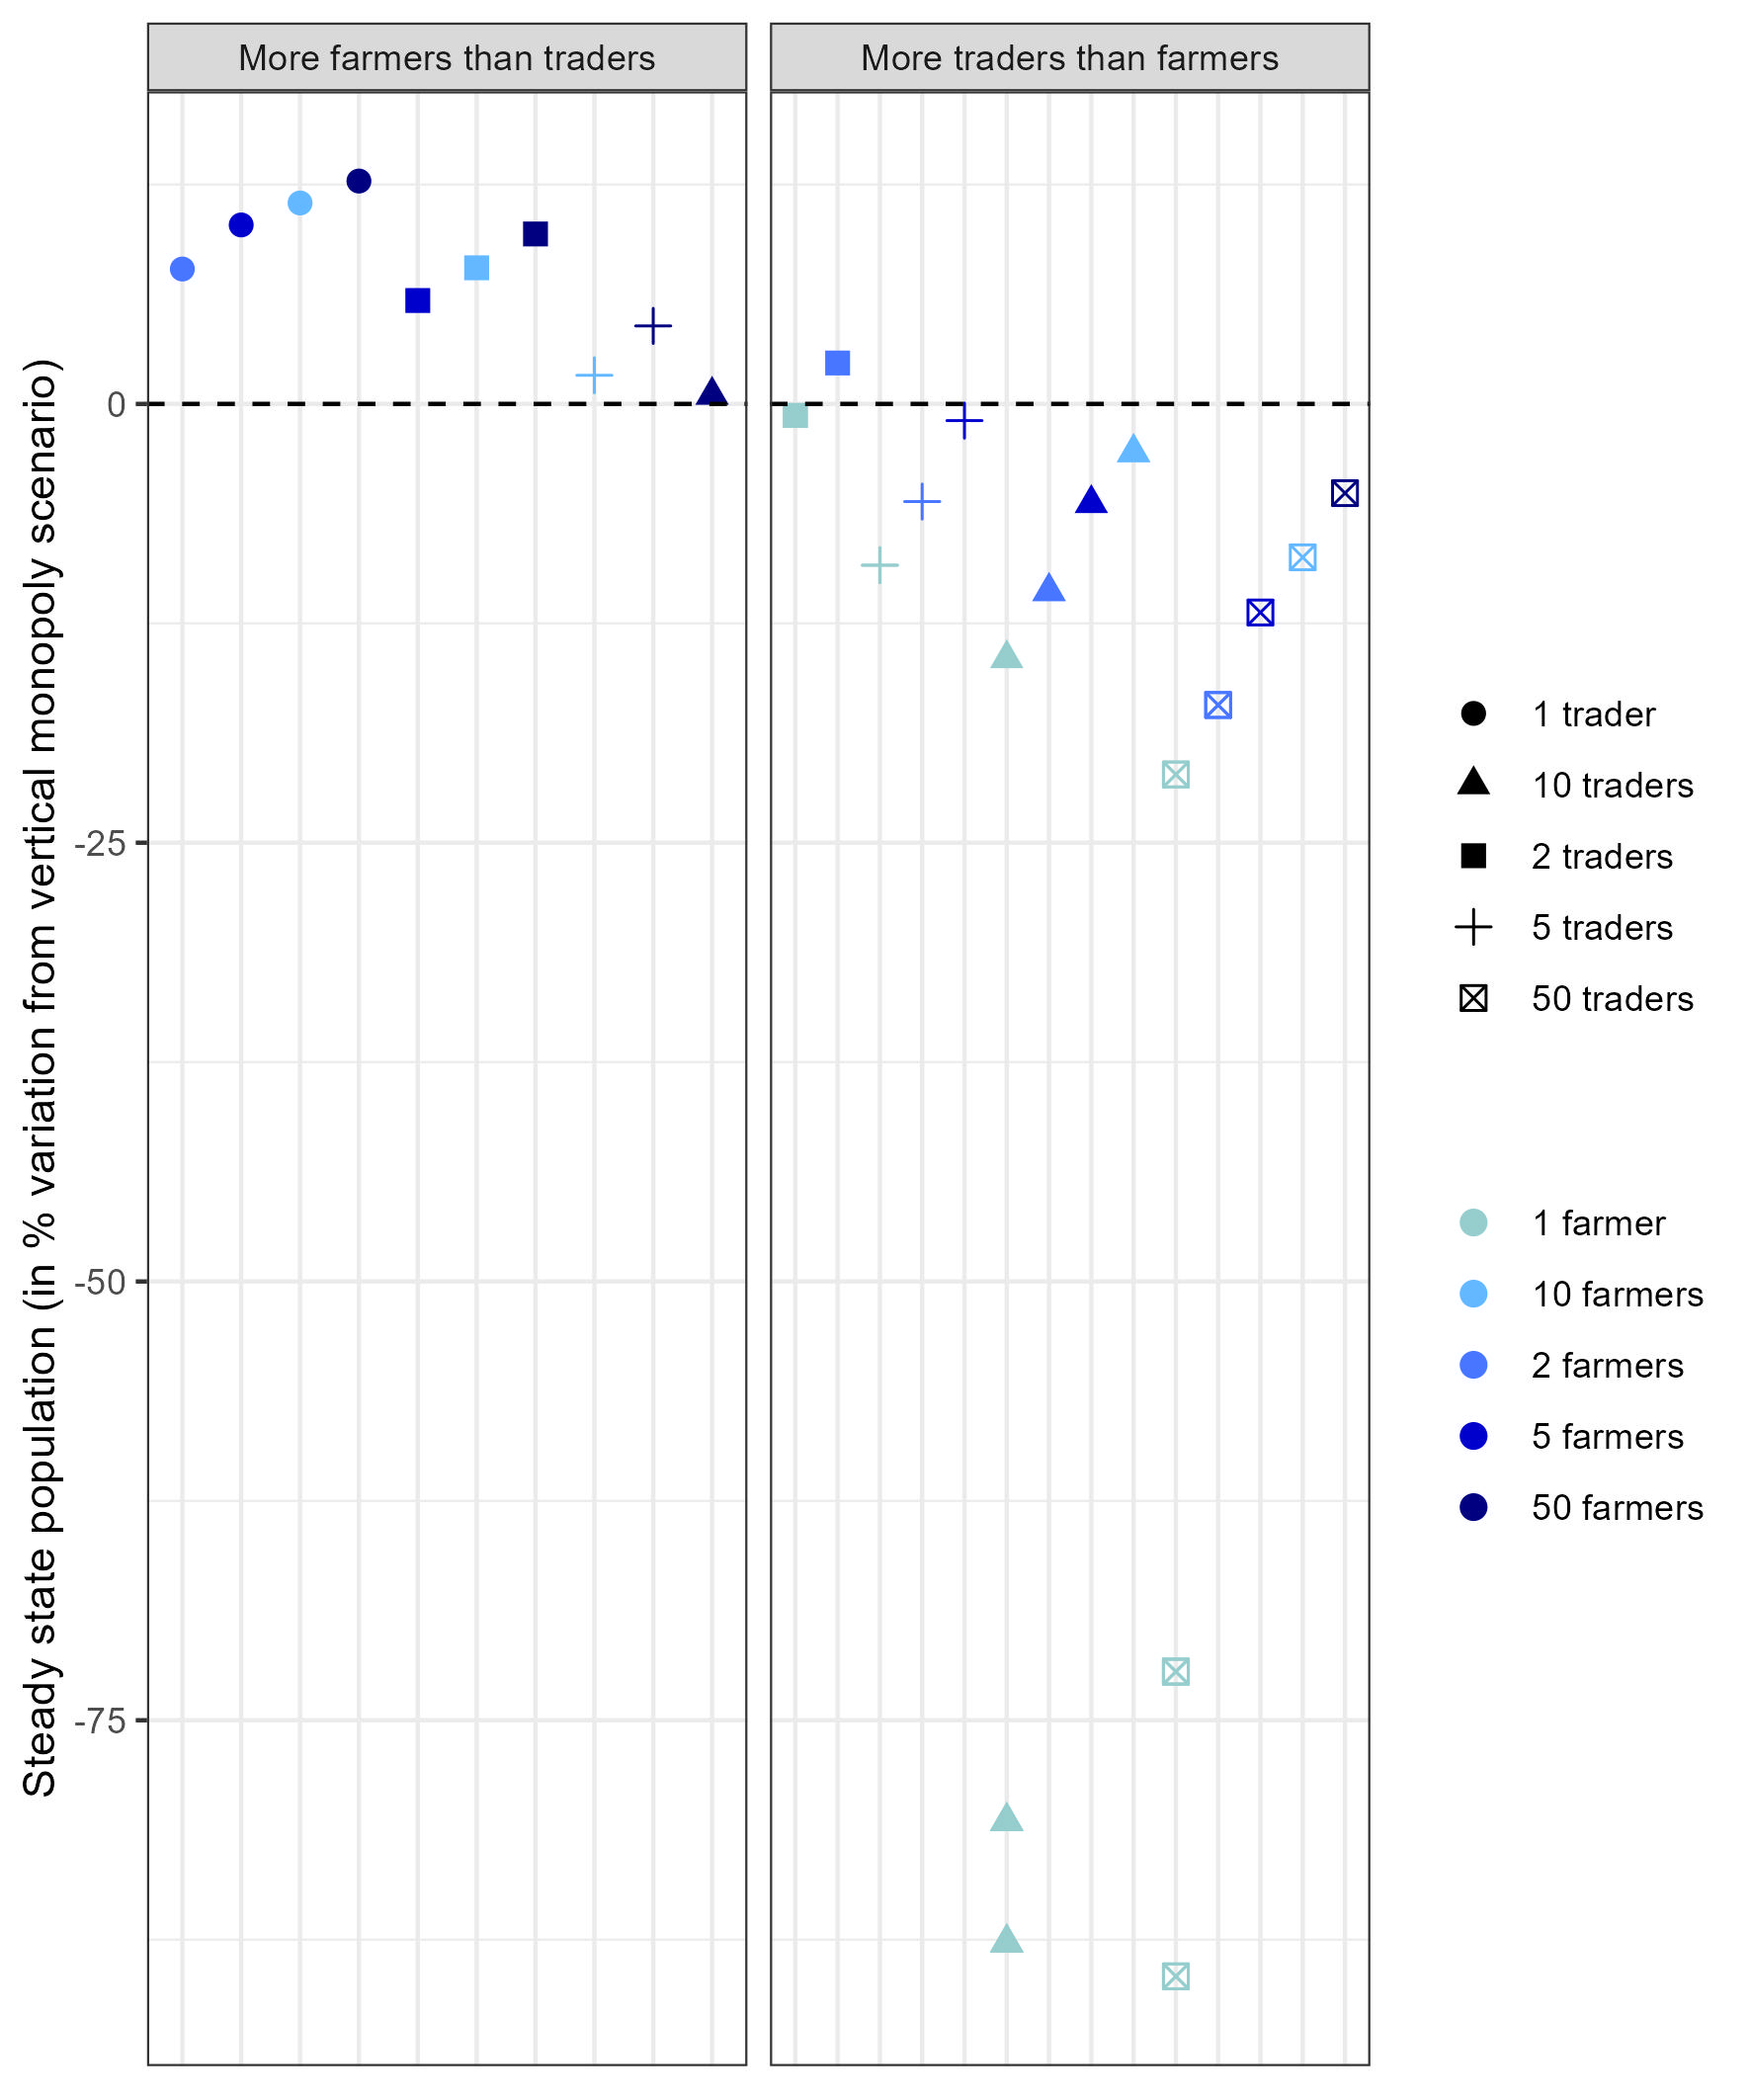
\includegraphics[width=.7\textwidth]{figures/totoaba/sup_figure1.jpg}
    \caption{Steady state outcomes when multiple traders and multiple farmers are  considered (an oligopoly) in the quantity adjustment scenario.}
    \subcaption*{ The left panel shows the steady state of the wild \textit{Totoaba macdonaldi} population when there are more farmers than traders. The right panel shows the steady state of the wild population when there are more traders than farmers}
    \label{fig:cournot_oligo}
\end{figure}
%
\paragraph{Bertrand oligopoly}
Using the same notations as previously, the demand functions can be written as : 
\begin{align}
    \forall i\in \mathcal{I} : q^W_i = q^W = \frac{1}{N}(a^W - b^W P^W - e P^F)\\
    \forall j \in \mathcal{J} : q^F_j = q^F = \frac{1}{M}(a^F - b^F P^F - e P^W)
\end{align}
Using these demand functions and solving for the reaction functions in each case yields : 
\begin{align}
    r^F(P^W) &= \frac{a^F + b^F v + eP^W}{2b^F}\\
    r^W(P^F) &= \frac{a^W + b^W (s+c) + e P^F}{2b^W}
\end{align}
These reaction functions are the same as in the duopoly case (see eq. \ref{eq:rf_bertrand}). This result shows that aggregate production is invariant to the number of farmers or traders as long as both are present on the market. Moreover, the individual production for traders is $\frac{1}{N} q^W_B$ and $\frac{1}{M}q^F_B$ with $q^W_B$ and $q^F_B$ referring to the duopoly equilibrium quantities for poached and farmed productions. In a Bertrand equilibrium, irrespective of the number of players, price-setting competition pushes the price to its minimum such that both firms still operate (given that traders have a stock-dependent production cost). Increased competition in the form of more players cannot push the prices further down. Therefore, aggregate output remains the same and individual production is divided among players. \\
This result further contradicts the results in \cite{damania_economics_2007}, as the authors find that increasing the number of players in a Bertrand set-up has detrimental effects on the steady-state stock. We find no effect, consistent with the theory and intuition. 
%
\subsubsection{Trader take over of the aquaculture sector}
%
In this section, we look at the 'extended cartel' scenario, where the vertical monopoly takes over the ownership of the aquaculture firm. \\
To gain intuition, assume poached and farmed products are perfect substitutes. On the one hand, the vertical monopoly has two production technologies:  poaching ( with a variable marginal cost, as the price paid to poachers depends on the population stock) and farming ( with a constant marginal cost). In this case, the vertical monopoly equates the marginal costs across production units; that is, it buys a poached product to poachers up until the marginal cost of an extra poached unit equates to that of a farmed unit. In this case, if the marginal cost of farming is lower than market prices absent farming, then poaching goes down. Notice that the only way for traders to limit the price paid to poachers is to maintain a healthy stock. Therefore, the new equilibrium population stock is larger than the initial stock, and poaching is lower.

Now consider the case at stake, where products are imperfect substitutes. In this case, the extended cartel does not only equate marginal costs, as marginal revenues diverge across products. We use the following model to investigate the resulting equilibrium. Let the profit of the extended cartel be:

\begin{equation}
\Pi(q^F, q^W) = (\alpha^W - \beta^W q^W - \gamma q^F - (s+c))q^W + (\alpha^F - \beta^F q^F - \gamma q^W - v)q^F
\end{equation}

The extended cartel maximizes its profit with respect to the poached and farmed products. The poached production it sells on end markets is : 

\begin{equation}
q^W = \frac{\sigma^2 x^2 (\beta^F(\alpha^W -c) - \gamma (\alpha^F - v)) - W_1 \beta^F \sigma x }{2(\beta^F W + \sigma^2 x^2 (\beta^F \beta^W - \gamma^2)) }
\end{equation}

Figure \ref{fig:extended_cartel} shows that if the 'extended cartel' scenario arises, poaching goes down, and the steady-state population increases.
%
\begin{figure}
    \centering
    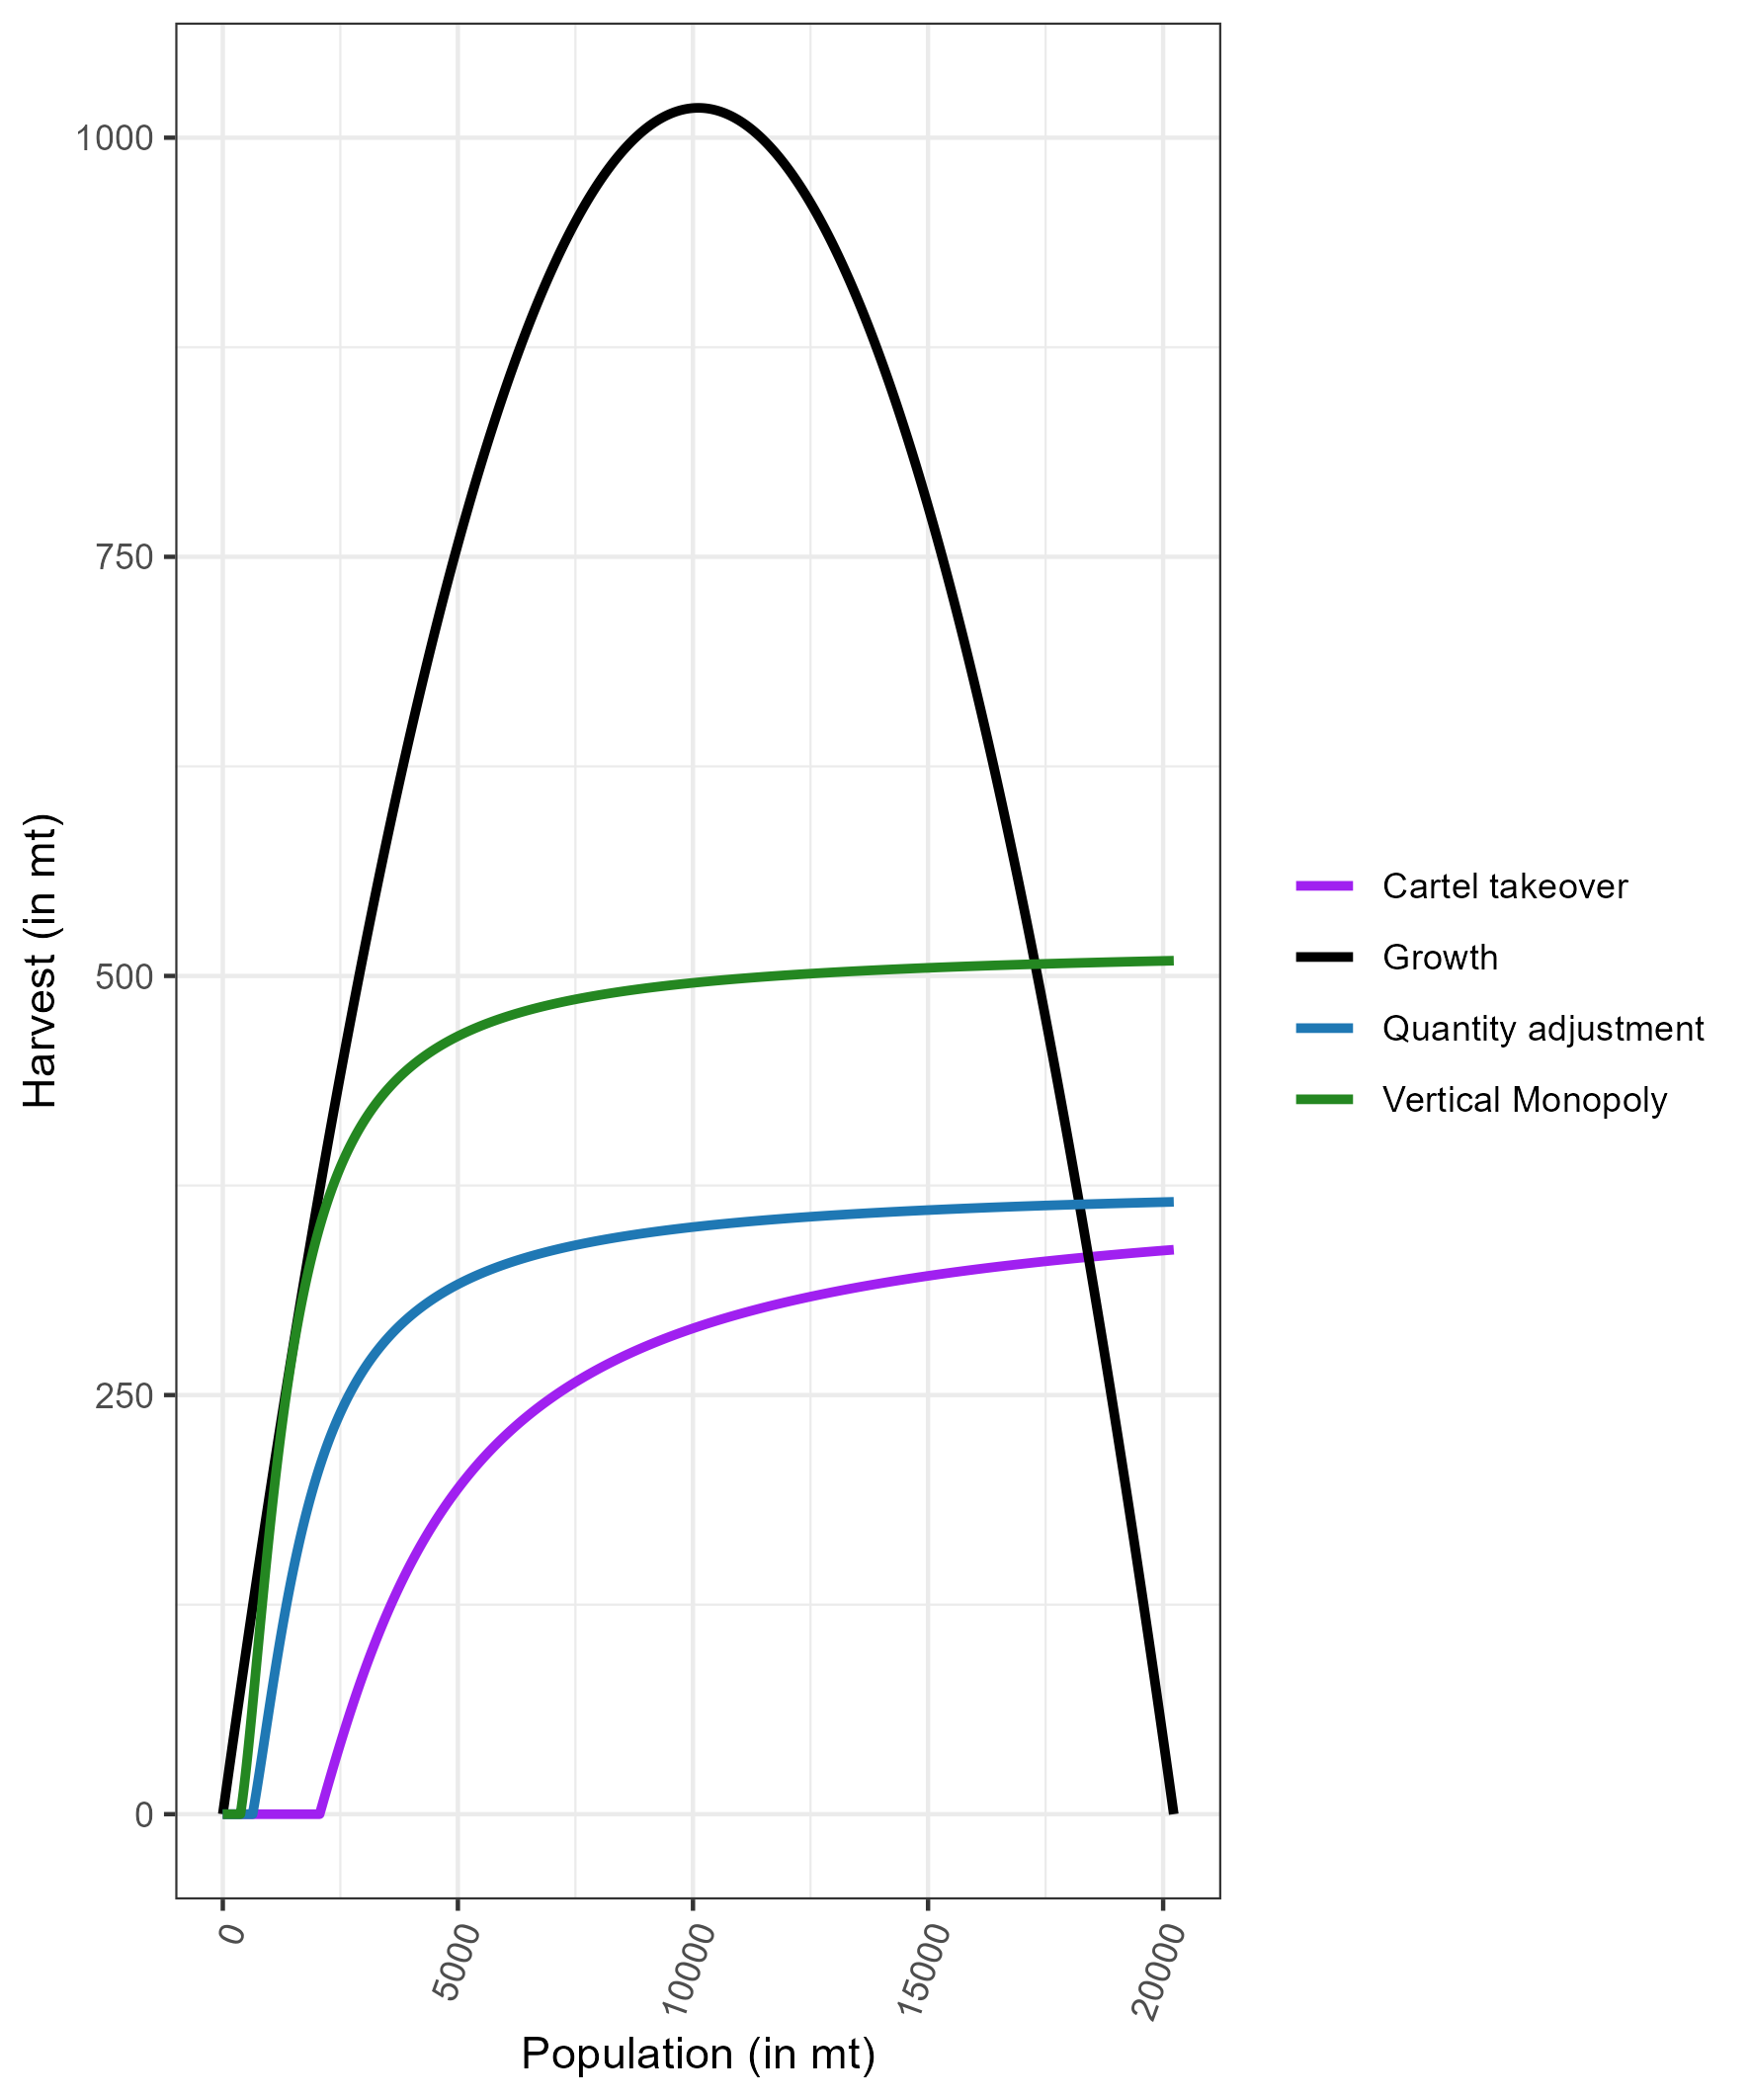
\includegraphics[width = .7\textwidth]{figures/totoaba/sup_figure2.png}
    \caption{ Steady-state equilibrium for the wild stock of \textit{Totoaba macdonaldi }in the ‘extended cartel’ scenario, where the vertical monopoly takes over the ownership of farming operations}
    \label{fig:extended_cartel}
\end{figure}

\subsection{Appendices}
\label{subsection:appendix_toto}
\subsubsection{Lemma 1 : content and proof}
\label{section:AppendixB}

Assume $\alpha^W = \alpha^m$ and $\beta^m  =\beta^W$, i.e., that the demand faced by the monopolist is the same as in the duopolistic case.  Comparing monopoly and Cournot harvest functions:
\begin{align*}
q^W_m &\geq q^W_c\\
    \Rightarrow v & \leq \Bar{v}=\alpha^F - \frac{\gamma(\alpha^m - c)\sigma^2x^2 - W_1\sigma x}{2\beta^m\sigma^2x^2 + 2W}
\end{align*}
First, look at when $x \to 0$ : 
$$
\lim_{x\to 0}\Bar{v} = \alpha^F
$$
This requires that farming costs are lower than the choke price for consumers on their market. This condition is necessary for a farm competitor to enter the market. 
\\
Second, acknowledge that the second part of the equation is weakly decreasing, but non-increasing. Assuming the carrying capacity goes to infinity, it is limited by :
$$
\lim_{x \to \infty}\Bar{v} = \alpha^F - \gamma\frac{(\alpha^m - c)}{2\beta^m}
$$
As fish abundance increases, the price paid to poachers decreases, as there is less scarcity. From equation (\ref{eq:price_poachers_cournot}), when $x \to \infty$, the price paid to poachers drops to 0. 
Moreover, notice that the last term in parenthesis is equation (\ref{eq:monop}) for $s=0$. Therefore, it means that the residual willingness to pay, when the poachers behave like a monopoly and $x\to \infty$, is larger than the unit cost of farming. 

If the market is truly duopolistic, in the sense that the poachers could not manage the stock such that they depress demand so much as to kick their competitor out of the market, then Cournot competition unambiguously leads to lower poaching levels than a monopoly does.
%
\subsubsection{Lemma 2}
\label{section:AppendixC}
Assume that the demand parameters are unchanged by the introduction of farmed substitutes, that is to say $\alpha^W  = \alpha ^m$ and $\beta^W= \beta^m$, and use the definition of the coefficients for the direct demand function:
\begin{align*}
 a^{j} &= \frac{\alpha^{j} \beta^{i} - \alpha^{i}\gamma}{\beta^{j} \beta^{i} - \gamma^2}; \hspace*{1cm}
  b^{j} = \frac{\beta^{i}}{\beta^{j} \beta^{i} - \gamma^2}\\
 a^m &= \frac{\alpha^m}{\beta^m}; \hspace*{2cm}
b^m = \frac{1}{\beta^m}
\end{align*}
For $i,j \in \{W, F\}$ and $m$ the monopoly case.
To establish Lemma 2, we compare $q^W_B$ and $q^W_m$. Equation (\ref{eq:harvest_monop}) can be rewritten as : 
$$
q^m(a^m, b^m) = \frac{\sigma^2 x^2(a^m - b^m c) - b^m W_1 \sigma x}{2\sigma^2 x^2 +2Wb^W}
$$
%
Therefore:
\begin{align*}
    &q^W_m \geq q_B^W\\
    \Rightarrow & v \leq \frac{a^m - b^m c}{b^Wb^Fe}\left[ \frac{2 W_2 b^W(2b^Fb^W - e^2) + (4b^Fb^W - e^2)\sigma^2 x^2}{2 \sigma^2 x^2 + 2 b^m W_2}\right]  - \frac{W_1 \sigma x[(4 b^F b^W - e^2)(b^m - b^W) + e^2 b^W]}{b^wb^Fe(2\sigma^2 x^2 + 2b^m W_2)} \\
    & - \frac{ea^F + c(e^2 - 2b^Wb^F) + 2b^F a^W}{b^F e}
\end{align*}
Notice that this equation can be reframed as : 
\begin{align*}
    F(x|c) \geq v \text{ where } F(x|c) = \Phi \frac{\eta + \mu x^2}{\theta + \nu x^2} -\frac{ \kappa x}{\omega x^2 + \epsilon} - \zeta
\end{align*}
And :
\begin{align*}
    &\Phi = \frac{a^m - b^mc}{b^W b^F e},\text{ }
    \eta = 2W_2b^W(2b^Wb^F - e^2),\text{ } 
    \mu = (4b^Wb^F - e^2)\sigma^2,\text{ }\\
    &\theta= 2W_2b^m,\text{ }
    \nu = 2\sigma^2,\text{ }
    \zeta  = (ea^F + c(e^2 - 2b^W b^F) + 2b^F a^W)\\
    \\
    &\kappa = W_1 \sigma [(4b^F b^W - e^2)(b^m - b^W) + e^2 b^W)], \\
    &\text{ }\omega = 2b^Wb^Fe \sigma^2
    \text{ and } \epsilon = 2b^m b^W b^F e W_2
\end{align*}
\paragraph{Analysis of $\Phi \frac{\eta + \mu x^2}{\theta + \nu x^2}$:} if $\mu \theta - \nu \eta<0$, the first component of $F(x|c)$ is decreasing:
\begin{align*}
&(4b^Wb^F - e^2)b^m -2(b^Wb^F-e^2)b^W<0\\
\iff & \frac{\gamma^2}{\beta^m (\beta^W\beta^F - \gamma^2)^3}\left[ \beta^m \beta^F + \gamma^2 -4\beta^F \beta^W \right]<0\\
\end{align*}
Under the assumption that $\beta^m = \beta^W = \beta^F = \beta$, it is clear that 
$$
\frac{\gamma^2}{\beta(\beta^2 - \gamma^2)}(\gamma^2 - 3 \beta^2) <0
$$
as $\gamma < \beta$. 
\paragraph{Analysis of $\frac{\kappa x}{\omega x^2 + \epsilon}$}: the second component of $F(x|c)$ is increasing for $x \leq \sqrt{\frac{\epsilon}{\omega}}$, and decreasing after, since $x\in \mathbb{R}^+$. Noticing that $\kappa <0$: 
\begin{itemize}
    \item For $x \in \left[0,\frac{1}{\sigma}\sqrt{W_2 b^m} \right]$, $\frac{\kappa x}{\omega x^2 + \epsilon}$ is decreasing
    \item For $x>\frac{1}{\sigma}\sqrt{W_2 b^m}$ is increasing
\end{itemize}

\paragraph{Conclusion}
Overall, $F(x|c)$ is such that : 
\begin{itemize}
    \item For $x \leq \frac{1}{\sigma}\sqrt{W_2 b^m}$, the first component is decreasing, while the second component is increasing
    \item For $x \geq \frac{1}{\sigma}\sqrt{W_2 b^m}$, the first component is decreasing and the second component is decreasing
\end{itemize}

Hence, $F(x|c)$ is bounded above by $\max \big(F(0|c),F(\frac{1}{\sigma}\sqrt{W_2 b^m}|c)\big)$, and bounded below by $F(K|c)$ where $K$ is the system carrying capacity. Therefore:
\begin{enumerate}
    \item If $v<F(K|c)$, then Bertrand harvest is always lower than monopoly harvest
    \item If $F(K|c)<v<F(0|c)$, then Bertrand harvest starts by being lower than in the monopoly case, but gets larger for large stock values. 
    \item Eventually, if $F(0|c)<v$, then Bertrand harvest is always larger than in the monopoly case
\end{enumerate}
%Figure \ref{fig:bertrand_proof} illustrates this property. The top, red, dashed curve corresponds to case 1, where Bertrand always yields a larger harvest. For intermediary values, first, in the red-shaded area, Bertrand harvest is lower than in the monopoly case. For large stock values, however, it becomes larger than in the monopoly case, as displayed in the black-shaded area. Eventually, the bottom, black, dotted curve shows low values of $v$ where Bertrand harvest is always lower than in the monopoly case.

%\begin{figure}[H]
%    \centering
%    \includegraphics[width = .6\textwidth]{figures/Figure6_Lemma4_zoomed.jpg}
%    \caption{$F(x)$ and $v$ summarise when Bertrand harvest is larger or lower than in monopoly. In the red-shaded area, Bertrand harvest is lower than in the monopoly case. In the grey-shaded area, it is larger. }
%    \label{fig:bertrand_proof}
%\end{figure}

\paragraph{Corner equilibrium:}
for a corner solution to emerge, it must be that $q_B^{w*}=0$,
\begin{equation}
    v = v(x) = \frac{W_1(2b^F b^W - e^2)}{\sigma x b^F e} - \frac{2b^F a^W + ea^F + c(e^2 - 2b^W b^F)}{b^F e }
    \label{eq:v_corner}
\end{equation}
Equation \ref{eq:v_corner} shows that for low stock values, costs can still be positive and poaching disappear. However, to ensure that poaching is \textit{never} beneficial in the Bertrand equilibrium, it must be that $v = \min v(x) = - \frac{2b^F a^W + ea^F + c(e^2 - 2b^W b^F)}{b^F e v}$. In this case, the subsidy rate is so high that production is always beneficial for the farmer, and prices are too low for the trader to compete. In our baseline specification, this would amount to $v = - 720,855$ USD.  

%Figure \ref{fig:v_poaching_stop} shows the evolution of $v$ as substitutability and trading costs vary. 
%\begin{figure}[H]
%    \centering
%    \includegraphics[width = .8\textwidth]{figures/Figure7_v_poaching_stop.jpg}
%    \caption{$v$ for poaching to stop in a Bertrand equilibrium as a function of $\gamma$ and $c$}
%    \label{fig:v_poaching_stop}
%\end{figure}
%\subsubsection{Linear quadratic cost model}
%\label{sec:linear quadratic}

%In this section, we use a different cost specification for the fishery : 
%\begin{equation}
%    C(E) = W_1 E + W_2 \frac{E^2}{2}
%\end{equation}

%In this case, optimal effort is : 
%\begin{equation}
%    E^* = \frac{s\sigma x - W_1}{2W_2}
%\end{equation}
%And the quantity provided is : 
%\begin{equation}
%    q^W = \frac{s\sigma^2 x^2 - W_1 \sigma x}{2W_2} 
%\end{equation}

%\paragraph{In the vertical monopoly equilibrium,} demand from the monopoly does not change, but the supply does. 

%\begin{align}
%    \text{Price paid to poachers :} s^*_m(x) &= \frac{W_2 (\alpha_m -c) + \beta^m (W_1 \sigma x) }{ \sigma^2 x^2 \beta^m + W_2 }\\
%        \text{Poaching : } q^*_m(x) &=\frac{\sigma^2 x^2 (\alpha_m - c) - W_1 \sigma x}{2(\sigma^2 x^2 \beta^m +W_2)}
%\end{align}


%\paragraph{In the Cournot equilibrium, } demand remains unchanged, but supply is changed. 
%\begin{align}
%    \text{Price paid to poachers: } s_C^*(x) &= \frac{2 W_2(2\beta^F(\alpha_w - c) - \gamma(\alpha^m - v)) + W_1 \sigma x(4\beta^F\beta^W - \gamma^2)}{4W_2 \beta^F + \sigma^2 x^2(4\beta^F\beta^W -\gamma^2)} \\
%    \text{Poaching : } q^{C*}_W(x) &= \frac{\sigma^2 x^2(2\beta^F(\alpha^w -c) - \gamma(\alpha^F - v)) - 2\beta^F W_1 \sigma x}{4 W_2 \beta^F + \sigma^2 x^2(4\beta^W \beta^F - \gamma^2)}
%\end{align}

%\paragraph{In the Bertrand equilibrium }
%\begin{align}
%    \text{Price paid to poachers : } s_B^*(x) &=\frac{2 W_2 b^W[b^F(2a^w + ev) + e a_F + c(e^2 - 2b^Wb^F)] + W_1 \sigma x (4b^Fb^W - e^2)}{\sigma^2 x^2 (4b^F b^W - e^2) + 2 W_2 b^W(2b^F b^W - e^2)}
%\end{align}

%We use data collected at the vessel level to calibrate $W$ in the main specification and calibrate the marginal cost of effort to be equal to the observed average cost (the residual being a fixed cost parameter) in our data.

%Given that we have a 2 unknown equations for a single solution, a wide range of solutions for $W_1$ and $W_2$. Figure \ref{fig:equilibria_lq} shows the equilibria emerging from different $W_1$ and $W_2$ values. For specifications where the quadratic parameter $W_2$ is low, the \textit{vertical monopoly} can result in a drastic decline in steady-state population, while introducing aquaculture still yields substantial benefits in terms of steady-state population. For intermediate weights between the linear and quadratic parameters, results do not change drastically, and for large values of the quadratic parameter, results are not significantly different. Note that under the linear quadratic specification, low steady-state populations do not emerge in the price setting (Bertrand) equilibrium. 



\newpage
%\section{Supplementary data and empirical results}
%\subsection{Data}
%\subsubsection{Parameters for calibration}
%See table \ref{tab:params}.


%\subsubsection{Information about the cost of poaching}

%See table \ref{tab:costW}


%\subsubsection{Information about the cost of farming}
%See table \ref{tab:costv}


%\subsubsection{Demand estimation}
%See table \ref{tab:demand}


%\subsubsection{Individual growth curves for farmed versus wild totoaba, using the von Bertlaffery growth}
%See figure \ref{fig:vbgf}

%\subsection{Empirical results}

%\subsubsection{Impact of aquaculture on steady-state stock in different market structures}
%See table \ref{tab:oa_comp_aquaculture}

%\subsubsection{Impact of farming and transaction costs on equilibria}
%See figure \ref{fig:cost_equilibrium}.




%\subsubsection{Impact of demand variation and substitutability on steady state populations}
%Figure 4 (in manuscript) shows the evolution of steady-state populations in the market structures under study. The three different panels show results for values of $\gamma$ such that $\gamma \in \{ 0.1\beta, 0.5\beta, 0.9\beta \}$. 

%The three quadrants, delineated by dotted lines, display the type of equilibrium: the top panel is the high, stable state, the middle panel is the middle, unstable state, and the bottom panel is the low and stable state. Results show that the interaction between the expansion of demand and the substitutability of goods creates nontrivial results.

%First, in the monopoly case, increasing demand unambiguously leads to (i) the apparition of low, stable steady states (when $\alpha' >1.2 \alpha)$ and (ii) lower steady-state values. When farming is introduced, if demand increases, the effect of substitutability is key. 

%For low substitutability values,  competition increases the steady state values, compared to monopoly if it were to face increased demand.
%However, they yield significantly lower values than in the status quo equilibrium. When substitutability increases, and low stable steady states emerge. When substitutability increases ($\gamma = .5\beta$), Cournot competition can accomodate a 20\% increase in demand without harming the stock. If Bertrand equilibrium were to arise, it would result in a lower steady state equilibrium than the status quo equilibrium. The threat of low stable steady states emerges as well. When substitutability between products is large ($\gamma = .9\beta$), a Cournot outcome can accomodate a 40\% increase in demand, while population in a Bertrand equilibrium would be severely depleted. 

%Overall, substitutability has bifurcation values, changing the nature of the equilibria (1 equilibrium \textit{v.} 3 equilibria) as demand increases. When substitutability is large enough, demand can increase without changing the structure of the equilibria. 
%\newpage

%\section{Supplementary discussion and conclusion}


%Several assumptions underlie our results.

%First, we implicitly assume that the vertical monopoly does not discount future profits. Notwithstanding this polar assumption, economic theory shows that if profits are linear in effort, a monopolist owner of a renewable resource will lead to less effort, less catch and a larger population at a steady state, with a positive discount rate \citep{Crutchfield1962}

%Our set-up uses a fisher profit function that is quadratic in effort, and no discounting from the vertical monopoly. Simulations yield similar results. It is unclear how a positive discount rate would impact our conclusions (both in terms of existence and stability of the equilibrium) but our conclusions are robust to varying parameters that impact the ptimal response in a similar way.

%Second, we assume that farming rotations are invariant to market structure (following \cite{MITRA1986229}). However, existing results may be challenged as the model may be seen as artificially restrictive. In this case, they assume full replacement of the resource (i.e, when one fish is harvested, a new one has to spawn), as well as fixed production capacity (in their case, fixed land for forestry), and the life-span of a resource (i.e, they do not allow for a resource to go beyond a certain age). In doing so, they do not allow for adjusting production capacity nor how and when production reached the market. Further research is needed to actualize this result. 

%Third, we assume a linear demand model where quality does not play a role. In real life, there is a size/age premium for totoaba swim bladders. Our model takes the average quality as given. As the distribution of swim bladder size seems skewed to the left, aquaculture could operate on a luxury market and further displace demand. 


%Third, we assume that the cost structure of farming is linear, and does not depend on the wild population stock. However, as stocks plummet, security expenses are likely to increase\footnote{Famous examples include farming of rhinos, where security expenses skyrocketed as the rarity of rhino horns increased (see \url{https://www.cbsnews.com/news/rhino-farm-auction-john-hume-seeks-billionaire-to-carry-on-conservation-work/ })}. Therefore, costs may be quadratic in the stock. Eventually, the ecological requirement for farming and the corresponding location of the farming operation are important variables in limiting security expenses.
\newpage

\section{Supplementary Figures and Tables}
\begin{figure}[H]
    \centering
    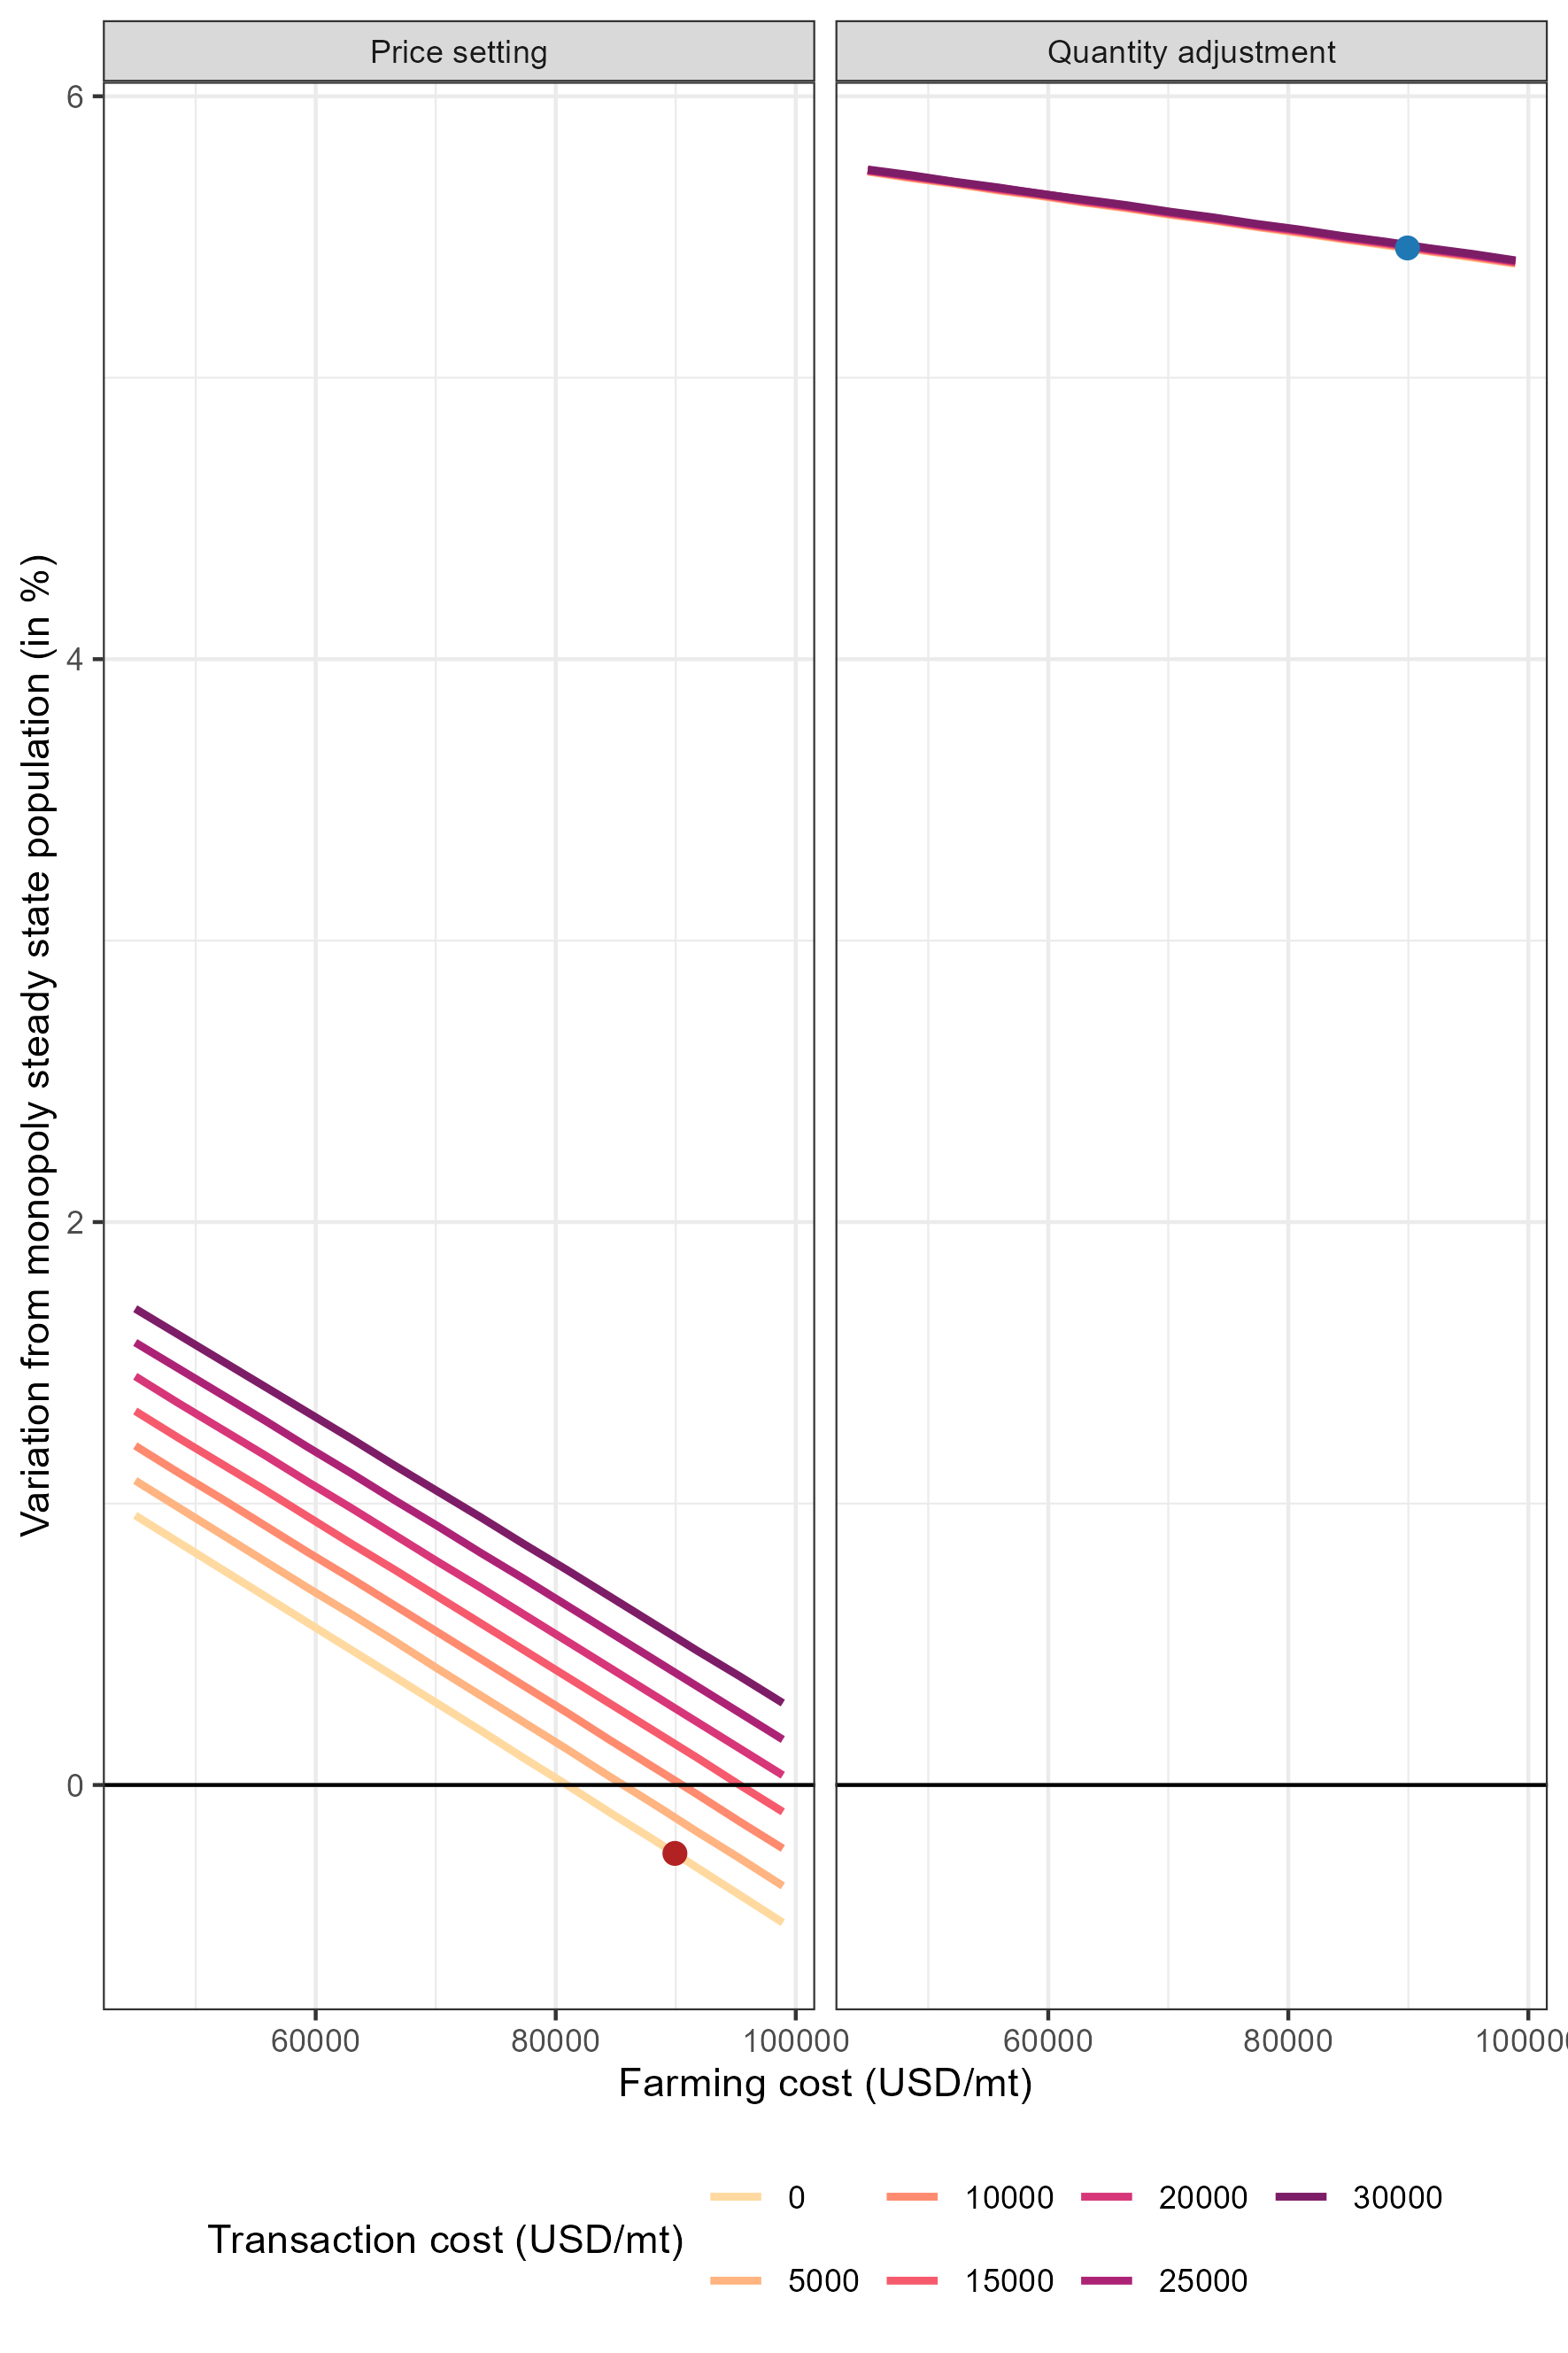
\includegraphics[width = .7\textwidth]{figures/totoaba/sup_figure3.png}
    \caption{Percent change in steady state population across scenarios, following the joint evolution of illegal transaction and farming costs}
    \subcaption*{Red and blue dots represent baseline results in the price setting and quantity adjustment scenarios}
    \label{fig:c_and_v}
\end{figure}
\newpage

%\setcounter{figure}{3}    

\begin{figure}[H]
    \centering
    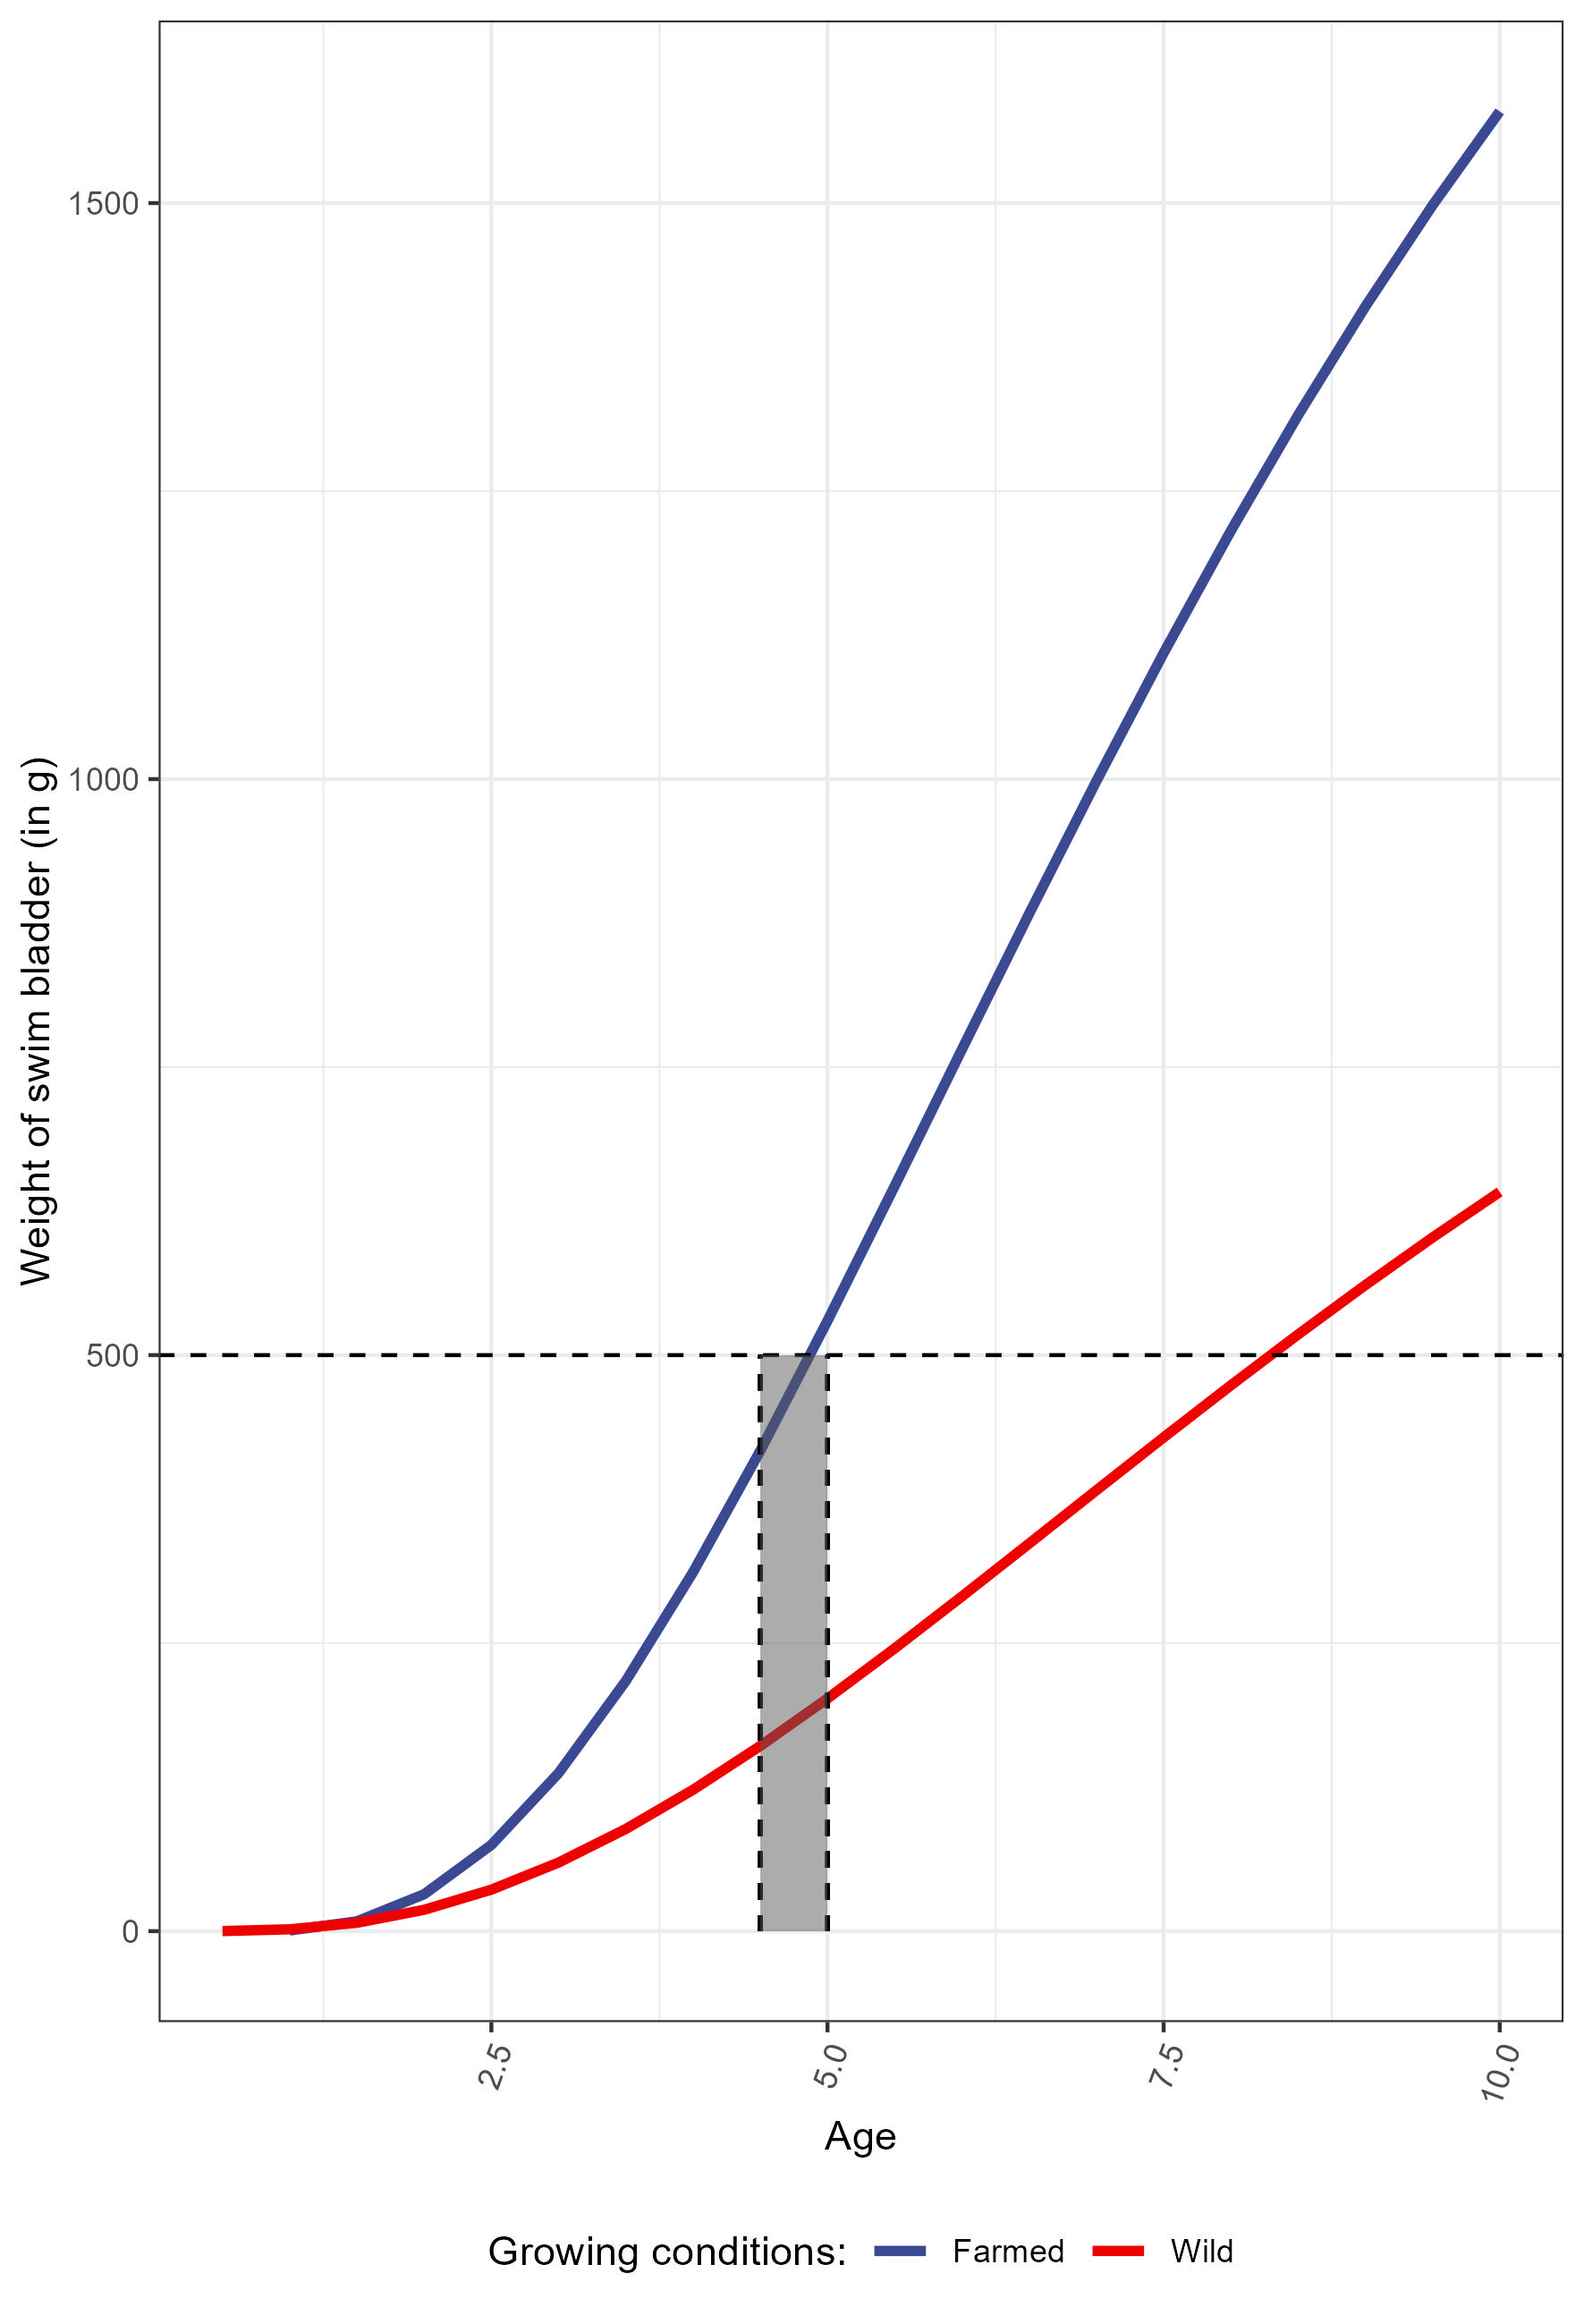
\includegraphics[width = .7\textwidth]{figures/totoaba/sup_fig4_VBGF_growth.jpg}
    \caption{Von Bertalanffy Growth curves for wild and farmed \textit{Totoaba macdonaldi} under different growing conditions}
    \subcaption*{
    Gray box indicates the range of ages that possess a 500 gram swim bladder. The wild individual growth curve was calibrated with information from the stock assessment, while the farmed individual growth curve was calibrated using}
    \label{fig:vbgf}
\end{figure}


\newpage

\begin{landscape}
\begin{table}[H]
%\caption{}
\centering
\begin{tabular}[t]{ccccc}
\hline 
Variable & Low Season & Mid Season & High Season & Source\\
\hline \hline
Vessels & 5 & 20 & 50 & \cite{cisneros-mata_evaluacion_2020} \\
Days per month & 4 & 12 & 14 & \cite{cisneros-mata_evaluacion_2020}\\
Total fleet days year & 20 & 240 & 700 & \cite{cisneros-mata_evaluacion_2020}\\
Food fuel day & 525 & 525 & 525 & Semi-Structured Interviews\\
Totoaba gearset & 2 & 3 & 6 & \cite{cisneros-mata_evaluacion_2020}\\
Gear loss day & 0.5 & 0.5 & 0.5 & Semi-Structured Interviews\\
Gearset vessel per day & 2 & 3 & 3 & \cite{cisneros-mata_evaluacion_2020}\\
Gear replacement & 1600 & 1600 & 1600 & Semi-Structured Interviews\\
Bribes/year & 600 & 7200 & 21000 & Semi-Structured Interviews\\
\hline 
Average cost (per vessel day) & 8385.34 & 14386.69 & 5051.26 & Authors' calculation\\
\hline \hline
\end{tabular}
\label{tab:costW}
\caption{Supporting information for the calculation of the\textit{ Totoaba macdonaldi} poaching cost parameters ($W_1$ and $W_2$). The methods section details how and when semi-structured
 interviews were conducted.}
\end{table}
\end{landscape}
\newpage

\begin{landscape}
\begin{table}[H] 
\centering 
%  \caption{} 
  \label{} 
\begin{tabular}{@{\extracolsep{5pt}}lc} 
\\[-1.8ex]\hline 
\hline \\[-1.8ex] 
 & \multicolumn{1}{c}{\textit{Dependent variable:}} \\ 
\cline{2-2} 
\\[-1.8ex] & Price \\ 
\hline \\[-1.8ex] 
 Catch & $-$1,563.752$^{**}$ \\ 
  & (725.985) \\ 
  & \\ 
 Constant & 1,625,837.000$^{***}$ \\ 
  & (406,789.500) \\ 
  & \\ 
\hline \\[-1.8ex] 
Observations & 45 \\ 
R$^{2}$ & 0.097 \\ 
Adjusted R$^{2}$ & 0.076 \\ 
Residual Std. Error & 431,737.700 (df = 43) \\ 
F Statistic & 4.640$^{**}$ (df = 1; 43) \\ 
\hline 
\hline \\[-1.8ex] 
\textit{Note:}  & \multicolumn{1}{r}{$^{*}$p$<$0.1; $^{**}$p$<$0.05; $^{***}$p$<$0.01} \\ 
\end{tabular} 
\label{tab:demand}
\caption{Regression output for the linear demand estimation calculated by regressing price data on catch data. }
\subcaption*{Data were obtained from the available literature that provided estimated weight and value
 of \textit{Totoaba macdonaldi} maw seizures on estimated \textit{Totoaba macdonaldi} catch from 2014 to 2017
 obtained from a recent stock assessment. The methods section details where information was obtained from. }
\end{table} 
\end{landscape}
\newpage

\begin{landscape}
\begin{table}[H]

\centering
\begin{tabular}[t]{ccc}
\hline
Variable & Value & Source\\
\hline\hline
Sphere & 1.00 & Earth Ocean Farm Video, 2022\\
Capacity per sphere (t) & 144.00 & Earth Ocean Farm Video, 2022\\
\hline \hline
\textit{In \$USD} & & \\
\hline
Maintenance year & 12500.00 & Felipe Ramirez, InnovaSea, 2018\\
Cleaning year & 5000.00 & Felipe Ramirez, InnovaSea, 2018\\
Vessel maintenance/year & 10000.00 & Tyler Korte, BlueOcean Mariculture, 2018;\\
& & 
Fernando Cavalin, Earth Ocean Farms, 2018\\
Fuel year & 25122.50 & Author's Calculations\\
Feed & 312480.00 & Tyler Korte, BlueOcean Mariculture, 2018\\
Labor & 1580000.00 & Authors' calculations\\
Facility lease & 150000.00 & Cygnus Ocean Farms, 2017\\
Admin. & 50000.00 & Cygnus Ocean Farms, 2017\\
\hline
Operational costs & 2145102.50 & Authors' calculations\\
Operational costs (per t \& year) & 14896.55 & Authors' calculations \\
\hline
\end{tabular}
\caption{Supporting information for the calculation of the \textit{Totoaba macdonaldi} farming cost parameter ($v$)}

\subcaption*{Annual cost estimates were obtained from informants and converted to \$USD. Capacity of each farming pen was obtained from Earth Ocean Farms, and an annual cost
706 per tonne of totoaba was calibrated using personal communications with totoaba aquaculture producers.}
\label{tab:costv}
\end{table}
\end{landscape}

\newpage



%\begin{table}[H]
%\centering
%\begin{tabular}[t]{cccc}
%\hline
%Parameter & Value & Concept & Units\\
%\hline \hline
%$\alpha$ & 1625836.98 & Demand model : intercept & USD\\

%$\beta$ & 1563.75 & Demand model : coefficient & USD/metric ton of biomass\\

%$r$ & 0.20 & Intrinsic growth rate & unitless\\

%$K$ & 20226.00 & Carrying capacity (in metric tons)   & \% of biomass/vessel trip\\

%$\sigma$ & $2\times 10^{-5}$ & Catchability & metric tons of biomass\\

%$Avg cost $& 8385.34 & Average cost per vessel trip & USD\\

%$W_{mid}$ & 2.18 & Parameter cost ($MC = Avg$) at historical value - middle & USD\\

%$W_{low}$ & 1.32 & Parameter cost ($MC = Avg$) at historical value - low & USD\\

%$W_{high}$ & 3.75 & Parameter cost ($MC = Avg$) at historical value - high & USD\\

%$Age$ & 4.50 & Age of farmed totoaba & Years\\

%$\gamma$ & 1407.38 & Substitutability & Unitless\\

%$v$ & 67034.45 & Unit cost of farming & USD/metric ton of biomass\\

%$c$ & 0.00 & Unit cost of trading & USD/ metric ton of biomass\\
%\hline
%\end{tabular}
%\caption{Summary of \textit{Totoaba macdonaldi} ecological and market parameters for model calibration}
%\subcaption*{The methods section details where information was obtained to estimate each parameter, as well as relevant equations.}
%\label{tab:params}


\begin{landscape}

\begin{table}[h]
\centering
\begin{tabular}[t]{c c c c}
\hline
Parameter & Value & Concept & Units\\
\hline \hline
$\alpha$ & 1,625,836.98 & Demand model : intercept & USD\\

$\beta$ & 1,563.75 & Demand model : coefficient & USD/metric ton of biomass\\

$\gamma$ & 1,354.25 & Demand model : substitutable good coefficient & USD/metric ton of biomass\\

\hline

$r$ & 0.20 & Intrinsic growth rate & unitless\\

$K$ & 20,226.00 & Carrying capacity (in metric tons) & metric tons of biomass\\

\hline 

$\sigma$ & $2\times 10^{-5}$ & Catchability & \% of biomass/vessel trip\\

$Avg Cost$ & 14,386.69 & Average cost per vessel trip at historical value & USD/vessel trip\\

$W$ & 3.75 & Quadratic cost parameter - Quadratic cost function & USD vessel trip$^{-2}$\\

$W_1$ & 12200.00 & Linear cost parameter - Linear quadratic cost function & USD/vessel trip\\

$W_2$ & 0.57 & Quadratic cost parameter - Linear quadratic cost function & USD vessel trip$^{-2}$\\

\hline 

$v$ & 89929.92 & Unit cost of farming & USD/metric ton of biomass\\

$i_r$ & 0.10 & Interest rate & \%\\

$Age$ & 4.50 & Age of farmed totoaba & Years\\
\hline 
$c$ & 0.00 & Unit cost of trading & USD/ metric ton of biomass\\
\hline \hline
\end{tabular}

\caption{Summary of \textit{Totoaba macdonaldi} ecological and market parameters for model calibration}
\subcaption*{The methods section details where information was obtained to estimate each parameter, as well as relevant equations.}
\label{tab:params}
\end{table}
\end{landscape}
\newpage

\begin{landscape}
    
\begin{table}[h]
    \centering
    \begin{tabular}{c c c}
    \hline \hline 
     Concept    & Formula  & Reference  \\
     \hline
     \textit{Fishery} &  & \\
     Growth & $ \dot{x} = rx\left(1 - \frac{x}{K}\right) - \sigma x E$ & eq. \ref{eq:growth}\\
     \hline
     \textit{Poaching}&  $s$ is price paid to poachers  & \\
     Harvest technology & $q = \sigma x E$ & \\
     Profit    & $\Pi = s \times (\sigma x E) - W_1 E - W_2 E^2$ &  \\
     Poached harvest & $q^W = \frac{s\sigma ^2 x - W_1}{2W_2}$ & eq. \ref{eq:poachers_supply}\\
     \\
     \hline 
     \textit{Vertical monopoly scenario}& \\
     Demand & $ P^m = \alpha^m - \beta^m q $ & eq. \ref{eq:inv_demand_monop} \\
     Profit & $\Pi^m = (P^m - s - c)q$ & eq. \ref{eq:profit_monop}\\
     Supply on end market & $q^*_m(x) =\frac{\sigma^2 x^2 (\alpha_m - c) - W_1 \sigma x}{2(\sigma^2 x^2 \beta^m +W_2)} $ & eq. \ref{eq:harvest_monop}
     \\
     \\
     \hline
     \textit{Duopoly} & &\\
     Aquaculture profit & $\Pi^F = (P^F - v)q^F$ & eq. \ref{eq:profit_aquaculture} \\
     Demand for imperfect substitutes & $P^W = \alpha^W- \beta^W q^W - \gamma q^F $ & eq. \ref{eq:demand_wild}\\
     
     & $P^F = \alpha^F
 - \beta^F q^F - \gamma q^W $ & eq. \ref{eq:demand_farmed}\\
    Quantity adjustment (Cournot) supply & $q^{W*}_C(x) = \frac{\sigma^2 x^2(2\beta^F(\alpha^W -c) - \gamma(\alpha^F - v)) - 2\beta^F W_1 \sigma x}{4 W_2 \beta^F + \sigma^2 x^2(4\beta^W \beta^F - \gamma^2)}$ & eq. \ref{eq:poaching_cournot}\\
    Price setting (Bertrand) supply & $q^{W*}_B(x) = \frac{b^W[\sigma^2 x^2 \big(b^F (2a^W + ev) + ea^F + c(e^2 - 2b^Wb^F)\big) - W_1 \sigma x (2b^F b^W - e^2)]}{2Wb^W (2b^Wb^F - e^2) + (4b^Fb^W - e^2) \sigma^2 x^2}$ & eq. \ref{eq:poaching_bertrand}\\
    \hline \hline  
    \end{tabular}
    \caption{Summary of the key functions in the model}
    \subcaption*{For model conclusions, the plotted functions are growth, vertical monopoly end market supply ($q^m$), quantity adjustment end market supply ($q^W_C$) and price setting end market supply ($q^W_B$)}
    \label{tab:totoaba_functions}
\end{table}
\end{landscape}


	\clearpage
	\end{appendices}	

	
	\chapter{The wildfire-habitat connectivity dilemma: a graph theoretical approach to landscape management}

\begin{center}
\textbf{Abstract}\par
    \vspace*{.2cm}
    \noindent
    \begin{minipage}{0.9\textwidth}
	\singlespacing
\textbf{Background:} Fuel treatment operations help to mitigate the spread and severity of wildfires in numerous ecosystems. As they aim at fragmenting the fire landscape, they also fragment wildlife habitat. This poses a dilemma for land managers, in the form of a trade-off between lowering wildfire patch connectivity and maintaining wildlife habitat connectivity. Previous studies have investigated the spatial allocation of fuel treatments over time, mostly without specific care devoted to biodiversity, in a variety of case studies. However, they lack generality and an interpretative framework. We use dynamic programming and graph theory on every possible theoretical landscape configuration to gain a general understanding of the allocation of treatments over space and time and the corresponding landscape properties with various habitat connectivity targets. 
 
\textbf{Results:} Our results show that all initial landscapes converge to steady-state landscape cycles. Moreover, we show that there exist optimal trajectories that significantly reduce wildfire risk while safeguarding habitat connectivity. As the policy budget increases, more risk reduction is achieved, albeit with a decreasing marginal efficiency, and more steady-state cycles emerge. As habitat targets increase, increasing the budget is of no effect, and risk increases, while the number of steady-state cycles decreases. Landscapes are less risky, more fragmented, and diverse when the budget is large and biodiversity targets are low, while they are more compact and less diverse when the opposite is true. Treatment allocation follows graph centrality measures, and central cells are treated first. When the budget increases, fewer central cells (i.e. edge \textbf{patches}) are treated as well. When biodiversity targets increase, central cells are no longer treated as they decrease habitat connectivity. Treatment is reshuffled to the edges of the landscape.


 \textbf{Conclusion:} Computational experiments generalize existing results. Using graph theory, general insights can be gained, and help managers faced with multiple objectives in forested landscapes. From a policy perspective, in the face of climate change, increasing treatment budgets should be a priority to avoid increasing damages. A key guideline is treating a variety of seral stages to create landscape diversity, mitigate risk and guarantee the connectivity of wildlife habitat. 
\\
\textbf{Keywords : }Fuel treatment, connectivity, wildfire risk, wildlife habitat, spatial optimization, graph theory
\end{minipage}
\end{center}

\vfill
\newpage
\section*{To do}

\subsection*{Analysis}
\begin{itemize}
\item Run sample analysis for successive optimization
\item Compare outcomes
\begin{itemize}
\item Compare FPPs
\item Compare locations of treatments : centrality, degree etc
\item Compare landscapes characteristics
\end{itemize}
\item Need to think of the 5 period optimization v. the 3 age structure. 
\end{itemize}
\subsection*{Purpose of the paper}
\begin{itemize}
\item Launch all of the analysis : impossible for dynamic optimization
\item We do a subsample of 300 landscapes for real dynamic optimization: can generalize the findings 
\item We compare and find the general rules in a probabilistic sense
\item Then we find globally applicable rules of treatment allocation
\item Then we test them on large scale landscapes (100x100) and we test with different strategies: 
\begin{itemize}
\item Treat only old cells
\item Treat only young cells
\item Treat central cells
\item Treat a lot now, and less in the future (e.g. shift the budget towards today)
\end{itemize}
\end{itemize}

\subsection*{Rewriting}
\begin{itemize}
\item Justify why this is an economics problem
\begin{itemize}
\item We look at the social planner solution, and not the decentralized problem, because of the spatial, stochastic externality : space creates an interdependence and stochastic nature tends to cause underprotection.
\item Public ownership of land
\item Budget constraint
\item Scale 
\end{itemize}
\item Need to reinforce the widlfire risk/biodiversity relationship : 
\begin{itemize}
\item Redo literature review to link the two
\item Show clear examples with graphs
\end{itemize}
\item Need to reinforce our contribution in terms of what the problem is, and how our analysis is innovative : 
\begin{itemize}
\item Dynamic MILP : we do 5 periods : how do they relate to real life and how can we justify it? 
\item The former point implies the curse of dimensionality
\item In terms of graphs : we do not really do it in terms of coding, but we do it
\item NP hardness etc
\item Compare with existing literature, including the ones from the reviewers : network flow, or corridor : this is a single species view, or a hotspot to hotspot view, we do offer a view for multi level, multi functional biological diversity, not just the hotspots. THe question of the scale of movement of considered species is of course key. We adopt a broader view?
\item Need to write the model in a better way : fuck \textit{Fire Ecology}. 
\end{itemize}

\end{itemize}

\clearpage

\onehalfspacing
%%% Manuscript
\section{Introduction}
% Motivation : why should we care about wildfires? 
\hspace*{1.5em}Hazardous and intense wildfires destroy forest cover\footnote{From 2001 to 2023, forest loss attributed to wildfires amounted to 138 million hectares (roughly 33\% of the surface of the European Union) \citep{tyukavina_global_2022}}, threaten forest resilience and can cause ecosystem shifts, ranging from changes in forest structure to changes towards non-forest ecosystems \citep{coop_wildfire-driven_2020}. 
Additionally, intense wildfires cause human damages, in the form of direct asset losses: in 2018, wildfires in California have caused \$ 27 billion \citep{wang_economic_2021}. Indirect costs are also of concern, especially related to wildfire smoke : increases in PM 2.5 concentrations have important health impacts \citep{burke_wildfire_2023, heft-neal_behavior_2023}, smoke directly affects recreation values in the US, amounting to \$USD 2.3 billion in welfare losses \citep{Gellman}. Aside from directly measurable costs, wildfires also cause dramatic impacts on biodiversity across taxa \citep{Wintle2020}, through direct population losses and durable habitat disruption \citep{Ayars2023}.
%
\\
\hspace*{1.5em}In a business as usual scenario in terms of forest management, wildland-urban interface expansion and climate change, these direct and indirect costs and damages to both humans and non-humans are expected to increase drastically.
%
\\
Decades of wildfire suppression have created a ``wildfire deficit'', which increases the probability, extent and severity of wildfires in the western United States \citep{kreider_fire_2024}. European forests are not adapted to climate change induced wildfire risks \citep{Khabarov2014ForestFA}, in terms of species composition and use of fuel management operations. Mechanical thinning, prescribed burns, and sometimes, logging, have been leveraged to decrease the fuel load in risky areas and theoretically decrease the probability and severity of burns upon wildfire occurence\footnote{The efficiency of these measures depends on environmental and terrain variables. For example, prescribed burns are efficient every 1-4 years in reducing risk and severity only in the case of non-extreme weather conditions, and when the terrain ruggedness is limited \citep{bradstock_1998}}. In numerous regions, such as conifer forests in California \citep{Vaillant2009, Kalies2016, low_shaded_2023}, eucalypt forests in South Western Australia \citep{burrows2013, boer_long-term_2009, Florec2020}, southern Europe \citep{Fernandes2013}, evidence shows that fuel treatments, can mitigate wildfire intensity and spread. Land management agencies have historically implemented these policies in Australia \citep{burrows2013}, Europe, and the United States (and are projected to ramp up, for example under the Infrastructure Investment and Jobs Act of 2021 in the US). While potentially useful, the use of these treatments is still hindered by numerous obstacles \citep{miller_barriers_2020} and remains insufficient \textbf{ref}\footnote{However, recent bills have been passed in the US (Infrastructure Investment and Jobs Act of 2021) and California to ramp up the use of prescribed burns - such as \href{https://wildfiretaskforce.org/about/expenditure-plan/}{the bugdget act of 2022}, committing \$2.8 billion to the Governor’s Wildfire and Forest Resilience Action Plan - and limiting liabilities in the case of wildfire escape (see \href{https://openstates.org/ca/bills/20212022/SB332/}{California Senate Bill SB-332}) on private land.}. 
Additionally, the extension of wildland-urban interfaces (WUI) increases the extent of potential damages as well as ignition probabilities \citep{radeloff_rapid_2018}.
\\
As global warming affects water supply and fuel moisture \citep{jolly_climate-induced_2015, Abatzoglou, ruffault_extreme_2018}, it is projected to increase the frequency, severity, and magnitude of wildfires \citep{Dupuy2019ClimateCI, wasserman_climate_2023}. Recent wildfire events in California (since 2018), in Australia (2019-2020), and in Europe (France, Portugal, Greece in 2022) have epitomized these trends. 
%
Moreover, wildfires and climate change are endogeneously linked in a positive feedback loop : large wildfires are of importance in the face of climate change; as they release large amounts of greenhouse gases ($1.7GtC$ per year on average between 2003 and 2022) and reduce the extent of terrestrial carbon sinks \citep{zheng_record-high_2023, friedlingstein_2023}. \\
\hspace*{1.5em}In the face of a growing threat to human assets and biological diversity, increasing the efficiency of fuel treatments to manage multiple objectives is paramount. A decision framework that accounts for wildfire processes and biological diversity drivers is paramount to deliver policy recommendations that simultaneously achieve widlfire damage reduction and protect biological diversity \citep{driscoll_resolving_2010}. Among the decision levers, the extent and location of treatments are key variables. 
%
\\
By changing the structure of the landscape, fuel management operations may reduce the risk and associated damages of wildfires. Treatments achieve larger risk reduction when located close to the values at risk instead of being dispersed across the landscape \citep{ager_modeling_2007, Williams2017,Florec2020}. However, they also affect the structure of biodiversity habitat, notably, its structural connectivity \citep{Taylor93}. Maintaining habitat connectivity, through wildlife corridors, landscape links, and ecoducts \citep{Turner2005, Turner2011}, is instrumental in mitigating the biodiversity crisis. Species richness and diversity are intimately linked to landscape connectivity \citep{Olds2012, tian_assessing_2017, velazquez_structural_2019} and are necessary to maintain ecosystems in the future. Fragmentation, conditional on habitat surface being constant, may enhance biodiversity \citep{tischendorf_usage_2000, hu_effects_2012, may_geometry_2019}. However, it is often accompanied with habitat loss, detrimental to biodiversity \citep{fahrig_effects_2003}. The use of fuel management operations alters the structure of the landscape e.g. both habitat and matrix\footnote{e.g. land use or cover, or environmental conditions that differ from eitehr species' habitat or reference natural conditions \citep{fletcher_prominent_2024}}, in terms of temporal and spatial variation in landscape configuration and composition. As habitat is altered, so is the surrounding matrix, which can impede species movement \citep{eycott_meta-analysis_2012, kuefler_conflicting_2010} and alter evolution and selective regimes \citep{cheptou_adaptation_2017}.\\
The impact of fuel treatments on biodiversity remains a debated topic. 
Evidence suggests that maintaining a variety of vegetation types and ages on a patchy landscape maintains a 'fire mosaic' \citep{Sitters2015} (e.g. landscape level variations in habitat types that provide habitat to an ecological community) or that fuel treatment can be beneficial to wildlife \citep{saab_short-term_2022, loeb_bats_2021} and even restore local populations \citep{Templeton2011}. On the other hand, treating at too high a frequency may be detrimental to biodiversity \citep{bradshaw2018}, as vegetation with extensive juvenile period may disappear, and fauna that rely on them as well\footnote{For example, in Australia, species such as \textit{Banksia baueri}, \textit{B. nutans} and B. \textit{baxteri} would disappear, threatening tammar wallabies, quokas and honey possums \citep{bradshaw2018}}, or high frequency treatment favors the invasion of fire tolerant, fire-enhanced weed species \citep{vanWilgen_fire_2013}. 
%
\\
Hence, fragmenting the wildfire risk poses significant threats to biodiversity in forest landscapes. Nonetheless, there may exist a range of spatial allocation patterns that take into account the location of protected species and can reduce threats to both assets and biodiversity \citep{ager_modeling_2007, king_relative_2008, rachmawati_fuel_2018}. 
\\
\hspace*{1.5em}Eventually, wildfire risk and potential damages pose a significant challenge in terms of policy-making. As wildfire risks and potential damages are spatially heterogeneous, and as wildfires spread, they create a large spatial externality. Indeed, individual risk reduction is hampered by the influence of neighbors on individual risk, which results in the under provision of risk reduction \citep{SHAFRAN2008488, costello_private_2007}. Additionally, in a risky (e.g. stochastic) context, risk aversion may bolster this phenomenon when financial insurance is limited \citep{ehrlich_market_1972}\footnote{This is particularly the case in California, where repeated fire episodes have pushed insurers to \href{https://calmatters.org/economy/2024/05/california-insurance-mitigation/}{spike contract premiums}, or \href{https://www.nbclosangeles.com/news/california-wildfires/state-farm-california-los-angeles-homeowners-insurance-policy/3383583/}{to not renew contracts}- non renewal rates went from 11\% in 2018 to 13\% in 2021}. Finally, the magnitude of potential damages \citep{costello_private_2017} as well as the large information requirements for efficient fuel treatment planning warrant a collective approach.
\\
\hspace*{1.5em}In this context, we study the spatial patterns of treatment allocation that diminish potential damages from wildfires in where fire spread is governed by patch connectivity, while safeguarding biodiversity habitat connectivity, from a central decision maker perspective.  
\\
\hspace*{1.5em}A substantial literature has applied optimization techniques to tackle the spatial allocation of fuel treatments. Analytical \citep{finney_design_2001}, simulation-based \citep{finney_computational_2007, rytwinski_simulation-optimization_2010} or mixed-integer programming techniques \citep{wei_optimization_2008} have solved the allocation of treatments in a static framework. Given the dynamic nature of fuel growth, studies based on mixed-integer dynamic programming \citep{wei_optimization_2008, minas_spatial_2014, rachmawati_model_2015, rachmawati_optimisation_2016} have studied the temporal and spatial allocation of fuel treatments on real and simulated landscapes. While they solve the spatial treatment allocation problem in forests, these articles fail to acknowledge the multiple uses and objectives land planners have to consider, such as habitat conservation. Several articles have devoted their attention to the spatial allocation of treatments while conserving habitat, and investigated the trade-offs between risk reduction and biodiversity conservation, using spatial heuristics \citep{calkin_modeling_2005, lehmkuhl_seeing_2007} and linear programming \citep{Williams2017, rachmawati_fuel_2018}.\\
Most of the existing literature focuses on case studies and lacks a general interpretative framework to generalize its results. Graph theory offers a toolbox suited to analyze the properties of connected cells or patches of land with varying characteristics, and has extensively been applied in landscape ecology \citep{urban_landscape_2001, minor_graph-theory_2008, rayfield_multipurpose_2016}. \cite{conrad_wildlife_2012} and \cite{jafari_new_2013} use a specific graph theory algorithm - a network-flow model - to find the optimal subgraph of corridors connecting habitat areas. Their approach optimally connects patches of habitat spread across the landscape for a given species, in a reserve-network design problem fashion. Our approach adopts a more holistic perspective, as it emphasises the degree of connectedness between habitat cells, thus allowing for a multi-species and multi-scale perspective, instead of a corridor for a single species.  
\\
Recent research focusing on the allocation of fuel treatments has leveraged tools from graph theory \citep{matsypura_wildfire_2018, pais_downstream_2021}. Reconciling habitat and wildfire risk mitigation using graph theory is a recent research endeavor \citep{rachmawati_fuel_2018, yemshanov_exploring_2022} and has focused on specific case studies. 
\\\\
\hspace*{1.5em} In this article, we focus on the dynamic and spatial dimensions of the problem (thus abstracting from the stochastic components) and leverage graph theory to study the general patterns of treatment allocation emerging from a multi-objective, dynamic, and integer landscape management problem, governed by connectivity. \\
To do so, we first compare the optimal allocation of treatments using repeated static optimization and heuristic dynamic programming on a 5 period horizon on representative subsamples of small scale landscapes with an exhaustive range of habitat connectivity constraint. We show that for realistic biodiversity habitat constraint levels, the constraint imposed on the evolution of the forest results in similar structures for repeated myopic and dynamic optimization. Therefore, we analyse the treatment allocation and landscape structures emerging in the long run using repeated myopic optimization for all the possible initial landscape configurations, in a graph theoretical framework. We explicit the trade-off between risk reduction and biodiversity habitat, in the form of a production possibility frontier (PPF). We characterize the landscapes using a range of ecological indicators and find general mechanisms and guiding principles applicable to a broad class of settings, to guide decision-makers and foster new efficient multi-objective graph theory algorithms. Finally, we test our predictions from a small scale landscape to simulated realistic large scale landscapes (10,000 cells)  with varying composition and spatial autocorrelation, and compare them with different intuitive policy recommendations. 
\\
Our contributions are several. First, we provide a spatial framework to understand the trade-offs between wildfire risk reduction and biodiversity conservation. Second, we leverage the constraints imposed on a dynamic spatial system to show that repeated optimization performs relatively well compared to dynamic programming. Third, using graph theory, we derive general principles regarding the spatial characteristics of landscapes and treatments from an exhaustive set of theoretical landscapes to guide policymakers as well as future research in heuristics to reconcile conflicting land-based phenomenons.
%Eventually, we characterize the risk and biodiversity profiles consistent with a changing climate, where windows of opportunity are shorter and costs of treatment larger, and the associated spatialized treatments. 
\\
This article is structured as follows : section \ref{section:methods} explains our methods, section \ref{sec:results} explains our results, and section \ref{section:discussion} discusses our results and concludes. 

\section{Methods}
\label{section:methods}
\subsection{Model description}

%\subsection{Context}
We consider landscapes represented by a regular grid of $n\times n$ standardized area cells in period $t$ by $\mathbf{A}_t$ with a forest seral stage succession module. 
%We denote by $\mathbf{A}_t$ the matrix of standardized area cells in the theoretical landscape of dimension $n\times n$ (hereafter referred to as being of size$=n$) in period $t$. 
Each cell $a_{ijt} \in \mathbf{A}_t$ with $\{i,j\} \in \{1, ...,n\}^2$, at time $t$ is characterized by a successional stage: \textit{juvenile}, \textit{adolescent}, or \textit{mature}, which translates into 3 numerical age classes ranging from 0 to 2. 
Each transitionary seral stage has the same duration\footnote{For example, in Australia, \cite{mccoll_gausden_pathways_2019} use quasi evenly spaced age classes for heathland, tall-mixed, foothills, forby and wet vegetation types (see table 1); on the other hand, in coniferous forests in Western US (Washington and Oregon),\cite{thomas_wildlife_1979} developed a successional stage description for wildlife habitat management, \href{https://www.fs.usda.gov/Internet/FSE_DOCUMENTS/stelprdb5413728.pdf}{still used by the USDA}. 40 year transitional classes can be made grouping \textit{grass-forb, shrub-seedling and pole-sapling} together and \textit{young}. \textit{Maturity} is reached at 80 until 159 years old, where it mutates into \textit{old-growth}}, hence at each time step, it changes stage until it is in the \textit{mature} stage, where it remains (eq \ref{eq:fuel_dyn})

We use a stylized representation of the link between vegetation age, habitat, and wildfire risk (figure \ref{fig:illustration}). \\
First, we assume a cell offers suitable wildlife habitat once it is \textit{adolescent} (eq. \ref{eq:mature}). Second, a cell can turn at critical risk of wildfire during a normal hot season when its successional stage is \textit{mature} (eq. \ref{eq:high_fuel}). We assume an Olsen-type model of flammability, where age class is the main predictor of flammability \citep{Olson1963,mccarthy_theoretical_2001,mccoll_gausden_pathways_2019}. A cell remains at high risk as long as it is in the \textit{mature} age class. \\
Finally, we consider fuel treatment to be a binary decision e.g. treatment is absent or present and there is no extensive margin, hence a treatment binary variable $x_{ijt}\in\{0,1\}$ represents the treatment status in cell $a_{ij}$ a time $t$. The decision maker first observes the transition to the next successional stage, then decides upon treatment.
Treatment can happen at any successional stage : whether at an \textit{adolescent} stage, in anticipation of a cell becoming \textit{mature} and turning at \textit{high risk} in the next period, or as an immediate strategy upon becoming \textit{mature} and thus, \textit{high risk}.
Upon treatment, a cell successional stage is reset to \textit{juvenile} (eq. \ref{eq:fuel_dyn}). Figure \ref{fig:illustration} illustrates the dynamics of the model.

Given a patch $a_{ijt}$ and treatment status $x_{ijt}$ in period $t$, equation \ref{eq:fuel_dyn} summarises the successional dynamics, and equations \ref{eq:high_connectivity},\ref{eq:high_fuel} summarize the link between successional stage, habitat, and high risk: $\forall t, \forall \{i,j\} \in \{1,..., n\}^2$

%\begin{minipage}{0.45\textwidth}
   \begin{align}
a_{ijt+1} &= \max \large((a_{ijt} + 1)(1-x_{ijt}); 2 \large)
\label{eq:fuel_dyn}\\
Habitat\left(a_{ijt}\right) &= \begin{cases}
        1 &\text{ if } a_{ijt} \geq 1\\
        0 &\text{ otherwise }
    \end{cases}
\label{eq:mature}\\
Risk\left(a_{ijt}\right) &= \begin{cases}
1 &\text{ if }a_{ijt}\geq 2\\
0 &\text{ otherwise}
    \end{cases}
\label{eq:high_fuel}
\end{align}
%\end{minipage}%
\hfill
\begin{figure}
    \centering
    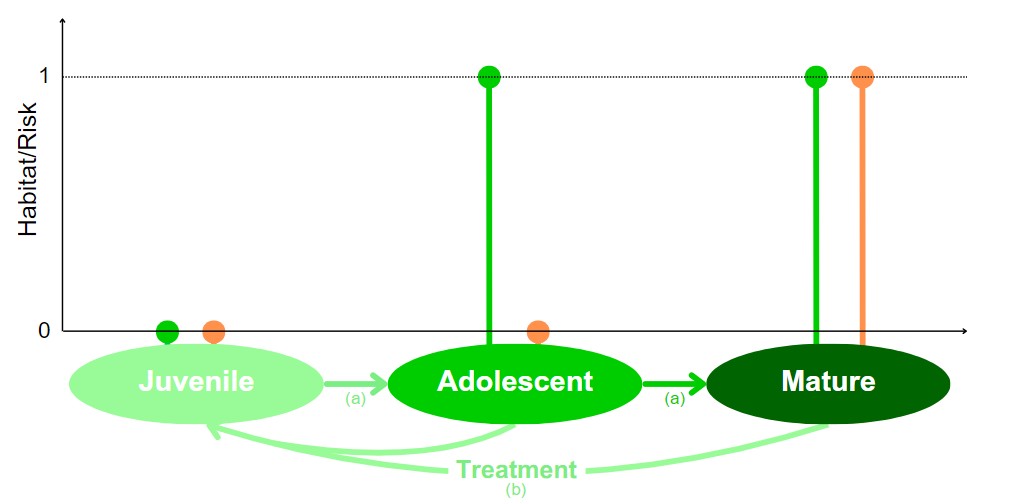
\includegraphics[width = .6\textwidth]{figures/wildland/Juvenile.png}
    \caption{Illustration of the successional stages and the link between successional stage, habitat and wildfire risk using a discretized Olson-type relationship}
    \subcaption*{At the bottom, the dynamics of the model are illustrated. First, successional stages transition (step (a)), then treatment is applied (step (b)). At the top, the link between successional stage, habitat and high risk. In green, a \textit{habitat} variables turns to $1$ when a cell is \textit{adolescent}, and in orange, a \textit{high risk} dummy turns to $1$ when a cell turns \textit{mature}} 
    \label{fig:illustration}
\end{figure}
%\end{minipage}%


%\subsection{Theoretical model}

We use a network structure to apprehend the landscapes. From the matrix $\mathbf{A}_t$, we form two graphs:  $\mathcal{B}_t = (V_{\mathcal{B}_t}, E_{\mathcal{B}_t})$, the graph of suitable habitat cells and $\mathcal{F}_t = (V_{\mathcal{F}_t}, E_{\mathcal{F}_t})$, the graph of high risk cells. First, the vertices of each graphs are the suitable habitat cells e.g $
V_{\mathcal{B}_t} = \{(i,j)$ such that $Habitat(a_{ijt})=1\}$ and the high risk cells, respectively e.g. $V_{\mathcal{F}_t} = \{(i,j)$ such that $Risk(a_{ijt})=1\}$.\\
Second, vertices are connected if they are within a Moore (or 8-cell) neighborhood of each other and share the same status. Therefore, notice that $\mathcal{F}_t\subset \mathcal{B}_t$. Figure \ref{fig:graph_overlap} illustrate the mechanism from the landscape in matrix form $\mathbf{A}_t$ with age classes ranging from 0 to 2, to graphs $\mathcal{B}_t$ and $\mathcal{F}_t$.

We use this 8-cell neighborhood for evaluating biodiversity habitat and wildfire risk within a common a spatial framework, using the same adjacency properties. 
Regarding biodiversity, we focus on general characteristics related to landscape structural connectivity rather than functional connectivity, as we are agnostic about effective species \citep{Fahrig2011}. We assume that species are able to disperse from one patch to another, and that habitat quality is uniformly distributed conditional on habitat being available.\\
We consider the wildfire risk through the lens of potential spread, influenced by fuel, wind direction and terrain. We abstract from wind patterns and terrain, to focus on fuel connectivity\footnote{Note that our framwork is amenable to prevailing wind patterns and terrain ruggedness, as the graph adjacency matrix can change from a Moore adjacency to any pattern influenced by environmental features}. Consistent with the literature (see \cite{Peterson_2009}, \cite{pais_cell2fire_2021, gonzalez-olabarria_fire_2023}), a wildfire can spread in any direction, conditional on neighbor cells with high risk. 

\begin{figure}
    \centering
    %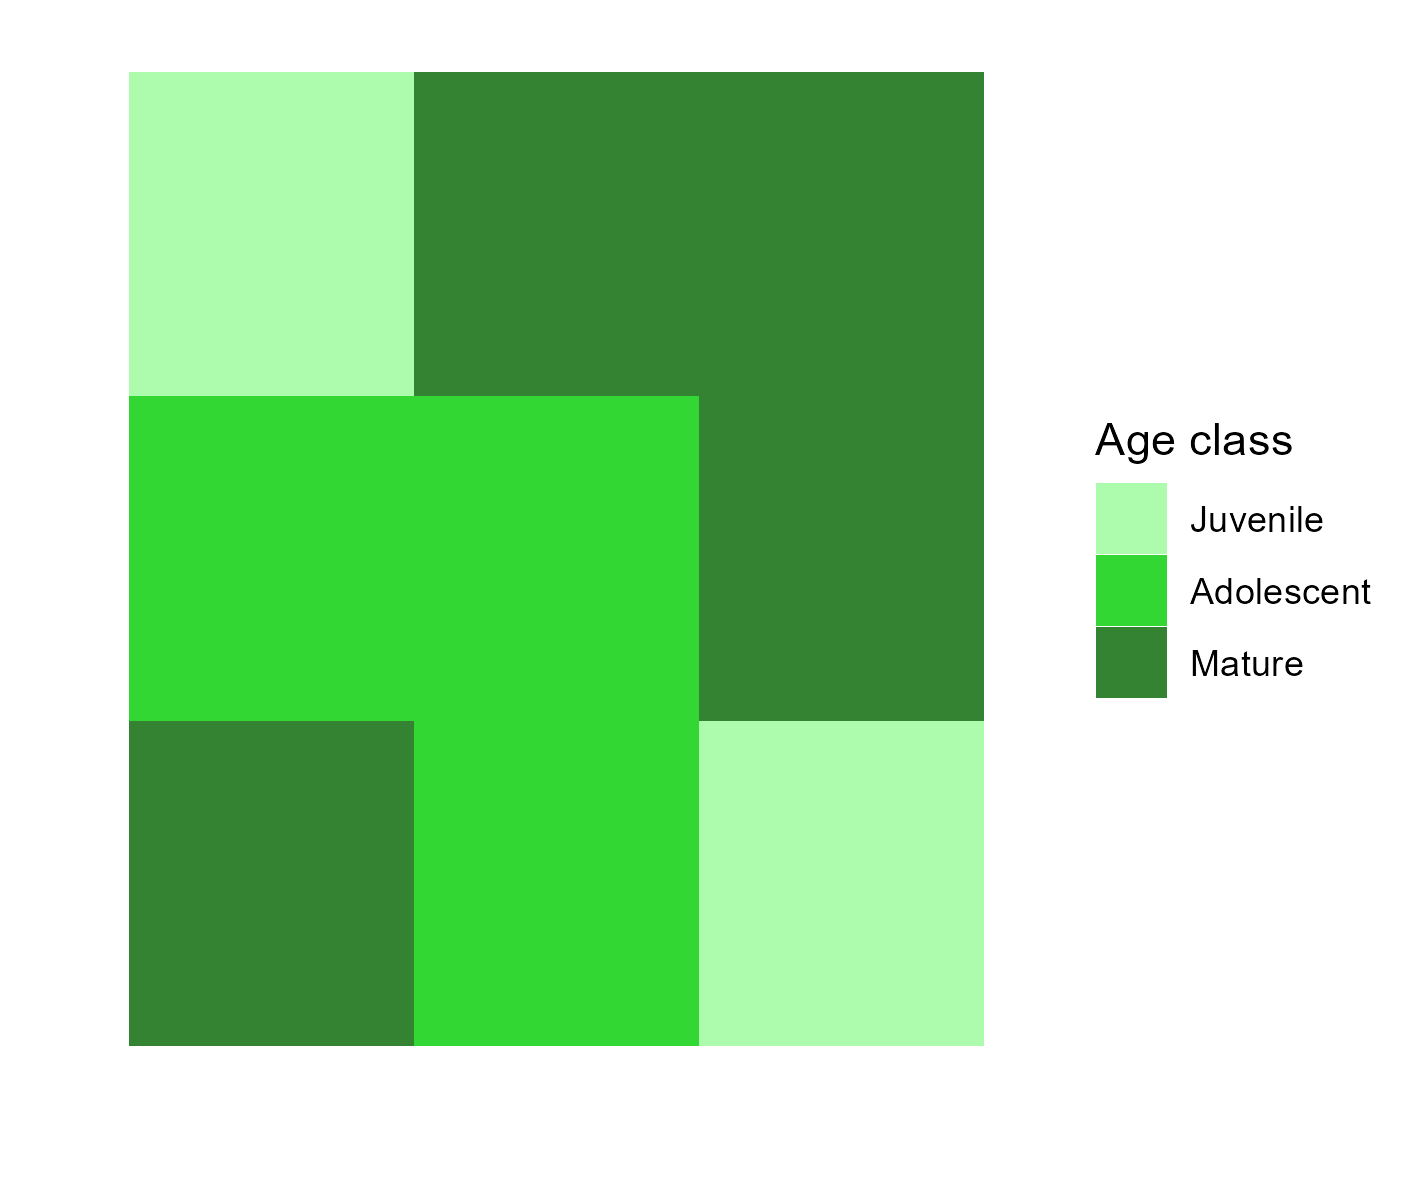
\includegraphics[width = .28\textwidth]{figures/wildland/illustration_from_raster.png}\\
    
\includegraphics[width = 0.2\textwidth]{figures/wildland/arrow_biod2.PNG}
    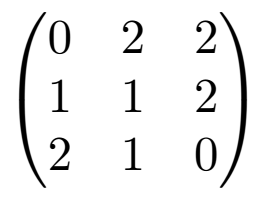
\includegraphics[width = 0.18\textwidth]{figures/wildland/land3.PNG}
    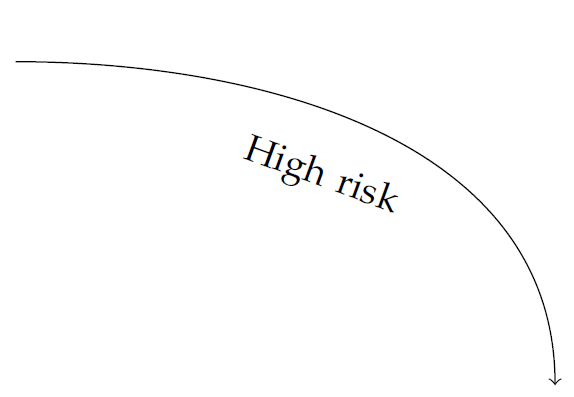
\includegraphics[width = 0.2\textwidth]{figures/wildland/arrow_fuel2.PNG}
    \\
    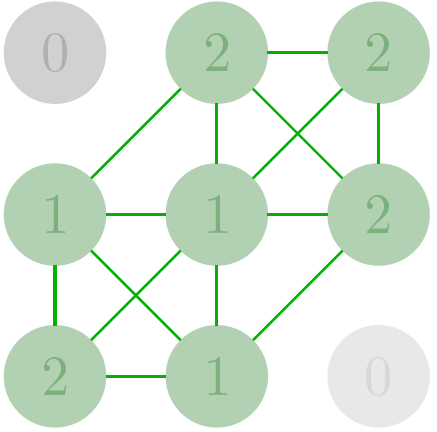
\includegraphics[width=0.2\textwidth]{figures/wildland/biodiv_3.PNG} \hspace*{4cm}
    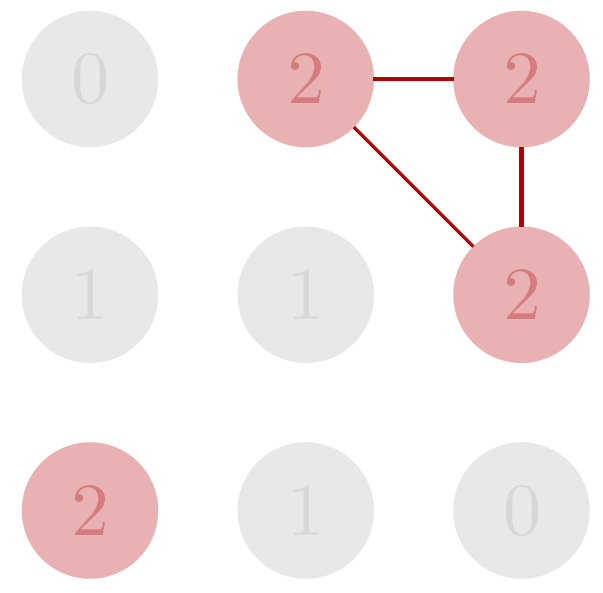
\includegraphics[width=0.2\textwidth]{figures/wildland/fire_3.PNG}\\
    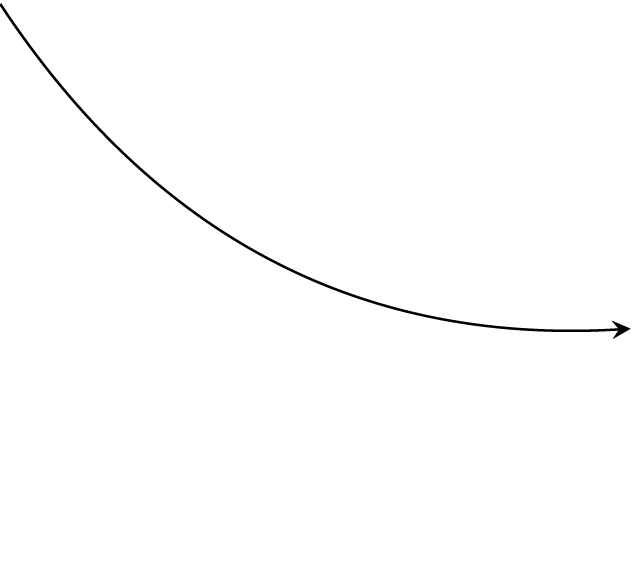
\includegraphics[width=0.18\textwidth]{figures/wildland/arrow_right.PNG}
    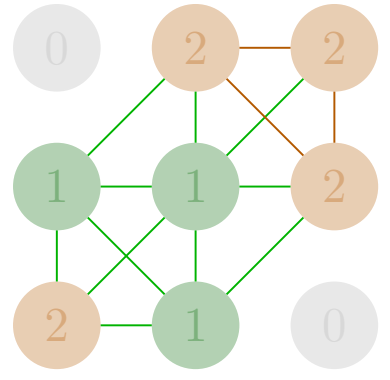
\includegraphics[width = 0.2\textwidth]{figures/wildland/graphe_feu_biod_33.PNG}
 	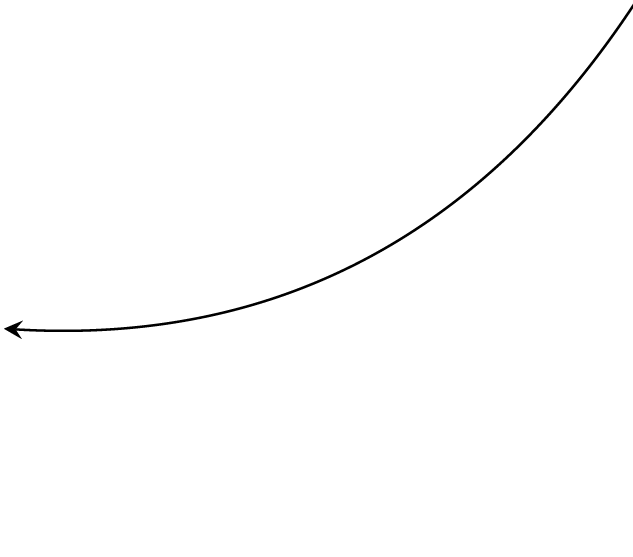
\includegraphics[width=0.18\textwidth]{figures/wildland/back_left.PNG}
    \caption{Illustration of the suitable habitat and high risk graphs for $n=3$}
    \subcaption*{The first layer is the values from a raster $\mathbf{A}_t$ of age classes in a forest landscape. It is turned into two different graphs. \\
In the left graph, the green vertices are $V_{\mathcal{B}_t}$ and support biodiversity habitat, while on the right graph, red vertices are $V_{\mathcal{F}_t}$ display high risk. Green and red links are respectively $E_{\mathcal{B}_t}$ and $E_{\mathcal{F}_t}$ \\
The high risk graph has two components (top right corner with 3 nodes, and bottom left corner with 1 node), while the biodiversity habitat graph only has one. \\
Cells for which the value is 0 are not considered as nodes for both graphs, and are thus not connected to the rest of the graphs. 
\\
In the final lansdcape, because $\mathcal{F}_t\subset \mathcal{B}_t$, the landscape  where orange cells are high fuel load and also support biodiversity habitat (e.g. $a_{ijt} \in V_{\mathcal{B}_t} \cap V_{\mathcal{F}_t}$)}
    \label{fig:graph_overlap}
\end{figure}

To assess the connectivity of $\mathcal{F}_t$ and $\mathcal{B}_t$, we use a global connectivity indicator. As connectivity can be measured in numerous ways in graph theory, we use this metric as is satisfies criteria pertaining to its evolution when vertices and edges are removed \citep{pascual-hortal_comparison_2006} when using graph theory applied to landscape ecology. Additionally, it offers a reformulation of the metric used in previous work closedly related to ours \citep{minas_spatial_2014, rachmawati_optimisation_2016} (see appendix \ref{sec:connectivity} for a demonstration). We define the global connectivity index of a given graph $\mathcal{G} = (\mathcal{V}, \mathcal{E})$ as\footnote{With $card$ being the cardinal operator in set theory and denotes the number of elements in a set}:
\begin{equation}
H(\mathcal{G}) = card(V) + 2card(E)
\label{eq:high_connectivity}
\end{equation} 
Let a \textit{patch} be a collection of connected cells of suitable wildlife habitat.
This indicator considers that a habitat cell is connected to itself (i.e, within a habitat patch, there is no barrier) and whether it is connected to other cells.  
It implies lower connectivity when the distance between habitat cells increases, attains its maximum value when a single habitat patch covers the whole landscape, indicates lower connectivity as the habitat is progressively more fragmented, considers negative the loss of a connected or isolated cell, and detects as more important the loss of bigger patch, and less important steppingstone cells or patches. 
\\
Our global connectivity indicator is similar to the notion of \textit{energy of a graph} \citep{gutman_energy_2001}, which can be understood as a measure of connectedness (highly connected graphs tend to have high energy) for graphs. However, we differ from \cite{gutman_energy_2001} by including self-loops as habitat cells and patches are connected to themselves. Our formulation of $H$ reframes a quadratic form from the adjacency matrix of a graph grid structure (appendix \ref{sec:connectivity}). The adjacency matrix displays interaction among nodes that are neither purely constructive or destructive, as some combinations of active neighboring nodes will add to global connectivity, while other combinations may substract global connectivity. In all the landscape sizes we used, eigenvalues of the adjacency matrix were both positive and negative, leading to indefiniteness (see figure \ref{fig:eigenvalues}). Therefore, $H$ is not globally convex nor concave. 
\\
%and The vertices of $\mathcal{B}_t$ are cells that are at suitable habitat status (e.g. $Habitat(a_{it})=1$ and high risk status (e.g. $Risk(a_{it})=1$) and suitable habitat status
%
%We transform $A_t$ the set of cells constituting the landscape into graphs $G_t$ whose vertices $V_t$ (or nodes) are the cells in the landscape, and edges $E_t$ represent the connections between cells. We partition the landscape in two graphs, $G_{B_t}$ and $G_{F_t}$, each describing the network of mature habitat and risky patches (see fig. 1 for a representation). Landscape ecology has long used numerous, theoretically grounded indicators to analyze landscapes 
%
%\citep{urban_landscape_2001,minor_graph-theory_2008}. We use a global connectivity indicator that satisfies \cite{pascual-hortal_comparison_2006} criteria, grounded in graph theory, that offer a reformulation of \cite{rachmawati_optimisation_2016} (see Appendix \ref{sec:connectivity}). 
%Figure reference : \ref{fig:graph_overlap}
%
%We define cells to be connected if (i) they are within an 8-cell neighborhood and (ii) share the same status e.g. for a cell $i$, if cell $j$ is an 8-cell neighborhood (should we define it?)
%
%We define the global connectivity index of habitat and risky patches in landscape $A(t)$ as:
%
%This indicator considers that a habitat patch is connected to itself (i.e, within a habitat patch, there is no barrier) and whether it is connected to other patches.  
%It implies lower connectivity when the distance between patches increases, attains its maximum value when a single habitat patch covers the whole landscape, indicates lower connectivity as the habitat is progressively more fragmented, considers negative the loss of a connected or isolated patch, and detects as more important the loss of bigger patches, of key and less important steppingstone patches.
%
%We use a connectivity matrix to evaluate the ladnscape such that ...
%\textit{note that the framework is robust to changing the dispersal abilities. For example, one could think of (i) changing the dispersal abilities and (2) increase the size of the landscape to run applied stuff and (3) finding metrics to prioritize over species with different dispersal abilities. \textbf{This is a good discussion point : next work should include a variety of dispersal abilities and contributions to functional diversity to really dig deeper in this issue. }}
%\\\\

\subsection{Social planner decision : the high-risk /connectivity dilemma}
\subsubsection{Dynamic decision problem}
A social planner tries to minimize the global connectivity index of the high risk graph, using fuel treatments (eq. \ref{eq:objective}). However, when implementing treatment, a cell's successional stage is reset to \textit{juvenile}, thus destroying biodiversity habitat. In coherence with real world applications, the social planner is faced with a temporal budget constraint (e.g. the sum of treatments $\sum_{ij}x_{ijt}$ must be lower or equal to the $Budget$ - eq. \ref{const:budget}) as well as an ecological constraint, in terms of biodiversity habitat connectivity (e.g. the global connectivity of biodiversity habitat $H(\mathcal{B}_t)$ must be larger than constraint $Biod$ - eq. \ref{constr:biod}). Both the ecological and budget constraint need to be satisfied in each period.
\\
For the sake of the analysis, we focus on two layers of complexity : time and space. We do not include a stochastic component related to wildfire risk e.g. we adopt a deterministic framework where the value at risk (global connectivity of risky cells) is weighed against the loss in biodiversity habitat connectivity. Additionally, we consider a homogeneous distribution of treatment costs across the landscape e.g. cost of treatment in each cell through time is $1$. We come back to this assumption in the discussion. Monetary benefits are also homogenously distributed across the landscape, and normalized to 1. Note that there is, however, heterogeneous returns to treating across the landscape : some cells will contribute more than other to global connectivity. Finally, given that the planning horizon is finite, we do not discount future high risk connectivity scores and assume each period is equally important in decision making.

The optimization problem is : 

\begin{align}
    \min_{ \{\{x_{ijt}\}_{(i,j)}\}_{t=1}^T} & \left[ \sum_{t=1}^T H(\mathcal{F}_t)\right] \label{eq:objective}\\
\text{Such that: } & \notag \\
\mathbf{A}_0 &\text{ given} \label{eq:init_cond}\\
\forall t \in \{1, ..., T\} : & \notag \\
H(\mathcal{B}_t)&\geq Biod,\text{  }\label{constr:biod}\\
\text{ and }\forall (i,j) \in \{1,...,n\}   :& \notag \\
a_{ijt+1}& = \min((a_{ijt+1}(1-x_{ijt});2), \label{const:dyn}\\
 \sum_{i,j} x_{ijt} & \leq Budget,\text{  } \label{const:budget}\\
x_{ijt}&\in \{0,1\}\label{const:control}
\end{align}

\begin{table}[h]
\centering
\onehalfspacing
\begin{tabular}{|c|c|}
\hline
Notation & Concept \\
\hline \hline
$\mathbf{A}_t$ & Landscape matrix representing successional stage at time $t$ \\
$a_{ijt}$ & Cell $(i,j)$ of landscape with value $\in \{0,1,2\}$\\ 
$x_{ijt}$ & Treatment status $\in\{0,1\}$ of cell $(i,j)$ at time $t$ \\
$H$ & Global connectivity measure\\
$\mathcal{F}_t = (V_{\mathcal{F}_t}, E_{\mathcal{F}_t})$ & Graph of high risk cells\\
$\mathcal{B}_t = (V_{\mathcal{B}_t}, E_{\mathcal{B}_t})$ & Graph of suitable habit cells\\
\hline \hline
$Biod \in \{0,...,\max H(\mathcal{B})\}$ & Level of habitat global connectivity constraint\\
$Budget \in \{1,2,3,4\}$ & Level of the budget constraint\\
$n \in \{3,4,100\}$ & Size of the lansdcape\\
$c = 3$ & Number of age classes \\
$T \in \{5,10\} $ & Planning horizon\\
\hline 
\end{tabular}
\caption{Summary of model variables and functions}
\end{table}
%There are several reasons for this choice. First, the complexity of our problem is increasing in space and time, and in the number of initial conditions, as interpolation in a spatial setting is difficult given the behavior of our objective function. 
As common in the literature, we can express the budget as a share of land being treated ranging from 10\% to 33\% of the surface area (when $n=3$) and 5 to 25\% of the surface area (when $n=4$). These values encompass historical and projected policies in Australia \citep{burrows2013}, the United States \citep{GAO2019} and Southern Europe \citep{Fernandes2013}.
\\
Additionally, we solve the problem for a range of possible habitat connectivity values, ranging from $0$ to the maximum possible habitat connectivity for each landscape size $n$.

\subsubsection{Non-convexity and dimensionality curse}
Our problem can be classified as a \textit{critical node detection problem}, i.e, a problem of locating the vertices that best degrade our global connectivity metric $H(\mathcal{F}_t)$ \citep{ARULSELVAN20092193}. Problems of the critical node class are computationally difficult (e.g. NP - Hard) in a single graph \citep{ARULSELVAN20092193, matsypura_wildfire_2018}. Efficient heuristics to find near-optimal solutions exist and leverage perturbations around local solutions \citep{ARULSELVAN20092193, Zhou2017}. Compared to the canonical \textit{critical node detection} problem, our problem features a non-convex objective function, a budget constraint, and a constraint on habitat connectivity, which imposes a constraint on the supergraph of high risk cells. Given our constraints, the behavior of the global connectivity measure $H$, standard optimization techniques cannot be applied, and heuristics are required. \\
%We solve the dynamic, integer program of the landscape manager
In dynamic problems, a standard technique is dynamic programming \citep{Bellman}. Dynamic programming provides a temporal decomposition of the initial problem defined over $T$ periods, into $T$ recursive problems, as it relies on the 'optimality principle'\footnote{"An optimal policy has the property that whatever the initial state and initial decision are, the remaining decisions must constitute an optimal policy with regard to the state resulting from the first decision". (See \cite{Bellman}, Chap. III.3., p.83)"}. A value function $V$, mapping each possible state of the world e.g. $\mathbf{A}_t$ to the optimal value of the objective function along the planning horizon, is iterated upon to find the optimal policies $x_{ijt}^*(\mathbf{A}_t)$, i.e, the sequence of optimal treatments, and the optimal states $\mathbf{A}_t^*(\mathbf{A}_0)$ resulting from the optimal policies and the initial conditions.
However, it is impractical in our case. Our problem suffers a \textit{dimensionality curse} \citep{Bellman}. There are $3^{n^2}$ values for the state variables \footnote{Given that the landscape $\mathbf{A}$ is of size $n\times n$, and that each element of $a_{ij}$ can take $c=3$ values, there are $3^{n^2}$ landcape configurations possible} in each period and the specific nature of our objective function $H$, the habitat connectivity and budget constraints make interpolation of a value function impossible \footnote{As a matter of fact, with a large number of state variables e.g. a high-dimensional state space, methods such as adaptive sparse grids can be used towith smooth, continuous objective functions \citep{brumm_adaptive_2017} to circumvent the dimensionality curse. The fact that the input space is an $n^2$-dimensional binary Cartesian product and that $H$ is not globally convex hinder the use of such tools.}.
%To manage the expected damages resulting from wildfires, the land planner can decide to undertake specific treatments, in the form of a combination of controlled burns and/or mechanical thinnings. Upon treatment, we assume that vegetation age in the cell is reset to 'absent': the wildfire risk vanishes, but so does the habitat and its connection to surrounding cells. Given the tension between maintaining habitat and reducing wildfire risk, the land planner aims to minimize a deterministic measure of connectivity of the high fuel loads in the landscape while maintaining a given level of biodiversity habitat connectivity under a budget constraint, over a planning horizon of length $T$. 
%For the sake of the analysis, we focus on two layers of complexity over time and space: global connectivity of high risk and biodiversity habitat. We do not consider stochastic wildfire behavior\textbf{point on risk and expected utility? } , heterogeneity in the economic costs or benefits (i.e, homogeneous treatment costs and no patch-specific asset to protect). The framework is however amenable to such a prioritization. We also assume that the budget cannot be banked, and has to be utilized in each period, consistent with operational rules. Moreover, as the budget is constrained in each period, the measure of risk is bounded and the planning horizon is finite, we rule out discounting and assume each generation matters as much to the social planner. 
%We abstract from decision-making in a risky environment, as it has been extensively described in economics and decision theory \citep{Mouysset2013}. Moreover, we mimic the role of risk aversion by varying the level of habitat connectivity constraint the decision maker chooses. 
%If ignition is a binary process in each period, the probability of which is independent of the high-risk graph properties, our model can be viewed as minimizing an upper bound of the expected losses from wildfires (see appendix).


\subsection{Solution method and computational experiments}

Three key features of our problem hint that a dynamic (e.g. that optimizes the objective function over the whole planning horizon) and a repeated myopic solution (e.g. which optimizes the objective function in each period)  should be similar. The dynamics occur before the decision is made, therefore the decision maker has full knowledge about the state of the system. The dynamics are simplified and have relatively little depth, as we limit ourselves to 3 age classes. Finally, our intertemporal objective function is additively separable.

Our solution methods resorts to two key ingredients : optimization heuristics, and comparison between the dynamic and repeated myopic problem. \\
First, we circumvent the non-convexity of the global connectivity metric and the high dimension of the state space by using a genetic algorithm \citep{holland_adaptation_1975} (implemented in \textsf{R} with package \textit{GA} \citep{GA_2017}) for 300 randomly generated landscapes, with population size of $200$ and $250$ iterations. Genetic algorithms are especially suited for high dimensional, combinatorial search spaces\footnote{Here, the control variable is a $Tn^2 = 5n^2$ binary variable} and fare better than a brute force approach, or other heuristics (Particle Swarm Optimization or Simulated Annealing). 
\\
Then, we compare the performance of a 5-period objective function to a 5 period repetition of a static objective function. We trade the completeness of dynamic programming for a more manageable approach, where we compare these approaches for $696$ and $884$ randomly drawn landscapes of size $n \in \{3,4\}$. We sample the landscapes according to the distribution of possible landscapes (see figure \ref{fig:appendix_distribution}). As landscapes with large numbers of \textit{juvenile} and \textit{adolescent} cells are overrepresented, we impose that underrepresented possible landscapes are included at least 2 times in our sample, to disentangle composition (e.g. number of cells of each successional stage) from configuration (location of cells) effects.

 We focus $T=5$ planning horizon for several reasons. First, as the dynamic of our ecological processes comprises 3 stages, using a 5-period horizon allows for each cell to grow from its original stage to \textit{mature}, be treated, and revert to its original stage, e.g. allows for a full successional cycle to be performed. Second, a 5-period horizon corresponds to a long policy horizon, ranging from 25 years to 200 years \citep{mccoll_gausden_pathways_2019, thomas_wildlife_1979}.
Third, for our approach to be useful for policy making given that we abstract from stochastic modifications to the environment (e.g. occurence of wildfire, spread of invasive species increasing flamability at a given age etc), policies need to be forward looking with enough temporal depth to be relevant and be reevaluated with potentially new initial conditions resulting from environmental perturbations.\\
Next, we increase the size of our sample with repeated static optimization and temporal depth, to encompass all the possible landscape configurations for landscape size $n \in \{3, 4\}$, over the whole range of possible values for the biodiversity habitat constraint, over $T=10$ years. 
Of all the $3^{n^2}$ initial landscapes combinations possible, we only keep landscapes that are unique up to a permutation\footnote{That is to say, landscape $\mathbf{A}_0$ is included in the set of initial conditions $\mathcal{I}$ if and only if for any element $\mathbf{A'}_0$ in $\mathcal{I}$, $\mathbf{A}_0$ is not a permutation (eg can be obtained through rotations or symmetries) of $\mathbf{A'}_0$}. This results in a sharp reduction of landscapes to consider, from $19,683$ initial conditions to $2861$ unique initial landscapes for $n=3$, and from $43,046,721$ initial to $5,398,082$ unique initial landscapes for $n=4$. We focus on exact optimal solutions for all the initial conditions of these small-scale landscapes and implement our own solution algorithm in Python 3.9.13 and R 4.3.3\footnote{Data and code are \href{https://github.com/sim-jean/Landscape_connectivity_dilemma}{publicly available}}.
\\
Third, we increase the landscape size to $n=100$, for a sample of 20 large scale (10,000 cells) landscapes with varying compositions and autocorrelation using two-dimensional fractional Brownian motions  (table \ref{tab:composition_nlm} summarizes their characteristics and figure \ref{fig:ex_nlm} illustrates 6 of them). We use neutral landscape models \citep{caswell_community_1976, gardner_neutral_2007} and implement them in \textsf{R} \citep{sciaini_nlmr_2018}. Neutral landscape models were designed in theoretical landscape ecology to develop spatial ecology indicators and ``evaluate the effects of landscape structure on ecological processes'' \citep{with_neutral_1997}. Even though they are designed as null models to compare with real landscapes, after ecological processes have shaped them, they provide a useful basis for scaling our analysis. We solve the repeated myopic optimization problem on these 20 landscapes over $T=10$ periods.\\
%
%
%\subsubsection{Non-convexity and dimensionality curse}
%Our problem can be classified as a \textit{critical node detection problem}, i.e, a problem of locating the vertices that best degrade our global connectivity metric $H(\mathcal{F}_t)$ \citep{ARULSELVAN20092193}. Problems of the critical node class are computationally difficult (e.g. NP - Hard) in a single graph \citep{ARULSELVAN20092193, matsypura_wildfire_2018}. Efficient heuristics to find near-optimal solutions exist and leverage perturbations around local solutions \citep{ARULSELVAN20092193, Zhou2017}. Compared to the canonical \textit{critical node detection} problem, our problem features non-convex objective function, a budget constraint, and a constraint on habitat connectivity, which imposes a constraint on the supergraph of high risk cells. Given our constraints, the behavior of the global connectivity measure $H$, standard optimization techniques cannot be applied. \\
%We solve the dynamic, integer program of the landscape manager
%In dynamic problems, a standard technique is dynamic programming. Dynamic programming provides a temporal decomposition of the initial problem defined over $T$ periods, into $T$ recursive problems, as it relies on the 'optimality principle'\footnote{"An optimal policy has the property that whatever the initial state and initial decision are, the remaining decisions must constitute an optimal policy with regard to the state resulting from the first decision". (See \cite{Bellman}, Chap. III.3., p.83)"}. A value function $V$, mapping each possible state of the world e.g. $\mathbf{A}_t$ to its objective function value, is iterated upon to find the optimal policies $x_{ijt}^*(\mathbf{A}_t)$, i.e, the sequence of optimal controlled burns, and the optimal states $\mathbf{A}_t^*(\mathbf{A}_0)$ resulting from the optimal policies and the initial conditions.
%However, it is impractical in our case. As a matter of fact, our problem suffers a \textit{dimensionality curse} \citep{Bellman}. There are $3^{n^2}$ possible combinations\footnote{Given that the landscape $\mathbf{A}$ is of size $n\times n$, and that each element of $a_{ij}$ can take $c=3$ values, there are $3^{n^2}$ landcape configurations possible} in each period and the specific nature of our objective function $H$, the habitat connectivity and budget constraints make interpolation of a value function impossible \footnote{As a matter of fact, even with a large number of state variables e.g. a high-dimensional state space, adaptive sparse grids can be used with smooth, continuous objective functions \citep{brumm_adaptive_2017}. The fact that the input space is an $n^2$-dimensional binary Cartesian product and that $H$ is not globally convex hinder the use of such tools.}. 
%
%Nonetheless, three key features of our problem hint that dynamic and repeated myopic solutions should be similar. The dynamics occur before the decision is made, therefore the decision maker has full knowledge about the state of the system. The dynamics are simplified and have relatively little depth, as we limit ourselves to 3 age classes. Finally, our intertemporal objective function is additively separable.
%
%
%
%\subsubsection{Dynamic v. repeated myopic solutions}
% 
%To circumvent this issue, we adopt a three-fold approach. \\
%First, we trade the completeness of dynamic programming (e.g. solution of the problem for the entire domain of the state variable $\mathbf{A}$) for a manageable piecemeal approach, where we solve the complex 5-period combinatorial problem with a genetic algorithm \citep{holland_adaptation_1975} (implemented in \textsf{R} with package \textit{GA} \citep{GA_2017}) for 300 randomly generated landscapes, with population size of $200$ and $250$ iterations. Genetic algorithms are especially suited for high dimensional, combinatorial search spaces\footnote{Here, the control variable is a $Tn^2 = 5n^2$ binary variable} and fare better than a brute force approach, or other heuristics (Particle Swarm Optimization or Simulated Annealing). 
%
%Three key features of our problem hint that dynamic and repeated myopic solutions should be similar. The dynamics occur before the decision is made, therefore the decision maker has full knowledge about the state of the system. The dynamics are simplified and have relatively little depth, as we limit ourselves to 3 age classes. Finally, our intertemporal objective function is additively separable.
%Hence, we compare the performance of the 5 period, genetic algorithm approach to a repeated static optimization procedure, for landscapes of size $n\in\{3,4\}$. While this size appears simplifying, it encapsulates the main mechanisms displayed in similar models \citep{rachmawati_optimisation_2016, rachmawati_fuel_2018}. Based on these results, we increase the planning horizon to
%\\
%\textbf{Comment est ce qu'on dit ici qu'on accroit peut être l'horizon?}
%Second, we perform a repeated static optimization on all the possible landscape configurations for landscape size $n \in \{3, 4\}$, over all the whole range of possible values for the biodiversity habitat constraint, over 5 years. This approach sacrifices the dynamics of our problem but allows us to scan the entire state space to gain insights.
%Of all the $3^{n^2}$ initial landscapes combinations possible, we only keep landscapes that are unique up to a permutation\footnote{That is to say, landscape $\mathbf{A}_0$ is included in the set of initial conditions $\mathcal{I}$ if and only if for any element $\mathbf{A'}_0$ in $\mathcal{I}$, $\mathbf{A}_0$ is not a permutation (eg can be obtained through rotations or symmetries) of $\mathbf{A'}_0$}. This results in a sharp reduction of landscapes to consider, from $19,683$ initial conditions to $2861$ unique initial landscapes for $n=3$, and from $43,046,721$ initial to $5,398,082$ unique initial landscapes for $n=4$. We focus on exact optimal solutions for all the initial conditions of these small-scale landscapes and implement our own solution algorithm in Python 3.9.13 and R 4.3.3\footnote{Data and code are \href{https://github.com/sim-jean/Landscape_connectivity_dilemma}{publicly available}}.
%\\
%Third, we simulate 20 large scale (10,000 cells) landscapes with varying compositions and autocorrelation using two-dimensional fractional Brownian motions  (table \ref{tab:composition_nlm} summarizes their characteristics and figure \ref{fig:ex_nlm} illustrates 6 of them). We use neutral landscape models \citep{caswell_community_1976, gardner_neutral_2007} and implement them in \textsf{R} \citep{sciaini_nlmr_2018}. Neutral landscape models were designed in theoretical landscape ecology to develop spatial ecology indicators and ``evaluate the effects of landscape structure on ecological processes'' \citep{with_neutral_1997}. Even though they are designed as null models to compare with real landscapes, after ecological processes have shaped them, they provide a useful basis for scaling our analysis. We solve the repeated myopic optimization problem on these 20 landscapes.
%
%using dynamic programming. Dynamic programming provides a temporal decomposition of the initial problem defined over $T$ periods, into $T$ recursive problems, as it relies on the 'optimality principle'\footnote{"An optimal policy has the property that whatever the initial state and initial decision are, the remaining decisions must constitute an optimal policy with regard to the state resulting from the first decision". (See \cite{Bellman}, Chap. III.3., p.83)"}.  The outputs of the method are both the optimal policies $x_j^*(t,A)$, i.e, the sequence of optimal controlled burns, and the optimal states $A_j^*(t,A_0)$ resulting from the optimal policies and the initial conditions. Moreover, we solve a repeated myopic optimization procedure, where in each time step, the decision maker minimizes the current global connectivity measure of high risk cells, under constraints \ref{eq:init_cond}-\ref{const:control}. In the dynamic problem, the biodiversity habitat and budget constraints gradually restrict the solution space, and limit the extent to which system dynamics (e.g the appraisal of long terms successional stages across the landscape) may impact optimal solutions. We compare the repeated myopic solution to the dynamic solution.
%
%\subsubsection{Circumventing non-convexity and dimensionality curse}
%
%Our problem can be classified as a \textit{critical node detection problem}, i.e, a problem of locating the vertices that best degrade our global connectivity metric $H(\mathcal{F}_t)$ \citep{ARULSELVAN20092193}. Problems of the critical node class are computationally difficult (e.g. NP - Hard) in a single graph \citep{ARULSELVAN20092193, matsypura_wildfire_2018}. Efficient heuristics to find near-optimal solutions exist and leverage perturbations around local solutions \citep{ARULSELVAN20092193, Zhou2017}. Our problem is a constrained, integer optimization problem with a non-convex objective function,
%that constrains not only the set of nodes to be removed but also metrics relative to a larger graph structure e.g. the supergraph of high risk cells, biodiversity habitat. Given the behavior of the global connectivity measure $H$, standard optimization techniques cannot be applied. \\
%Additionally, the complexity of our combinatorial problem increases with landscape size $n$, the number of vegetation age classes $c$, and time $T$ i.e. features a \textit{dimensionality curse} \citep{Bellman}: there are $c^{n^2}$ eg. $3^{n^2}$ initial landscape configurations possible, and given an initial landscape, there are $n^2 \times T$ possible treatment allocations to be considered. 
%To circumvent these issues, we use a genetic algorithm \citep{holland_adaptation_1975} (implemented in \textsf{R} with package \textit{GA} \citep{GA_2017}). Compared to other heuristics, such as Particle Swarm Optimization or Simulated Annealing, genetic algorithms fare better on high dimension, combinatorial search spaces. With small scale landscapes (e.g. $n\in \{3,4\}$), we use a population size of $100$ individuals with $250$ iterations which guarantees that the heuristic converges to a near optimal solution.
%
%Moreover, as the objective function is neither globally convex nor concave, and the structure of the optimization problem is constrained, we required large test populations for our genetic algorithm to avoid getting stuck in local minima.  es.
%
%\subsubsection{Small and large scale repeated myopic optimization}
%
%We limit ourselves to studying the initial conditions in landscapes of size $n=3$ and $4$. While this formulation appears simplifying, it encapsulates the main mechanisms displayed in similar models \citep{rachmawati_optimisation_2016, rachmawati_fuel_2018}.\\
%First, we solve the dynamic problem and repeated static problem for 300 randomly selected initial landscapes.
%Then, we focus on all the possible landscape combinations of size $n \in \{3,4\}$ using repeated myopic optimization, over all the whole range of possible values for the biodiversity habitat constraint, over 5 years. \\
%Of all the $3^{n^2}$ initial landscapes combinations possible, we only keep landscapes that are unique up to a permutation\footnote{That is to say, landscape $\mathbf{A}_0$ is included in the set of initial conditions $\mathcal{I}$ if and only if for any element $\mathbf{A'}_0$ in $\mathcal{I}$, $\mathbf{A}_0$ is not a permutation (eg can be obtained through rotations or symmetries) of $\mathbf{A'}_0$}. This results in a sharp reduction of landscapes to consider, from $19,683$ initial conditions to $2861$ unique initial landscapes for $n=3$, and from $43,046,721$ initial to $5,398,082$ unique initial landscapes for $n=4$. We focus on exact optimal solutions for all the initial conditions of these small-scale landscapes and implement our own solution algorithm in Python 3.9.13 and R 4.3.3\footnote{Data and code are \href{https://github.com/sim-jean/Landscape_connectivity_dilemma}{publicly available}}.
%
%
%
%Finally, we simulate 20 large scale (10,000 cells) landscapes with varying compositions and autocorrelation using two-dimensional fractional Brownian motions  (table \ref{tab:composition_nlm} summarizes their characteristics and figure \ref{fig:ex_nlm} illustrates 6 of them). We use neutral landscape models \citep{caswell_community_1976, gardner_neutral_2007} and implement them in \textsf{R} \citep{sciaini_nlmr_2018}. Neutral landscape models were designed in theoretical landscape ecology to develop spatial ecology indicators and ``evaluate the effects of landscape structure on ecological processes'' \citep{with_neutral_1997}. Even though they are designed as null models to compare with real landscapes, after ecological processes have shaped them, they provide a useful basis for scaling our analysis. We solve the repeated myopic optimization problem on these 20 landscapes.
%
%
\subsection{Lanscape indicators}
\label{section:indicators}
To characterize the managed landscapes, we mobilize several indicators from landscape ecology and graph theory (see appendix \ref{sec:appendix_wildland__indicators}).

First, we account for the high risk and habitat surfaces in the landscape by measuring the number of vertices in each graph.
Second, to assess landscape connectivity and fragmentation as well as landscape diversity\footnote{In the context of fire prone ecosystems, the notion of ``fire mosaics'' \citep{bradstock_which_2005} conveys the idea that fire causes variations in successional stages through space thus providing different types of habitat for biodiversity and improving biodiversity}, we use our global connectivity metric $H$ (eq. \ref{eq:high_connectivity}), as well as the \textit{number of components}\footnote{A \textit{component $\mathcal{C}_t$} of graph $\mathcal{G}_t$ is a maximally connected subgraph of $\mathcal{G}_t$ that is not part of any larger connected subgraph. A component is \textit{connected} (for all two vertices $(u,v) \in V_{\mathcal{C}}$, there exists a path in $\mathcal{C}_t$ that connects them) and $\mathcal{C}_t$ being a subgraph of $\mathcal{G}_t$, it is \textit{maximal} if there is no other connected subgraph $\mathcal{C'}$ of $\mathcal{G}_t$ such that $\mathcal{C}_t$ is a proper subgraph of $\mathcal{C'}_t$. Figure \ref{fig:graph_overlap} illustrates this concepts in both the habitat and high risk graphs resp. $\mathcal{B}_t$ and $\mathcal{F}_t$}.
To specifically assess landscape diversity, we use the Simpson index \citep{simpson_measurement_1949} on successional stages stages (eq. \ref{eq:simpson})\footnote{Similar results can be found with the Shannon index \citep{Shannon1949}. To avoid issues related to degenerate values and logarithms, we focus on the Simpson index.}. 
However, the Simpson index does not account for the diversity of spatial patterns: a checkered landscape with two seral stages would be as diverse as a landscape with two large patches for each seral stage, according to the Simpson index. Therefore, we use the landscape shape index (eq. \ref{eq:LSI}), a normalized ratio between the perimeter of biodiversity habitat and its area \citep{patton_diversity_1975, McGarigal_1995}.
%\begin{equation}
%LSI = \frac{perimeter(\mathcal{G}_t)}{4n} \text{ such that }\mathcal{G}_t \in \{\mathcal{B}_t,\mathcal{F}_t\}
%\end{equation}
To disentangle the correlated effects of perimeter and area that affect the landscape shape index, we use a successional stage heterogeneity index, that averages the probability that, for each cell, neighbors in the 4 cardinal directions share the same successional stage (eq. \ref{eq:lth_index}). The index ranges between 0, when the successional stage is the same across the whole landscape, to 1, in a checkered landscape. The index assesses whether the landscape is a mosaic \citep{bradstock_which_2005}, and if it displays structural diversity, conducive to diverse communities and functional diversity. 

\section{Results}
\label{section:results}
\begin{itemize}
\item Need to rethink the argument in terms of steady states
\\
$\Rightarrow$ We no longer can use this argument because we sacrificed the duration
\item We want to characterize the long term trajectories with $T=5$?
\item What can we do?
\end{itemize}
\subsection{Steady states}
Our simulations show that 100\% of the initial landscapes converge in finite time towards a steady state solution, that minimizes wildfire risk while satisfying budgetary and habitat connectivity requirements. Steady states are landscape cycles with finite periods. Analyzing the steady-state cycles (and the unique landscapes that form them) drastically reduces the set of landscapes to analyze: they represent 2\% (resp. $0.001\%$) of the initial landscapes of size $n=3$ (resp. $n=4$). Our model highlights the convergence of landscapes towards types that can be managed to deliver several objectives. As landscape size increases, the number of steady state landscape cycles increases, but the power of convergence increases as well (e.g. ratio between initial configurations and effective steady state landscapes): from 19 683 initial landscapes when $n=3$, 51 steady states emerge and from 43 046 721 initial landscapes when $n=4$, at most 95 diverse steady-state landscapes emerge. Focusing on steady states makes all the more sense as landscape size increases. 

Eventually, figure \ref{fig:distrib_cycles} shows that conditional on data availability on every patch, the more the decision maker wants to conserve biodiversity, the fewer steady-state landscapes she has to consider. An increase in the habitat requirement reduces the room for maneuver. Indeed, budget acts as a complexifying factor: the larger the budget (relative to costs), the larger the set of steady-states to consider. 
%Our results show that habitat connectivity can be an objective and serve as an information cost-saving strategy. Data on the status of land patches gets cheaper to acquire with remote-sensing strategies, and random environmental factors can perturb optimal trajectories.
Aiming for relatively large habitat connectivity reduces the set of viable strategies to be considered and can more efficiently guide policy. 

\subsection{Wildfire risk reduction and habitat connectivity in steady state landscapes}

Figure \ref{fig:frontier} shows the wildfire risk reductions and habitat requirements normalized by their respective maximum values for landscapes of size $n=3$ and $4$. The maximum value for both risk and habitat corresponds to a landscape covered in 'old' vegetation, which we take to be the counterfactual. 
Randomly assigned treatments do generate risk reductions but are not cost nor habitat-efficient. Following our spatial optimization procedure, it is clear that implementing fuel treatment reduces wildfire risk while supporting biodiversity habitat. Figure \ref{fig:frontier} shows that these two objectives come as a trade-off, albeit moderate: indeed, increasing habitat requirements increases the remaining risk, but there are combinations that can satisfy large habitat connectivity and risk reductions. 
Budget is a key factor in risk reduction, as it relaxes the trade-off between the two objectives: increasing the budget reduces the wildfire risk while maintaining a range of biodiversity constraints. When habitat constraints are large, however, the marginal effect of budget is limited, and a larger remaining risk needs to be accepted. For example, with a budget of 25\% of land to be treated (with landscape size $n=4$), and no habitat constraint, risk can be reduced up to 80\% compared to the counterfactual scenario. However, when the habitat constraint is at 60\%, only 70\% of risk reduction can be achieved. Moreover, this risk reduction can be achieved with a lower budget. Conversely, as the costs of treatment increase, for a stable budget, the remaining risk increases sharply, and factoring in habitat requirements in the decision-making is not necessary for targets below 80\%. 
%\textbf{Pas sur de ça, un peu gros peut être?} Our results suggest that in the face of climate change if treatment costs increase, focusing on reducing wildfire risk should be a priority and would accommodate wildlife habitat. 
%\textbf{Point sur l'importance de la spatialisation? i.e, meilleur score vs random? ou focus sur un seral stage?}

\subsection{Properties of steady state landscapes: surface, fragmentation, and diversity}
Figure \ref{fig:cycles_3_4} displays, for each class, the most frequent steady-state cycle for landscapes of size $3$ and $4$ for each biodiversity target. 
%Figures \ref{fig:indicators_1} and \ref{fig:indicators_2} show the indicators (detailed in section \ref{section:indicators}) averaged over all the steady-state landscape cycles. 
Figure \ref{fig:indicators_1} shows the indicators relative to the surface and components of the high-risk graph and figure \ref{fig:indicators_2} shows the indicators related to diversity, both for landscapes of size $n=3$ and $4$, averaged over all the steady-state landscape cycles. 


Previous results show that budget increases risk reduction, conditional on habitat connectivity constraint being low. Focusing on zones $A$ and $A'$ of the panels of figure \ref{fig:indicators_1} shows that risk reduction primarily comes from a reduced surface (panels \ref{fig:indicator_surface3} and \ref{fig:indicator_surface4}), and an increase in the number of components, i.e, disconnected high-risk patches (panels \ref{fig:indicator_component3} and \ref{fig:indicator_component4}). Overall, the high-risk area is reduced and the number of components increases, thus resulting in smaller largest high-risk component area (panels e and f). As more connected habitat area needs to be protected, the high-risk surface increases (fig. \ref{fig:cycles_3_4} panels \ref{fig:indicator_surface3} and \ref{fig:indicator_surface4}) and the number of high-risk components drastically reduces. The landscapes collapse to the same dominant structure (fig. \ref{fig:cycles_3_4}), where the high-risk area is (almost) maximal and there is one large, well-connected component.  Overall, landscapes are riskier but also feature larger, better-connected biodiversity habitat. For large budgets (e.g. $3$ and $4$), these effects are non-trivial: the number of components (weakly) increases first, small components either disappear or increase in size (see figure \ref{fig:cycles_3_4} for budget $4$ in panels $A', B'$ and $C'$), risky patches are reallocated to connect separated components before the high-risk surface increases. 

Landscape diversity unambiguously increases with the budget (panels \ref{fig:indicator_simpson3},\ref{fig:indicator_simpson4}, sections $A$ and $A'$). As more units are treated, the evenness of seral stages increases in the landscapes. When the habitat objective is low, the spatial diversity of landscapes increases with the budget (panels \ref{fig:indicator_LSI3}, \ref{fig:indicator_LSI4}): even though the relative area of habitat decreases with the budget, the shape of habitat is more irregular, and the landscape is more of a mosaic. In this context, cells with a 'young' seral stage act as stepping stones and corridors between high-risk habitat patches. When habitat objectives increase, diversity collapses both quantitatively and qualitatively (fig. \ref{fig:indicators_2}). The Simpson index collapses from panels $A$ (resp. $A'$) to $G$ (resp. $F'$), as land types gradually homogenize (see fig. \ref{fig:cycles_3_4} for an illustration) across all budgets. Moreover, landscapes form less of a mosaic, and are more clumpy, as displayed by the LSI and Land type heterogeneity index. Overall, for large habitat targets, landscapes tend to homogenize and to be better connected, although less quantitatively and qualitatively diverse. 

Results are consistent across landscape sizes while they display more variability for size $n=3$, as border effects play a larger role. 
%\begin{enumerate}
%    \item Budget
%    \begin{itemize}
%        \item When budget is large, we have seen that risk is low(er). How?
%        \item The overall area is lower when budget is large  : more cells are being treated. 
%        \item Moreover, the number of disconnected subgraphs tends to increase, as the budget increases : the wildfire risk is fragmented and spread on the landscape (unless the budget is large enough that only 1 small component remains in the landscape for case 3)
%        \item Moreover, the size of at risk components decreases with budget. 
%        \item \textbf{Need to find the angle for diversity} : diversity increases with budget, as more patches can be treated (simpson and shanon). From a spatial perspective, for a lax requirement, it also increases diversity, where diverse patch are well connected to the rest of the lansdcape. It is a well connected diversity because the LSI is large. 
%    \end{itemize}
%    \item Habitat constraint 
%    \begin{itemize}
%        \item As biodiversity connectivity requirements increase, the risky area increases, and the number of components tends to decrease : more habitat patches need to be connected. 
%        \item Interestingly, there is a trade-off between : adding 1 patch (vertex) to a component such that it is not connected with the rest of the graph, or not adding one, but such that it connects components. 
%        \item \textbf{Framing here} : diversity tends to decrease with biodiversity requirement, both quantitatively and qualitatively
%        \begin{enumerate}
%            \item Find story for the lower budget above the larger for LSI : more area in lower budget, so maybe that's overall better. 
%            \item Fit a discussion point : our metric focuses on a single species, and we show that id functional diversity needs to be accounted for, then single species habitat is not the right metric
%        \end{enumerate}
%    \end{itemize}

%\end{enumerate}


\subsection{Spatial allocation of optimal management at the steady-state landscape cycle}
Figures \ref{fig:treatments_number3} and \ref{fig:treatments_number4} display the number of fuel treatments in the steady-state cycles, for various budgets and habitat connectivity constraints. 
Treatment allocation follows the evolution of the high-risk area (fig \ref{fig:indicator_surface3} and \ref{fig:indicator_surface4}): the larger the budget, the larger the treated area, the budget constraint is always satiated. However, when biodiversity targets increase, the budget constraint is no longer satiated.

Figures \ref{fig:treatments_pattern3} and \ref{fig:treatments_pattern4} display the average spatial location of treatments in the steady state cycles. The darker the cell, the higher the frequency of treatment. First, not all cells are equally treated. For low levels of biodiversity constraint, panels $A$ and $A'$ of figures \ref{fig:treatments_pattern3} and \ref{fig:treatments_pattern4} show that central cells are primarily treated, and when the budget increases, cells on the edges get treated, while corner cells are never treated. In the context of critical node detection, when the ecological requirements are low, the high-risk graph is primarily considered, and nodes with the most cost-efficient risk reduction, i.e, with the largest degree are targeted. Once the most connected cells are treated, lower-degree cells get treated. 

When habitat constraints increase, several effects come at play. Not only does the number of treatments decrease, but the spatial allocation also changes. For example, in panels $A$ and $B$ for budgets $3$ and $4$, panels $C$ and $D$ for budget $2$ and panels $E$ and $F$ for budget $1$ in figure \ref{fig:treatments_pattern3}, the number of treatment remains the same but is spatially reallocated to lower degree nodes. Treatments are spatially reallocated before being reduced. In this context, as the relative weight of the habitat graph increases, treating the most cost-efficient risk-reducing nodes also degrades habitat connectivity. Therefore, as habitat targets increase, edge and corner (e.g. low degree nodes) are being treated and habitat connectivity is maintained.


%\renewcommand{\arraystretch}{2}
%\begin{table}[h]
%   \centering
%   \resizebox{.7\textwidth}{!}{
%    \begin{tabular}{|c|c|c|c|}
%    \hline \hline
%         & \textbf{Habitat target} & \textbf{Low} & \textbf{Large} \\
%    \hline
%     \textbf{Budget}    &  \textit{Number of treatments} & \multicolumn{2}{c|}{\textit{Decreasing}}\\
%    \hline
%   \textbf{Low} & \multirow{3}{*}{\textit{Increasing}} & Most central nodes   & Edges and corners\\
%   \cline{3-4} \cline{1-1}  
%     \textbf{Large} & & Most central nodes  & Less central nodes,\\ 
%      & & and lower degree nodes &  edges and corners\\
%     \hline \hline
%    \end{tabular}}
%    \caption{Spatial treatment allocation in landscapes $n=3,4$}
%    \label{tab:synth_treatments}
%\end{table}


\section{Discussion}
\label{section:discussion}

\subsection{Confirmation and generalization of existing results}
Our analysis of the exhaustive set of initial conditions for small-scale landscapes confirms existing results in the literature. We argue that they bring robust evidence and complement the existing literature to derive general conclusions. 

Our model encompasses 3 seral stages and 1 composite vegetation type and proves the convergence of every initial condition to a steady state cycle, irrespective of the initial configuration. We extend \cite{minas_spatial_2014} that find convergence patterns for \textit{homogeneous} landscapes only, i.e, landscapes where the initial vegetation age is uniformly distributed.  We show that in the event of environmental perturbations that do not disrupt ecosystem dynamics, an appropriate policy can recover the previous equilibrium risk and habitat.
We hypothesize that as long as the risk/ seral-stage relationship reaches a plateau for every vegetation type on the landscape, convergence should be observed.

Our results display a concave production possibility frontier (PPF) between wildfire risk reduction and habitat connectivity, consistent with PFF literature \citep{arthaud_methodology_1996,calkin_modeling_2005}. Our results also confirm that trading one objective for the other is not as efficient as increasing the policy budget to reconcile objectives. We show that increasing the policy budget nonetheless has diminishing returns for risk reduction, as highlighted by \cite{wei_optimization_2008, yemshanov_detecting_2021} and \cite{pais_cell2fire_2021}. 

Our study yields clear results in terms of landscape ecology, leveraging concepts from landscape ecology, and highlighting the spatial mechanisms underlying the shape of PPF. We show that treatment allocation targets the most central nodes first and then focuses on less connected nodes (e.g cells closer to the border of the landscape) when habitat goals are low. In doing so, we do find general treatment allocation principles where previous studies on larger landscapes could not \citep{minas_spatial_2014, rachmawati_optimisation_2016}, generalize smaller scale \citep{konoshima_spatial-endogenous_2008} and case study specific \citep{yemshanov_detecting_2021, pais_downstream_2021} results.

%In \cite{minas_spatial_2014}, the authors advocate that general patterns are difficult to identify with larger landscapes and more heterogeneous distributions of initial vegetation age. Nonetheless, conditional on the location of potential treatments, it is clear that the allocation first targets central cells, and then focuses on cells closer to the edges of the landscape. In \cite{rachmawati_optimisation_2016}, treatments are allocated in priority to the center of the landscape, and as fewer treatment zones are available, to the edges of the landscape. 
%In articles further from our set-up, which do not leverage graph theoretic tools, we find consistent results. 
%For example, in \cite{konoshima_spatial-endogenous_2008}, the authors look at a theoretical forest comprised of hexagonal stands, where wildfire risk decreases with age but the value of timber increases with age. The land planner has to choose if, or when, to harvest, and if or when to treat the stands. As this framework is symmetric to ours, they achieve comparable results on smaller landscapes. Indeed, as the value at loss increases, treatments focus management units with large spread rates, on the center unit, and to cells in the middle of what could connect wildfire components. In articles explicitly leveraging graph theory, such as in \cite{matsypura_wildfire_2018}, they show that using degree optimization yields the largest reduction in wildfires, and that conditional on being treatable, the treatments are allocated to the largest degree nodes. These results are consistent with other studies such as \cite{yemshanov_detecting_2021} or \cite{pais_downstream_2021}. 
Leveraging a dynamic integer programming, graph theoretic framework on small-scale landscapes, we show that cell-level metrics help formalize and understand the drivers of treatment allocation and rationalize existing results. Furthermore, we show that while prioritization approaches based on a graph theoretic framing fare very well in an unrestricted set-up, including biodiversity habitat targets augments the problem's complexity. We generalize case studies \citep{yemshanov_exploring_2022} and show less central high-risk nodes need to be targeted to achieve risk reduction and safeguard biodiversity habitat.

\subsection{Caveats and methodological perspectives}
\label{section:caveats}
Our analysis tackles the exhaustive set of landscapes of size $n=3$ and $4$. 
Our approach allows us to study the steady-state patterns emerging from any initial condition, replicates existing results in larger landscapes, and sheds light on the mechanisms underlying the wildland dilemma. Increasing landscape size is incompatible with this approach, as we would run into a dimensionality curse \citep{Bellman}. To conserve our exhaustive approach, different proof mechanisms would be required.
Nonetheless, if landscape size is of the essence for actual policy recommendation, so are other layers of information such as habitat quality, treatment costs, and values at risk heterogeneity. These other layers would reduce the computational burden, and we believe our results, targeting the most cost-efficient, risk-reducing, and habitat-conserving strategies, would still apply. 

In our model, we use a simple relationship to characterize the link between the seral stage, habitat formation for a single species, and wildfire risk and severity. This choice is motivated by the existence of a lower bound for a fire return interval and drives our ability to adopt our exhaustive approach. Increasing the number of seral stages would help to complexify the relationships governing habitat formation and wildfire risk and severity: in some ecosystems, wildfire risk and severity may be higher for young vegetation than for older and may not be linear \citep{Taylor2014}. On the other hand, some species may require old-growth forests to survive, not 'young' forests, and old-growth forests may also be more fire-resilient \citep{lesmeister_northern_2021}.
As the number of seral stage augments, convergence towards steady-state landscape cycles would take longer, but we hypothesize it would still occur. Moreover, as long as wildfire risk and habitat quality are in conflict, a trade-off would govern treatment allocation. Multiple seral stages may be targeted for fuel treatment, depending on their location and properties, but we claim the general mechanism would still apply: in a graph weighted for different risk and habitat properties, centrality and connectivity would still guide treatment allocation. 

We implicitly assume that focusing on a given species' habitat would also provide habitat for a variety of species and be conducive to functional diversity. However, this does not imply that all species would benefit from maintaining a given habitat type \citep{saab_short-term_2022}. Moreover, the lack of structural diversity may cause the trophic web of the targeted species to collapse. Therefore, management objectives should include structural diversity. In this case, landscapes could not satisfy extreme habitat connectivity targets and diversity targets. For intermediate goals, however, we claim that treatment allocation would still aim at fragmenting the landscape, and node centrality and connectivity would still govern allocation. 

Eventually, we chose to abstract from a stochastic ignition process affecting the landscape. As a thought experiment, imagine a Bernoulli-distributed, high-risk area independent probability of ignition in each period. If part of the landscape ignites, all that remains is the unburnt habitat, while if not, all habitat remains. A decision-maker faced with maximizing the expected payoff in this scenario would solve the reciprocal of our problem. On the one hand, she has to ensure that the high-risk cells in the landscape are not 'too' connected, to maximize the remaining habitat in the event of a wildfire. On the other hand, she wants to maximize connectivity for wildlife when there is no wildfire. As a result, the trade-off she faces, and the resulting spatial allocation of treatment would be the same. The stochastic nature of ignition may change the steady state cycles, but convergence would not be impossible. If the probability of wildfire increases, she focuses more on maintaining a 'young' seral stage over the landscape. In this setting, increasing the probability of ignition would act as a decrease in our habitat target as well as an increase in the budget available for policy. With our model, we are able to disentangle these two effects and understand how each constraint would play. We claim we match with actual policy, where the budget is not fully endogenously determined.

%Our analysis tackles the exhaustive set of landscapes of size $n=3$ and $4$. 
%Our approach allows us to study the steady state patterns emerging from any initial condition, replicates existing results in larger landscapes, and sheds light on the mechanisms underlying the wildland dilemma. Increasing landscape size is incompatible with this approach, as we would run into a dimensionality curse \citep{Bellman}. Different proof mechanisms, more probabilistic could be leveraged. Our algorithm tested all possible configurations to find the optimal successions.  Sequential prioritization algorithms such as (pure) critical node detection \citep{Abatzoglou} based on the degrees of nodes in the high fuel load graph do not work anymore when biodiversity requirements are included. They tend to get stuck in locally optimal solutions but fail to find globally optimal solutions, as they do not account for the reshuffling of optimal treatments towards lower degree nodes. 
%reprendre ici
%In the literature, various algorithms have been deployed (including Tabu \citep{glover_heuristics_1977}, see \cite{bettinger_using_1997} or ScatterSearch \citep{glover_heuristics_1977}, see \citep{rytwinski_simulation-optimization_2010}) such as genetic methods, simulated annealing \citep{calkin_modeling_2005}, exact mixed integer programming \citep{minas_spatial_2014}, myopic heuristics for dynamic settings \citep{rachmawati_model_2015}, critical node detection heuristics \citep{Abatzoglou}, bayesian networks \citep{Penman2014} to tackle this issue and have gradually improved the investigation of this complex problem.  We believe that our findings can be leveraged to improve on existing heuristics for multi-objective spatial optimization to guide optimal solution search.

%Our model displays a simplified vegetation growth model, with only 3 seral stages for a single vegetation type. Nonetheless, we do not assume that risk or habitat is linearly determined by age. Our model can be seen as a binary depiction of vegetation reaching the lower bound of the fire return interval, assuming this lower bound is larger than the minimal vegetation for wildlife habitat. This hypothesis is admittedly strong and drives our ability to adopt our exhaustive approach and our results regarding the convergence toward steady-state cycles. Nonetheless, we hypothesize that increasing the number of seral stages would still lead to convergence patterns, albeit more numerous. A fruitful avenue for future research would be to include several vegetation types (as in \cite{rachmawati_optimisation_2016}) and focus on the relationship between species, vegetation age, and fire risk, in the context of climate change. Eventually, we assume treatment to annihilate risk locally. As pointed out by \cite{matsypura_wildfire_2018}, this may not be the case. We believe our simplified model still encapsulates general findings, applicable to form a theory of fuel treatments at the landscape scale. 

%Our model focuses on one habitat type, deemed as mature to host a wide array of species sharing the same requirements. However, landscape diversity is instrumental in supporting diverse species within a landscape, thereby supporting functional diversity \citep{Florec2020}. When targeting biodiversity requirements, our model results in homogeneous landscapes, which may turn out to be counterproductive. Associating a diversity measure with habitat connectivity targets may be a priority for further research. 

%Our model did consider connectivity in an 8-cell neighborhood, without considering other determinants, such as topology and wind patterns for wildfire spread, or habitat quality for biodiversity habitat. Our framework is amenable to them, as the adjacency matrix characterizing both graphs is amenable to weighting. 
%%%%%%%%%%%%

%Contrary to a lot of the recent literature, our set-up is fully deterministic. While other studies focus on the interaction between probabilities of ignition and spread across the landscape, we focus on the worst-case scenario where any ignition would result in a total spread. Identifying the most at-risk nodes in a probabilistic framework would improve the cost efficiency of the policies, and would be of greater help to actual land planners. Once again, the general results derived in our analysis would still apply.

%\begin{itemize}
%    \item Irrespective of the indicator, as long as it's graph theoretic, our framework works. And results may be able to be generalized if indicators are well correlated with our indicator, which should be following \cite{pascual-hortal_comparison_2006}\\
%    Single v. multiple species diversity.
%    \item Size problem 
%    \item Relevance of simple framework
%    \item Non linear wildfire risk \& seral stage thing
%    \item Local minimum problem, how our approach overcomes that and how it could be generalizable to other algorithms?
%\textbf{Careful not to overdo the algorithm thing}

%\end{itemize}

\subsection{Conclusion and policy relevance}
While there is a \textit{dilemma} for land managers between lowering wildfire risk and severity and maintaining species habitat connectivity, reconciling the two objectives is not a dead end. This is an important result for land planners as biodiversity habitat targets are gradually included in policy agendas (for example, the recent pledge by the participants to the Conference of Parties on Biodiversity in Montreal to preserve 30\% of land and oceans by 2030 for biodiversity\footnote{See Target 2 in the \href{https://www.cbd.int/article/cop15-cbd-press-release-final-19dec2022 }{Keunming-Montreal Global Diversity Framework, 2022}}). It shows that if policymakers can commit to a given budget over time, these biodiversity targets can be reached and a management cycle that minimizes wildfire risk can be implemented in wildlands. Moreover, as steady-state cycles are reached, the uncertainty over future land uses is resolved while achieving policy goals.

In the face of climate change, treatment costs are expected to increase \citep{Kupfer2020}. The decreasing marginal efficiency of budget to reduce risk highlights that as climate change increases the costs of treatments, risk, and damages will increase at an increasing rate, unless the budget is changed accordingly.

Our analysis shows that budget should be determined by factoring a careful, \textit{ex-ante} analysis of treatment costs, the policy maker's risk aversion towards a measure of wildfire risk and severity, and ecological preferences.  Indeed, low budget-to-cost ratios are incompatible with high risk and severity aversions and/or large ecological requirements.

As wildfires and biodiversity habitat destruction are challenges in the face of global warming, finding policy guidance tools is of the essence. Many studies focus on specific case studies or limited ranges of potential initial conditions. We develop a simplified ecological model of habitat and wildfire connectivity to guide policymakers in the form of general principles. Reducing wildfire risk and accommodating wildlife habitat is possible with carefully designed policies, where budget plays a key role. However, it is impossible to achieve drastic risk reduction without harming biodiversity habitat. General principles of treatment allocation in the landscape are derived, and the concepts of graph theory provide an operational toolbox to understand the underlying mechanisms. Landscape \textbf{patches} that display high wildfire risk seral stages and are well connected to other \textbf{patches} should be treated first. When habitat targets are included, tackling lower-risk \textbf{patches} is of the essence to maintain habitat connectivity. 

%\subsection{Conclusion}
%As wildfires and biodiversity habitat destruction are challenges in the face of global warming, finding policy guidance tools is of the essence. As many studies focus on specific case studies or limited ranges of potential initial conditions, we develop a simplified ecological model of habitat and wildfire connectivity to guide policymakers in the form of general principles. Reducing wildfire risk and accommodating wildlife habitat is possible with carefully designed policies, where budget plays a key role. However, it is impossible to achieve drastic risk reduction without harming biodiversity habitat. General principles of treatment allocation in the landscape are derived, and the concepts of graph theory provide an operational toolbox to understand the underlying mechanisms. Landscape patches that display high wildfire risk seral stages and are well connected to other patches should be treated first. When habitat targets are included, tackling lower-risk patches is of the essence to maintain habitat connectivity. 

%This framework, albeit simplifying, acknowledges the multiple functions and services that landscapes provide. It can be used to investigate other spatial issues where risk and policy objectives hinge on connectivity. Examples include spatial quarantine locations in economic networks, or where to primarily locate security resources in an information network to enhance network resilience.
Our article summarizes and generalizes how policies should be implemented, both in terms of budgets and spatial allocation, to protect and enhance ecosystem health.

\section{Declaration}
\subsection*{Acknowledgments}
%\textbf{A enlever pour soumission}
This research was conducted while SJ was on leave at the Environmental Markets Lab, UC Santa Barbara. We acknowledge support from the Center for Scientific Computing from the CNSI, MRL: an NSF MRSEC (DMR-1720256) and NSF CNS- 1725797, at UC Santa Barbara. Moreover, the authors are grateful to the editor and 2 anonymous referees, as well as participants to the Columbia Interdisciplinary PhD Workshop in Sustainable Development and the BINGO group at CIRED for their valuable comments. 

\subsection*{Data availability}
Given its size, steady-state cycle data is available upon request from the authors. Code for replication is available at \url{https://github.com/sim-jean/Landscape_connectivity_dilemma}

\subsection*{Author affiliation}
CIRED, Ecole des Ponts, AgroParisTech, EHESS, CIRAD, CNRS, Université Paris-Saclay, Nogent-sur-Marne, France
\subsection*{Competing interests}
The authors declare no conflict of interest.

\subsection*{Contribution}
LM and SJ designed the study, SJ ran the computational experiment, SJ and LM analyzed the results and wrote the manuscript.

\newpage

\renewcommand{\thesection}{\Alph{section}}
\setcounter{section}{0}
\renewcommand{\thesubsection}{\Alph{subsection}}



	\cleardoublepage

	\chapter{Fences : the economics of movement in mobile public bads}
\label{chapter3}

\begin{center}

\textbf{Abstract}\par
    \vspace*{.2cm}
    \noindent
    \begin{minipage}{0.9\textwidth}
    \singlespacing
This article examines the management of spatially distributed renewable resources—specifically wildlife and infectious diseases—through the lens of economic and spatial analysis. I focus on "bads" like invasive species and diseases, which cause economic and ecological harm, and utilize population control and fencing as central  mechanisms. I analyze how fencing influences resource flow and connectivity. On the one hand, in the presence of ecological and economic heterogeneities, fencing can be used to leverage spatial artbitrage opportunities. On the other hand, while promoted as a tool to incentivize the internalization of costs associated with ``bads", they may undo what Nature has rightfully done. In this sense, while fencing may be welfare improving in a setting with initially poor connectivity, an uncoordinated use of fencing, although welfare improving, is not welfare maximizing. The study develops a theoretical model that integrates aspects of stock and patch connectivity management and explores both cooperative and non-cooperative management strategies. The findings indicate that optimal management often requires a nuanced understanding of the spatial dynamics and economic costs associated with different control strategies. We present a series of propositions that characterize the conditions under which fencing and resource control strategies can be optimized, including the interaction effects of exclusionary and trap effects. This article contributes to the literature by highlighting the role of spatial heterogeneity in the management of renewable resources and providing insights into the formulation of more effective environmental policies, as it analyzes how to design policies on a subset of the landscape, to maximize economic and ecological benefits. \\\\
\textit{JEL codes :} Q20, Q24, R12\\
\textbf{Keywords :} spatial resource management, invasive species; fencing and control strategies; optimal management; non-cooperative equilibrium; second-best policy. 
\end{minipage}
\end{center}
    \vfill


\newpage


\section{Introduction}
\onehalfspacing
% Motivation paragraph
In the 1600s, the Ma'ohi,  the Indigenous People of the Society Islands in French Polynesia \citep{oliver2019} built vast fish traps, using organic fences, stakes, and poles. On the island of Huahine, stones set vertically, forming V-shaped enclosures trapped schools of fish coming down to sea, from a shallow salt water lake. Fish were pulled towards the sea with the tides, and became trapped in basins. Fish were then harvested using nets in the shallow lake. Managing the fish stock for the community amounted to more than harvesting.  Trapping, thus reducing the extent of fish school mobility, was instrumental\footnote{Modern applications, such as fish fences on Pacific islands, are detrimental to seascape connectivity, and destroy the sea bed, see \cite{exton_artisanal_2019}}.
\\
\textbf{This should ne moved to the conclusion section : works with goods, but also with mixed goods and bads}
\\
Centuries later, in the US populations of white tailed deers have skyrocketted to an estimated 36 million, with exceptionally high densities in the South East \citep{hanberry_regaining_2020}. 
At high densities, deer populations threaten the regeneration of forests as they influence species composition and abundance through browsing, hence damaging people's properties \citep{hanberry_does_2019}. Moreover, risks of zoonosis and epidemics increase with large populations. While large scale culling policies have been implemented, landowners have increasingly resorted to other methods, such as repellents, or fencing. Eight-foot or higher woven-wire fences have been used to protect agricultural land such as orchards as well as private homes, to limit the damage done by growing deer populations \citep{caslick_economic_1979}.
 Eventually, during the COVID 19 pandemic between 2019 and 2023, international airports and ports were shutdown, and extensive lockdown policies were implemented worldwide. By avoiding contact between infected and non-infected people, these policies aimed at slowing the spread of the pandemic\footnote{In a given population, where succesive infections are possible, lockdown policies aim at diminishing the basic reproduction number $\mathcal{R}_0$, which measure ``expected number of infections generated by a single and (typical) infected individual during their entire infection period'' see Saldan and Velasco for a primer SIR modeling applied to COVID 19}, while managing the extent of the economic losses associated with frozen national and international economies. 

These three examples display cases of management of  spatially distributed renewable resources. Indeed, fish deer populations, and pandemics grow through time, depending on the size of the population. Moreover, they move through oceans, land, jurisdictions and countries. These examples highlight that the management of spatially distributed renewable resources, whether goods or bads, involves at least two layers : managing the stock, and how it moves through space. Indeed, fishing culling, and curing act as stock management measures, while weirs keep the fish in a given area, repellents and fences keep the deers away, and lockdowns avoid spread from infected to non infected people. Finally, in all cases, policies aimed at managing the movement of the resource are more efficient in one way than the other : weirs avoid outflow of fish, but allows inflow; wildlife exclusion fencing often have doors to let animals escape, and to a certain extent, people were prohibited from entering a country more than leaving one during the COVID 19 pandemic. 

% Fencing improves welfare but may not maximize it 

First, the decentralized management of spatially distributed renewable resources is made difficult by the spatial externality they generate. When communities compete for mobile fish, they anticipate part of the school to migrate to other communities, and tend to overharvest, as they do not have secure property right over the whole resource through time \citep{kaffine_unitization_2010}. In the case of deers, free riding on neighbor's culling may deters people to cull the population to efficient levels \citep{costello_private_2017}. In this sense, patch connectivity, in a non cooperative setting, generates inefficiencies. As a consequence, fences appear as welfare improving, as they diminish patch connectivity and therefore contribute to solving the spatial externality. If a fish stock no longer migrates, communities would tend to harvest it in a more sustainable way. If on a given property, deers have no chance of re-entering, then one may undertake efficient culling measures. However, from a welfare perspective, fencing may undo what Nature has rightfully done. Considering spatial heterogeneity in marginal returns to harvesting or culling, and biological productivity, a resource may flow naturally flow to where it is best managed. In this case, although fencing can solve the spatial externality and promote efficient resource use, it would not maximize welfare. Second,  spatially distributed renewable resources live on intricate institutional maps, between private and public land and sea. As a result, optimal harvesting and fencing may be difficult to decentralize. Hence, figuring the second best policy mix to best manage spatially distributed renewables is a challenge. 

This approach can be viewed as application of the spatial trade literature to ecological networks. For example, \cite{donaldson_railroads_2016} shows that railroads have a global effect, as they change the ``market access" of each county, accounting that local changes in ``market access" have spillover effects onto other counties. More generally, to understand the general equilibrium effect of domestic policies on international trade patterns, the use of a structural gravity model is inevitable (e.g. `the new quantitative trade model' e.g. \cite{arkolakis_new_2012}). However, the gravity equation fails at identifying the impact of country specific determinants of trade flows, e.g. multilateral resistance terms \citep{anderson_gravity_2003}. In this article, I analyze the  changes in local fencing patterns have local and spillover effects, and can be seen as changing multilateral resistance terms in an ecological context, and show how they affect each patch, under various management regimes. 

% Case study with bads and deers
% The second best problem in a world with public land and private land
In this article, I focus on the management of ``bads", e.g. species that cause economic damages. This includes rodents, feral pigs, deers, or predators in areas where native species prey are threatened. I develop a theoretical model à la \cite{costello_private_2017}, to understand the interplay between stock and patch connectivity management. Species are harvested, grow and disperse through space, according to immutable environmental factors and expenditures that change connectivity, e.g. fences. Fences have two effects : they keep the bad out (\textit{exclusionary} effect), and they keep the bad in (\textit{trap} effect). In what follows, I assume the exclusionary effect dominates the trap effect. In most cases, exclusionary fencing keeps predators, or damaging species out, while allowing entrapped animals to leave the area\footnote{This can be viewed as an ecological version of inward and outward multilateral resistance terms \citep{anderson_gravity_2003}}..


First, I study the optimal policy mix between stock and dispersal rate management. When costs of control are heterogeneous, the sole owner leverages the spatial arbitrage opportunity, and fences only have an exclusionary effect, the sole owner redirects the population stock to where it controled at the cheapest cost. In doing so, she reduces the population in more expensive patches further than when connectivity is absent. Allowing for resource redispatch, she controls more of the species. When fencing has both an exclusionary and trap effect, cost heterogeneity does not suffice to redirect resource. If biological productivity is larger in relatively costlier patches, trapping them can increase the aggregate cost of the invasive species. Therefore, fencing only occurs when biological productivities and control costs are inversely correlated. 

Second, I characterize the non cooperative equilibrium in harvesting and fencing. When fencing only displays an exclusionary effect, and fencing is costless, every patch owner fences to the maximum. In doing so, they isolate their patch from the rest of the landscape, and control as if they were isolated from other patches. While this results in a more efficient level of control than in the case of uncontrolled spatial dependence, this is not welfare maximizing : as a matter of fact, the non cooperative equilibrium, while solving the spatial externality, does not leverage the spatial arbitrage opportunity provided by heterogenous costs of controling and biological productivities. When fencing displays (unequal) exclusionary and trap effects, best response functions are non monotonous. In this case, increasing fencing is not always optimal, and the Nash equilibrium results in suboptimal fencing, although closer to the optimal solution.

Third, decentralizing the optimal policy on public and private land may prove impossible. Therefore, I investigate the second best allocation, where some patches of land can enforce the optimal policy mix, while others cannot, and fencing is restricted. I generalize insights from \cite{costello_optimal_2008} and \cite{costello_private_2017} to understand how to optimally control the stock and connectivity when only a subset of patches can be regulated. I show that implementing the first best policy mix, which reshuffles resources to the most cost effective patch is always best. The second allocation is decentralizing an uncoordinated equilibrium, as the spatial externality is resolved and future damages and costs are internalized. However, when a policy maker can only choose 1 instrument, decentralizing optimal fencing with uncoordinated control is the worst outcome, while decentralizing optimal control with uncoordinated fencing is not the worst outcome. Finally, I use a simplified empirical application, using simulated data, to illustrate the optimal control and fencing in the presence of cost and biological heterogeneity, as well as the non cooperative equilibrium. Additionally, I characterize the welfare effects of different management scenarios, depending on the starting policy ground. 

This article proceeds as follows : section \ref{sec:related_literature} draws lessons from the existing literature, section \ref{sec:model} explains the models main mechanisms. In section \ref{sec:optimal_management}, I establish results for the optimal fencing and controling of a public bad, while section \ref{sec:decentralized} looks at the uncoordinated equilibrium. Eventually, section \ref{sec:numerical} illustrates the findinds, section \ref{sec:conclusion} concludes. Proofs can be found in the appendix (see section \ref{sec:appendix}).

\section{Related literature}
There is a vast literature that investigates the optimal control, eradication and detection of invasive species (see Epanchin Niell for a review). A much scarcer one looks at the spatial nature of the management of public bads and/or invasive species. Early approaches,\cite{huffaker_optimal_1992},\cite{bhat_controlling_1996} analyze various management regimes (cooperative, isolated, and coordinated) to deal with the presence of beavers on private land. Movement between patches corresponds to a density dependent pattern, which is, funny enough, an adaptation of Stenseth's ``\textit{social fence}'' hypothesis \cite{stenseth_social_1988}. In this framework, migration is entirely driven by relative densities. Therefore, optimal stock management needs to account for these migratory effects. With this analysis, \cite{huffaker_optimal_1992} and \cite{bhat_controlling_1996} limit themselves to two patches, for analytical and computational tractability. A different approach, viewing space as a continuum, has considered options to halt the progression of an invasive species, using barreer zones, to ultimately slow the rate of spread \cite{sharov_bioeconomics_1998}. While theoretically appealing, this approach may not be suited for operational concerns, whereby optimization on a continuum space is difficult, especially in various directions. In the wake of \cite{brown_metapopulation_1997}, \cite{bulte_metapopulation_1999}, numerous models of invasive species have been developed in economics, taking advantage of familiar optimization structures. For example, \cite{blackwood_cost-effective_2010} develop a linear quadratic framework to study the control of an invasive plant species. Taking advantage of the stock independent nature of migration patterns and of the linear quadratic structure, the authors solve the control and prevention problem at a large spatial scale. In more recent work, \cite{costello_private_2017} develop a large scale model of public bads, characterized by exogenous dispersal, and analyze the potential for eradication in a connected landscape. In doing so, they analyze the effects of varying connectivity parameters, without acknowledging for the potentially endogenous nature of dispersal. Finally, a wealth of papers, in the wake of \cite{sanchirico_bioeconomics_1999}, several papers \citep{albers_invasive_2010, ambec_regulation_2012} have investigated the use of policies to halt the spread of invasive species, including mandatory refuges, albeit uniform. While these articles view dispersal as a characteristic that can be influenced, they do not consider the optimal management, or lack thereof, of dispersal. Finally, \cite{janmaat_sharing_2005} highlights the role of dispersal in a fishery, and other parameters, to assess the extent of the tragedy of the commons. Interestingly, in that article, Janmaat states that `` \textit{until ‘fences’ are available to contain the ‘wandering’ offspring, management zones would have to be large. This would minimize the spillover, bringing the incentives of the ‘owner’ into line with maximizing the total returngenerated by the resource}". The contribution of the article is framed as how to adapt regulation to a given migration pattern. In this article, I reverse the approach for terrestrial species, of sufficient size such that their dispersal can (more or less) be managed. In this article, I build on these frameworks by using a discretized, raster-type landscape, with metapopulation dispersal across patches. Instead of analyzing how policies should adapt to dispersal, and I analyze how policies can shape dispersal, and what happens in the case where management is incomplete.

\label{sec:related_literature}
%\begin{itemize}
%\item Burnett, 2008
%\item Costello and Quérou 2017
%\item Bhat and Huffaker 1996 - Controlling transboundary wildlife damage: modeling under alternative management scenarios

%\item Epanchin Niell \& Wilen 
%\item Blackwood et al 2010
%\item Broadly speaking, the literature on network games provides interesting insights highlighting that players’ behaviors
%are influenced by those around them (Jackson and Zenou, 2014)
%\item Olson and Roy, 2002
%\item Janmaat + check de la base
%\item Managing Urban Deer, Rondeau
%\item Gender-Based Harvesting in Wildlife Disease Management
%\item Jointly determined ecological-economic tradeoffs in wildlife disease management 
%\item Optimal harvesting of a plant-herbivore system : lichen and reindeer in Finland
%\item A note on the economics of bioinvasions
%\item An age-structured bio-economic model of invasive species management: insights and strategies for optimal control
%\item Invasive species management in a spatially heterogeneous world : effects of uniform policies
%\item Spatial management of Wildlife Disease
%\item Bioeconomics of managing the spread of exotic pest species with barrier zones
%\item Spatial Management of Invasive Species: Pathways and Policy Options
%\item Optimizing spatial and dynamic population based  control strategies for invading forest pests
%\item On Prevention and Control of an Uncertain Biological Invasion
%\item THE ECONOMICS OF CONTROLLING A STOCHASTIC BIOLOGICAL INVASION
%\item Metapopulation dynamics and stochastic bioeconomic modeling
%\item The economics of managing infectious wildlife disease 
%\item Bioeconomic management of invasive vector-borne diseases
%\item OPTIMAL TRAPPING STRATEGIES FOR DIFFUSING NUISANCE-BEAVER POPULATIONS
%\item Optimizing the Use of Barrier Zones to Slow the Spread of Gypsy Moth (Lepidoptera: Lymantriidae) in North America
%\item Application of distributed parameter control in wildlife damage management
%\item Optimal Control of Vaccine Distribution in a Rabies metapopulation model
%\item Pest as a common property resource : a case study of alfalfa weevil control
%\item Pests: Sustained Harvest versus Eradication
%\item Spatial Dynamics of Optimal Management in Bioeconomic Systems
%\end{itemize}


%Coordination of action through stock management but also maybe with fences etc. 

\section{A dynamic spatial model of renewable bads management : fencing and controlling}
\label{sec:model}


\subsection{Spatial ecology}
Assume $N$ patches indexed $i\in \{1, ..., n\}$ with a renewable resource. In a given period, the resource stock $X_{it}$ is harvested by $h_{it}$, and grows according to the remaining stock, defined as $e_{it} = X_{it} - h_{it}$, such that the pre-migration population in patch $i$ in $t+1$ is $g_i(e_{it})$ such that $g_i'(e_{it})\geq0, g_i''(e_{it}) \leq 0$.

Moreover, after the resource grows, it disperses through space (see fig. \ref{fig:timing} for a summary of the model timing). This is consistent with continuous metapopulation models \citep{sanchirico_bioeconomics_1999, bulte_metapopulation_1999}, although discretized \citep{costello_private_2017}. I assume that dispersal exclusively depends on exogenous, immutable environmental characteristics, and fencing. Density effects on migration rates are not considered in this model.

Dispersal rates between patches depends on directional fencing expenditures in both patches, with $d_{ijt+1} \equiv d_{ijt+1}(f_{it}^j, f_{jt}^i)$, where $f_{it}^j$ measures the amount of fencing in patch $i$ in direction of patch $j$. The inflow of invasive species from $i$ to $j$, $d_{ijt+1}(f_{it}^j,f_{jt}^i)$ decreases with $f_{jt}^i$. I call this the ``exclusionary effect'': fences keep nuisances out of $j$. When fencing in $i$ at $f_{it}^j$, the outflow of invasive species from $i$ to $j$ decreases as well, as species get trapped in $i$. This effect is the ``trap effect'' : fences trap the nuisance in. In real life applications, either the exclusionary or trap effects tend to dominate. Indeed, actual traps have a limited exclusionary effect, while exclusionary fencing always features a potential escape for trapped animals. Nonetheless, I focus on a symmetric case : in this set-up, fences keep as much in as they keep out.Fencing reduces the inflow from $i$ to $j$ at a decreasing rate, whether it is undertaken in patch $i$ or $j$. The rate of patch retention $d_{iit+1}$ is the remainder after migrations from $i$ to $j$.
Dispersal rates are ultimately affected by immutable environmental factors (landscape discontinuities such as roads, rivers, moutains; altitude and terrain ruggedness etc). These immutable factors are pairwise symmetric. Eventually, dispersal rates sum to $1$. Therefore : 
\begin{align}
d_{ijt+1} : \mathbb{R}^+ \times \mathbb{R}^+ \to [n_{ij},m_{ij}] \subset [0,1] \\
\underbrace{\frac{\partial d_{jit+1}}{\partial f_{jt}^i}}_{\text{Exclusionary effect}}=\underbrace{\frac{\partial d_{ijt+1}}{\partial f_{it}^j}}_{\text{Trap effect}} \leq 0\\
\sum_{j\neq i}^N d_{ijt+1}(f_{it}^j, f_{jt}^i) + d_{iit+1} =1
\end{align}

Where $n_{ij}, m_{ij}$ are the immutable bounds to dispersal rates, and second-order derivatives are (weakly) positive. 

%Finally, connected patches can be seen as a graph with vertices $i \in \{1, ..., n\}$ and directional, weighted edges $d_{ijt+1}$. Hence, dispersal at the landscape scale can be apprehended using an $n \times n$ matrix $\mathbf{D}_{t+1}$ such that $\mathbf{D}_{t+1}(i,j) = d_{ij+1}(f_{it}^j, f_{jt}^i)$. Each row $i$ of $\mathbf{D}_{t+1}$ represents outflow from $i$ to all patches (including self retention in $i$) and each column $j$ represents the inflow from all patches to $j$ (including self retention in $j$). 

\subsection{Spatial economy}

The presence of bads is costly in each patch via two channels, modeled as in \cite{costello_private_2017}. First, the presence of bads implies property specific control expenditures. The larger the stock, the lower the marginal cost of control, hence accounting for a stock effect, where the marginal cost of control $c_i(s)$ is decreasing with stock size, $c'_i(s)<0$. The total cost of controlling down to residual stock $e_{it}$ is $\int_{e_{it}}^{X_{it}}c_i(s)ds$. 

Additionally, the presence of the residual stock causes heterogeneous marginal damages (for example, deers cause more damages to orchards and managed forests  than to meadows) $k_i(s)$, which increase with stock size $k'_i(s)>0$, resulting in convex damages. The total damages caused by the residual stock is $\int_{0}^{e_{it}}k_i(s)ds$.

Eventually, fencing is costly, with heterogeneous costs (driven by terrain, difficulty of access, type of fence etc) across patches. The marginal cost of fencing $\gamma_i(s)$ is weakly increasing with fencing $\gamma_i'(s)\geq 0$ and $\gamma_i(0)>0$. The total cost of fencing is  $ \sum_{j\neq i} \int_{0}^{f_{it}^j} \gamma_i^j(s)$.

The total cost in each patch $i$ and period $t$ is : 

\begin{equation}
C_i(e_{it}, X_{it}, f_{it}^1, ..., f_{it}^j) = \int_{e_{it}}^{X_{it}}c_i(s)ds + \int_{0}^{e_{it}}k_i(s)ds + \sum_{j\neq i } \int_{0}^{f_{it}^j} \gamma_i^j(s)
\end{equation}

The patch-period specific cost depends on current patch specific decisions, as well as past decisions by other agents, which influence the stock of bad in patch $i$ at the beginning of period $t$. 

\section{The decentralized equilibrium}

I assume that the $N$ patch owners can decide individually their fencing level, as well as their control level. The decision is complicated because each player needs to know how the initial stock level across the whole landscape, as well as the distribution of marginal cost and damages, growth and fencing costs. Moreover, it has to anticipate how these decisions will affect the future : a lower level of control today will lower the future marginal cost of control, but may cause larger damages.

Mention the equilibrium concept?

Finally, the strategy space is two-dimensional : indeed, each player not only has to chose their control level (as in \cite{costello_private_2017}) but also their fencing level. 


To simplify the decision, I develop a two-stage dynamic game, according to Figure \ref{fig:timing}. In each period, patch owners first decide on the fencing level in each direction, conditional on fencing decisions in other patches. After having observed the fencing levels in every direction, and how dispersal is affected, they decide on the control level in their patch. This game is solved using backwards induction. Best response functions for controls are computed, conditional on fencing levels. Because each patch owner's decision depends on the control level, a subgame non cooperative equilibrium emerges where equilibrium controls only depend on fencing levels, and patch specific characteristics $\hat{e}_{it}(\mathbf{f})$ as in \citep{costello_private_2017}. Taking this equilibrium result, patch owners choose the level of fencing to minimize their total cost.






\begin{itemize}
\item First, establish the second step equilibrium
\item Then Establish the first stage equilibrium
\item Should I enunciate the FOCs first?
\end{itemize}


\newpage




	\cleardoublepage

    %\foreach \i in {1,2,...,\NumOfChapters}{
    %    \input{Chapter\i}
    %    \cleardoublepage
    %    \input{appendices/appendix\i}
    %    \cleardoublepage

    %}
    
    %\appendix
    %\foreach \i in {1,2,...,\NumOfAppendices}{
    %    \input{appendices/appendix\i}
    %    \cleardoublepage
    %}
    
    \bibliography{bibliography_these.bib}
    \clearpage
    
    %%%%%%%%%%%%%%%%%%%%%%%%%%%%%%%%%%%%%%%%%%%%%%%%%%%%%%%%%%%%%%%%%%%%%%%%%%%%%%%%%%%%%%%%%%%%%%%%%%%%%%%%%%%%%%%%%%%%%%%%%%%%%%%%%%%%%%%%%%%%%%%%%%%%%%%%%%%%%%%%%%%%%%%
%%%%%%%%%%%%%%%%%%%%%%%%%%%%%%%%%%%%%%%%%%%%%%%%%%%%%%%%%%%%%%%%%%%%%%%%%%%%%%%%%%%%%%%%%%%%%%%%%%%%%%%%%%%%%%%%%%%%%%%%%%%%%%%%%%%%%%%%%%%%%%%%%%%%%%%%%%%%%%%%%%%%%%%
%%% Modèle pour la 4ème de couverture des thèses préparées à l'Université Paris-Saclay, basé sur le modèle produit par Nikolas STOTT / Template for back cover of thesis made at Université Paris-Saclay, based on the template made by Nikolas STOTT
%%% Mis à jour par Aurélien ARNOUX (École polytechnique)/ Updated by Aurélien ARNOUX (École polytechnique)
%%% Les instructions concernant chaque donnée à remplir sont données en bloc de commentaire / Rules to fill this file are given in comment blocks
%%% ATTENTION Ces informations doivent tenir sur une seule page une fois compilées / WARNING These informations must contain in no more than one page once compiled
%%%%%%%%%%%%%%%%%%%%%%%%%%%%%%%%%%%%%%%%%%%%%%%%%%%%%%%%%%%%%%%%%%%%%%%%%%%%%%%%%%%%%%%%%%%%%%%%%%%%%%%%%%%%%%%%%%%%%%%%%%%%%%%%%%%%%%%%%%%%%%%%%%%%%%%%%%%%%%%%%%%%%%%
%%% Version: 2022-08-02 @author : riverarodrigoa (based on the template of bmazoyer)
%%%%%%%%%%%%%%%%%%%%%%%%%%%%%%%%%%%%%%%%%%%%%%%%%%%%%%%%%%%%%%%%%%%%%%%%%%%%%%%%%%%%%%%%%%%%%%%%%%%%%%%%%%%%%%%%%%%%%%%%%%%%%%%%%%%%%%%%%%%%%%%%%%%%%%%%%%%%%%%%%%%%%%%


\label{form_last}
%%%%%%%%%%%%%%%%%%%%%%%%%%%%%%%%%%%%%%%%%%%%%%%%%%%%%%%%%%%%%%%%%%%%%%%%%%%%%%%%%%%%%%%%%%%%%%%%%%%%%%%%%%%%%%%%%%%%%%%%%%%%%%%%%%%%%%%%%%%%%%%%%%%%%%%%%%%%%%%%%%%%%%%
%%%%%%%%%%%%%%%%%%%%%%%%%%%%%%%%%%%%%%%%%%%%%%%%%%%%%%%%%%%%%%%%%%%%%%%%%%%%%%%%%%%%%%%%%%%%%%%%%%%%%%%%%%%%%%%%%%%%%%%%%%%%%%%%%%%%%%%%%%%%%%%%%%%%%%%%%%%%%%%%%%%%%%%
%%% Formulaire / Form
%%% Remplacer les paramètres des \newcommand par les informations demandées / Replace \newcommand parameters by asked informations
%%%%%%%%%%%%%%%%%%%%%%%%%%%%%%%%%%%%%%%%%%%%%%%%%%%%%%%%%%%%%%%%%%%%%%%%%%%%%%%%%%%%%%%%%%%%%%%%%%%%%%%%%%%%%%%%%%%%%%%%%%%%%%%%%%%%%%%%%%%%%%%%%%%%%%%%%%%%%%%%%%%%%%%
%%%%%%%%%%%%%%%%%%%%%%%%%%%%%%%%%%%%%%%%%%%%%%%%%%%%%%%%%%%%%%%%%%%%%%%%%%%%%%%%%%%%%%%%%%%%%%%%%%%%%%%%%%%%%%%%%%%%%%%%%%%%%%%%%%%%%%%%%%%%%%%%%%%%%%%%%%%%%%%%%%%%%%%

\newcommand{\logoEd}{ABIES_2}																		%% Logo de l'école doctorale. Indiquer le sigle / Doctoral school logo. Indicate the acronym : 2MIB; AAIF; ABIES; BIOSIGNE; CBMS; EDMH; EDOM; EDPIF; EDSP; EOBE; INTERFACES; ITFA; PHENIICS; SDSV; SDV; SHS; SMEMAG; SSMMH; STIC
\newcommand{\PhDTitleFR}{Modéliser la crise du vivant : les rôles de l'espace et des comportements stratégiques dans la modélisation bioéconomique}													%% Titre de la thèse en français / Thesis title in french
\newcommand{\keywordsFR}{Modélisation bioéconomique; Biodiversité; Connectivité Spatiale; Exploitation et Contrôle; Equilibre non coopératif; Politique Publique}														%% Mots clés en français, séprarés par des , / Keywords in french, separated by ,
\newcommand{\abstractFR}{

La biodiversité mondiale subit des pressions croissantes dues aux activités humaines : perte d'habitats, surexploitation des ressources, changements climatiques, introduction d'espèces invasives. Ces menaces affectent non seulement la diversité des espèces, mais aussi les services écosystémiques essentiels. Les politiques de conservation, malgré les initiatives internationales et nationales, ont des performances mitigées. \\

Comment mieux concevoir des politiques pour freiner l’effondrement de la biodiversité tout en prenant en compte les enjeux économiques ? Comment intégrer l’espace à l’analyse économique de la biodiversité? Comment intégrer les interactions entre agents stratégiques autour de la biodiversité ? \\

Cette thèse modélise la perte et fragmentation de l’habitat ainsi que la surexploitation (ou le sous contrôle) des espèces en utilisant une approche bioéconomique, qui combine l’économie d’une part et l’écologie des populations et des paysages d’autre part. Elle met l’accent sur le rôle de l’espace et les interactions stratégiques, afin d’orienter les politiques publiques dans divers écosystèmes.\\
Le premier chapitre passe en revue la littérature bioéconomique sur les systèmes socio-écologiques terrestres, et identifie deux grands paradigmes : l'optimisation économique des ressources et la conservation de la biodiversité dans des paysages aménagés. Il expose les défis méthodologiques de la modélisation bioéconomique pour mieux saisir la crise de la biodiversité, et apporter des pistes de solutions.\\
Le deuxième chapitre développe un modèle de gestion des paysages forestiers confrontés au dilemme entre conservation
et réduction des risques d’incendie. En utilisant la théorie des graphes, il définit une frontière de production entre ces objectifs sous contrainte budgétaire et caractérise les localisation des opérations de traitement des combustibles optimales, ainsi que les paysages qui en découlent.\\
Le troisième chapitre traite de la gestion des espèces nuisibles en intégrant l’usage de clôtures écologiques. Le modèle explore comment ces barrières limitent la propagation d’espèces nuisibles dans un réseau de parcelles, en intégrant des coûts de contrôle hétérogènes. Il considère la question des externalités spatiales, et de la gestion des opportunités d’arbitrage spatiales. Il propose une analyse de la connectivité des paysages comme décision et examine la gestion optimale et non coopérative des espèces nuisibles mobiles. \\
Le quatrième chapitre analyse l’exploitation du Totoaba macdonaldi, un poisson en danger critique à cause du braconnage d’un cartel. Il revisite un modèle bioéconomique et analyse les conséquences d’un monopole vertical sur le totoaba. Il montre ensuite que l’aquaculture peut réduire la pression sur les populations sauvages, contrairement à l'idée que celle-ci intensifie l'exploitation. L’élevage de totoaba stabilise les populations et réduit les incitations au braconnage, avec des implications importantes pour la conservation.\\
En conclusion, cette thèse propose des développements dans la modélisation bioéconomique, en prenant en compte l’espace et les comportements stratégiques, pour analyser la crise de la biodiversité, ouvrant la voie à des politiques publiques plus efficaces conciliant conservation et développement économique.
}															%% Résumé en français / abstract in french

\newcommand{\PhDTitleEN}{Modeling the biodiversity crisis : the roles of space and strategic behavior in bioeconomic modeling}													%% Titre de la thèse en anglais / Thesis title in english
\newcommand{\keywordsEN}{Bioeconomic modeling; Biodiversity; Spatial Connectivity; Harvest and control; Non cooperative equilibrium; Public policy}														%% Mots clés en anglais, séprarés par des , / Keywords in english, separated by ,
\newcommand{\abstractEN}{

The world's biodiversity is under increasing pressure from human activities: habitat loss, overexploitation of resources, climate change, and introduction of invasive species. These threats affect not only species diversity but also essential ecosystem services. Despite international and national initiatives, conservation policies have had mixed results.\\

 How can we better design policies to halt the collapse of biodiversity while taking economic issues into account? How can we integrate space in the economic analysis of biodiversity ? How can we integrate the interactions between strategic agents around biodiversity? \\

This thesis models habitat loss and fragmentation, as well as the overexploitation (or undercontrol) of species, using a bioeconomic approach that combines economics on the one hand, and population and landscape ecology on the other. It focuses on the role of space and strategic interactions in order to guide public policies in various ecosystems.\\

The first chapter reviews the bioeconomic literature on terrestrial social-ecological systems and identifies two major paradigms: economic optimization of resources and biodiversity conservation in managed landscapes. It outlines the methodological challenges of bioeconomic modeling to better grasp the biodiversity crisis and provide possible solutions. \\

The second chapter develops a management model for forest landscapes faced with a dilemma between conservation and wildfire risk reduction. Using graph theory, it defines a production frontier between these objectives under budgetary constraints, and characterizes the locations of optimal fuel treatment operations, as well as the resulting landscapes. \\

The third chapter deals with the management of pest species by integrating the use of ecological fences. The model explores how these barriers limit the spread of pest species in a network of plots, integrating heterogeneous control costs. It considers the issue of spatial externalities and the management of spatial arbitrage opportunities. It proposes an analysis of landscape connectivity as a decision and examines optimal and non-cooperative management of spatial public bads. \\

The fourth chapter analyzes the exploitation of Totoaba macdonaldi, a critically endangered fish due to cartel poaching. It revisits a bioeconomic model and analyzes the consequences of a vertical monopoly on totoaba. We then show that aquaculture can reduce pressure on wild populations, contrary to the idea that it intensifies exploitation. Totoaba farming stabilizes populations and reduces incentives for poaching, with important implications for conservation.\\

In conclusion, this thesis proposes developments in bioeconomic modeling, taking into account space and strategic behaviors, to analyze the biodiversity crisis, paving the way for more effective public policies reconciling conservation and economic development.


}															%% Résumé en anglais / abstract in english

\label{layout_last}
%%%%%%%%%%%%%%%%%%%%%%%%%%%%%%%%%%%%%%%%%%%%%%%%%%%%%%%%%%%%%%%%%%%%%%%%%%%%%%%%%%%%%%%%%%%%%%%%%%%%%%%%%%%%%%%%%%%%%%%%%%%%%%%%%%%%%%%%%%%%%%%%%%%%%%%%%%%%%%%%%%%%%%%
%%%%%%%%%%%%%%%%%%%%%%%%%%%%%%%%%%%%%%%%%%%%%%%%%%%%%%%%%%%%%%%%%%%%%%%%%%%%%%%%%%%%%%%%%%%%%%%%%%%%%%%%%%%%%%%%%%%%%%%%%%%%%%%%%%%%%%%%%%%%%%%%%%%%%%%%%%%%%%%%%%%%%%%
%%% Mise en page / Page layout      
%%% NE RIEN MODIFIER / DO NOT MODIFY
%%%%%%%%%%%%%%%%%%%%%%%%%%%%%%%%%%%%%%%%%%%%%%%%%%%%%%%%%%%%%%%%%%%%%%%%%%%%%%%%%%%%%%%%%%%%%%%%%%%%%%%%%%%%%%%%%%%%%%%%%%%%%%%%%%%%%%%%%%%%%%%%%%%%%%%%%%%%%%%%%%%%%%%
%%%%%%%%%%%%%%%%%%%%%%%%%%%%%%%%%%%%%%%%%%%%%%%%%%%%%%%%%%%%%%%%%%%%%%%%%%%%%%%%%%%%%%%%%%%%%%%%%%%%%%%%%%%%%%%%%%%%%%%%%%%%%%%%%%%%%%%%%%%%%%%%%%%%%%%%%%%%%%%%%%%%%%%

\pagestyle{empty}

%%% Logo de l'école doctorale. Le nom du fichier correspond au sigle de l'ED / Doctoral school logo. Filename correspond to doctoral school acronym
%%% Les noms valides sont / Valid names are : 2MIB; AAIF; ABIES; BIOSIGNE; CBMS; EDMH; EDOM; EDPIF; EDSP; EOBE; INTERFACES; ITFA; PHENIICS; SDSV; SDV; SHS; SMEMAG; SSMMH; STIC
\begin{textblock*}{61mm}(16mm,3mm)
    \textblockcolour{white}
	\noindent\includegraphics[height=24mm]{media/ed/\logoEd}
\end{textblock*}



%%%Titre de la thèse en français / Thesis title in french
\begin{singlespace}
\begin{center}
\vspace*{1cm}
%\resizebox{\textwidth}{!}{%
\fcolorbox{bordeau}{white}{\parbox{1.05\textwidth}{%
{\bf Titre:} \PhDTitleFR 
\medskip

%%%Mots clés en français, séprarés par des ; / Keywords in french, separated by ;
{\bf Mots clés:} \keywordsFR 
\vspace{-2mm}

%%% Résumé en français / abstract in french
\begin{multicols}{2}
{\bf Résumé:} 
{\small
\abstractFR 
}
\end{multicols}
}}
%}
\end{center}



%%%Titre de la thèse en anglais / Thesis title in english
\begin{center}
\vspace*{1.5cm}
\resizebox{\textwidth}{!}{%
\fcolorbox{bordeau}{white}{\parbox{0.95\textwidth}{%
{\bf Title:} \PhDTitleEN 

\medskip

%%%Mots clés en anglais, séprarés par des ; / Keywords in english, separated by ;
{\bf Keywords:}  \keywordsEN %%3 à 6 mots clés%%
\vspace{-2mm}
\begin{multicols}{2}
	
%%% Résumé en anglais / abstract in english
{\bf Abstract:} 
{\small
\abstractEN
}
\end{multicols}
}}}
\end{center}

%\begin{textblock*}{161mm}(10mm,270mm)
%\textblockcolour{white}
%\color{bordeau}
%{\bf\noindent Université Paris-Saclay	         }

%\noindent Espace Technologique / Immeuble Discovery 

%\noindent Route de l’Orme aux Merisiers RD 128 / 91190 Saint-Aubin, France 
%\end{textblock*}

%\begin{textblock*}{0mm}(182mm,255mm)
%\textblockcolour{white}
%
\includegraphics[width=10mm]{media/UPSACLAY-petit}
%\end{textblock*}
\end{singlespace}
\end{document}